\documentclass[a4paper, oneside, openany, 12pt]{book}

\usepackage{settings} % File that contains the document settings

\definecolor{azure}{RGB}{52,177,201} % Define the orange color used for highlighting throughout the document


%----------------------------------------------------------------------------------------
%	MAKETITLE DEFINITION 
%----------------------------------------------------------------------------------------

%\newcommand*{\logoleft}[1]{\gdef\@logoleft{#1}}
%\newcommand*{\logorigth}[1]{\gdef\@logorigth{#1}}

\makeatletter
\def\maketitle{
  \begin {titlepage}
    \let \footnotesize \small 
    \let \footnoterule \relax 
    \let \footnote \thanks 
    \@bsmarkseries 
  
%    \begin{figure}[!htb]
%      \begin{minipage}{0.48\textwidth}
%        \centering
%        \includegraphics[width=.8\linewidth]{\@logoleft}
%      \end{minipage}\hfill
%      \begin {minipage}{0.48\textwidth}
%        \centering
%        \includegraphics[width=.9\linewidth]{\@logorigth}
%      \end{minipage}
%    \end{figure}   

    \def \@makefnmark {\rlap {\@textsuperscript {\normalfont \@bsthanksheadpre \tamark \@bsthanksheadpost }}}\long
    \def \@makefntext {\makethanksmark} 
    %\null \vfil  \vskip 5\p@
%    \maketitlehookb {\@bspreauthor \@notenumber \@bspostauthor }
%    \maketitlehookb {\@bspreauthor Version \@versionnumber \@bspostauthor }

    
%    \null \vfil \vskip 1\p@ \vspace *{\droptitle }
    \maketitlehooka {\@bspretitle \Huge\textbf\@title \@bsposttitle } 
    \null \vfil \vskip 10\p@ \vspace *{\droptitle }
    
    \begin{figure}[!h]
      \centering
      \includegraphics[width=.3\linewidth]{oxfordlogo}
    \end{figure}
    
    \null \vfil \vskip 20\p@ \vspace *{\droptitle }
    \maketitlehookb {\@bspreauthor \huge\@author \@bspostauthor } 
    \maketitlehookb {\@bspreauthor St Hilda's College \@bspostauthor } 
    \maketitlehookb {\@bspreauthor University of Oxford \@bspostauthor } 
%    \vspace{\fill}
    \null \vfil \vskip 51\p@ \vspace *{\droptitle }
    \maketitlehookb {\@bspreauthor A thesis submitted in fulfilment of the requirements for the degree of \@bspostauthor } 
    \maketitlehookb {\@bspreauthor \emph{Doctor of Philosophy} \@bspostauthor } 
    \maketitlehookb {\@bspreauthor Hilary Term, 2019 \@bspostauthor }
%    \maketitlehookc {\@bspredate \@date \@bspostdate } 
%    \maketitlehookd \par \@thanks \vfil \null 
  \end{titlepage}\@bscontmark
}
\makeatother


%----------------------------------------------------------------------------------------
%	TABLE OF CONTENTS/FIGURES/TABLES EDITS
%----------------------------------------------------------------------------------------
\makeatletter

\patchcmd{\tableofcontents}
  {\@mkboth{\MakeUppercase\contentsname}{\MakeUppercase\contentsname}}
  {\addcontentsline{toc}{section}{\contentsname}\markboth{\sffamily\normalsize\bfseries\contentsname}{}}
  {}{}
  
\patchcmd{\listoffigures}
  {\@mkboth{\MakeUppercase\listfigurename}{\MakeUppercase\listfigurename}}
  {\addcontentsline{toc}{section}{\listfigurename}\markboth{\sffamily\normalsize\bfseries\listfigurename}{}}
  {}{}
  
\patchcmd{\listoftables}
  {\@mkboth{\MakeUppercase\listtablename}{\MakeUppercase\listtablename}}
  {\addcontentsline{toc}{section}{\listtablename}\markboth{\sffamily\normalsize\bfseries\listtablename}{}}
  {}{}
  
  
\makeatother


%----------------------------------------------------------------------------------------
%	PAGE HEADERS
%----------------------------------------------------------------------------------------

\usepackage{fancyhdr} % Required for header and footer configuration

\pagestyle{fancy}
\renewcommand{\chaptermark}[1]{\markboth{\sffamily\normalsize\bfseries\chaptername\ \thechapter.\ #1}{}} % Chapter text font settings
\renewcommand{\sectionmark}[1]{\markright{\sffamily\normalsize\thesection\hspace{5pt}#1}{}} % Section text font settings
%\fancyhf{} \fancyhead[L,RO]{\sffamily\normalsize\thepage} % Font setting for the page number in the header
\fancyhead[LO]{\rightmark} % Print the nearest section name on the left side of odd pages
\fancyhead[R]{\leftmark} % Print the current chapter name on the right side of even pages
\renewcommand{\headrulewidth}{0.5pt} % Width of the rule under the header
\addtolength{\headheight}{2.5pt} % Increase the spacing around the header slightly
\renewcommand{\footrulewidth}{0pt} % Removes the rule in the footer
\fancypagestyle{plain}{\fancyhead{}\renewcommand{\headrulewidth}{0pt}} % Style for when a plain pagestyle is specified
%\fancyhf{}\fancyfootoffset[F]{3cm}
%\fancyfoot[L]{\thepage}

% Removes the header from odd empty pages at the end of chapters
\makeatletter
\renewcommand{\cleardoublepage}{
\clearpage\ifodd\c@page\else
\hbox{}
\vspace*{\fill}
\thispagestyle{empty}
\newpage
\fi}


%----------------------------------------------------------------------------------------
%	DEFINITION OF COLOURED BOXES
%----------------------------------------------------------------------------------------

\RequirePackage[framemethod=TikZ]{mdframed} % Required for creating the theorem, definition, exercise and corollary boxes


\mdfdefinestyle{exampledefault}{
  rightline=true,
  %frametitlerule=true,
  %frametitlefont=\ttfamily,
  %frametitlerulecolor=black,
  %frametitlebackgroundcolor=lightgray,
  %frametitlerulewidth=2pt,
  backgroundcolor=light-gray,
  roundcorner=5pt,
  %outerlinecolor=blue!70!black,
  %outerlinewidth=2,
  leftmargin=20,
  rightmargin=20,
  ntheorem=true,
  innerleftmargin=15, 
  innertopmargin=1,
  innerbottommargin=1,
  outerlinewidth=1,
  linecolor=light-gray
}
\mdfsetup{
  frametitlealignment=\flushleft
}


% Theorem box
\newmdenv[skipabove=7pt,
skipbelow=7pt,
backgroundcolor=black!5,
linecolor=azure,
innerleftmargin=5pt,
innerrightmargin=5pt,
innertopmargin=5pt,
leftmargin=0cm,
rightmargin=0cm,
innerbottommargin=5pt]{tBox}

% Exercise box	  
\newmdenv[skipabove=7pt,
skipbelow=7pt,
rightline=false,
leftline=true,
topline=false,
bottomline=false,
backgroundcolor=azure!10,
linecolor=azure,
innerleftmargin=5pt,
innerrightmargin=5pt,
innertopmargin=5pt,
innerbottommargin=5pt,
leftmargin=0cm,
rightmargin=0cm,
linewidth=4pt]{eBox}	

% Definition box
\newmdenv[skipabove=7pt,
skipbelow=7pt,
rightline=false,
leftline=true,
topline=false,
bottomline=false,
linecolor=azure,
innerleftmargin=5pt,
innerrightmargin=5pt,
innertopmargin=0pt,
leftmargin=0cm,
rightmargin=0cm,
linewidth=4pt,
innerbottommargin=0pt]{dBox}	

% Corollary box
\newmdenv[skipabove=7pt,
skipbelow=7pt,
rightline=false,
leftline=true,
topline=false,
bottomline=false,
linecolor=gray,
backgroundcolor=black!5,
innerleftmargin=5pt,
innerrightmargin=5pt,
innertopmargin=5pt,
leftmargin=0cm,
rightmargin=0cm,
linewidth=4pt,
innerbottommargin=5pt]{cBox}

% Creates an environment for each type of theorem and assigns it a theorem text style from the "Theorem Styles" section above and a colored box from above
\newenvironment{theorem}{\begin{tBox}\begin{theoremeT}}{\end{theoremeT}\end{tBox}}
\newenvironment{exercise}{\begin{eBox}\begin{exerciseT}}{\hfill{\color{azure}\tiny\ensuremath{\blacksquare}}\end{exerciseT}\end{eBox}}				  
\newenvironment{definition}{\begin{dBox}\begin{definitionT}}{\end{definitionT}\end{dBox}}	
\newenvironment{example}{\begin{exampleT}}{\hfill{\tiny\ensuremath{\blacksquare}}\end{exampleT}}		
\newenvironment{corollary}{\begin{cBox}\begin{corollaryT}}{\end{corollaryT}\end{cBox}}	

%----------------------------------------------------------------------------------------
%	REMARK ENVIRONMENT
%----------------------------------------------------------------------------------------

\newenvironment{remark}{\par\vspace{10pt}\small % Vertical white space above the remark and smaller font size
\begin{list}{}{
\leftmargin=35pt % Indentation on the left
\rightmargin=25pt}\item\ignorespaces % Indentation on the right
\makebox[-2.5pt]{
\begin{tikzpicture}[overlay]
\node[draw=azure!60,line width=1pt,circle,fill=azure!25,font=\sffamily\bfseries,inner sep=2pt,outer sep=0pt] at (-15pt,0pt){\textcolor{azure}{R}};\end{tikzpicture}} % Orange R in a circle
\advance\baselineskip -1pt}{\end{list}\vskip5pt} % Tighter line spacing and white space after remark





%----------------------------------------------------------------------------------------
%	SECTION NUMBERING IN THE MARGIN
%----------------------------------------------------------------------------------------

%\makeatletter
%\renewcommand{\@seccntformat}[1]{\llap{\textcolor{azure}{\csname the#1\endcsname}\hspace{1em}}}

\makeatletter
\renewcommand{\@seccntformat}[1]{\textcolor{mygray2}{\csname the#1\endcsname}\hspace{1em}}


%----------------------------------------------------------------------------------------
%	COLORING LINES IN TABLES
%----------------------------------------------------------------------------------------

\makeatletter

\newcommand*{\@rowstyle}{}

\newcommand*{\rowstyle}[1]{% sets the style of the next row
  \gdef\@rowstyle{#1}%
  \@rowstyle\ignorespaces%
}

\newcolumntype{=}{% resets the row style
  >{\gdef\@rowstyle{}}%
}

\newcolumntype{+}{% adds the current row style to the next column
  >{\@rowstyle}%
}

\makeatother




\makeatletter


\newenvironment{alwayssingle}{%
       \@restonecolfalse
       \if@twocolumn\@restonecoltrue\onecolumn
       \else\if@openright\cleardoublepage\else\clearpage\fi
       \fi}%
       {\if@restonecol\twocolumn
       \else\newpage\thispagestyle{empty}\fi}


\newenvironment{abstractseparate} {%
\newgeometry{margin=3.1cm}
\thispagestyle{empty}
\begin{alwayssingle}
 \begin{center}
    {\Large \bfseries \@title \par}
    {{\large \vspace*{2ex} \@author} \par}
    {\large \vspace*{1ex}
    {{St. Hilda's College} \par}
    {University of Oxford \par}
    \vspace*{1ex}
    {{A thesis submitted in fulfilment of the requirements for the degree of} \par}
    {\it {Doctor of Philosophy} \par}
    \vspace*{2ex}
    {Hilary Term, 2019} \par}
%    \vfill
    {\Large \vspace*{1ex}\bfseries  Abstract}
 \end{center}
\vspace{1ex}
   \setlength{\baselineskip}{18pt}
}
{\vfill\end{alwayssingle}\restoregeometry}






\newenvironment{originality} {%
\begin{alwayssingle}
 \begin{center}
    {\Large \bfseries Statement of Originality \par}
 \end{center}
\vspace{1ex}
   \setlength{\baselineskip}{18pt}
}
{\end{alwayssingle}}



\newenvironment{acknowledgements} {%
\begin{alwayssingle}
 \begin{center}
    {\Large \bfseries Acknowledgements \par}
 \end{center}
\vspace{1ex}
   \setlength{\baselineskip}{18pt}
}
{\end{alwayssingle}}

\makeatother


%\renewcommand{\section}{\@startsection{section}{1}{\z@}
%{-4ex \@plus -1ex \@minus -.4ex}
%{1ex \@plus.2ex }
%\normalfont\Large\bfseries}}
%\renewcommand{\subsection}{\@startsection {subsection}{2}{\z@}
%-3ex \@plus -0.1ex \@minus -.4ex}
%{0.5ex \@plus.2ex }
%{\normalfont\sffamily\bfseries}}
%\renewcommand{\subsubsection}{\@startsection {subsubsection}{3}{\z@}
%{-2ex \@plus -0.1ex \@minus -.2ex}
%{.2ex \@plus.2ex }
%{\normalfont\small\sffamily\bfseries}}                        
%\renewcommand\paragraph{\@startsection{paragraph}{4}{\z@}
%{-2ex \@plus-.2ex \@minus .2ex}
%{.1ex}
%{\normalfont\small\sffamily\bfseries}}

%\usepackage{titlesec} 

%\titleformat{\chapter}[display]
%  {\bfseries\Large}
%  {\filright\MakeUppercase{\chaptertitlename} \Huge\thechapter}
%  {1ex}
%  {\titlerule\vspace{1ex}\filleft}
%  [\vspace{1ex}\titlerule]

%\titleformat{\chapter}[display]
%  {\sffamily\bfseries\Huge}
%  {\filleft\MakeUppercase{\chaptertitlename} \Huge\thechapter}
% {1ex}
% {\vspace{1ex}\filleft}
% [\vspace{1ex}]
 







 % File that contains the structure behind the document

\usepackage{overpic}

%\makeglossaries

%%%
%%% GLOSSARIES
%%%

\newglossaryentry{test}
{
        name=test,
        description={Example of description, not sure if we'll need this...}
}
 
  

%%%
%%% ACRONYMS
%%%

\newacronym{tpc}{TPC}{Time Projection Chamber}

\newacronym{lartpc}{LArTPC}{Liquid Argon Time Projection Chamber}

\newacronym{pmt}{PMT}{Photo Multiplier Tube}

\newacronym{pe}{PE}{Photo Electron}

\newacronym{fm}{FM}{Flash Matching}

\newacronym{mip}{MIP}{Minimum Ionising Particle}

\newacronym{acpt}{ACPT}{Anode or Cathode Piercing Track}

\newacronym{std}{STD}{Standard Deviation}
 
\newacronym{fv}{FV}{Fiducial Volume}

\newacronym{mc}{MC}{Monte Carlo}

\newacronym{pot}{POT}{Protons on Target}

\newacronym{mcs}{MCS}{Multiple Coulomb Scattering}

\newacronym{dis}{DIS}{Deep Inelastic Scattering}

\newacronym{bnb}{BNB}{Booster Neutrino Beamline}

\newacronym{ia}{IA}{Impulse Approximation}

\newacronym{rfg}{RFG}{Relativistic Fermi Gas}

\newacronym{lfg}{LFG}{Local Fermi Gas}

\newacronym{sf}{SF}{Spectral Function}

\newacronym{fsi}{FSI}{Final State Interactions}

\newacronym{inc}{INC}{Intra-Nuclear Cascade}

\newacronym{rpa}{RPA}{Random Phase Approximation}

\newacronym{cc}{CC}{Charged Current}

\newacronym{nc}{NC}{Neutral Current}

\newacronym{es}{ES}{Elastic Scattering}

\newacronym{sm}{SM}{Standard Model}

\newacronym{cr}{CR}{Cosmic Ray}

\newacronym{gqe}{GQE}{Global Quantum Efficiency}

\newacronym{qe}{QE}{Quasi-Elastic}

\newacronym{cp}{CP}{Charge and Parity Symmetry}

\newacronym{tpb}{TPB}{tetraphenyl-butadiene}

\newacronym{mec}{MEC}{Meson Exchange Current}

\newacronym{svm}{SVM}{Support Vector Machine}

\newacronym{outfv}{OUTFV}{Out Of Fiducial Volume}

\newacronym{rms}{RMS}{Root Mean Square}

\newacronym{pdg}{PDG}{Particle Data Group}

\newacronym{cohnr}{COHNR}{Coherent Noise Removal}

\newacronym{adc}{ADC}{Analog-to-Digital Converter}

\newacronym{qcd}{QCD}{Quantum Chromodynamics}

\newacronym{cmos}{CMOS}{Complementary Metal–Oxide–Semiconductor}

\newacronym{msw}{MSW}{Mikheyev-Smirnov-Wolfenstein}

\newacronym{cvc}{CVC}{Conserved Vector Current}

\newacronym{crpa}{CRPA}{Continuum Random-Phase Approximation}




 % File that contains the acronyms and glossary
\makeglossaries


%\linenumbers
\doublespacing


\begin{document}

\title{First Measurements of Inclusive Muon Neutrino Charged Current Differential Cross Sections on Argon at 0.8 GeV Average Neutrino Energy with the MicroBooNE Detector}

\author{Marco Del Tutto}







\begin{singlespacing}
\maketitle
\end{singlespacing}

\restoregeometry

\begin{singlespacing}
\begin{abstractseparate}
	 Current and next-generation precision neutrino oscillation experiments aim to determine the neutrino mass ordering, to measure the extent of CP violation in the lepton sector and to probe beyond Standard Model physics, such as sterile neutrinos. These experiments rely on models for neutrino interactions with matter that are complicated by nuclear effects and final state interactions. To date, these effects cannot be modelled precisely, especially for heavy target nuclei, typically used in modern neutrino experiments. Many future experiments will employ detectors based on the liquid argon time projection chamber technology. As a consequence, neutrino-argon cross-section measurements are of the outmost importance, especially given the relative scarcity of neutrino-argon data, due to the novelty of the technology.

This thesis presents the first measurement of muon-neutrino charged-current inclusive cross section on argon at a mean neutrino energy of 0.8 GeV.
Data were collected using the MicroBooNE liquid argon time projection chamber in the Fermilab Booster neutrino beam during a period of six months, corresponding to an exposure of $1.6 \times 10^{20}$ protons on target. The measured cross section is presented as a function of the outgoing muon momentum, using multiple Coulomb scattering as a measurement technique, as well as the muon angle with respect to the beam direction. A comparison of the measured cross section obtained with two different configurations of the \textsc{Genie} neutrino event generator is performed, and better agreement is found when using nuclear-effect modelling in the theoretical calculations. Additionally, the total flux integrated cross section is measured to be $0.693 \pm 0.010 \, (\text{stat.}) \pm 0.165 \, (\text{syst.}) \times 10^{-38} \, \text{cm}^{2}$.



\end{abstractseparate}
\end{singlespacing}

\begin{singlespacing}
\begin{originality}
	 This thesis and the work presented in it are my own and were produced by me as a result of my own original research. Results and figures from published works by others have been clearly attributed, and this work has not been submitted for another qualification at this or any other university.

After a brief introduction in Chapter~\ref{ch:introduction}, Chapters~\ref{ch:neutrino_physics} and~\ref{ch:neutrino_interactions} give some background information about the theory motivating the work presented in this thesis, and Chapter~\ref{ch:microboone} describes the MicroBooNE experiment whose data was analysed in this work.  These chapters represent my summary of the work of others, and all relevant papers and documents have been cited. However, some elements of the interpretations of how neutrino interactions affect oscillation analysis and on the importance of neutrino interaction measurements (Sections~\ref{sec:neutrino_oscillations_challenges} and~\ref{sec:remarks}) are my own.

Chapter~\ref{ch:reconstruction} discusses the event reconstruction used for the analysis in this thesis. The algorithms that lead to track/shower reconstruction, the muon momentum measurement and part of the optical reconstruction and flash matching were developed by others, and the relevant technical reports have been referenced. My contributions to the work presented in this chapter are all the cosmic ray tagging algorithms that make use of the detector geometry and optical information, as well as those that identify cosmic ray tracks piercing the sides of the detector and cosmic ray muons that enter and stop in the detector. Moreover, considerable parts of the optical reconstruction and flash matching were developed by me.

The event selection performed to select muon neutrino candidate events detailed in Chapter~\ref{ch:event_selection} is all my own work. The measurements of the total, single- and double-differential muon-neutrino charged-current inclusive cross-sections described in Chapter~\ref{ch:extraction} were all done by me. The implementation, study and propagation of all the systematic uncertainties that affect the measurement, described Chapter~\ref{ch:systematics}, are all my original work. The entire analysis framework used for this analysis was developed by me.

The results, as well as the hypothesis testing between two different theoretical models in Chapter~\ref{ch:cross_section_results}, the interpretations presented in Chapter~\ref{ch:conclusions}, as well as all the appendices, are all my own work.
\end{originality}
\end{singlespacing}

\begin{singlespacing}
\begin{acknowledgements}
	 
I would like to thank my DPhil supervisor, Roxanne Guenette, for her constant support. She has been a wonderful supervisor from whom I have learned a lot. I would like to thank her in particular for all the opportunities she has given me, for being extremely approachable and for her kindness: she sets the standard of what a supervisor should be.
Thank you to my co-supervisor, Giles Barr, who has always been available to support me.\\

I certainly would not have been able to complete this work without the advice and support of Anne Schukraft. She is an incredible scientist and she represents all the good things I love about Fermilab. A special thanks also goes to Sam Zeller, for all her invaluable feedback and for always being available to help.\\ 

I am honoured to have been part of Oxford Physics and would like to thank all the people I interacted with in past years, especially the Oxford neutrino group I worked with: Roberto Soleti, Wouter Van De Pontseele and Matt Bass. \\

I have been very fortunate to work at Fermilab for part of my DPhil, and would like to thank who on MicroBooNE helped me throughout my time on the experiment, especially Corey Adams and Kazu Terao. I learned so much from them.
Thank you also to Colton Hill and Adam Lister, for being part of this journey and for all the lovely moments spent together at Fermilab. \\

I would also like to thank my parents. I owe so much to them for their constant support throughout my DPhil and my entire life.  
Finally, my biggest thank you goes to who has been standing by my side during the past years. Thank you Cecilia. There is no way I could have managed this without you.
\end{acknowledgements}
\end{singlespacing}


\clearpage
%\begin{flushright}
\begin{center}
\vspace*{4cm}
    {\it To Cecilia}
\end{center}
%\end{flushright}
\clearpage

\setlength{\footskip}{50pt}




\begin{singlespacing}


\frontmatter 
{
\hypersetup{linkcolor=black}
\tableofcontents

\listoffigures
\listoftables
%\lstlistoflistings
%\listoftodos
%\printindex
}
\end{singlespacing}



\mainmatter

\chapter{Introduction}
\label{ch:introduction}





Particle physics studies the building blocks of our Universe and the elementary forces that bind them together and make them interact to form all the matter that we know of: from the particles on Earth to the far-away stars. Remarkably, all the elementary particles and forces are consistently described by a single theory: the \acrfull{sm} of particle physics. The \acrshort{sm} is able to explain all the particles that have currently been discovered, the way they obtain their mass thanks to the Higgs field, and the way they interact with one another. For all of this, it is definitely one of the most significant achievements of humankind. 

At the same time, from cosmological and astrophysical studies it is known that matter only constitutes 5\% of the known universe. The remaining 95\% is made by the so-called dark matter (25\%) and dark energy (70\%). The \acrshort{sm}, in its current formulation, does not predict other particles that could explain dark matter.
Many other questions exist that make physicists wonder about the correctness, or at the least on the completeness, of the \acrshort{sm}.
Fixing, or completing the \acrshort{sm} is extremely challenging, as it makes remarkable predictions of all the experimentally observed phenomena. For example, the \acrshort{sm} has been confirmed at the level of one part per trillion precision by looking at the comparison between the measured and predicted magnetic moment of the electron \cite{electron_magnetic_moment}. This is the most accurately verified prediction in the history of physics. 

The \acrshort{sm} predicts the existence of antimatter, that arises as a direct consequence of combining two of the most fundamental known concepts in physics, the theory of relativity and quantum mechanics. On the other hand, the atoms in our local region of the Universe are formed from electrons, protons and neutrons rather than their equivalent antiparticles. The possibility that there are galaxies or regions of space dominated by antimatter can be excluded by the astronomical searches of photons from the $e^{+}e^{-}$ annihilation process that would occur at the interfaces between matter and antimatter dominated regions of the Universe~\cite{antimatter}. The predominance of matter is believed to have arisen in the early evolution of the Universe, and this asymmetry between matter and antimatter is among the most pressing open questions in particle physics.

Moreover, several other questions remain unanswered: how to unify the forces? Why are there three generations of particles? Why the observed pattern of particles masses? And more.

Ultimately, the \acrshort{sm} is in fact just a model: while it can predict all the discovered particles and their interactions, it still has 28 parameters that are not fixed but need to be measured by experiments (like the particle masses and the interaction strengths).

Current and future experiments will aim to address these open questions and neutrinos seem very promising to solve many of the great puzzles of physics. Despite being the most abundant particles just after photons, neutrinos remain the least understood ones. Indeed, several neutrino properties are still unknown, like their absolute mass, the number of species, or their exact nature. The \acrshort{sm} predicts neutrinos as massless particles, but experiments \cite{superk, sno} have demonstrated the existence of neutrino oscillations, where neutrinos have been observed changing in one another, implying neutrinos as massive particles. This is already strongly challenging the \acrshort{sm}.

The asymmetry between matter and antimatter could be explained by a symmetry being broken in our Universe. In the \acrshort{sm}, this symmetry is called \acrshort{cp}: if \acrshort{cp} symmetry is violated, that means that physics draws a distinction between matter and antimatter, and could explain what causes our universe to be matter-dominated. While \acrshort{cp} violation has been observed in the quark sector, it is not strong enough to justify the current matter/antimatter asymmetry. Alternatively, \acrshort{cp} symmetry is yet to be observed in the neutrino sector, and this is an auspicious place to look.

An essential missing piece in the understanding of neutrinos is the knowledge of the neutrino mass, but especially the knowledge of the mechanism that gives origin to this mass. 
Mass mechanisms require that neutrinos are either ``Dirac'' or ``Majorana'' in nature. Understanding their nature is therefore of fundamental importance as it has direct implications on the understanding of the neutrino mass.

To unravel all these mysteries around neutrinos, precision neutrino oscillation experiments are needed. In the near future, these experiments will be able to answer most of the above questions and to search for physics beyond the \acrshort{sm}.  
Precision measurements require incredibly high-resolution detectors that are able to resolve all the subatomic particles produced from a neutrino interaction. Liquid Argon Time Projection Chambers (\acrshort{lartpc}s) are cutting-edge detectors now employed for neutrino physics, and their technology allows one to track particles produced by neutrino interactions to unprecedented, millimetre scale, 3D resolution.

Precision neutrino experiments, in turn, require precise knowledge of neutrino interactions with matter. While these have been studied for a long time, modern detectors like \acrshort{lartpc} use complex nuclei as target material, which complicate the study of neutrino interactions. Many of the current neutrino experiments dedicate a considerable effort in the study of neutrino interactions, which will then be a crucial point in the study of neutrino oscillations.
MicroBooNE, a neutrino detector at Fermilab (U.S.A.), employs the \acrshort{lartpc} detector technology for the study of neutrinos and can measure neutrino-argon interactions with unprecedented precision.

This thesis presents the first measurement of muon neutrino charged current interactions on argon at low neutrino energy ($E_\nu \sim 0.8$ GeV). Most of the future neutrino experiments will use argon as target material, and this measurement is of fundamental importance for the successful completion of these experiments. The analysis described in this thesis
uses data collected by the MicroBooNE experiment from February to October 2016.







































\chapter{Neutrino Physics}
\label{ch:neutrino_physics}

Neutrino history is deeply rooted in the discovery of weak interactions \cite{winter}. In 1914, Chadwick demonstrated that the spectrum of electrons released in $\beta$-decays was continuous, in contrast to $\alpha$- and $\gamma$-ray spectra, which were unique in energy. In order to solve this problem, W. Pauli argued that the existence of a neutral weakly interacting fermion emitted in $\beta$-decay could address the issue. He called this neutral fermion a neutron, with a mass of the order of the electron. 
When J. Chadwick discovered in 1932 the neutron as it is known today, E. Fermi renamed the Pauli particle the \emph{neutrino}. The first published reference to the neutrino is in the Proceedings of the Solvay Conference of October 1933. 


The first milestone in a comprehensive theory of weak interactions was established in 1934 when Fermi formulated a theory of $\beta$-decay, now known as Fermi theory, in analogy with quantum electrodynamics.
Although the remarkable success of the Fermi theory left few in doubt of the neutrino's existence, this particle had yet to be observed. In fact, predicting the strength of interactions, H. Bethe and R. Peierls claimed in 1934 that it might never be observed \cite{bethe}.
As it will be shown in this chapter, neutrinos have now been discovered with the main difference between the particle known today and the particle that was described in Fermi's theory being its mass. Fermi's neutrino was massless, as the neutrino in the \acrshort{sm} of particle physics, but the observation of neutrino oscillations leads to the conclusion that neutrinos have non-zero mass. The Nobel Prize was awarded in 2015 for measurements by the Super-Kamiokande \cite{superk} and SNO \cite{sno} experiments confirming that neutrinos have mass, and although the precise masses of the neutrinos are yet to be measured, it has been demonstrated that they are non-zero. 

In this chapter, Section \ref{sec:neutrino_history} gives a brief historical overview of neutrinos and neutrino oscillations, Sections \ref{sec:neutrino_oscillations_vacuum} and \ref{sec:neutrino_oscillations_matter} introduce neutrino oscillations in vacuum and matter respectively, while Section \ref{sec:neutrino_oscillations_experiments} provides an overview of the different types of neutrino oscillation experiments. Finally, Section \ref{sec:neutrino_oscillations_challenges} describes what are the current challenges in neutrino oscillation experiments, highlighting the need for a better understanding of neutrino-nucleus interaction models, which will then be described in Chapter \ref{ch:neutrino_interactions}.



\section{The Discovery of Neutrinos and Oscillations}
\label{sec:neutrino_history}

Fermi's theory accurately accounted for almost all the observed properties of beta decay, and its success was taken as convincing evidence for the neutrino.
Advised by B. Pontecorvo in the early 1950s, F. Reines and C.L. Cowan searched for a way to measure inverse $\beta$-decay, in which an anti-neutrino can produce a positron according to the reaction:
\[
\bar{\nu}_e + p \rightarrow n + e^+.
\]
They settled on using the large flux of \emph{electron anti-neutrinos} from a nuclear reactor at the Savannah River Nuclear Plant and 10 ton of equipment, including 1400 litres of liquid scintillators. This experiment was the first reactor-neutrino experiment. In June of 1956, Reines and Cowan sent a telegram informing Pauli of the discovery~\cite{reines}.

In 1962, \emph{muon neutrinos} were discovered by Lederman, Schwartz, Steinberger and coworkers at the Brookhaven National Laboratory. This experiment used a beam of protons focused toward a beryllium target. The resulting interaction produced a large number of pions which decayed to muons and muon neutrinos~\cite{lederman}.

In 1973, the Gargamelle experiment at CERN discovered the weak neutral current interaction via $\nu_\mu + N \rightarrow \nu_\mu + \text{hadrons}$ and $\bar{\nu}_\mu + N \rightarrow \bar{\nu}_\mu + \text{hadrons}$, where $N$ is a nucleon in the detector~\cite{gargamelle}. 

Much later in 2001, the \emph{tau neutrinos} were detected by the DONUT experiment, which collided 800 GeV protons with a block of tungsten~\cite{donut}. This collision produced $D_S$ mesons that subsequently decayed into tau-leptons which then produced tau neutrinos. 

These and the experiments which followed confirmed the existence of three neutrino flavours: the electron neutrino ($\nu_e$), the muon neutrino ($\nu_\mu$), and the tau neutrino ($\nu_\tau$).

As a branch of the neutrino history, in 1968 there was the first clue of neutrino oscillation: the Homestake experiment by Davis and coworkers measured the flux of neutrinos from the sun and detected a deficit when compared with the prediction of Bahcall's Standard Solar Model~\cite{giunti}. This discrepancy was referred to as the \emph{solar neutrino problem}. The Homestake experiment used a chlorine-based detector and radiological techniques to measure the flux of solar neutrinos interacting in the detector. This solar experiment was detecting electron neutrinos. 

A deficit was also observed with muon neutrinos in atmospheric experiments. This happened in 1988 with the Kamiokande experiment~\cite{kamiokande}. 
In 1998, the Super-Kamiokande experiment used a cylindrical stainless steel tank with 50 ktons of water surrounded by 11,146 \acrfull{pmt} to detect neutrinos coming from the sun and the atmosphere~\cite{super_kamiokande}. Neutrino oscillations explained the revealed deficit in the angular and energy distribution from atmospheric muon neutrinos. Figure~\ref{fig:super_kamiokande} shows the ratio of measured to predicted number of events as a function of distance, $L$ (calculated from the angle of the incoming atmospheric neutrino), and neutrino energy, $E_\nu$, in Super-Kamiokande. This is shown for both electron-like and muon-like signals, corresponding to $\nu_e$ and $\nu_\mu$ interactions respectively. At high $L/E_\nu$, the observed $\nu_\mu$ flux is around 50\% of the prediction – clear evidence for $\nu_\mu$ disappearance.

\begin{figure}[t]
\centering
\subfloat[][]
   {\includegraphics[height=.40\textwidth]{images/NeutrinoPhysics/super_kamiokande}
   \label{fig:super_kamiokande}} \quad
\subfloat[][]
   {\includegraphics[height=.40\textwidth]{images/NeutrinoPhysics/sno}
   \label{fig:sno}} \\
\caption[Super-Kamiokande and SNO Oscillations]{\protect\subref{fig:super_kamiokande}~The ratio of number of data events to predicted number of events without neutrino oscillations (from Monte Carlo) as a function of $L/E_\nu$ in Super-Kamiokande. The points show the ratio of data to prediction, and the dashed lines show the expected shape when accounting for $\nu_\mu \rightarrow \nu_\tau$ oscillation. Figure source:~\cite{superk}.
\protect\subref{fig:sno}~The solar neutrino fluxes measured by SNO. The flux of muon plus tau neutrinos v.s. the flux of electron neutrinos is shown. The solid bands show the \acrshort{cc}, \acrshort{nc} and \acrshort{es} flux measurements. The dashed line shows the Solar Standard Model prediction. The best fit point is shown with 68\%, 95\% and 99\% contours. Figure source:~\cite{sno}.}
\label{fig:superk_sno}
\end{figure}

In 2002, the Sudbury Neutrino Observatory (SNO) experiment made precise measurements of solar neutrinos. SNO is a heavy water Cherenkov detector in a nickel mine in Ontario (Canada) at a depth of 204 m of rock. The detector contained 1000 tons of $D_2O$~\cite{sno}. This experiment measured the electron and non-electron component of the solar neutrino spectrum by comparing the \acrfull{cc}, \acrfull{nc} and \acrfull{es} neutrino reactions on deuterium. 
%The result from this experiment was a detailed confirmation of the flavour changing signature of neutrino oscillation.
The result from this experiment was a detailed confirmation of the flavour changing signature of solar neutrinos, although this is explained by adiabatic flavour conversion of neutrinos in the matter of the Sun and not by neutrino oscillations~\cite{Smirnov:2016xzf}.
Figure~\ref{fig:superk_sno} shows the allowed fluxes determined by the \acrshort{cc}, \acrshort{nc} and \acrshort{es} measurements. The intersection of the three bands allows resolution of the fluxes of the muon and tau neutrinos and shows the consistency of the three measurements.
%
No $L/E_\nu$ dependence was observed in SNO and mechanism of the neutrino transformation was  not identified. After the SNO results, a number of solutions of the solar neutrino problem still existed~\cite{Smirnov:2016xzf}: matter effects conversion (see Section~\ref{sec:neutrino_oscillations_matter}), resonant spin-flavour precession, Lorentz symmetry violation, decoherence, neutrino decay, and others.

In 2002, KamLAND selected the unique solution of the solar neutrino problem and showed that non-zero neutrino mass is behind the SNO result. The KamLAND experiment found the first evidence for reactor $\bar{\nu}_e$ oscillations. The experiment consists in a liquid scintillator anti-neutrino detector that measured the $\bar{\nu}_e$ flux from nuclear reactors at an average distance of 180 km~\cite{kamland}. 
This experiment observed $258$ events with an expected $365 \pm 24$ events for the case of no oscillations. The $L/E_\nu$ dependence of the survival probability has also been observed. 

In 2010, the observation of a $\nu_\tau$ particle in a $\nu_\mu$ beam was announced by the OPERA experiment~\cite{OPERA}. The OPERA experiment has been designed to search for $\nu_\mu \rightarrow \nu_\tau$ oscillations in appearance mode through the detection of the $\tau$-lepton produced in the $\nu_\tau$ \acrshort{cc} interactions. The detector is located at Gran Sasso, 730 km away from the source in Geneva. \\




No experiments that have been performed so far have detected conclusive deviations from the \acrshort{sm}, except neutrino oscillation experiments, which have shown that neutrinos are massive. In the \acrshort{sm}, this is not the case. This discovery has confirmed that the \acrshort{sm} in an effective theory of the yet unknown theory beyond the \acrshort{sm}. 
%The understanding of how the neutrinos would gain tiny masses and how they are mixed is an extremely challenging task to face. The answer must be found in a theory beyond the SM. Thus, the neutrino is playing the role of a messenger of the new physics beyond the SM.


The phenomenon of neutrino oscillation has been observed for neutrinos from many sources, the sun, reactors, \acrfull{cr} interactions, and accelerator beams~\cite{pdg}. While these experiments provide information about neutrino mixing angles and differences in the square of their masses, complete knowledge of neutrinos is still missing. Remaining questions are mainly the absolute mass of neutrinos (since oscillations are only sensitive to the difference of the square of the masses), whether there is \acrshort{cp} violation in the neutrino sector, the neutrino mass ordering and if they are Dirac ($\nu \neq \bar{\nu}$) or Majorana ($\nu = \bar{\nu}$) particles.



















\section{Neutrino Oscillations}
\label{sec:neutrino_oscillations_vacuum}

%Although the first evidence dates 1968, the concept of neutrino oscillations was first proposed in 1957 by Pontecorvo \cite{pontecorvo}, in analogy with the $K^0-\bar{K}^0$ oscillation phenomenon (M. Gell-Mann and A. Pais), in which the strangeness quantum number is oscillating. 
Neutrino oscillations are generated by the interference of different massive neutrinos, which are produced and detected coherently because of their very small mass differences. 
%The theory of neutrino oscillations was finally settled in 1975-76 by S. Eliezer and A.R. Swift, H. Fritzsch and P. Minkowski, S.M. Bilenky and B. Pontecorvo  as main contributors.\\

Neutrinos $\nu_\alpha$ with flavour $\alpha = e$, $\mu$, $\tau$ are produced in particle decay or in \acrshort{cc} weak interactions processes. Neutrinos of any flavour can also be produced in the \acrshort{nc} weak interaction process $Z \rightarrow \nu\bar{\nu}$. The \acrshort{cc} processes are generated by the \acrshort{cc} leptonic interaction Lagrangian \cite{halzen}:
\begin{equation}
\label{eqn:lagrangian}
\mathscr{L} = -\frac{g}{2\sqrt{2}}\left( J^\rho W_\rho + {J^\rho}^\dagger W_\rho^\dagger \right).
\end{equation}
where $g$ is the coupling constant, $W_\rho$ is the $W$ boson field and $J^\rho$ is the leptonic \acrshort{cc}:
\begin{equation}
J^\rho = 2 \sum_{\alpha=e,\mu,\tau} \sum_k U^*_{\alpha k} \bar{\nu}_k \gamma^\rho l_\alpha.
\end{equation}
The leptonic current $J^\rho$ in Equation~\eqref{eqn:lagrangian} generates a superposition of massive neutrinos whenever the energies and momenta of the particles involved in the neutrino production process are not measured with a degree of accuracy allowing the determination, through energy-momentum conservation, of the emitted massive neutrino. This is the case for neutrino oscillations, in which a flavour neutrino $\nu_\alpha$ is a superposition of massive neutrinos $\nu_k$ with weights proportional to $U^*_{\alpha k}$. 




%\section{Neutrino oscillations in vacuum}

Let us consider a neutrino with flavour $\alpha$ and momentum $\mathbf{p}$, produced in a \acrshort{cc} weak interaction from a charged lepton $l_\alpha$.
In the standard theory of neutrino oscillations, the neutrino flavour state is described by:
\begin{equation}
\label{eqn:mix}
\ket{\nu_\alpha} = \sum_k U^*_{\alpha k} \ket{\nu_k},
\end{equation}
where $U$ is the unitary mixing matrix, called PMNS (Pontecorvo, Maki, Nakagawa and Sakata) matrix.
In the case of three mass eigenstates and three flavour eigenstates, $U$ takes the form:
\begin{equation}
U
=
\begin{pmatrix}
U_{e1} & U_{e2} & U_{e3} \\ 
U_{\mu 1} & U_{\mu 2} & U_{\mu 3} \\ 
U_{\tau 1} & U_{\tau 2} & U_{\tau 3}
\end{pmatrix}.
\end{equation}
The $3 \times 3$ PMNS matrix can be parameterised in terms of three mixing angles $\theta_{12}$, $\theta_{13}$, and $\theta_{23}$ and three \acrshort{cp}-violating phases $\delta_\text{\acrshort{cp}}$, $\alpha_1$, and $\alpha_2$:
\begin{equation}
\label{eq:pmns}
U
=
\underbrace{
\begin{pmatrix}
1 & 0 & 0 \\ 
0 & c_{23} & s_{23} \\ 
0 & -s_{23} & c_{23} 
\end{pmatrix}
}_\text{Atmospheric}
\underbrace{
\begin{pmatrix}
c_{13} & 0 & s_{13}e^{-i\delta_\text{\acrshort{cp}}} \\ 
0 & 1 & 0 \\ 
-s_{13}e^{i\delta_\text{\acrshort{cp}}} & 0 & c_{13} 
\end{pmatrix}
}_\text{Cross-mixing}
\underbrace{
\begin{pmatrix}
c_{12} & s_{12} & 0 \\ 
-s_{12} & c_{12} & 0 \\ 
0 & 0 & 1 
\end{pmatrix}
}_\text{Solar}
\underbrace{
\begin{pmatrix}
e^{i\frac{\alpha_1}{2}} & 0 & 0 \\ 
0 & e^{i\frac{\alpha_2}{2}}  & 0 \\ 
0 & 0 & 1
\end{pmatrix}
}_\text{Majorana}.
\end{equation}
$U$ has been decomposed into four component matrices in Equation~\eqref{eq:pmns} to make it easier to read and interpret, and because different mixing angles are measured by different types of experiment. The first matrix includes only the mixing angle $\theta_{23}$. The third matrix includes only the mixing angle $\theta_{12}$, which dominates the mixing of solar neutrinos.
The second matrix is known as the cross-mixing matrix, and depends on two parameters: the mixing angle $\theta_{13}$ and the \acrshort{cp}-violating phase $\delta_\text{\acrshort{cp}}$. A non-zero $\delta_\text{\acrshort{cp}}$ will lead to a complex matrix $U$ and different probabilities for the \acrshort{cp}-conjugate oscillations $P(\nu_\alpha \rightarrow \nu_\beta) \neq P(\bar{\nu}_\alpha \rightarrow \bar{\nu}_\beta)$, which would be a significant finding. 

The final matrix in Equation~\eqref{eq:pmns} contains the so-called ``Majorana'' \acrshort{cp}-violating phases. These lead to physical effects only for the case of Majorana neutrinos (i.e. where neutrinos are their own antiparticle) and do not conserve lepton number.
Even in the case of Majorana neutrinos, these \acrshort{cp}-violating phases do not affect the oscillation probability, which (as in Equation~\eqref{eqn:prob1}) depends on $\sum_i U^*_{\alpha i} U_{\alpha j}$, so the Majorana phases cancel. It is not possible to determine whether neutrinos are their own antiparticles from oscillation measurements; other experiments (such as the search for neutrinoless double beta decay being conducted or planned by the MAJORANA~\cite{majorana}, GERDA~\cite{gerda}, CUORE~\cite{cuore}, SNO+~\cite{sno_betabeta}, NEXT~\cite{next} and nEXO~\cite{nexo} collaborations, among others) are needed to answer this question. If the neutrinos are instead different from anti-neutrinos, they are ``Dirac'' particles and acquire their mass in a similar way as other fermions in the \acrshort{sm} do.\\





Considering orthonormal massive neutrino states ($\braket{\nu_k|\nu_j} = \delta_{kj}$), the unitary of the mixing matrix implies that also the flavour states are orthonormal: $\braket{\nu_\alpha|\nu_\beta} = \delta_{\alpha\beta}$. Since the massive neutrino states $\nu_k$ are eigenstates of the Hamiltonian, $\mathscr{H} \ket{\nu_k} = E_k\ket{\nu_k}$, with energy 
\begin{equation}
\label{eqn:energy}
E_k = \sqrt{\mathbf{p}^2+m_k^2},
\end{equation}
 then the Schrodinger equation
\begin{equation}
i\frac{d}{dt}\ket{\nu_k(t)} = \mathscr{H} \ket{\nu_k(t)},
\end{equation}
implies that the massive neutrino states evolve in time as plane waves:
\begin{equation}
\label{eqn:plane_wave}
\ket{\nu_k(t)} = e^{-iE_k t}\ket{\nu_k}.
\end{equation}
Considering now a flavour state $\ket{\nu_\alpha(t)}$ which describes a neutrino created with a definite flavour $\alpha$ at time $t=0$. From Equations~\eqref{eqn:mix} and \eqref{eqn:plane_wave}, the time evolution of this state is given by
\begin{equation}
\label{eqn:mix2}
\ket{\nu_\alpha(t)} = \sum_k U^*_{\alpha k} e^{-iE_k t} \ket{\nu_k},
\end{equation}
such that
\[
\ket{\nu_\alpha(0)} =\ket{\nu_\alpha}.
\]
The massive states can be expressed in terms of flavour states inverting Equation~\eqref{eqn:mix}:
\begin{equation}
\ket{\nu_k} = \sum_\alpha U_{\alpha k} \ket{\nu_\alpha},
\end{equation}
where the relation $U^\dagger U = \mathbf{1}$ has been used. Substituting the last relation into Equation \eqref{eqn:mix2} one gets:
\begin{equation}
\label{eqn:mix3}
\ket{\nu_\alpha (t)} = \sum_{\beta=e,\mu,\tau} \left ( \sum_k U^*_{\alpha k} e^{-i E_k t} U_{\beta k} \right ) \ket{\nu_\beta}.
\end{equation}
Hence, the superposition of massive neutrino states $\ket{\nu_\alpha (t)}$, and the pure flavour state given in Equation~\eqref{eqn:mix} at $t = 0$, becomes a superposition of different flavour states at $t > 0$. 
%As it turns out the mixing matrix $U$ is not diagonal: neutrinos are mixed. 
The transition probability of $\ket{\nu_\alpha} \rightarrow \ket{\nu_\beta}$ as a function of time is given by:
\begin{equation}
P_{{\nu_\alpha} \rightarrow {\nu_\beta}} (t) = | \braket{\nu_\beta | \nu_\alpha} |^2 = \sum_{k,j} U^*_{\alpha k}U_{\beta k} U_{\alpha j} U^*_{\beta j} e^{-i (E_k-E_j)t}.
\end{equation}
For ultra-relativistic neutrinos, one could expand Equation \eqref{eqn:energy} considering $m_k \sim 0$ to obtain $E_k \simeq E + {m_k^2}/{2E}$, where $E=|\mathbf{p}|$. Given the mass difference $\Delta m_{kj}^2$ it is possible to write:
\begin{equation}
E_k-E_j\simeq \frac{\Delta m_{kj}^2}{2E}.
\end{equation}
In neutrino oscillation experiments, the propagation time $t$ is not measured. What is known is the distance $L$ between the source and the detector. Since ultra-relativistic neutrinos propagate almost at the speed of light, it is possible to approximate $t = L$. Therefore, the transition probability can be approximated by:
\begin{equation}
\label{eqn:prob1}
P_{{\nu_\alpha} \rightarrow {\nu_\beta}} (t) = \sum_{k,j} U^*_{\alpha k}U_{\beta k} U_{\alpha j} U^*_{\beta j} e^{-i \frac{\Delta m_{kj}^2 L}{2E}}.
\end{equation}

The oscillation probability thus depends both on quantities fixed by nature (PMNS matrix elements and differences of the square of the masses $\Delta m^2$) and on parameters fixed by experiments (the path the neutrino travels $L$, i.e. the source-detector distance, and the neutrino energy $E$).
Moreover, oscillation experiments are only sensitive to the difference of the squares of the masses and not to the absolute neutrino mass.

The now well-accepted picture of neutrino mixing involves three underlying mass states, with three mixing angles defining the linear superpositions that make up each of the three weak, or flavour, states. The magnitude of the mass-squared splitting between states $\nu_1$ and $\nu_2$ is known from the KamLAND reactor experiment~\cite{kamland}, and the much-larger splitting between the third, $\nu_3$ state and the $\nu_1 - \nu_2$ pair is known from atmospheric and long-baseline experiments~\cite{pdg}. However, pure neutrino oscillations are sensitive only to the magnitude of the mass splitting, not to its sign. Defining the $\nu_1$ state as having the largest admixture of the electron flavour eigenstate, the sign of the mass splitting between states $\nu_2$ and $\nu_1$ is determined to be positive ($\Delta m^2_{21} > 0$) using the pattern of neutrino oscillations through the varying-density solar medium~\cite{pdg}. However, the corresponding sign of $\Delta m^2_{32} \sim \Delta m^2_{31}$ remains unknown. That is, there are two potential orderings, for the neutrino mass states: the so-called \emph{normal ordering}, in which $\nu_3$ is the heaviest, and the \emph{inverted ordering}, in which $\nu_3$ is the lightest, as shown in Figure \ref{fig:hierarchy}.\\

%++++++++++++++++++++
\begin{figure}[]
\centering
\includegraphics[width=0.7\textwidth]{mass_hierarcy_myPIC}
\caption[Mass Ordering]{Pictorial representation of the possible neutrino mass orderings. Note: $\Delta m^2_\text{atm}$ is equivalent to $\Delta m^2_{32}$ and $\Delta m^2_\text{sol}$ is equivalent to $\Delta m^2_{21}$.}
\captionsetup{format=hang,labelfont={sf,bf}}
\label{fig:hierarchy}
\end{figure}
%++++++++++++++++++++

%The transitions among different flavours manifest for $L > 0$, because the unitarity relation
%\[
%UU^\dagger = \mathbf{1} \qquad\Longleftrightarrow \qquad \sum_k U_{\alpha k} U_{\beta k}^* = \delta_{\alpha \beta},
%\]
%implies that
%\[
%P_{\nu_\alpha \rightarrow_\beta} (L=0,E) = \delta_{\alpha \beta}.
%\]
%It is possible to show that:
%\begin{itemize}
%\item The sum of the probabilities of transition from a flavor neutrino $\nu_\alpha$ to all flavor neutrinos $\nu_\beta$ is equal to unity:
%\[
%\sum_\beta P_{\nu_\alpha \rightarrow \nu_\beta}(L,E) = 1.
%\]
%\item The sum of the probabilities of transition from any flavor neutrino $\nu_\alpha$ to a flavor neutrino $\nu_\alpha$ is equal to unity:
%\[
%\sum_\alpha P_{\nu_\alpha\rightarrow\nu_\beta}(L,E) = 1.
%\]
%\end{itemize}


%\subsection{General remarks}
%\label{sec:GenRem}
%The main assumptions adopted in the standard derivation of the neutrino oscillation probability can be summarized as follows.
%\begin{itemize}
%\item Flavour neutrinos have a definite momentum $\mathbf{p}$, i.e. all the massive neutrino components have the same momentum. This is also called the \emph{equal momentum assumption}. In principle, there is no justification for this assumptions. However, it is possible to see that the equal momentum assumption is irrelevant in the derivation of the oscillation probability.
%\item The propagation time $t$ is equal to the distance $L$ traveled by the neutrino between production and detection. This is called the \emph{light-ray approximation}. This assumption is unjustified in a plane-wave treatment of oscillations, because plane waves extend with the same amplitude over the whole space-time. However, in quantum theory, localized particles are described by wave packets. In fact, neutrinos are described by wave packets that are localized in the production process at the production time and propagate between the production and the detection processes with a group velocity close to the velocity of light, justifying the approximation $t = L$.
%\end{itemize}






%\subsection{PMNS matrix}
%
%In the standard picture of neutrino oscillations with three active neutrino flavours and no sterile states the $3 \times 3$ PMNS matrix is written in the form:
%
%\begin{equation}
%\begin{pmatrix}
%\ket{\nu_e} \\ \ket{\nu_\mu} \\ \ket{\nu_\tau}
%\end{pmatrix}
%=
%\begin{pmatrix}
%U_{e1} & U_{e2} & U_{e3} \\ 
%U_{\mu 1} & U_{\mu 2} & U_{\mu 3} \\ 
%U_{\tau 1} & U_{\tau 2} & U_{\tau 3}
%\end{pmatrix}
%\begin{pmatrix}
%\ket{\nu_1} \\ \ket{\nu_2} \\ \ket{\nu_3}
%\end{pmatrix}
%\end{equation}
%
%The standard parametrization of PMNS mixing matrix in terms of three mixing angles and a \acrshort{cp}-violating phase is given as follows:
%\begin{equation}
%\begin{split}
%U_{e2} &= \cos\theta_{13}\sin\theta_{12}          \\
%U_{\mu 3} &= \cos\theta_{13}\sin\theta_{23}       \\
%U_{e3} &= \sin\theta_{13}e^{-i\delta_\text{\acrshort{cp}}}   \\
%\end{split}
%\end{equation}
%with all other elements following by unitarity. The square of the elements of the PMNS matrix give the fractional flavor content, e.g. $|U_{e2}|^2$ is the fraction of $\nu_2$ that is $\nu_e$. Figure \ref{fig:hierarchy} gives this fraction for all the mass eigenstates.







%Alternatively, it is possible to write:
%\begin{equation}
%\sin^2\theta_{13} = |U_{e3}|^2, \quad \sin^2\theta_{12} = \frac{|U_{e2}|^2}{(1-|U_{e3}|^2)} \sim |U_{e2}|^2, \quad  \sin^2\theta_{23} =\frac{|U_{\mu 3}|^2}{(1-|U_{e3}|^2)} \sim |U_{\mu 3}|^2,
%\end{equation}
%where the $\sim$ follows from the fact that  $|U_{e3}|^2 \ll 1$ \footnote{Day Bay reactor experiment measured $\sin^22\theta_{13} = 0.084 \pm 0.005$, \cite{daya}.}.
%
%
%
%At the end one can write the PMNS matrix as follows:
%\begin{center}
%\begin{equation}
%U
%=
%\begin{pmatrix}
%c_{12}c_{13} &s_{12}c_{13} & s_{13}e^{-i\delta_\text{\acrshort{cp}}} \\ 
%-s_{12}c_{23}-c_{12}s_{23}s_{13}c_{12}s_{23} & c_{12}c_{23}-s_{12}s_{23}s_{13}e^{i\delta_\text{\acrshort{cp}}} & s_{23}c_{13} \\ 
%s_{12}c_{23}-c_{12}c_{23} s_{13}e^{-i\delta_\text{\acrshort{cp}}} & -c_{12}s_{23}-s_{12}c_{23}s_{13}e^{i\delta_\text{\acrshort{cp}}}& c_{23}c_{13}
%\end{pmatrix}
%\end{equation}
%\end{center}
%where $c_{ij} \equiv \cos\theta_{ij}$ and $s_{ij} \equiv \sin\theta_{ij}$. This matrix depends on: three mixing angles $\theta_{12}$, $\theta_{13}$, and $\theta_{23}$, of which the first and last are the dominant angles for solar and atmospheric oscillations, respectively; a Dirac phase $\delta_\text{\acrshort{cp}}$ that can induce \acrshort{cp}-violating differences in the oscillation probabilities for conjugate channels such as $\nu_\mu \rightarrow \nu_e$ versus $\bar{\nu}_\mu \rightarrow \bar{\nu}_e$.
%



\section{Neutrino Oscillations In Matter}
\label{sec:neutrino_oscillations_matter}


Neutrinos propagating in matter are subject to a potential due to the coherent forward elastic scattering with the particles in the medium (electrons and nucleons). Coherent scattering happens when the neutrino wave function interacts with the matter as a whole, such as the scattered waves from the nuclei in the matter interfere with each other.


%Neutrinos in matter are also affected by \emph{incoherent} scattering with particles in the medium. In an incoherent scattering, the neutrino wave function scatters with each single nucleus independently in such a way that the scattered waves do not interfere, but they sum up incoherently. However, as shown below, this contribution can be neglected for artificial terrestrial neutrino sources.
%
%Let us consider the cross section of a neutrino weakly interacting with a lepton or a hadron. From dimensional arguments, in the center of mass frame we get
%\begin{equation}
%\sigma \sim G_F\,s
%\end{equation}
%where $s$ is the Lorentz invariant Mandelstam variable which represent the squared center of mass energy and $G_F$ is the Fermi constant: $G_F = 1.16\times10^{-5}GeV^{-2}$. Being $s$ invariant, we can express it in the laboratory frame neglecting the neutrino mass. We get: $s=2EM$, where $E$ is the neutrino energy and $M$ the mass of the lepton or the hadron. This yields:
%\begin{equation}
%\sigma \sim G_F\,E\,M \sim 10^{-38} \text{cm}^2 \,\frac{E\,M}{\text{GeV}^2}
%\end{equation}
%We can now evaluate the mean free path $\lambda$ of a neutrino traversing a medium with number density $N$ of target particles:
%\begin{equation}
%\lambda \sim \frac{1}{N\,\sigma} \sim \frac{10^{38} \text{cm}^2}{(N\, \text{cm}^3)\,(E\,M/ \text{GeV}^2)}
%\end{equation}
%For neutrinos traversing the Earth's crust, the main target particles are nucleons with mass $M\sim 1$ GeV and number density $N \sim N_A/\text{cm}^3 \sim 10^{24}/\text{cm}^3$. So that:
% \begin{equation}
%\lambda_{\text{Earth}} \sim \frac{10^{14}\,\text{cm}}{(E/\text{Gev})}
%\end{equation}
%If we take for example the NO$\nu$A experiment, the neutrino energy is about $2$ GeV. This yields $\lambda_{\text{Earth}} \sim 10^{14}$ cm. Considering that the Earth diameter is about $10^9$ cm, we can conclude that the Earth is nearly transparent for neutrinos. Hence the contribution of incoherent scattering can be neglected. \\

When active flavour neutrinos propagate in matter, their evolution equation is affected by both \acrshort{cc} and \acrshort{nc} scatterings \cite{giunti}.  The Feynman diagrams of \acrshort{cc} and \acrshort{nc} scattering are shown in Figure \ref{fig:diagram}. This phenomenon was first proposed by Wolfenstein \cite{wolfenstein} and is now known as the \acrfull{msw} effect.

%mpost fgraphs
%mpost fgraphs2
%+++++++++FIGURE+++++++++
\begin{figure}[]
\centering
\subfloat[][]
   {
   \centering
   \begin{fmffile}{fgraphs}
     \begin{fmfgraph*}(40,38)
       % Define two vertices on the left, but only `i2' will be actually used.
       \fmfleft{i1,i2}
       % The same on the right.
       \fmfright{o1,o2}
       % Define the vertex for the blob.
       \fmfbottom{b}
       \fmf{fermion}{i2,v2}
       \fmf{fermion}{v2,o2}
       \fmf{photon, label=$W$, label.side=left}{v2,v1} 
       \fmf{fermion}{i1,v1}
       \fmf{fermion}{v1,o1}
       % Labels on vertices.
       \fmflabel{$\nu_e$}{i2} \fmflabel{$e^-$}{o2}
       \fmflabel{$e^-$}{i1} \fmflabel{$\nu_e$}{o1}
     \end{fmfgraph*}
   \end{fmffile}
   \label{fig:diagram1}  
   } \qquad\qquad \qquad
   \subfloat[][]
   {
   \centering
   \begin{fmffile}{fgraphs2}
     \begin{fmfgraph*}(40,38)
       % Define two vertices on the left, but only `i2' will be actually used.
       \fmfleft{i1,i2}
       % The same on the right.
       \fmfright{o1,o2}
       % Define the vertex for the blob.
       \fmfbottom{b}
       \fmf{fermion}{i2,v2}
       \fmf{fermion}{v2,o2}
       \fmf{photon, label=$Z$, label.side=left}{v2,v1} 
       \fmf{fermion}{i1,v1}
       \fmf{fermion}{v1,o1}
       % Labels on vertices.
       \fmflabel{$\nu_e$, $\nu_\mu$, $\nu_\tau$}{i2} \fmflabel{$\nu_e$, $\nu_\mu$, $\nu_\tau$}{o2}
       \fmflabel{$e^-$, $p$, $n$}{i1} \fmflabel{$e^-$, $p$, $n$}{o1}
     \end{fmfgraph*}
   \end{fmffile}
   \label{fig:diagram2}
   } \\
\caption[Feynman Diagrams for Coherent Electron Neutrino Scattering]{Feynman diagrams of the coherent forward elastic scattering processes.}
\label{fig:diagram}
\end{figure}
%++++++++++++++++++++++++

A full account of how exactly these matter effects alter neutrino oscillation probabilities is beyond the scope of this thesis (although it is well described in other sources, e.g.~\cite{giunti}).

An important implication of matter effects in neutrino oscillations is that their impact is different for neutrinos and antineutrinos (since the \acrshort{cc} interaction shown in Figure~\ref{fig:diagram1} is not available for antineutrinos) due to the lack of positrons in the Earth. This can mimic a \acrshort{cp} violation $P(\nu_\alpha \rightarrow \nu_\beta) \neq P(\bar{\nu}_\alpha \rightarrow \bar{\nu}_\beta)$ effect which does not say anything interesting about matter-antimatter asymmetry at a fundamental level. It is therefore essential to account for matter effects when attempting to determine $\delta_\text{\acrshort{cp}}$ to identify genuine neutrino-sector \acrshort{cp} violation.

Moreover, whilst vacuum oscillations are only sensitive to the square of the neutrino mass splitting, matter effects are sensitive to the signs of the mass splittings. 
Current and future experiment will have sensitivity to a mass ordering measurement.
%Exploiting this in solar neutrino observations has allowed the determination that $\nu_2$ is greater than $\nu_1$, but it is not yet known whether $\nu_3$ is the heaviest (a `normal neutrino mass ordering`) or the lightest (an `inverted neutrino mass ordering`).
%As the baseline itself is a critical factor for sensitivity, experiments are classified either as near and relatively long baseline (like T2K \cite{T2K} and NO$\nu$A \cite{patterson}), or as very long baseline experiments (DUNE, \cite{DUNE}). 
While T2K~\cite{t2k_systs} has very little sensitivity to the ordering, due to the shorter baseline, NO$\nu$A~\cite{patterson} has the potential to make a measurement at the $2-3\sigma$ level, if the value of the \acrshort{cp} phase parameter $\delta_\text{\acrshort{cp}}$ is maximal.
A combination of current experiments at different baselines (e.g. T2K+NO$\nu$A) could help to further disentangle the competing effects of \acrshort{cp} violation and matter-induced neutrino-anti-neutrino differences. However, the future DUNE~\cite{DUNE} experiment will identify the mass ordering, removing the ambiguities.  \\

There are several motivations as to why to determine the neutrino mass ordering. Once the ordering is understood, the uncertainty on a measurement of the \acrshort{cp}-violating phase, $\delta_\text{CP}$, is significantly reduced. Knowledge of the mass ordering would define the scope for future neutrinoless double beta decay experiments, seeking to resolve the mass nature of the neutrino, by limiting the domain for observation of a signal. In combination with cosmological measurements, which are sensitive to the sum of neutrino masses, knowledge of the mass ordering could also be used to determine the absolute mass scale of neutrinos. Furthermore, it will allow constraining many of the grand unification theories~\cite{pdg} and will help in the understanding of core-collapse supernovae. 
For these many reasons, determination of the neutrino mass ordering is thus a fundamental step towards completion of the \acrshort{sm} of particle physics.





\section{Overview of Neutrino Oscillation Experiments}
\label{sec:neutrino_oscillations_experiments}

%In general,  neutrino oscillation experiments are classified into appearance experiments (which measure transitions between different neutrino flavours, i.e. they look for the oscillation of $\nu_\alpha \rightarrow \nu_\beta$ measuring $\nu_\beta$) and disappearance experiment (which measure the survival probability of a neutrino flavour by counting the number of tagged interactions in the detector and comparing it with the expected one).

Neutrino oscillation experiments are classified based on the different sources of neutrinos that have been used. 
%Natural sources, like solar or atmospheric neutrinos, are not enough to explore all the neutrino oscillation parameters.
\begin{description}
\item[Reactor Neutrino Experiments] These experiments exploit the large isotropic fluxes of electron anti-neutrinos produced in nuclear reactors by $\beta$ decays of heavy nuclei (mainly fission fragments of $^{235}$U, $^{238}$U, $^{239}$Pu, $^{241}$Pu). Typical energy of reactor $\nu_e$'s is of the order of a few MeV. 
%Experiments of this type which have been performed in the past are: KamLAND \cite{kamland},CHOOZ \cite{CHOOZ}, Palo Verde \cite{PALOVERDE}, Daya Bay \cite.
\item[Atmospheric Neutrino Experiments] Primary \acrshort{cr} interact with the upper layers of the atmosphere producing a large flux of pions and kaons which decay in the atmosphere into muons and muon neutrinos. Many muons further decay into electrons and muon neutrinos before hitting the ground. Atmospheric neutrino experiments are designed to detect these $\nu_\mu$. The energy of detectable atmospheric neutrinos covers a very wide range, from about 500 MeV to about 100 GeV, and even higher are possible in a large detector like IceCube~\cite{icecube}. The source-detector distance ranges from about $20$ km for neutrinos coming from above, to about $10^4$ km for neutrinos coming from below, initially produced on the other side of the Earth. Atmospheric neutrino experiments are sensitive to $\Delta m^2$ of the order of $10^{-3} \, \text{eV}^2$ and the current best measurement is $\Delta m^2_{32} = 2.56^{+0.13}_{-0.11} \times 10^{-3}\, \text{eV}^2$~\cite{pdg}, as previously shown in Figure~\ref{fig:hierarchy}.
%Some atmospheric neutrino experiments which have been performed in the past are: Kamiokande \cite{Kamiokande}, Super-Kamiokande \cite{SuperKamiokande}, MACRO \cite{Macro}.
\item[Solar Neutrino Experiments] These experiments detect the electron neutrinos generated in the core of the Sun by the thermonuclear reactions that power the Sun. Solar neutrino experiments are designed to detect these $\nu_e$ and are sensitive to extremely small values of $\Delta m^2$ ($\Delta m^2_{21} = 7.37^{+0.59}_{-0.44} \times 10^{-5}\, \text{eV}^2$~\cite{pdg}), much smaller than the sensitivity of the other experiment discussed above. 
%Several solar neutrino experiments have been performed in the past, like Kamiokande \cite{Kamiokande2} and SNO \cite{SNO}.
\item[Accelerator Experiments] These experiments make use of beams of muon neutrinos produced by the decay of pions, kaons, and muons created by a proton beam hitting a target. They are further classified into \emph{appearance} experiments if they look at electron neutrinos oscillated from the initial muon neutrinos, or \emph{disappearance} experiments if they look at the reduction in muon neutrino events due to oscillations. These experiments are the focus of this thesis and will be better described in the next section. \\
\end{description}

Since the value of $\Delta m^2$ is fixed by nature, different experiments can be designed to be sensitive to different values of $\Delta m^2$, by choosing appropriate values of the ratio $L/E$. From Equation~\eqref{eqn:prob1}, the value of $\Delta m^2$ for which
\[
\frac{\Delta m^2 L}{2E} \simeq 1
\]
is called the sensitivity to $\Delta m^2$ of an experiment.
Different types of neutrino oscillation experiments are then classified depending on the average value of the ratio $L/E$. Short baseline experiments (${L}/{E} \lesssim 1\, \text{km}/\text{GeV}$) are sensitive to $\Delta m^2 \gtrsim 1 \, \text{eV}^2$. Some experiments of this type which have been performed in the past are
BEBC \cite{BEBC}, CDHSW \cite{CDHSW}, CHARM \cite{CHARM}, CHORUS \cite{CHORUS}, NOMAD \cite{NOMAD}, LSND \cite{LSND} and MiniBooNE \cite{miniboone}. 
Long baseline experiment ($\frac{L}{E} \lesssim 10^3\, \text{km}/\text{GeV}$) are sensitive to $\Delta m^2 \gtrsim 10^{-3}$. Some experiments of this type which have been performed in the past and in the present are ICARUS \cite{ICARUS}, OPERA \cite{OPERA}, T2K \cite{t2k_systs}, MINOS \cite{MINOS} and NO$\nu$A \cite{nova}.
%Finally, very long baseline experiment ($\frac{L}{E} \lesssim 10^4\, \text{km}/\text{GeV}$) are sensitive to $\Delta m^2 \gtrsim 10^{-4}$. DUNE \cite{dune} will be a future very long baseline experiment.




%Considering only accelerator neutrino beam, it is then possible to categorise them into:
%\begin{description}
%\item[Short Base-line experiments] The range of $L/E$ covered by these experiments and their sensitivity to  $\Delta m^2$ are:
%\[
%\frac{L}{E} \lesssim 1\, \text{km}/\text{GeV}  \qquad \Longrightarrow \qquad \Delta m^2 \gtrsim 1 \text{eV}^2
%\]
%Some experiments of this type which have been performed in the past are:
%BEBC \cite{BEBC}, CDHSW \cite{CDHSW}, CHARM \cite{CHARM}, CHORUS \cite{CHORUS}, NOMAD \cite{NOMAD}.
%\item[Long Base-line experiments] These are experiments which have sources similar to SBL experiments, but the source-detector distance is about two or three orders of magnitude larger. They measure the atmospheric sector: $\Delta m^2_{32}$. In this case:
%\[
%\frac{L}{E} \lesssim 10^3\, \text{km}/\text{GeV}  \qquad \Longrightarrow \qquad \Delta m^2 \gtrsim 10^{-3}\, \text{eV}^2
%\]
%Some experiments of this type which have been performed in the past and in the present are: ICARUS \cite{ICARUS}, OPERA \cite{OPERA}, T2K \cite{T2K}, MINOS \cite{MINOS} and NO$\nu$A \cite{}.
%\item[Very Long-Baseline experiments] These are accelerator neutrino experiments with a source-detector distance of the order of several thousands of km, comparable with the diameter of the Earth:
%\[
%\frac{L}{E} \lesssim 10^4\, \text{km}/\text{GeV}  \qquad \Longrightarrow \qquad \Delta m^2 \gtrsim 10^{-4}\, \text{eV}^2
%\]
%These experiments are under study; new and more intense neutrino beams are needed in order to observe a sufficient number of events at such large distances.
%
%\end{description}







\section{Challenges in Neutrino Oscillation Experiments}
\label{sec:neutrino_oscillations_challenges}

Accelerator long-baseline neutrino experiments can measure muon neutrino disappearance (and are particularly sensitive to the oscillation parameters $\theta_{23}$ and $\Delta m^2_{23}$) and electron neutrino appearance (are sensitive to the oscillation parameters $\theta_{13}$ and $\delta_\text{\acrshort{cp}}$). These experiments consist of a far detector, positioned close to the oscillation maximum, and a near detector, placed just after the neutrino beam production point, to constrain the properties of the neutrino beam and neutrino interactions. 
%More details of the MicroBooNE experiment can be found in Chapter~\ref{}.


Oscillation experiments measure event rates as a function of energy in their detectors. For a $\nu_\alpha \rightarrow \nu_\beta$ oscillation, the event rate in their far detector can be naively computed as
\begin{equation}
\label{eq:evt_fd}
N^{\alpha\rightarrow\beta}_\text{FD} (E_\text{reco}) = \int \phi_\alpha^\text{FD}(E_\text{true})\, P_{\alpha\rightarrow\beta}(E_\text{true}) \sigma_\beta(E_\text{true}) \epsilon_\beta(E_\text{true}) U^\text{FD}(E_\text{true}, E_\text{reco}) dE_\text{true},
\end{equation}
where $N^{\alpha\rightarrow\beta}_\text{FD} (E_\text{reco})$ is the number of events as a function of reconstructed neutrino energy, $\phi_\alpha^\text{FD}(E_\text{true})$ is the neutrino flux of flavour $\alpha$, $P_{\alpha\rightarrow\beta}(E_\text{true})$ is the oscillation probability, $\sigma_\beta(E_\text{true})$ is the cross section for flavour $\beta$, and $U^\text{FD}(E_\text{true}, E_\text{reco})$ is the detector response function, describing how $E_\text{true}$ is reconstructed in $E_\text{reco}$.

Experiments depend upon a model of the neutrino-nucleus interaction to disentangle neutrino event rates in their detectors. It is clear from Equation~\eqref{eq:evt_fd} that in order to reliably measure the neutrino oscillation probability, $P_{\alpha\rightarrow\beta}$, the unoscillated flux, the detector response and neutrino interaction cross sections must be well understood. If any of these components are not well modelled the extracted oscillation parameters may be biased and large uncertainties on these components will limit the sensitivity of the experiment. 


Neutrino oscillation experiments often employ a near detector to measure the unoscillated rate of interactions. Here, the number of events can be naively computed as
\begin{equation}
\label{eq:evt_nd}
N^{\alpha}_\text{ND} (E_\text{reco}) = \int \phi_\alpha^\text{ND}(E_\text{true})\, \sigma_\alpha(E_\text{true}) \epsilon_\alpha(E_\text{true}) U^\text{ND}(E_\text{true}, E_\text{reco}) dE_\text{true},
\end{equation}
and experiments may either fit the near detector data to constrain model parameters, or correct the energy distribution according to the near detector data and then extrapolate to the far detector. These methods allow to reduce systematic uncertainties as the flux, cross section, detector response and efficiency are usually highly correlated.
However, even when near detector data is used in long-baseline experiments, it does not remove all dependence on the cross-section model. Because event rates correspond to a convolution of the flux and cross section, determinations of oscillation parameters rely on the model to relate near and far detector measurements.
In fact, despite the critical role of the near detectors, the near-far cancellation can never be complete for several reasons. 
First of all, the two detectors might employ different target materials, which require the cross-section extrapolation from one material to another. Moreover, the flux at the near detector cannot be the same as the oscillated one at the far detector as Equation~\eqref{eq:evt_fd} contains the unknown oscillation probability $P_{\alpha\rightarrow\beta}$. The fluxes also differ because the near and far detectors are in two different locations: the near detector sees a line source of neutrinos (pion decays take place along the decay pipe, which typically has a length of a few hundred meters), while the far detector essentially sees a point source. This implies that the acceptance of particles is different at the two detectors.

Another way the cross-section model affects an oscillation analysis is through the efficiencies $\epsilon_\alpha(E_\text{true})$ in Equations~\eqref{eq:evt_fd} and~\eqref{eq:evt_nd}. These efficiencies include both the acceptance of the detector and the efficiency of selection cuts applied to select signal and reject background. Although the efficiency should be independent of any interaction model, in practice it is calculated by taking simulated particles from a neutrino simulator, which generates events according to a particular model. See for example Section~\ref{sec:evt_sel_performances} for the efficiency calculated for the analysis presented in this thesis.
The difference between the near and far detectors leads to uncertainties that do not cancel exactly. 



Finally, another challenge for oscillation experiments is the estimation of the neutrino energy as the oscillation probability in Equation~\eqref{eqn:prob1} depends on it. The true neutrino energy is not an observable and what is actually measured is a reconstructed neutrino energy, that must account for unobserved energy deposition, including particles below detection threshold, inactive material, and escaping neutral particles.
In practice, assumptions about these effects are based on the cross-section model. 
The determination of the reconstructed neutrino energy depends on the detector technology used and can be roughly divided into two different methods \cite{nustec}: kinematical and calorimetric.
With the kinematical method, the energy is reconstructed assuming the interaction is \acrshort{cc} \acrfull{qe}, neglecting the unmeasured recoil momentum of the system and approximating the interaction energy $\epsilon$ of the initial state nucleon by a constant $E_i^n = M - \epsilon$ \cite{bodek}, where $M$ is the mass of the nucleon, so that:
\begin{equation}
E_\nu^\text{kin} = \frac{2(M-\epsilon)E_l + M^2 - (M-\epsilon)^2-m_l^2}{2(M-\epsilon - E_l+|\mathbf{k}_l|\cos\theta)},
\end{equation}
where $m_l$ is the mass of the outgoing charged lepton, $E_l$ and $k_l$ are its energy and momentum, and $\theta$ is the angle between the outgoing lepton and the direction of the neutrino beam.
This reconstruction method works well if the true nature of the event was indeed a \acrshort{cc} \acrshort{qe} process, but this is rarely the case as many processes contribute to a selected topology. For example, events with one pion in the final state where the pion is absorbed in the nuclear medium, or events with two-nucleon knockout, as will be shown in Section~\ref{sec:rpa}. Moreover, this method assumes a fixed interaction energy $\epsilon$, while in reality the struck nucleon's momentum is drawn from a distribution characteristic of the target nucleus, see Section~\ref{sec:fermi_motion}.
Cherenkov detectors usually employ this method.
Detectors like liquid scintillators, magnetised iron detectors, or Liquid Argon Time Projection Chambers usually employ the calorimetric method. In this case, the energy is reconstructed by summing up the reconstructed energy of all the visible particles coming out of the interaction vertex \cite{nustec}:
\begin{equation}
E_\nu^\text{calo} = E_l + \epsilon + \sum_{i=1}^n T_i + \sum_{j=1}^m E_j,
\end{equation}
where $T_i$ is the kinetic energy of the $i^\text{th}$ nucleon, and $E_j$ is the energy of the $j^\text{th}$ meson in the final state. For nucleons, only the kinetic energies contribute as they pre-exist and are knocked out of the target nucleus while mesons are produced during the interaction process.
This energy reconstruction procedure can be applied to non-\acrshort{qe} events as well as to \acrshort{qe} events but also this procedure is not free from systematic uncertainties affecting the determination of the incident neutrino energy. Each particle in the interaction must be properly identified and reconstructed, but the accurate reconstruction of hadrons poses a formidable experimental challenge. In particular, neutrons typically escape detection, and any undetected meson results in energy underestimation by at least the value of the pion mass, 140 MeV. This makes low detection and tracking thresholds a key requirement for a calorimetric detector.


\begin{table}[t]
\caption[T2K and NO$\nu$A Systematics]{Relative uncertainty ($1\sigma$) on the predicted rate of $\nu_e$ signal at T2K (left) and NO$\nu$A (right), tables are from \cite{t2k_systs} and \cite{nova_systs} respectively.}
\label{tab:t2k_nova_systs}
\centering
\footnotesize
\begin{tabular}[b]{l c}
\toprule
Source of uncertainty            & $\nu_e$ \acrshort{cc} [\%]  \\
\midrule
Flux and common cross sections   &   \\
(w/o ND280 constraint)           &  26.0  \\
(w ND280 constraint)             & 3.2  \\
\midrule
Independent cross sections       &  4.7  \\
\midrule
SK                               & 2.7  \\
\acrshort{fsi} + SI (+PN)                   &  2.5  \\
\midrule
Total                            &   \\
(w/o ND280 constraint)           &  26.8  \\
(w ND280 constraint)             & 6.8 \\
\bottomrule
\end{tabular}
\begin{tabular}[b]{l c}
\toprule
Source of uncertainty            & $\nu_e$ \acrshort{cc} [\%] \\
\midrule
Cross sections and \acrshort{fsi}           & 7.7  \\
Normalisation                    & 3.5  \\
Calibration                      & 3.2  \\
Detector response                & 0.67  \\
Neutrino flux                    & 0.63  \\
$\nu_e$ extrapolation            & 0.36  \\
\midrule
Total systematic uncertainty     & 9.2  \\
\bottomrule
\end{tabular}
\end{table}

In summary, with the current limited understanding of the microphysics of neutrino-nucleus interactions, the neutrino energy scale cannot be determined reliably in future experiments like DUNE. 
%The adverse consequences for the physics reach are profound and wide-ranging.
As an example, Table~\ref{tab:t2k_nova_systs} summaries the uncertainties on the $\nu_e$ \acrshort{cc} event prediction at T2K (left) and NO$\nu$A (right). Uncertainties have significant components from cross-section systematic uncertainties which do not cancel in the near/far extrapolation (4.7\% for T2K and 7.7\% for NO$\nu$A). A better understanding of neutrino-nucleus interactions is then needed, and many experiments are performing measurements, like the one presented in this thesis, to constrain nuclear models.































































\chapter{Neutrino Interactions}
\label{ch:neutrino_interactions}


While the previous chapter described neutrino oscillations and the challenges for current and future neutrino oscillation experiments due to neutrino-nucleus interactions, this chapter focuses on neutrino interactions, describing the approximations used and the models employed in neutrino simulations. The different neutrino interaction modes are described in Section \ref{sec:interaction_modes}, and the nuclear effects due to the neutrino-nucleus interaction are shown in Section \ref{sec:nuclear_effects}. Finally, Section \ref{sec:remarks} shows a summary and the need for more measurements, introducing the $\nu_\mu$ \acrshort{cc} measurement on argon that will be described in this thesis.



\section{Neutrino Interaction Modes}
\label{sec:interaction_modes}


\begin{figure}[t]
\centering
\includegraphics[width=.70\textwidth]{images/NeutrinoInteractions/all_xsec}
\caption[$\nu_\mu$ Charged Current Cross Section Measurements]{Total neutrino per nucleon \acrshort{cc} cross sections (for an isoscalar target) divided by neutrino energy and plotted as a function of energy. The data points show the results of different experiments, as described in~\cite{zeller}. Also shown are the various contributing processes that will be described in the next sections. These contributions include \acrshort{qe} scattering (dashed), resonance production (dot-dash), and \acrshort{dis} scattering (dotted). Example predictions for each are provided by the NUANCE generator~\cite{nuance}. Source:~\cite{zeller}.}
\label{fig:all_xsec}
\end{figure}

The description of neutrino scattering between $0.1 - 20$ GeV can be described by several distinct neutrino scattering mechanisms~\cite{zeller}. The possibilities fall into three main categories, also shown in Figure~\ref{fig:all_xsec}:
\begin{description}
\item[Elastic and Quasi-Elastic Scattering] Neutrinos can elastically scatter off an entire nucleon liberating a nucleon (or multiple nucleons) from the target. In the case of \acrshort{cc} neutrino scattering, this process is referred to as ``\acrshort{qe} scattering'' because neutrinos become charged leptons in the final state. For \acrshort{nc} scattering, this is traditionally referred to as ``elastic scattering'', although the ``quasi elastic'' terminology is also used for \acrshort{nc} interactions, and it refers to when the final state nuclear targets are not in their ground states.
These mechanisms are described in Section~\ref{sec:qe}. 
\item[Resonance Production] Neutrinos can excite the target nucleon to a resonance state. The resultant baryonic resonance decays to a variety of possible mesonic final states producing combinations of nucleons and mesons. This is described in Section~\ref{sec:res}.
\item[Deep Inelastic Scattering] Given enough energy, the neutrino can resolve the individual quark constituents of the nucleon. This is called \acrfull{dis} and manifests in the creation of a hadronic shower. This is described in Section~\ref{sec:dis}.
\end{description}
Examples of these types of interaction are shown in Figure~\ref{fig:evd_interactions}, as they appear in a \acrshort{lartpc} detector.
As a results of all these processes, the products of neutrino interactions include a variety of final states ranging from the emission of nucleons to more complex final states including pions, kaons, and collections of mesons.
Other interaction processes, like coherent pion production and kaon production, are also present, and they will be briefly discussed in Section~\ref{sec:other_interactions}.

Looking at Figure~\ref{fig:all_xsec}, and considering that neutrinos at the MicroBooNE detector have energy from a few tens of MeV to $\sim 2$ GeV, the relevant interaction processes for the measurement in this thesis are \acrshort{qe} scattering and resonance production, with a small contribution from \acrshort{dis} events.

\begin{figure}[]
\centering
\subfloat[][$\nu_\mu$ \acrshort{cc} \acrshort{qe} candidate event.]
   {\includegraphics[width=.59\textwidth]{images/NeutrinoInteractions/evd_qe}
   \label{fig:evd_qe}} \quad
\subfloat[][$\nu_\mu$ \acrshort{cc} resonance candidate event.]
   {\includegraphics[width=.59\textwidth]{images/NeutrinoInteractions/evd_res}
   \label{fig:evd_res}} \quad
\subfloat[][$\nu_\mu$ \acrshort{cc} \acrshort{dis} candidate event.]
   {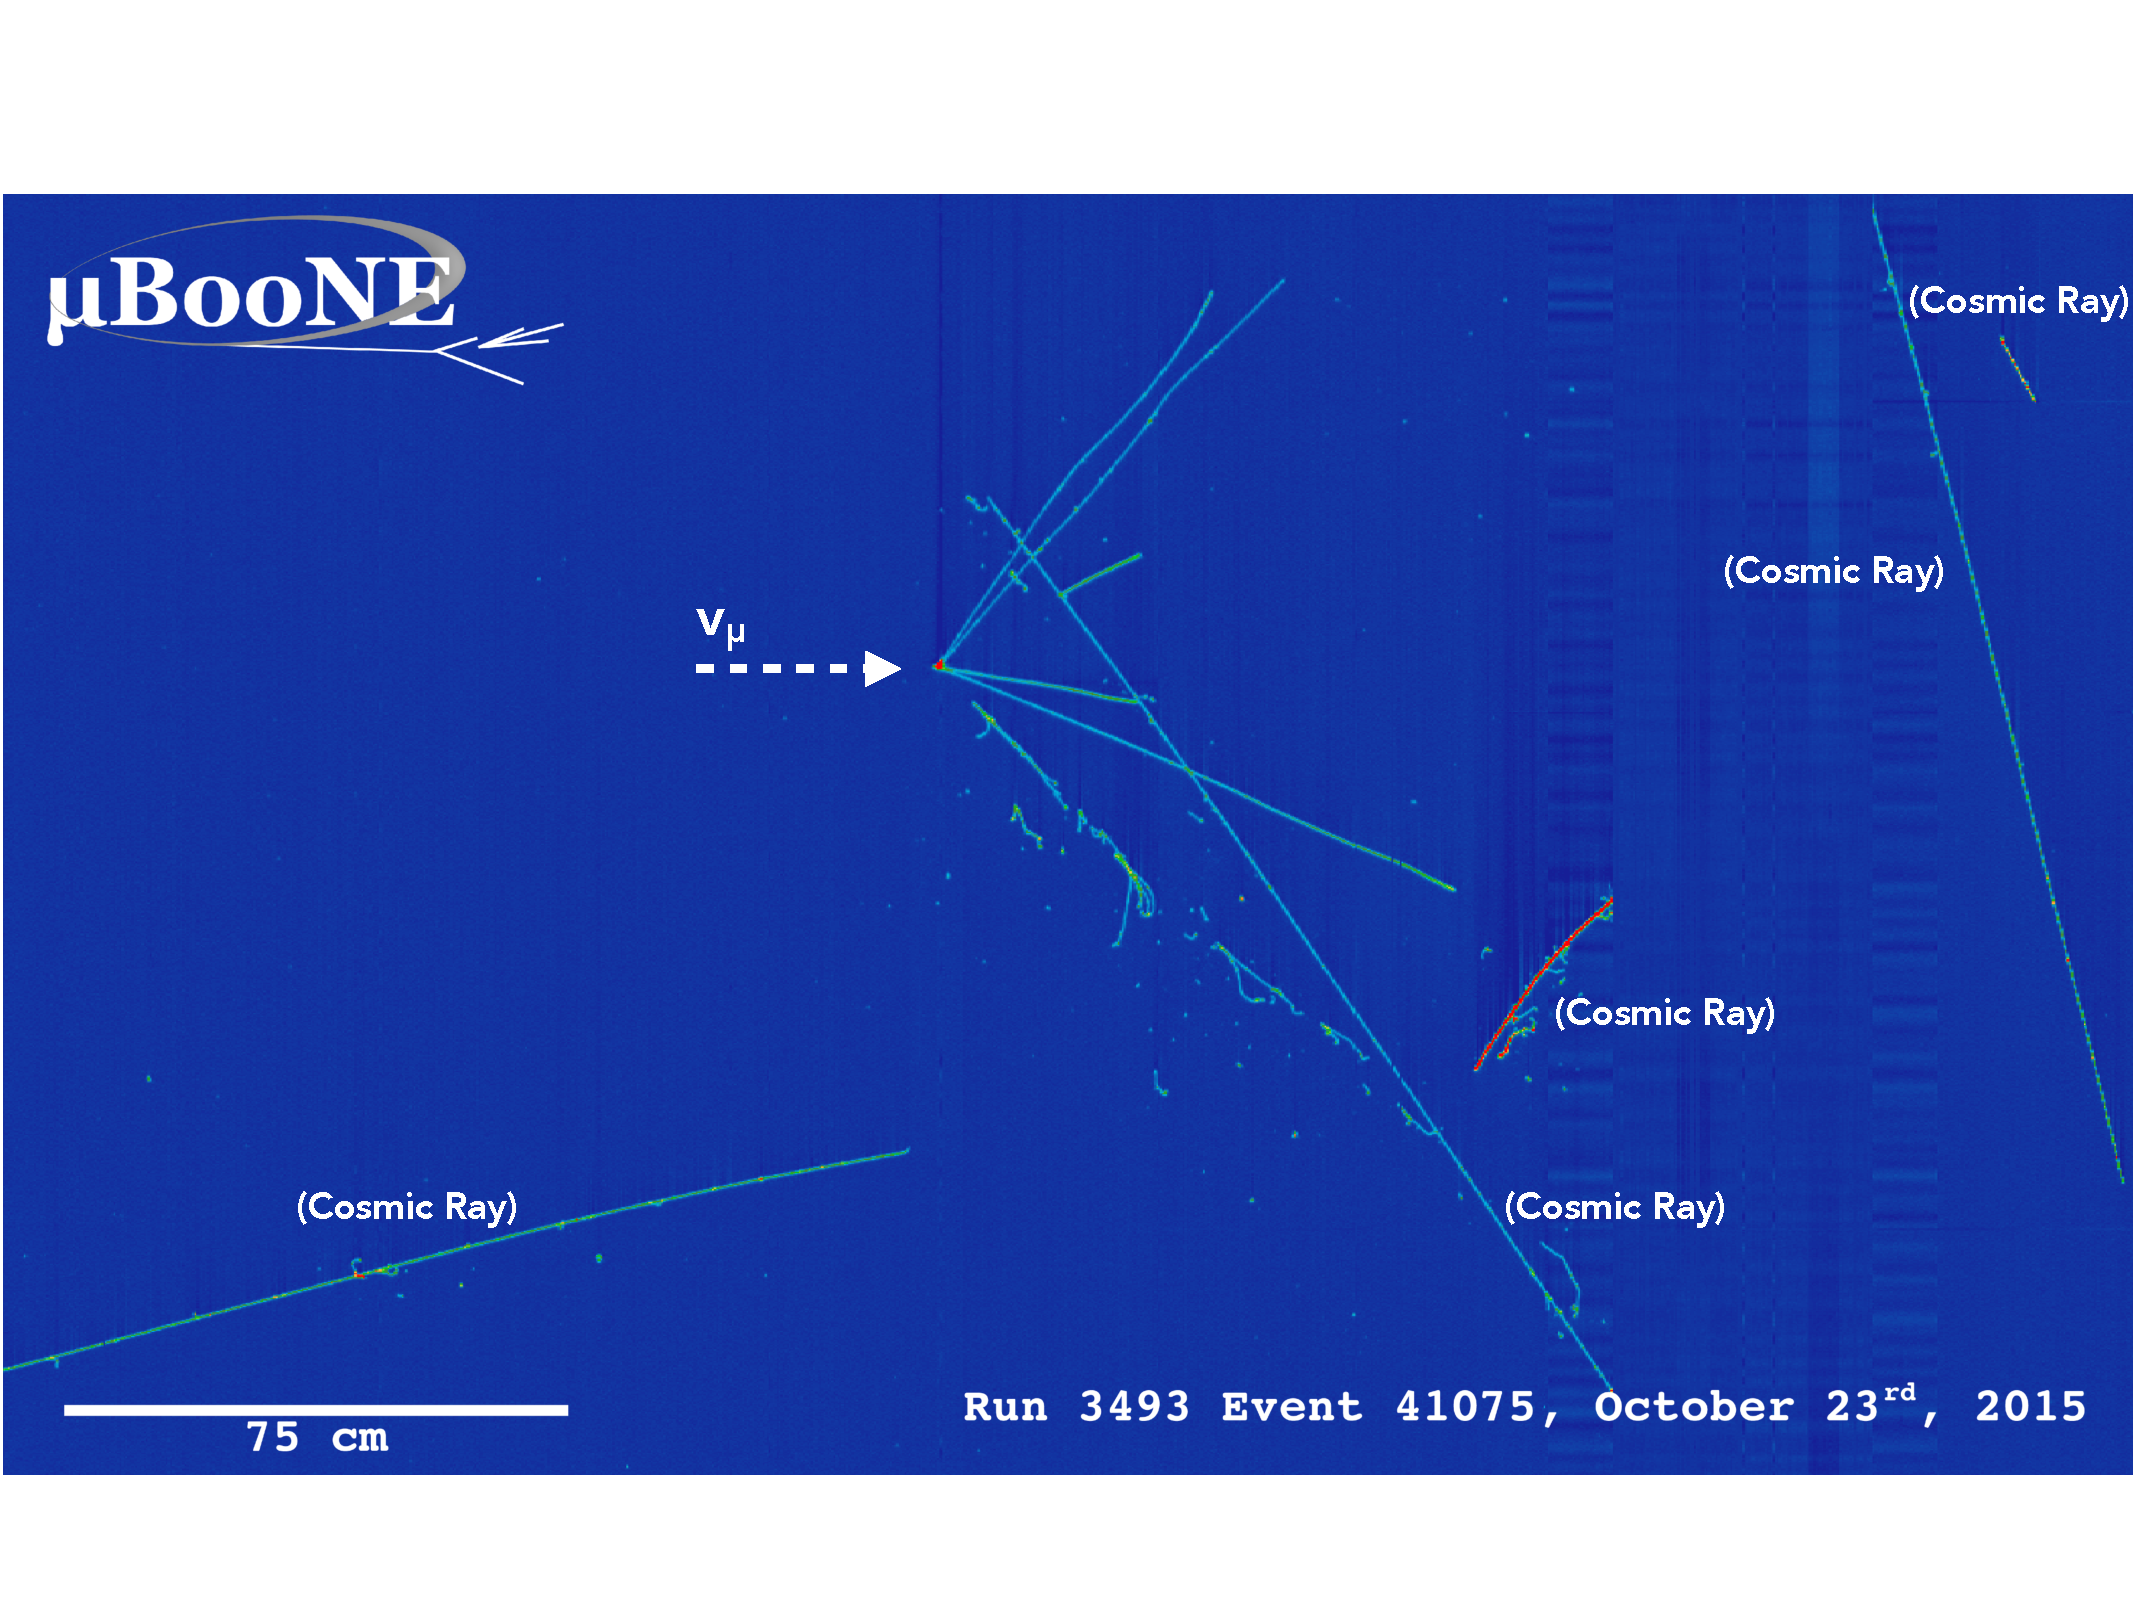
\includegraphics[width=.59\textwidth]{images/NeutrinoInteractions/evd_dis}
   \label{fig:evd_dis}} \\
\caption[Neutrino Interaction Modes from MicroBooNE Event Displays]{Events recorded by the MicroBooNE detector showing \acrshort{qe}~\subref{fig:evd_qe}, resonance~\subref{fig:evd_res}, and \acrshort{dis}~\subref{fig:evd_dis} events. The images show a 2D projection of the events, and display the final state particles coming from the neutrino interactions. Neutrinos come from the left. More details on the MicroBooNE event display are given in Section~\ref{sec:signal_formation}.}
\label{fig:evd_interactions}
\end{figure}





\subsection{Quasi-Elastic Interactions}
\label{sec:qe}

%+++++++++FIGURE+++++++++
% mpost fyW
% mpost fyZ
\begin{figure}[h]
\centering
\subfloat[][]
   {
   \centering
\begin{fmffile}{fyW}
  \begin{fmfgraph*}(50,50)
\fmfleft{i1,t1,t2,t3,t4,t5,t6,t7,t8,i2}
\fmfright{o1,p1,p2,p3,p4,p5,p6,p7,p8,o2} 
\fmf{fermion}{i1,vp}
\fmf{fermion}{vp,o1}
\fmf{photon,label=$W$,label.side=right}{vp,vl}
\fmf{fermion}{i2,vl}
\fmf{fermion}{vl,o2}
\fmflabel{$\nu_l$}{i2} 
\fmflabel{$l^-$}{o2}
\fmflabel{$n$}{i1} 
\fmflabel{$p$}{o1}
  \end{fmfgraph*}
\end{fmffile}
   \label{fig:diagramW}  
   } \qquad\qquad \qquad
   \subfloat[][]
   {
   \centering
 \begin{fmffile}{fyZ}
  \begin{fmfgraph*}(50,50)
\fmfleft{i1,t1,t2,t3,t4,t5,t6,t7,t8,i2}
\fmfright{o1,p1,p2,p3,p4,p5,p6,p7,p8,o2} 
\fmf{fermion}{i1,vp}
\fmf{fermion}{vp,o1}
\fmf{photon,label=$Z$,label.side=right}{vp,vl}
\fmf{fermion}{i2,vl}
\fmf{fermion}{vl,o2}
\fmflabel{$\nu_l$}{i2} 
\fmflabel{$\nu_l$}{o2}
\fmflabel{$n$}{i1} 
\fmflabel{$n$}{o1}
  \end{fmfgraph*}
\end{fmffile}
   \label{fig:diagramZ}
   } \\
\caption[Feynman Diagrams for Quasi-Elastic Scattering]{Example of Feynman diagrams of \acrshort{qe} interactions. A \acrshort{cc} with a $W$ exchange~\protect\subref{fig:diagramW}, and a \acrshort{nc} one, with a $Z$ exchange~\protect\subref{fig:diagramZ}.}
\label{fig:diagramWZ}
\end{figure}
%++++++++++++++++++++++++

At neutrino energies between $\sim0.1$ and $\sim1.5$ GeV, the primary way in which neutrinos interact with matter is via \acrshort{qe} interactions, as shown in Figure~\ref{fig:diagramWZ}. These interactions will now be discussed in details, as MicroBooNE deals with neutrinos mainly at these energies.
This section focuses on \acrshort{cc} interactions, which include the following processes: 
\begin{equation}
\nu_l + n \rightarrow l^- + p, \qquad \bar{\nu}_l + p \rightarrow l^+ + n,
\end{equation} 
for lepton flavour $l$, a neutron $n$ and proton $p$.


%Uncertainties in the neutrino interaction model are the largest uncertainties affecting the normalisation of events in the SBN detectors,
%
%Neutrino interactions on argon are simulated using the \g neutrino event generator. \g simulates each stage of the interaction including inclusive and exclusive differential cross sections off individual nucleons and the effects of the nuclear medium on final state particles as they propagate out of the target nucleus (final state interactions).

%Multi-nucleon correlation effects of the initial state are also a challenge in neutrino interactions and are not part of the present simulation.


Starting from Equation~\eqref{eqn:lagrangian}, an effective \acrshort{cc} Lagrangian can be written by requiring that the squared momentum transferred being smaller than the $W$ mass squared, $q^2 \ll M_W^2$, and so integrating out the $W$ boson, and by working at the first order in perturbation theory \cite{halzen}: 
\begin{equation}
\mathcal{L}_\text{eff} = - \frac{G_F}{\sqrt{2}} \left ( J^{\mu} {J_\mu}^\dagger \right ),
\end{equation}
where $G_F$ is the Fermi constant. The current $J^{\mu}$ is given by
\begin{equation}
J^{\mu} = \sum_l \bar{\nu}_l\gamma^\mu(1-\gamma^5)l + \sum_{ij} V_{ij}^\text{CKM} \bar{U}_i\gamma_\mu(1-\gamma_5)D_j,
\end{equation}
where $\nu_l$ and $l$ are the neutrino and lepton spinors with flavour $l$, $V^\text{CKM}$ is the Cabibbo–Kobayashi–Maskawa (CKM) matrix for the quark mixing, and $U$ and $D$ denote the up- and down-type quark spinors respectively.

%At the energy scales of QE interactions, the neutrino is not able to resolve the partons in the nucleon, but it rather interacts with the nucleon as a whole. Given the lack of knowledge of quantum-cromodynamics (QCD)  at low energy, it is not possible to analytically evaluate the neutrino cross section with protons and neutrons.
%Cross sections are then parametrised with ``form factor'' which effectively take into account the internal structure of the nucleons as well as their coupling with the lepton current.

The above Lagrangian describes the quark-level interaction as shown in Figure~\ref{fig:fyW_a}, but in reality, it is not possible to study neutrino interactions with free quarks, but rather with neutrons or protons. While the lepton current can be calculated exactly, this is not the case for the hadronic current. Problems arise in this case given the ignorance on the internal structure of the nucleons, and the inability to solve \acrfull{qcd} at low energies. 
Cross sections are then parametrised with ``form factors'' which effectively take into account the internal structure of the nucleons as well as their coupling with the lepton current, as schematically shown in Figure~\ref{fig:fyW_b}.
%For hadrons and nucleons, effective interactions are needed to parametrise this ignorance, as schematically shown in Figure~\ref{fig:fyW_b}.

% mpost fyW_a
% mpost fyW_b
\begin{figure}[]
\centering
\subfloat[][]
   {
   \centering
\begin{fmffile}{fyW_a}
  \begin{fmfgraph*}(40,25)
    \fmfleft{i1,i2}
    \fmfright{o1,o2}
    \fmftop{b}
    \fmf{fermion}{i1,v1,o1}
    \fmf{photon}{v1,b}
    \fmflabel{$q$}{i1}
%    \fmflabel{i2}{i2}
    \fmflabel{$q'$}{o1}
%    \fmflabel{o2}{o2}
    \fmflabel{$W$}{b}
  \end{fmfgraph*}
\end{fmffile}
   \label{fig:fyW_a}  
   } \qquad \qquad $\longrightarrow$ \qquad \qquad
   \subfloat[][]
   {
   \centering
\begin{fmffile}{fyW_b}
  \begin{fmfgraph*}(40,25)
    \fmfleft{i1,i2}
    \fmfright{o1,o2}
    \fmftop{b}
    \fmf{fermion}{i1,v1,o1}
    \fmf{photon}{v1,b}
    \fmfblob{.1w}{v1}
    \fmflabel{$N$}{i1}
%    \fmflabel{i2}{i2}
    \fmflabel{$N'$}{o1}
%    \fmflabel{o2}{o2}
    \fmflabel{$W$}{b}
  \end{fmfgraph*}
\end{fmffile}
   \label{fig:fyW_b}
   } \\
\caption[Feynman Diagrams and Form Factors]{$W$ interacting with a quark~\protect\subref{fig:fyW_a} and with a nucleon ~\protect\subref{fig:fyW_b}. It is not possible to solve \acrshort{qcd} at low energies and effective interactions, schematically shown as a blob in the picture, are considered when a $W$ interacts with a nucleon.}
\label{fig:fyW_ab}
\end{figure}


%Quasi-elastic scattering (e.g. $\nu_\mu + n \rightarrow \mu^- + p$) is modelled using an implementation of the Llewellyn-Smith model \cite{llewellyn}.
%
%If we associate the following momenta to the particles:
%\[
%\nu_\mu (k_1) + n (p_1) \rightarrow \mu^- (k_2) + p (p_2)
%\]
%we can then write the hadronic current as:
%\[
%\bra{p(p_2)} J_\mu \ket{n(p_1)} = \cos \theta_C\, \bar{u}(p_2) \Gamma_\mu u(p_1)
%\]
%where $\theta_C$ is the Cabibbo angle. 
The hadronic matrix element $\bra{p(p_2)} J_\mu \ket{n(p_1)}$ can then be expressed in terms of the most general Lorentz-invariant form factors:
\begin{equation}
\begin{split}
\bra{p(p_2)} J_\mu \ket{n(p_1)} = & \,\, \bar{u}^{(p)}(p_2)  [ \gamma_\mu F_V^1(q^2) + 
                              \frac{i\sigma_{\mu\nu}q^\nu}{2M}F_V^2(q^2) + 
                              \frac{q_\mu F_V^3(q^2)}{M} +                       \\
                              & \,\, \gamma_\mu\gamma_5 F_A(q^2) +
                              \frac{q_\mu \gamma_5}{M}F_P(q^2) +
%                              \frac{\gamma_5 (p_1 + p_2)_\mu }{M} F_A^3(q^2)  ] u^{(n)}(p_1),
                              \frac{i\sigma_{\mu\nu}q^\nu\gamma_5 }{2M} F_A^2(q^2)  ] u^{(n)}(p_1),
\end{split}
\end{equation}
where $q = k_1-k_2 = p_1-p_2$ is the momentum transfer, $M$ is the nucleon mass, 
%\[
%q = k_1-k_2 = p_1-p_2 \qquad M = 1/2(M_1 - M_2)
%\]
$F_V^{1,2,3}(q^2)$ are called vector form factors, $F_A(q^2)$ and $F_A^2(q^2)$ axial form factors and $F_P(q^2)$ pseudo-scalar form factor.

These form factors can be naively interpreted as the Fourier transform of the internal charge distribution of the nucleus \cite{halzen}. Assuming that this charge is distributed as $\rho(r) = \rho_0e^{-Mr}$, the form factors assume the form of a dipole: $F(q^2) \propto (1+q^2/m^2)^{-2}$, where $m$ is a parameter that needs to be measured experimentally.

%Current conservation at the hadronic vertex requires the two form factors $F_V^3(q^2)$ and $F_A^2(q^2)$ to be set to zero.
The two form factors $F_V^3(q^2)$ and $F_A^2(q^2)$ are set to zero as they violate G-parity.
$F_V^1(q^2)$ and $F_V^2(q^2)$ can be related via \acrfull{cvc} to electromagnetic form factors which are measured over a broad range of kinematics in electron elastic scattering experiments.  These observations have found that the dipole form works well for $Q^2 < 2.0\,\text{GeV}^2$, but deviations are seen at larger $Q^2$ (see, e.g. \cite{gayou}).
Extensions to $F_V^1(q^2)$ and $F_V^2(q^2)$, which parametrise these deviations, are typically used by the neutrino scattering community. One of the most recent parametrisations, called ``BBBA05'' form factors, are used in this work, which are defined in \cite{BBBA05}.


Two form factors remain: the pseudo-scalar $F_P(q^2)$ and the axial vector $F_A(q^2)$. The pseudo-scalar form factor is assumed to have the form suggested by the partially conserved axial current (PCAC) hypothesis
%\cite[\S 3.3.B]{llewellyn}
\cite{llewellyn}, which leaves the axial form factor $F_A(q^2)$ as the sole remaining unknown quantity. A dipole form is usually assumed for $F_A(q^2)$:
\begin{equation}
\label{eq:axial_mass}
F_A(q^2) = \frac{F_A(0)}{\left( 1+q^2/M_A^2 \right)^2}.
\end{equation}

$F_A(0)$ is well known from measurements of neutron beta decay ($F_A(0) = g_A$) and the $q^2$ dependence (parametrised by $M_A$, often referred to as ``axial mass'') of this form factor can only be determined in neutrino experiments and has been the focus of a large amount of experimental work over several decades.  
%$M_A$ remaining as the sole free parameter with a default value of $0.99$ GeV/c$^2$~\cite{GENIE_reweighting}. 
%
%$M_A^{\acrshort{cc}QE}$ contributes to the biggest systematic uncertainty in \acrshort{qe} scattering processes. The uncertainty on this parameter is taken into account in our cross-section calculation.

Usually, the Llewellyn Smith formulation is used for the neutrino-nucleon cross section, which is given by \cite{llewellyn}:
\begin{equation}
\label{eq:llsmith}
\frac{d\sigma}{dQ^2} = \frac{G_F^2M^2|V_{ud}|^2}{8\pi E_\nu^2} \left [ A(Q^2) \pm \frac{(s-u)}{M^2} B(Q^2) + \frac{(s-u)^2}{M^4} C(Q^2)  \right ],
\end{equation}
where the $(-)+$ refers to (anti)neutrino scattering, $M$ is the nucleon mass, $Q^2$ is the four-momentum transfer ($Q^2 = -q^2 > 0$), $E_\nu$ is the incident neutrino energy and $(s - u) = 4ME_\nu - Q^2 - m^2$, $m$ being the lepton mass. $A$, $B$ and $C$ are functions of $Q^2$ built from the vector ($F_V^{1,2}$), axial vector ($F_A$) and pseudoscalar ($F_P$) nucleon form factor \cite{llewellyn}.


As the \acrshort{nc} equivalent to \acrshort{cc} \acrshort{qe} interactions, neutrinos can undergo \acrshort{nc} elastic scatters, typically ejecting a nucleon from the nucleus. The available neutrino interaction modes are:
\begin{equation}
\begin{split}
\nu_\mu \, p & \rightarrow \nu_\mu \, p, \\
\nu_\mu \, n & \rightarrow \nu_\mu \, n. \\
\end{split}
\end{equation}
 As the hadronic current is similar, they are modelled very similarly to \acrshort{cc} \acrshort{qe} interactions.



\subsection{Resonance Production}
\label{sec:res}

Given enough energy and if the neutrino-nucleus centre of mass energy exceeds the mass of a delta baryon, neutrinos can send the struck nucleon to an excited state. In this case, the neutrino interaction produces a baryon resonance ($N^*$). The baryon resonance quickly decays, most often to a nucleon and single pion final state:
\begin{equation}
\nu_l + N \rightarrow l + N^* \rightarrow l + \pi + N',
\end{equation}
where $N, N' = n, p$. Other higher multiplicity decay modes are also possible as baryonic resonances created in neutrino-nucleon interactions can potentially decay to multi-pion final states. At the lowest energies, the process is dominated by production of the $\Delta(1232)$, as shown for example in Figure~\ref{fig:resDeltaPlus}.

%+++++++++FIGURE+++++++++
% mpost fyDeltaPlus
% mpost fyCoh
\begin{figure}[]
\centering
\subfloat[][]
   {
   \centering
\begin{fmffile}{fyDeltaPlus}
\begin{fmfgraph*}(50, 50)
\fmfstraight
\fmfleftn{i}{5}
\fmfrightn{o}{5}
\fmf{fermion}{i5,vt,o5}
\fmf{phantom}{i1,vb,o1}
\fmf{photon,label=$W$}{vt,vb}
\fmffreeze
\fmf{fermion}{i1,vb}
\fmf{double,label=$\Delta^{+}$}{vb,vr}
\fmf{fermion}{vr,o2}
\fmf{fermion}{vr,o1}
\fmflabel{$\nu_l$}{i5}
\fmflabel{n}{i1}
\fmflabel{n}{o1}
\fmflabel{$l^-$}{o5}
\fmflabel{$\pi^+$}{o2}
\end{fmfgraph*}
\end{fmffile}
   \label{fig:resDeltaPlus}  
   } \qquad\qquad \qquad
   \subfloat[][]
   {
   \centering
%\begin{fmffile}{fyDeltaPlusPlus}
%\begin{fmfgraph*}(40, 35)
%\fmfstraight
%\fmfleftn{i}{5}
%\fmfrightn{o}{5}
%\fmf{fermion}{i5,vt,o5}
%\fmf{phantom}{i1,vb,o1}
%\fmf{photon,label=$W$}{vt,vb}
%\fmffreeze
%\fmf{fermion}{i1,vb}
%\fmf{double,label=$\Delta^{++}$}{vb,vr}
%\fmf{fermion}{vr,o2}
%\fmf{fermion}{vr,o1}
%\fmflabel{$\nu_l$}{i5}
%\fmflabel{p}{i1}
%\fmflabel{p}{o1}
%\fmflabel{$l^-$}{o5}
%\fmflabel{$\pi^+$}{o2}
%\end{fmfgraph*}
%\end{fmffile}
\begin{fmffile}{fyCoh}
  \begin{fmfgraph*}(50,50)
\fmfleft{i1,t1,t2,t3,t4,t5,t6,t7,t8,t9,i2}
\fmfright{o1,p1,p2,p3,p4,p5,p6,p7,p8,p9,o2}
\fmf{fermion}{i2,vl}
\fmf{fermion}{vl,o2}
 \fmf{photon,label=$W$,label.side=right}{vl,vp}
 \fmfblob{.15w}{vp}
 \fmf{double,label.side=right}{vp,vt}
\fmf{fermion}{i1,vt}
\fmf{fermion}{vt,o1}
\fmffreeze
\fmf{double}{vp,p5}
\fmflabel{$\nu_l$}{i2} 
\fmflabel{$l^-$}{o2}
\fmflabel{$N$}{i1} 
\fmflabel{$N$}{o1}
\fmflabel{$\pi^+$}{p5}
  \end{fmfgraph*}
\end{fmffile}
   \label{fig:coherent}
   } \\
\caption[Feynman Diagrams for Resonance and Coherent $\pi$ Production]{Two examples of Feynman diagrams of pion production interactions: resonance~\protect\subref{fig:resDeltaPlus} and coherent~\protect\subref{fig:coherent}.}
\label{fig:pionProduction}
\end{figure}
%++++++++++++++++++++++++

In scattering off of free nucleons, there are seven possible resonant single pion reaction channels. Only listing the ones for neutrinos, resonance production can happen in both \acrshort{cc} (left) and \acrshort{nc}  (right) interactions:
\begin{align*}
\nu_\mu \, p & \rightarrow \mu^- \, p \, \pi^+,   &  \nu_\mu \, p & \rightarrow \nu_\mu \, p \, \pi^0, \\
\nu_\mu \, n & \rightarrow \mu^- \, p \, \pi^0,   &  \nu_\mu \, p & \rightarrow \nu_\mu \, n \, \pi^+, \\
\nu_\mu \, n & \rightarrow \mu^- \, n \, \pi^+,   &  \nu_\mu \, n & \rightarrow \nu_\mu \, n \, \pi^0, \\
 &                                               &  \nu_\mu \, n & \rightarrow \nu_\mu \, p \, \pi^-.
\end{align*}
To describe such resonance production processes, neutrino experiments most commonly use calculations from the Rein and Sehgal model \cite{rein_sehgal, fkr} and this is, in fact, the model used in the analysis presented in this thesis.

As for \acrshort{qe} interactions, the hadronic current is parameterised with form factors, both the vector and axial form factors are assumed to have a dipole form. Two parameters cannot be taken be taken from electron scattering, those are the equivalent as $F_A(0)$ and $M_A$ in Equation~\eqref{eq:axial_mass}, which have to be measured experimentally.

The analysis in this thesis also uses the Berger-Sehgal model \cite{berger_sehgal}, which improves upon the Rein-Seghal one in  using the available data on differential and total pion cross sections. In general, the pion scattering cross-section is significantly reduced compared to pion-nucleus Rein-Sehgal approximations in the $E_\pi < 1$ GeV region. 

\acrshort{nc} $\pi^0$ production is often the largest $\nu_\mu$-induced background in experiments searching for $\nu_\mu \rightarrow \nu_e$ oscillations, as the photons coming from the $\pi^0$ decay may mimic the signature of an electron neutrino interaction.
%In addition, as mentioned in Sec~\ref{}, \acrshort{cc} pion production processes can present a non-negligible complication in the determination of neutrino energy. For this reason, measuring and modelling nuclear effects in pion production processes has become paramount.  
%Once created in the initial neutrino interaction, the pion must escape the nucleus before it can be detected. Along its journey, the pion can rescatter, get absorbed, or charge-exchange thus altering its identity and kinematics. Improved calculations of such “final state interactions” (FSI) have been undertaken by a number of groups (





\subsection{Deep Inelastic Scattering}
\label{sec:dis}

In deep inelastic scattering (see Figure~\ref{fig:dis}), the neutrino scatters off a quark in the nucleon via the exchange of a virtual $W$ or $Z$ boson producing a lepton and a hadronic system in the final state. 
This breaks apart the nucleon, producing a jet of hadrons in an interaction mode known as \acrshort{dis}. This is the dominant neutrino interaction mode for neutrinos with energy above about 10 GeV.
Both \acrshort{cc} and \acrshort{nc} processes are possible:
\begin{equation}
\nu_\mu \, N  \rightarrow \mu^-   \, X, \qquad
\nu_\mu \, N  \rightarrow \nu_\mu \, X.
\end{equation}

There are only a few neutrinos undergoing \acrshort{dis} interactions at MicroBooNE energies, and for this reason, this interaction mode is not described in details here. Details on these interactions can be found in~\cite{halzen, zeller} and in this thesis they are modelled according to the \g neutrino simulator, which employs  a leading order model using the modifications suggested in~\cite{bodek_yang_dis} to describe scattering at low momentum transfer~\cite{GENIE_reweighting}.

%+++++++++FIGURE+++++++++
% mpost fyDIS
\begin{figure}[]
\centering
% See: https://wiki.physik.uzh.ch/cms/latex:feynman#deep_inelastic_scattering
\begin{fmffile}{fyDIS}
  \begin{fmfgraph*}(50,50)
    \fmfleft{ip,il}
    \fmfright{x1,x2,x3,o1,o2,o3,o4,ol}
    \fmfset{arrow_len}{10}
    % lepton
    \fmflabel{$\nu_l$}{il}
    \fmflabel{$l^-$}{ol}
    \fmf{fermion}{il,vl}
    \fmf{fermion}{vl,ol}
    \fmf{phantom,tension=0.6}{vl,vp}
    % proton
    \fmfv{l=$N$,l.a=-160}{ip} % l.a = label.angle
    \fmf{phantom,tension=1}{ip,vp,x1}
    \fmffreeze
    \fmfi{fermion}{vpath (__ip,__vp) scaled 1.01}
    \fmfi{fermion}
                  {vpath (__ip,__vp) scaled 1.01 shifted (-1.4, 6)}
    \fmfi{fermion}{vpath (__ip,__vp) scaled 1.01 shifted ( 1.4,-6)}
    \fmfblob{25}{vp}
    % X
    \fmfv{l=\mybrace{50} $X$,l.a=10}{x2}
    \fmf{fermion}{vp,x1}
    \fmf{phantom}{vp,x2} % to help \fmfi
    \fmf{phantom}{vp,x3} % to help \fmfi
    \fmfi{fermion}{vpath (__vp,__x2) scaled 0.98 shifted (0,2.2)}
    \fmfi{fermion}{vpath (__vp,__x3) scaled 0.92 shifted (0,4.5)}
    \fmffreeze
    % photon
    \fmf{photon,label=\vspace{-4pt}\hspace{5pt}{$W$},label.side=left}{vl,v}
    % parton
    \fmf{fermion}{vp,v}
    \fmf{fermion}{v,o2}
  \end{fmfgraph*}
\end{fmffile}
\caption[Feynman Diagrams for Deep Inelastic Scattering]{Feynman diagram for \acrshort{cc} neutrino \acrshort{dis} process.}
\label{fig:dis}
\end{figure}
%++++++++++++++++++++++++


%% See: https://wiki.physik.uzh.ch/cms/latex:feynman
%% mpost feyngraph1
%% mpost feyngraph2
%% mpost feyngraph3
%\begin{figure}[]
%\centering
%\subfloat[][] {
%\centering
%\begin{fmffile}{feyngraph1}
%  \begin{fmfgraph*}(50, 50)
%    \fmfstraight
%    \fmfleft{i2,g2,d,g1,i1}
%    \fmfright{o4,o3,o2,o1}
%    \fmftop{top}
%    \fmfbottom{bot}
%    % gluonS
%    \fmf{fermion,tension=1.4}{v,g1}
%    \fmf{fermion,tension=1.4}{g2,v}
%    \fmf{photon,tension=1.6,label=$Z$}{v,h}
%    \fmf{photon,tension=1.2,label=$Z$,l.s=right}{v1,h}
%    \fmf{dashes,tension=1.2,label=$H$,l.s=right}{h,v2}
%    % decay products
%    \fmf{phantom,tension=0.8}{top,v1}
%    \fmf{phantom,tension=0.8}{v2,bot}
%    \fmfshift{16 down}{o1}
%    \fmfshift{ 8 down}{o2}
%    \fmfshift{ 8 up}{o3}
%    \fmfshift{16 up}{o4}
%    \fmf{fermion,tension=1.8}{o2,v1,o1}
%    \fmf{fermion,tension=1.8}{o3,v2,o4}
%    % labels
%    \fmflabel{$\bar{q}$}{g1}
%    \fmflabel{$q$}{g2}
%    \fmflabel{$\nu_\ell$}{o1}
%    \fmflabel{$\bar{\nu}_\ell$}{o2}
%    \fmflabel{$\bar{b}$}{o3}
%    \fmflabel{$b$}{o4}
%  \end{fmfgraph*}
%\end{fmffile}
%\label{fig:resDeltaPlus}  
%} \qquad \qquad
%\subfloat[][]{
%\centering
%\begin{fmffile}{feyngraph2}
%  \begin{fmfgraph*}(50, 50)
%    \fmfstraight
%    \fmfleft{i2,g2,d,g1,i1}
%    \fmfright{o4,o3,o2,o1}
%    \fmftop{top}
%    \fmfbottom{bot}
%    % gluonS
%    \fmf{fermion,tension=1.4}{v,g1}
%    \fmf{fermion,tension=1.4}{g2,v}
%    \fmf{photon,tension=1.6,label=$W^\pm$}{v,h}
%    \fmf{photon,tension=1.2,label=$W^\pm$,l.s=right}{v1,h}
%    \fmf{dashes,tension=1.2,label=$H$,l.s=right}{h,v2}
%    % decay products
%    \fmf{phantom,tension=0.8}{top,v1}
%    \fmf{phantom,tension=0.8}{v2,bot}
%    \fmfshift{16 down}{o1}
%    \fmfshift{ 8 down}{o2}
%    \fmfshift{ 8 up}{o3}
%    \fmfshift{16 up}{o4}
%    \fmf{fermion,tension=1.8}{o2,v1,o1}
%    \fmf{fermion,tension=1.8}{o3,v2,o4}
%    % labels
%    \fmflabel{$\bar{q}$}{g1}
%    \fmflabel{$q$}{g2}
%    \fmflabel{$\nu_\ell/\ell^-$}{o1}
%    \fmflabel{$\ell^+/\bar{\nu}_\ell$}{o2}
%    \fmflabel{$\bar{b}$}{o3}
%    \fmflabel{$b$}{o4}
%  \end{fmfgraph*}
%\end{fmffile}
%   \label{fig:coherent}
%   } \qquad
%\subfloat[][]{
%\centering
%\begin{fmffile}{feyngraph3}
%  \begin{fmfgraph*}(50, 50)
%    \fmfstraight
%    \fmfleft{i2,g2,d,g1,i1}
%    \fmfright{o4,o3,o2,o1}
%    \fmftop{top}
%    \fmfbottom{bot}
%    % gluonS
%    \fmf{fermion,tension=1.4}{v,g1}
%    \fmf{fermion,tension=1.4}{g2,v}
%    \fmf{photon,tension=1.6,label=$Z$}{v,h}
%    \fmf{photon,tension=1.2,label=$Z$,l.s=right}{v1,h}
%    \fmf{dashes,tension=1.2,label=$H$,l.s=right}{h,v2}
%    % decay products
%    \fmf{phantom,tension=0.8}{top,v1}
%    \fmf{phantom,tension=0.8}{v2,bot}
%    \fmfshift{16 down}{o1}
%    \fmfshift{ 8 down}{o2}
%    \fmfshift{ 8 up}{o3}
%    \fmfshift{16 up}{o4}
%    \fmf{fermion,tension=1.8}{o2,v1,o1}
%    \fmf{fermion,tension=1.8}{o3,v2,o4}
%    % labels
%    \fmflabel{$\bar{q}$}{g1}
%    \fmflabel{$q$}{g2}
%    \fmflabel{$\ell^-$}{o1}
%    \fmflabel{$\ell^+$}{o2}
%    \fmflabel{$\bar{b}$}{o3}
%    \fmflabel{$b$}{o4}
%  \end{fmfgraph*}
%\end{fmffile}   \label{fig:resDeltaPlus}  
%} 
%\caption[Feynman Diagrams for Resonance and Coherent $\pi$ Production]{Two examples of Feynman diagrams of pion production interactions: resonance (left) and coherent (right).}
%\label{fig:pionProduction}
%\end{figure}


\subsection{Other Interaction Modes}
\label{sec:other_interactions}

In addition to resonance production, neutrinos can also coherently produce single pion final states. In this case, the neutrino coherently scatters from the entire nucleus $N$, transferring negligible energy to the target, as shown in Figure~\ref{fig:coherent}. The nucleus recoils but does not fragment, leaving it in the same final state as initial state.
Both \acrshort{cc} and \acrshort{nc} coherent pion production processes are possible:
\begin{equation}
\nu_\mu \, N  \rightarrow \mu^-   \, N \, \pi^+, \qquad
\nu_\mu \, N  \rightarrow \nu_\mu \, N \, \pi^0. 
\end{equation}
The Rein-Sehgal is again the model mostly used in event generators, with the Berger-Sehgal model being an improvement as discussed in the previous section.

Neutrino interactions can also produce final states involving strange quarks.
At neutrino energies below 2 GeV, Cabibbo suppressed single kaon production $\nu_\mu \, N \rightarrow \mu^- \, K^+ \, N$ is the dominant $K^+$ production mechanism~\cite{minerva_kp}. At higher energies, $K^+$ mesons arise via associated production accompanied by strangeness~$=-1$ baryons ($\Lambda$, $\Sigma^{\pm}$) or mesons ($K^-$, $\bar{K}^0$) such that there is no net change in strangeness ($\Delta S = 0$). This can occur through an intermediate resonance state or in \acrshort{dis} by hadronisation, the production of mesons and baryons from the struck quark. 
Measuring neutrino-induced kaon production is of interest primarily as a source of potential background for proton decay searches. Proton decay modes containing a final state kaon, $p \rightarrow K^+ \, \nu$, have large branching ratios in many SUSY GUT models~\cite{zeller}. Because there is a non-zero probability that an atmospheric neutrino interaction can mimic such a proton decay signature, estimating these background rates has become an increasingly important component to such searches.






\section{Nuclear Effects}
\label{sec:nuclear_effects}

The sections above described neutrinos interacting with free nucleons but in reality nucleons are aggregated in nuclei and nuclear effects alter the interactions and the products. In general, there are initial state effects that need to be taken into account as the nucleons are bound in the nucleus, as well as final state effects as the particles produced in the interactions need to pass through the nuclear matter to exit from the nucleus. 
While in the past neutrino experiments mainly used deuterium as target material, modern-day experiment use more complex nuclei to increase the overall interaction rates and because modern detector technologies require heavier elements (for example in the case of \acrshort{lartpc} detectors). When dealing with more complex nuclei, nuclear effects are no longer negligible and need to be taken into account. As a result, Equation~\eqref{eq:llsmith} is no longer valid, as it describes the interaction with a free nucleon. If the nucleon is bounded in a nucleus, it is important to take into account nuclear effects that produce sizeable modifications to Equation~\eqref{eq:llsmith}.
Finally, there will also be brand new interactions processes which are not present for free nucleons, as it will be described in the next sections.



\subsection{Basic Approximations and Fermi Motion}
\label{sec:fermi_motion}

In the majority of the cases, the \acrfull{ia} is the most commonly adopted to describe the interaction with a nucleus~\cite{ia_approximation}. The \acrshort{ia} approximation is based on the assumptions that at large enough momentum transfer the target nucleus is seen by the $W$ or $Z$ probe as a collection of individual nucleons and that the particles produced at the interaction vertex and the recoiling nucleon system evolve independently (see Figure~\ref{fig:impulse_approximation} for a pictorial representation of the \acrshort{ia} picture).
% As a consequence, IA neglects both statistical correlations due to Pauli blocking and the rescattering processes driven by strong interactions (FSI). 
As a result of this, the final cross section can be written as a cross section describing the neutrino-nucleon interactions, integrated all over possible states of the nucleon, weighted by a \acrfull{sf}:
\begin{equation}
\frac{d^2\sigma_\text{IA}}{dQ^2} = \int d^3p \, dE \, P (\mathbf{p}, E)\ \frac{d^2\sigma_\text{elem}}{dQ^2},
\end{equation}
where ${d^2\sigma_\text{elem}}/{dQ^2}$ corresponds to the one in Equation~\eqref{eq:llsmith}.
The function $P (\mathbf{p}, E)$ is the target \acrshort{sf}, i.e. the probability distribution of finding a nucleon with momentum $\mathbf{p}$ and removal energy $E$ in the target nucleus. It then encodes all the information about the initial (struck) particle.

%... where the sum in the picture is here represented by the integral over all possible states, and the P is normasile in such a way that intP = N nulceons

\begin{figure}[]
\centering
\subfloat[][]
   {\includegraphics[height=.28\textwidth]{images/NeutrinoInteractions/impulse_approximation_a}
   \label{fig:impulse_approximation_a}} \quad\quad\quad
\subfloat[][]
   {\includegraphics[height=.28\textwidth]{images/NeutrinoInteractions/impulse_approximation_b}
   \label{fig:impulse_approximation_b}} \\
\caption[Feynman Diagrams for the Impulse Approximation]{\protect\subref{fig:impulse_approximation_a}~Feynman diagram for the process $\nu_l + A \rightarrow l^- + A'$. \protect\subref{fig:impulse_approximation_b}~shows the \acrshort{ia} used to calculate the cross section for the process.}
\label{fig:impulse_approximation}
\end{figure}


In this approximation, the Fermi motion is embedded in the SF $P (\mathbf{p}, E)$, which needs to be characterised.
A simple and commonly used spectral function model is the global \acrfull{rfg} model~\cite{moniz}. Here, nucleons within the nucleus are modelled as non-interacting fermions inside a pervading nuclear potential, such that all momentum states are filled from the ground state upwards. The highest momentum state has momentum $p_F$, known as the Fermi momentum, which depends on the number of nucleons in a nucleus. 
This means that the \acrshort{sf} can be written as $P(\mathbf{p}, E) \propto \theta(p_F - |\mathbf{p}|)$, which then needs a Dirac $\delta$-function that ensures the conservation of energy. The energy of the struck nucleon (off-shell) can be written as:
\begin{equation}
E_\mathbf{p} = \sqrt{\mathbf{p}^2 + M^2} - \epsilon(\mathbf{p}),
\end{equation}
where $M$ is the nucleon mass and $\epsilon$ is the so-called interaction energy. The Smith–Moniz approach to the FG model \cite{moniz} is to approximate $\epsilon(\mathbf{p})$ by the constant average value $\bar{\epsilon}$, and conserve energy only on average. In this way, the spectral function takes the form
\begin{equation}
P(\mathbf{p}, E) = N \, \delta(\sqrt{\mathbf{p}^2 + M^2} - \bar{\epsilon} - M + E)\theta(p_F - |\mathbf{p}|),
\end{equation}
where $N$ is a normalisation constant. Overall, the Heaviside function gives rise to a sharp end in the \acrshort{sf} distribution, as can be seen from the green curve in Figure~\ref{fig:nucleon_momentum}, which shows the nucleon momentum distribution, defined as
\begin{equation}
\label{eq:np}
n(\mathbf{p}) = \int dE \, P(\mathbf{p}, E).
\end{equation}

\begin{figure}[]
\centering
\includegraphics[width=.70\textwidth]{images/NeutrinoInteractions/nucleon_momentum}
\caption[Fermi Motion Distributions]{Nucleon momentum distributions in an argon nucleus for several spectral functions as implemented in the \g neutrino event generator. The Bodek-Ritchie Fermi gas, relativistic Fermi gas and effective spectral function are shown. The distribution shown is $4\pi |\bm{p}|^2n(|\bm{p}|)$ as a function of $|\bm{p}|$, with $n(\bm{p})$ given by Equation~\eqref{eq:np} and with normalisation condition given by $ 4\pi \int d|\bm{p}||\bm{p}|^2n(|\bm{p}|) = 1$.}
\label{fig:nucleon_momentum}
\end{figure}

The \acrshort{rfg} spectral function treats all nucleons as feeling the same constant binding potential, whilst in reality this depends upon the local density of the nucleus. More sophisticated \acrfull{lfg} spectral functions use the local nuclear density $\rho(r)$ to build a nuclear potential that depends on the radial position of a nucleon within the nucleus $r$, following the density profile of the nuclear matter~\cite{nieves_lfg}.

Although a \acrshort{lfg}  model is more realistic than an \acrshort{rfg}  model, nucleons are still treated as non-interacting fermions (other than via the local nuclear potential). However, it is well known from electron scattering data that nucleon-nucleon interactions inside the nuclear medium can significantly alter the distribution of the initial state nucleon momenta \cite{huberts, rohe}. Nucleon-nucleon correlations introduce a high-momentum tail in the \acrshort{sf}s. There are variations of the \acrshort{rfg} and \acrshort{lfg} that allow to include these correlations, one example is the Bodek-Ritchie modification to the \acrshort{rfg} model~\cite{bodek_ritchie_fermigas}. This is shown in Figure~\ref{fig:nucleon_momentum}, and is the main model used in this thesis.

Beyond the energy conserving Dirac-$\delta$ shown above, these models are not explicitly functions of the removal energy $E$. More sophisticated \acrshort{sf} can be extracted by taking into account two and three-nucleon interaction potentials which give rise to nucleon-nucleon correlations. These \acrshort{sf}, for examples the ones derived in~\cite{ia_approximation}, depend explicitly on $E$, and have a high momentum tail.

Effective SF have also been calculated \cite{esf} that are able to reproduce the predictions obtained by the superscaling variable \cite{superscaling}. This SF also has a high momentum tail, as shown in Figure~\ref{fig:nucleon_momentum}.

In general, Fermi gas models need an additional modification to take into account the effect of Pauli blocking. Since nucleons are fermions, they follow Fermi-Dirac statistics which allows only two nucleons per energy level. Scattering which would take the nucleon to a new state already occupied by other nucleons are not allowed. For \acrshort{qe} interactions, which change a neutron to a proton, enough energy has to be transferred to the proton to avoid this problem or the reaction does not take place. In the \g simulator~\cite{GENIE}, used in MicroBooNE and in the work presented in this thesis, a suppression factor is included based on the simple requirement that the momentum of the outgoing nucleon exceeds the Fermi momentum $k_F$ for the nucleus in question.

A summary of the nuclear models used in this thesis is shown in Section~\ref{sec:simulation}.



\subsection{Final State Interactions}

As described in the previous section, many generators employed by neutrino experiments adopt the \acrshort{ia} in which neutrinos scatter on individual quasi-free nucleons. In this picture any neutrino-nucleus interaction can be factorised in a two-step process: in the first step, the neutrino scatters on a bound nucleon, and in the second step \acrfull{fsi} affect the hadrons produced in the first step. \acrshort{fsi} happen as pions and protons rescatter before exiting the nucleus. As an example, Figure~\ref{fig:fsi} shows how pions can be absorbed, can be scattered elastically, can produce new pions, or can exchange electric charge with nucleons.

\begin{figure}[]
\centering
\includegraphics[width=.50\textwidth]{images/NeutrinoInteractions/fsi}
\caption[Cartoon of Final State Effects]{Hadrons produced at the neutrino interaction vertex must still traverse the dense nuclear matter and they are then subject to \acrshort{fsi} before appearing in the detector. The image shows how pions can be absorbed, scattered, produce new pions or exchange electric charge with other nucleons. A similar picture can be drawn for nucleons. Image credit: \cite{golan_thesis}.}
\label{fig:fsi}
\end{figure}

Simulations used in major neutrino oscillation experiments, in their description of \acrshort{fsi} effects, rely on the model of \acrfull{inc} \cite{inc}. These cascade models assume the nucleus is an ensemble of quasi-free nucleons and the incident particle interacts in a series of encounters with single nucleons called a cascade (see Figure~\ref{fig:fsi}).
All interactions are governed by the cross section for the free processes, and the probability of interaction is governed by a mean free path $\lambda = 1/(\sigma\cdot\rho(r))$. The probability for a multitude of different interactions (e.g. elastic scatter, charge exchange, absorption) is calculated at each step based on the local nuclear density and, if necessary, such an interaction is simulated. This continues until the hadron leaves the nucleus. These cascade models have some limitations, they use a simple Fermi gas model to describe the distribution of the nucleons, effects of nucleon correlations must be included empirically and both the struck nucleon and the scattered hadron are likely to be off-shell, while they are treated as free particles.

\acrshort{fsi}s contribute significantly to the systematic uncertainties in neutrino oscillation measurements as they are extremely difficult to model or constrain with experimental data. In the simulation used in this thesis (\g), the intranuclear transport is handled by a subpackage called INTRANUKE and the model used for the \acrshort{inc} is called \texttt{hA}~\cite{GENIE_reweighting}. Rather than calculate a cascade of hadronic interactions as is done in a complete \acrshort{inc} model, the \texttt{hA} model uses the total cross section for each possible nuclear process for pions and nucleons. This is an empirical and data-driven model \cite{GENIE_reweighting} which uses data from Fe targets and extrapolates to other targets.

To conclude this section, it is important to note the nucleus will also affect the lepton in the final state. For targets with atomic number $Z$ greater than one, the effect of the electric field of the nucleus on the scattered lepton must be considered. Corrections due to this electric field are called Coulomb corrections. The corrections result in an acceleration (for $l^+$) or deceleration (for $l^-$) of the scattered lepton $l$, thus resulting in a variation of its momentum.

In this work, the measured neutrino cross sections at MicroBooNE will be compared to two \g simulations: one which includes the \texttt{hA} cascade model and no Coulomb corrections, and another that includes an updated cascade model called  \texttt{hA2014}~\cite{genie_production_release} (which includes a wide range of data~\cite{ashery} for other nuclei than Fe for $\pi^{\pm}$ so that much less extrapolation is needed), and Coulomb corrections as calculated by Nieves et al.~\cite{nieves, nieves2}.



\subsection{Nucleon-Nucleon Correlations and the Random Phase Approximation}
\label{sec:rpa}

MiniBooNE neutrino cross-section measurements \cite{miniboone} were much larger than the theoretical predictions. This is shown in Figure~\ref{fig:numu_xsec}, where the MiniBooNE and the NOMAD measurements, both on carbon, appear to differ in normalisation by about 30\%. The low energy MiniBooNE results are higher than expected from the Fermi Gas model with more sophisticated impulse approximation calculations assuming an axial mass $M_A = 1.0$ GeV from deuterium-based measurements. Indeed, a large nucleon axial mass of $M_A = 1.35\pm0.17$ GeV was needed to describe these data. Such large values for $M_A$ were in clear conflict with other electron and neutrino experiments which result in a value very close to 1 GeV ($M_A = 1.014 \pm 0.014$ GeV \cite{ma_bodek}). This is shown in Figure~\ref{fig:miniboone_ma}, where data from MiniBooNE now show the measured differential cross section as a function of the muon kinetic energy, and the black line shows the prediction with an axial mass of 1.32 GeV. This is the so-called MiniBooNE $M_A$ puzzle. 

\begin{figure}[]
\centering
\includegraphics[width=.7\textwidth]{images/NeutrinoInteractions/numu_xsec}
\caption[Existing Measurements of the $\nu_\mu$ Quasi-Elastic-Like Scattering]{Existing measurements of the $\nu_\mu$ \acrshort{qe}-like scattering cross section, $\nu_\mu n\rightarrow\mu^-p$, as a function of neutrino energy on a variety of nuclear targets. The free nucleon scattering prediction assuming $M_A = 1.0$ GeV is shown for comparison. Figure from \cite{zeller}.}
\label{fig:numu_xsec}
\end{figure}

It is currently believed that nuclear effects beyond the impulse approximation approach are responsible for the discrepancies noted in the experimental data. A more theoretically sound solution to the puzzle was obtained thanks to the inclusion of some standard nuclear effects such as multinucleon mechanisms~\cite{nieves_ma}.
In these mechanisms, the $W$ boson can be absorbed by nucleons belonging to correlated pairs and to two-nucleon currents arising from \acrfull{mec} which lead to the excitation of multinucleon or $2p2h$ (2-particles 2-holes) excitations. In these models, a substantial part of the cross section measured corresponds to events in which at least two nucleons are emitted.
The consideration of the $2p2h$ nuclear excitations allows to describe the MiniBooNE cross section $d\sigma/dT_\mu/d\cos\theta_\mu$ with values of $M_A$ around 1 GeV, as can been seen from the green curve in Figure~\ref{fig:miniboone_ma}.

\begin{figure}[]
\centering
\includegraphics[width=.7\textwidth]{images/NeutrinoInteractions/miniboone_ma}
\caption[MiniBooNE Cross Section and Predictions]{The muon angle and energy distribution $d^2\sigma/d\cos\theta_\mu dT_\mu$ for $0.80 < \cos\theta_\mu < 0.90$ from the MiniBooNE experiment \cite{miniboone}. The curves show different model predictions: the black line show the \acrshort{mc} obtained by increasing $M_A$ to 1.35 GeV, while the green line shows the model prediction with multinucleon effects and \acrshort{rpa} included. The two predictions are similar. Figure from \cite{nieves_ma}.}
\label{fig:miniboone_ma}
\end{figure}

However, not only multinucleon mechanisms but also \acrfull{rpa} corrections~\cite{nieves} turn out to be essential to find that axial masses consistent with the world average lead to a good description of the MiniBooNE data. 
\acrshort{rpa} is a method to describe microscopic quantum mechanical interactions in complex many-body systems. In this case, the many-body system is described by the mutual interactions of nucleons inside the nucleus, which cannot be resolved exactly. The overall effect of \acrshort{rpa} correlations is to account for the change of the electroweak coupling strengths, from their free nucleon values, due to the presence of strongly interacting nucleons.
\acrshort{rpa} corrections are dominant at low $Q^2$: the $W$ or $Z$ probe has small resolution and sees nucleons embedded in the nuclear potential. While at higher $Q^2$ \acrshort{rpa} corrections are negligible as the probe has high resolution and sees nucleons as almost free particles.

The cross section measurements presented in this thesis are compared to a default \g simulation that does not include \acrshort{rpa} and that uses an empirical model for the simulation of \acrshort{mec} events that reproduces MiniBooNE and NOMAD data~\cite{mec_dytman}. Moreover, the measurements are also compared  to an alternative configuration of \g that uses the Nieves et al. model~\cite{nieves, nieves2}, which folds interactions of correlated pairs and a \acrshort{rpa} corrections to describe interactions of many bodies into the calculation.





%\begin{SCfigure}[]
%\centering
%\includegraphics[width=.58\textwidth]{images/NeutrinoInteractions/miniboone}
%\caption{MiniBooNE cross section as a function of neutrino energy. In (a), shape errors are shown as shaded boxes along with the total errors as bars. In (b), a larger energy range is shown along with results from the LSND [56] and NOMAD [10] experiments. Also shown are predictions from the NUANCE simulation for an RFG model with two different parameter variations and for scattering from free nucleons with the world-average MA value.  Figure from \cite{miniboone}.}
%\label{fig:miniboone}
%\end{SCfigure}



%\begin{SCfigure}[]
%\centering
%\includegraphics[width=.50\textwidth]{images/NeutrinoInteractions/rpa}
%\caption{the \acrshort{rpa} correction factor as a function of $Q^2$}
%\label{fig:rpa}
%\end{SCfigure}





\section{Final Remarks}
\label{sec:remarks}

While most of our knowledge of neutrino cross sections around the $\sim 1$ GeV energy range comes from early experiments that collected relatively small data samples~\cite{zeller}, current experiments use heavy nuclei as target material, like hydrocarbon in the T2K and NO$\nu$A detectors, and argon in MicroBooNE. As described in the previous sections, nuclear effects seriously complicate the understanding of neutrino interactions and can greatly affect the sensitivity of neutrino oscillation experiments. 

Although many of the future experiments, such as DUNE~\cite{dune1, dune2, dune3} and the SBN program~\cite{sbn}, will all employ the \acrfull{lartpc} detection technology with argon as target material, experimental data for the neutrino-argon scattering process is scarce~\cite{ArgoNeuTCCincl, ArgoNeuTCCincl2}.

This thesis presents the first $\nu_{\mu}$ \acrshort{cc} inclusive measurement on argon at $\sim 0.8$~GeV of mean neutrino energy. The \acrshort{cc} inclusive channel is sensitive to some of the nuclear effects described in the previous sections and will be extremely valuable to future neutrino oscillation experiments. The signal topology for a $\nu_{\mu}$ \acrshort{cc} inclusive measurement is the presence and identification of a neutrino-induced muon track with or without accompanying particles. It is, therefore, the most inclusive cross section measurement that one can make, and due to the very clear signal definition allows straight-forward comparisons to theoretical models and other experiments. 

It is important to evaluate neutrino cross sections as a function of the kinematics of the outgoing muon as nuclear models will shape these distributions. Neutrino experiments have measured single differential cross sections as a function of the muon momentum ($d\sigma/dp_\mu$) or the cosine of the muon angle w.r.t.~the neutrino direction ($d\sigma/d\cos\theta_\mu$). Recently, experiments are also producing double-differential cross sections ($d^2\sigma/dp_\mu d\cos\theta_\mu$) as they provide a better insight in the properties of neutrino interaction with the nucleus and how the angle and the momentum of the lepton are correlated. For this reason, the analysis in this thesis will show both single and double-differential cross sections.

Some other modern experiments 
have also measured the $\nu_\mu$ \acrshort{cc} inclusive cross section. ArgoNeuT \cite{ArgoNeuTCCincl, ArgoNeuTCCincl2} and the T2K on-axis detector INGRID \cite{T2KCCinclINGRID,T2KCCinclINGRID2} published flux-integrated measurements. ArgoNeuT is the only experiment that published cross sections for neutrino-argon scattering to date, but at higher neutrino energy, around 5 GeV. SciBooNE \cite{SciBooNECCincl}, NOMAD \cite{NOMADCCincl}, MINOS \cite{MINOSCCincl}, and MINERvA \cite{MINERvACCincl,MINERvACCincl2} all published \acrshort{cc} inclusive cross sections as a function of a reconstructed neutrino energy. The only experiments with published double-differential data are event distributions from SciBooNE \cite{SciBooNECCincl} and cross section measurements from the T2K on-axis detector \cite{T2KCCinclND280}, both as a function of muon angle and muon momentum. T2K -- which has comparable beam energy to MicroBooNE -- was able to bin in four angular and five momentum bins. All flux-integrated or energy-dependent measurements are summarised in Figure~\ref{fig:pdg_cross_sections} from the PDG review article \cite{PDGReview}. This analysis provides a flux integrated measurement that can be added to a future Figure~\ref{fig:pdg_cross_sections}, as well as single differential and double differential cross sections as a function of muon momentum and angle, which allow to test generator predictions.

%\begin{SCfigure}[]
%\centering
%\includegraphics[width=.50\textwidth]{images/NeutrinoInteractions/pdg_cross_sections}
%\caption{Measurements of per nucleon $\nu_\mu$ and $\bar{\nu}_\mu$ \acrshort{cc} inclusive scattering cross sections divided by neutrino energy as a function of neutrino energy. From \cite{PDGReview}.}
%\label{fig:pdg_cross_sections}
%\end{SCfigure}

\begin{figure}[t]
\centering
\includegraphics[width=1.0\textwidth]{images/NeutrinoInteractions/pdg_cross_sections}
\caption[Measurements of $\nu_\mu$ and $\bar{\nu}_\mu$ Charged Current Inclusive Scattering]{Measurements of per nucleon $\nu_\mu$ and $\bar{\nu}_\mu$ \acrshort{cc} inclusive scattering cross sections divided by neutrino energy as a function of neutrino energy. From \cite{PDGReview}.}
\label{fig:pdg_cross_sections}
\end{figure}



















\chapter{The MicroBooNE Experiment}
\label{ch:microboone}

This chapter describes the technical details of the MicroBooNE experiment. Section~\ref{sec:bnb} describes the primary beamline from which MicroBooNE receives neutrinos: the \acrfull{bnb}. Details of the MicroBooNE \acrshort{lartpc} detector are then shown in Section~\ref{sec:detector}.
A comprehension of how a \acrshort{lartpc} works is crucial for understanding the results of the data analysis described in later chapters. This specific detector technology gives rise to certain backgrounds  which are relevant to MicroBooNE measurements and not for other experiments that use different detection techniques. Additionally, the knowledge of the neutrino beamline and the detector operation is precursory to the implementation of the neutrino flux and detector modelling uncertainties that affect the analysis presented in the next chapters. Sections~\ref{sec:trigger},~\ref{sec:readout_data_format},~\ref{sec:simulation} and~\ref{sec:detector_operations} will describe details of the trigger, readout electronics, simulation and detector operations, respectively.


\section{The Booster Neutrino Beamline}
\label{sec:bnb}

\begin{figure}[]
\centering
\includegraphics[width=.80\textwidth]{images/MicroBooNE/accelerator-chain}
\caption[Fermilab Accelerator Complex]{The Fermilab accelerator complex. Image source: \cite{doe}.}
\label{fig:accelerator-chain}
\end{figure}

The neutrino beam received by the MicroBooNE experiment is produced at the Fermi National Accelerator Laboratory (Fermilab) thanks to the Fermilab accelerator complex.
This complex, shown in Figure~\ref{fig:accelerator-chain}, is composed of four accelerators that work in tandem \cite{doe}: the linear accelerator (Linac), the Booster, the Recycler, and the Main Injector. These accelerators produce two primary proton beams, a low energy ($8$ GeV) proton beam from the Booster and a high-energy ($120$ GeV) beam from the Main Injector. Hitting a target, these proton beams produce secondary beams of pions, kaons, muons and neutrinos that serve a variety of experiments.
 
This section describes in some detail the production process of neutrinos through the \acrshort{bnb} beamline. Three sections will describe the main stages involved: the production and extraction of an 8 GeV proton beam, in Section~\ref{sec:beam}; the beam target and focusing horn which lead to a secondary meson beam, in Section~\ref{sec:target}; and the composition of the neutrino beam reaching the MicroBooNE detector, in Section~\ref{sec:composition}.


%NuMI is a tertiary beam resulting from the decays of pion and kaon secondaries produced in the NuMI target. Protons of $120$ GeV are fast-extracted from the Main Injector (MI) accelerator and bent downward by $58$ mrad toward Soudan, MN. The beam line is designed to accept $4.9 \times 10^{13}$ protons per pulse (ppp). The repetition rate is $0.75$ Hz, giving about $6\times 10^{20}$ protons on target per year, \cite{tdr}.

\subsection{Primary Proton Beam}
\label{sec:beam}

The Booster proton beam starts as a beam of negatively charged hydrogen ions $H^-$. The  $H^-$ ions are subjected to a linear accelerator using alternating electromagnetic fields that accelerate them to 400 MeV kinetic energy \cite{miniboone_flux}.
Electrons are removed from the $H^-$ ions through a carbon foil. The bare protons enter the 474-meter-circumference Booster synchrotron, which operates at a frequency of 15 Hz. Here, the protons are accelerated up to 8.89 GeV momentum. The protons are bunched in ``beam spills'' containing roughly $4 \times 10^{12}$ protons spaced throughout a 1.6 $\mu$s time window per spill. The protons are then directed toward a thick beryllium target.

The absolute number of \acrfull{pot} is measured by two toroids upstream of the target which are part of a larger beam monitoring system. The uncertainty on the \acrshort{pot} is on the order of 2\% \cite{miniboone_flux}. Additional beam characteristics are monitored by beam position monitors, a multi-wire chamber, and a resistive wall monitor.  This system measures beam intensity, timing, width, position, and direction of the proton beam.


\subsection{Beam Target and Focusing Horn}
\label{sec:target}

The beryllium target hit by the protons is made up of seven identical cylindrical segments of beryllium, to produce a cylinder 71.1 cm long and 0.51 cm in radius. These are contained within a sleeve (1.37 cm inner radius, 0.9 cm thickness) also made of beryllium, which is connected to each segment via three beryllium fins. The volume of air within the sleeve is circulated to provide cooling for the target.

When the protons hit the target, secondary particles are produced, including pions and kaons, which represent the primary source of neutrinos and anti-neutrinos. 
To enhance the neutrino beam, these secondaries are focused by a toroidal electromagnet (horn) placed around the target. 
Inside the horn, a toroidal magnetic field provides a restoring force for particles of a certain charge, and defocuses particles of the opposite charge, thus enhancing a $\nu_\mu$ beam while reducing $\bar{\nu}_\mu$ background (or vice versa) originating from the decay of the secondary particles. The more focused the mesons are before the decay, the more focused will the neutrino beam be once it reaches the detector, enhancing the flux. 
The focusing horn is made of aluminium and is pulsed with a 174 kA current. A drawing of the horn structure is shown in Figure~\ref{fig:horn}. 
\begin{figure}[]
\centering
\includegraphics[width=.80\textwidth]{images/MicroBooNE/horn}
\caption[MiniBooNE Horn]{The pulsed horn system. The outer conductor (grey) is transparent to show the inner conductor components running along the centre (dark green and blue). The target assembly is inserted into the inner conductor from the left side. In neutrino-focusing mode, the (positive) current flows from left-to-right along the inner conductor, returning along the outer conductor. The plumbing associated with the water cooling system is also shown. Adapted from \cite{miniboone_flux}.}
\label{fig:horn}
\end{figure}
The horn is 185 cm long and is composed of an inner and outer conducting cylinders. A positive current travels down the inner conductor, and arches back towards the front via the outer conductor, producing a magnetic field perpendicular to the beam direction within its volume and falls off as $1/r$. The inner conductor is placed just outside the beryllium target. Right outside the inner conductor, the strength of the magnetic field reaches 1.5 Tesla. Since the horn heats up due to the pulsed current and radiation, during running the inner conductor is being cooled with nozzles that spray water on it.
The direction of the current can be switched to focus the positively charged secondaries (as shown in Figure~\ref{fig:horn}), or the negatively charged secondaries, ultimately producing a beam primarily of  neutrinos (``neutrino mode'') or antineutrinos (``antineutrino mode''), respectively. 
The \acrshort{bnb} beamline is schematically shown in Figure~\ref{fig:bnb}.
The horn has a small field-free region, called the neck of the horn. The particles can pass through that region without being affected. The neck also allows the remaining proton beam to go through, without hitting the horn.
%A concrete collimator is located downstream of the target/horn assembly to absorb particles that would not otherwise contribute to the neutrino flux.

Focused charged pions and kaons travel through a 50-meter decay region: a cylindrical volume of air, in which pions and kaons decay, producing the tertiary neutrino beam which eventually reaches the detector. 
Remaining charged particles which have not yet decayed are blocked by an absorber made of concrete. The absorber stops the hadron component of the beam, while neutrinos and some of the muons pass through it.
By this point, the beam is composed almost entirely of neutrinos which propagate through the dirt before reaching the detector. 

\begin{figure}[]
\centering
\includegraphics[width=1.0\textwidth]{images/MicroBooNE/bnb}
\caption[Booster Neutrino Beamline]{Schematic of the \acrlong{bnb}.}
\label{fig:bnb}
\end{figure}









\subsection{Beam Composition}
\label{sec:composition}

\begin{figure}[]
\centering
\includegraphics[width=.70\textwidth]{images/MicroBooNE/flux}
\caption[Neutrino Flux Prediction at MicroBooNE]{Neutrino flux prediction at MicroBooNE. Figure from~\cite{flux_note}.}
\label{fig:flux}
\end{figure}

The analysis described in this thesis makes use of a data set collected when the horn was pulsed with a positive current, resulting in positively charged mesons being focused towards the beam axis, while negatively charged were deflected away. 
Pions are the most abundant particles produced in the target, and this results in a $\pi^+$ beam with a small contribution of $K^+$ and $\mu^+$. In the decay region, these secondary particles are left free to decay. Pions predominantly decay in $\mu^+$ and $\nu_\mu$, hence giving rise to the $\nu_\mu$ beam. At the same time, contamination from other neutrino states in pion decay are caused by either $\bar{\nu}_\mu$ or by $\nu_e$ coming from the decay of muons ($\mu^+ \rightarrow e^+ + \bar{\nu}_\mu + \nu_e$). $\bar{\nu}_\mu$ also come from the contamination in the beam from $\mu^-$ which are very forward going or very energetic and therefore are not deflected by the horn.

Neutrinos produced by the decay of kaons ($K^\pm$, $K^0$, $K_L^0$) also contribute to the flux. Due to the smaller kaon production rate in the target this is a minor contribution to the total neutrino flux. Almost the entire flux of $\nu_\mu$ with  energy below 2.5 GeV is contributed by events which originate from pion decay, while kaons contribute almost exclusively to $\nu_\mu$ beyond this energy. Most importantly, because of the broader range of decay channels, kaons contribute significantly to the $\nu_e$ flux, even at lower energies. A small fraction of $\bar{\nu}_e$ also arises from kaon decay.

In the end, the neutrino beam produced at the \acrshort{bnb} is a 93.6\% $\nu_\mu$ beam, with a contamination of $\bar{\nu}_\mu$ (5.86\%), $\nu_e$ (0.52\%) and $\bar{\nu}_e$ (0.05\%). Figure~\ref{fig:flux} shows the neutrino flux split in the contributions from the four neutrino states as modelled by the MiniBooNE beam simulation~\cite{miniboone_flux} and calculated at the MicroBooNE detector.

\section{The MicroBooNE Detector}
\label{sec:detector}

The MicroBooNE detector is located along the \acrshort{bnb} beamline, 470 m from the target.
It is a 60 metric ton fiducial mass (170 metric ton total mass) \acrshort{lartpc} detector \cite{det}, contained within a cylindrical cryostat, where charged particles traversing a volume of highly-purified liquid argon leave trails of ionisation electrons along their paths, and also create prompt ultraviolet scintillation photons. Ionisation electrons drift in an electric field to a system of three anode wire planes. Waveforms originate from drift electrons inducing signals on the three wire planes, as shown in Figure~\ref{fig:tpc}. The MicroBooNE \acrfull{tpc} is described in Section~\ref{sec:tpc}.
The scintillation photons are observed by \acrshort{pmt}s located behind the wire planes, described in Section~\ref{sec:pmt}.




\subsection{Time Projection Chamber}
\label{sec:tpc}

\begin{figure}[]
\centering
\includegraphics[width=.90\textwidth]{images/MicroBooNE/tpc}
\caption[MicroBooNE Time Projection Chamber]{Operational principle of the MicroBooNE \acrshort{lartpc}. Ionisation electrons from particles traversing the detector medium are drifted by an electric field past multiple planes of sense wires. The signals on those wires create several two-dimensional images of the event and can be combined to obtain a three-dimensional view of the event. \acrshort{pmt}s are also used to collect scintillation light, but are not drawn in this diagram. Image source:~\cite{det}.}
\label{fig:tpc}
\end{figure}

\begin{figure}[t]
\centering
\subfloat[][]
   {\includegraphics[width=.48\textwidth]{images/MicroBooNE/det_pic_1}
   \label{fig:det_pic_1}} 
\subfloat[][]
   {\includegraphics[width=.48\textwidth]{images/MicroBooNE/det_pic_2}
   \label{fig:det_pic_2}}
\caption[MicroBooNE Detector Pictures]{The MicroBooNE \acrshort{tpc} when it was inserted in the cryostat~\protect\subref{fig:det_pic_1}. The cathode is visible on the front right and the field cage, made of tubes, can also be seen. The inside the \acrshort{tpc}~\protect\subref{fig:det_pic_2}. The three wire planes are visible along the anode on the right, and the field cage tubes at the back.}
\label{fig:det_pic}
\end{figure}

The \acrshort{tpc} used in the MicroBooNE experiment, shown in Figure~\ref{fig:det_pic}, is a rectangular parallelepiped with dimensions 2.3 m (height) $\times$ 2.6 m (width) $\times$ 10.4 m (length, along the beam direction). The coordinate system adopted is shown in Figure~\ref{fig:tpc_coordinates}. 
\begin{figure}[]
\centering
\includegraphics[width=.90\textwidth]{images/MicroBooNE/tpc_coordinates}
\caption[MicroBooNE TPC Coordinate System]{Drawing of the MicroBooNE's \acrshort{tpc}. The \acrshort{tpc} is placed with its longest side in the beam direction. The anode-plane on which wires where signals are formed is on the right-hand side, as seen from the beam. The cathode, where the drift high voltage is applied, is on the left.}
\label{fig:tpc_coordinates}
\end{figure}
The 8256 stainless steel sense wires forming the three anode planes have a plane-to-plane spacing of 3 mm, and the wires on each plane are separated with a 3 mm wire pitch. The wires are connected to application-specific integrated circuits (ASICs) which operate at a liquid argon temperature of 87 K. 
While crossing the first two wire planes, consisting of 2400 wires at angles $\pm$60 degrees relative to the vertical, the electrons induce a signal on them. Subsequently, the electrons are collected by the third plane, made of 3456 vertically-oriented wires.
The electric field is created by a series of 64 2.54-cm diameter stainless steel pipes shaped into a rectangular loop, forming the field cage. The negatively charged cathode is held at a high voltage (operating voltage is 70 kV), and this voltage is incrementally stepped down across the field cage tubes with a voltage divider chain, with an equivalent resistance of 250 M$\Omega$ between each tube. The distance from centre-to-centre of adjacent field cage loops is 4 cm. This creates a uniform electric field within the \acrshort{lartpc}.





\subsection{Charge Signal}
\label{sec:signal_formation}

\begin{figure}[t]
\centering
\includegraphics[width=.80\textwidth]{images/MicroBooNE/evd_from_wf}
\caption[MicroBooNE Event Display from Raw Waveform]{Figure (a) shows a waveform from a collection plane wire (after noise filtering~\cite{noise_paper}). Figures (b) and (c) shows how the MicroBooNE event display is constructed, by displaying waveforms from each wire one next to the other. The display shows a candidate interaction vertex from a $\nu_\mu$ \acrshort{cc} interaction, where the final state proton and muon are visible.}
\label{fig:evd_from_wf}
\end{figure}

\begin{figure}[]
\centering
\includegraphics[width=1.0\textwidth]{images/MicroBooNE/evd_2}
\caption[MicroBooNE Event Display with Neutrino Candidate]{Event display showing raw data from a small region of the \acrshort{tpc} volume from the collection plane. The display shows a candidate $\nu_\mu$ \acrshort{cc} interactions, where the final state proton and muon are visible. The $x$ axis shows the collection plane wires (increasing wire-number from left to right) and the $y$ axis shows the drift-coordinate (increasing drift-time moving upwards). The scale bar applies to both the horizontal and vertical coordinates. The colour map shows the amount of collected charge on each wire per time tick. In this display the muon candidate is spatially contained in the detector and it decays. The Michel electron coming from the decay is also visible.}
\label{fig:evd}
\end{figure}

Ionisation electrons produced in the \acrshort{tpc} are detected as induced currents caused by their passage through sense-wires placed on the anode-plane. The same ionisation electrons will produce a signal on wires on all three planes since bias voltages are applied to ensure full transparency of the first two induction planes. As they pass by the first two wire-planes, electrons induce a bipolar signal. The signature on wires on the final plane, on which electrons are collected, is unipolar. Starting with a waveform from a single wire (Figure~\ref{fig:evd_from_wf}, step (a)), it is possible to visualise particles trajectories by displaying such waveform next to the waveforms from all the other wires, as done in steps (b) and (c) of Figure~\ref{fig:evd_from_wf}. This figure only shows part of the detector, where a $\nu_\mu$ \acrshort{cc} candidate vertex was identified. Figure~\ref{fig:evd} shows the complete candidate event, with the final state muon coming o a stop and decaying. In this figure, moving from the left to right, all the waveforms from the collection plane wires are displayed. For a single wire, the $y$ axis shows the recorded waveform in drift-time coordinate. Particle trajectory points visible in the lower part of the image are closer to the anode plane, as it took less time for the electrons originated in those points to drift and be collected by the collection plane wires. The $y$ axis in this figure can then be seen as the drift direction in the detector, while the $x$ axis shows the direction along the neutrino beam, as collection plane wires are displaced perpendicularly to this direction. In summary, Figure~\ref{fig:evd} shows a bird-eye view of particles interacting in the MicroBooNE detector.


\subsection{Light Collection System}
\label{sec:pmt}

Liquid argon is a bright scintillator, and sampling the light produced from interactions in the argon can bring powerful capabilities and information to complement the charge information. Scintillation light is produced by the formation and eventual radiative decay of excited argon dimers (or excimers) and is emitted in an isotropic distribution~\cite{doke, kubota}. Liquid argon produces a large amount of light per unit energy deposited (about 24,000 photons per MeV at 500 V/cm drift field) and is transparent to its own scintillation. The scintillation light has one prompt and one slow component with decay times of about 6 ns and 1.6 $\mu$s, respectively. 
Both components consist of photons with a wavelength of 128 nm (VUV). An example of raw waveform recorded by a single \acrshort{pmt} in MicroBooNE from a candidate neutrino interaction is shown in Figure~\ref{fig:raw_wf}, where both the fast and slow components are visible.

\begin{figure}[]
\centering
\includegraphics[width=.70\textwidth]{images/MicroBooNE/raw_wf}
\caption[MicroBooNE Optical Waveform]{A waveform from a MicroBooNE optical detector from the \acrshort{pmt} shaper (see Section~\ref{sec:readout_data_format}). One time-tick corresponds to 15.6 ns.}
\label{fig:raw_wf}
\end{figure}

Scintillation light is an important ingredient to the ultimate 3D reconstruction of particle interactions within a \acrshort{lartpc}. While the wire signals alone suffice to reconstruct 3D interactions, the absolute timing of an interaction (referred to as $t_0$) is unknown so there is ambiguity in the drift direction. However, measuring the scintillation light allows to clarify this ambiguity to high precision. In fact, the time scale of the production and propagation of the light (nanoseconds) is orders of magnitude faster than the ionisation electrons drift (milliseconds). Furthermore, the scintillation light from interactions is relatively localised, and therefore combining the measured \acrshort{pmt} signals with the physical position of the signal allows to match individual flashes of light with different interactions, which may have different interaction times $t_0$. The description of this flash-to-track matching is provided in Section~\ref{sec:flashmatch}. This is important to help tagging and rejecting cosmogenic backgrounds which may occur outside of the expected beam neutrino arrival times.

\begin{figure}[]
\centering
\includegraphics[width=.80\textwidth]{images/MicroBooNE/pmt_map}
\caption[MicroBooNE Light Collection System]{The MicroBooNE light collection system consists of a primary system of 32 optical units and a secondary optical system of four light guide paddles \cite{ub_paddle}. These are mounted behind the anode wire planes such that the view is not obscured by structural cross bars of the \acrshort{lartpc}. Image credit: \cite{det}.}
\label{fig:pmt_map}
\end{figure}

The light collection system in MicroBooNE consists of 32 8-inch-diameter Hamamatsu R5912-02mod cryogenic \acrshort{pmt}s. These \acrshort{pmt}s are mounted in a plane behind the three sense-wire planes. The physical location of these \acrshort{pmt}s is shown in Figure~\ref{fig:pmt_map}. These 32 \acrshort{pmt}s provide 0.9\% photocathode coverage. As shown in Figure~\ref{fig:pmt_pics}, in front of each \acrshort{pmt} an acrylic plate is mounted, coated with \acrfull{tpb}, an organic fluor which serves as a wavelength-shifting material. \acrshort{tpb} absorbs the VUV scintillation light photons and re-emits it at visible wavelengths detectable by the \acrshort{pmt}s, peaked at 425 nm.

%\begin{figure}[]
%\centering
%\includegraphics[width=.40\textwidth]{images/MicroBooNE/pmt_ub}
%\caption[MicroBooNE Optical Unit]{The MicroBooNE optical unit mount internal to the shield, with components labeled. Image credit: \cite{det}.}
%\label{fig:pmt_ub}
%\end{figure}

\begin{figure}[]
\centering
\subfloat[][]
   {\includegraphics[height=.43\textwidth]{images/MicroBooNE/pmt_ub}
   \label{fig:pmt_ub}} 
\subfloat[][]
   {\includegraphics[height=.43\textwidth]{images/MicroBooNE/pmt_pic_cryo}
   \label{fig:pmt_pic_cryo}}
\caption[MicroBooNE Optical Unit]{The MicroBooNE optical unit mount internal to the shield, with components labeled~\protect\subref{fig:pmt_ub}. Photo credit: \cite{det}. \acrshort{pmt}s mounted on the frame inside the MicroBooNE cryostat ~\protect\subref{fig:pmt_pic_cryo}. Photo credit: Reidar Hahn, Fermilab Visual Media Services.}
\label{fig:pmt_pics}
\end{figure}




\section{Triggers and Data Streams}
\label{sec:trigger}

Every event in MicroBooNE starts with a hardware trigger. The Fermilab accelerator division sends signals to MicroBooNE every time there is a neutrino beam spill. This trigger, called the ``\acrshort{bnb}'' trigger, causes a window to open the \acrshort{pmt} readout that lasts for 23.4 $\mu$s, and a window in the \acrshort{tpc} readout that lasts 4.8 ms. The beam trigger efficiency is 99.8\%~\cite{CaratelliThesis}. The data sample originating from the trigger is here called ``beam-on'' data sample.

The majority of the spills do not produce a neutrino interaction in the detector.  Indeed, simulations show that approximately only 1 in 600 beam spills produces a neutrino interaction in the detector. In order to reduce the amount of recorded data, not every spill is saved. A software trigger looks at light activity on the \acrshort{pmt}s in time-coincidence with the 1.6 $\mu$s beam spill reaching the detector. 
This activity may be caused by a neutrino interaction, coincident \acrshort{cr} activity, or some other coincident sources.
The software trigger reduces the data rate by a factor of 20 \cite{CaratelliThesis}. The signal efficiency loss through the trigger condition is negligibly small. Additionally, the trigger cut is superseded by a higher optical light deposition cut, later in the analysis. 

An additional trigger used in this work is the so-called ``EXT'' trigger, that mimics a \acrshort{bnb} trigger in the absence of neutrino beam. This trigger allows to record \acrshort{cr} data in order to measure the cosmogenic background that will affect the analysis. The data sample collected with this trigger is here called ``beam-off'' data sample.

In order to reduce the data volume to apply \acrshort{tpc} reconstruction algorithms to, an optical pre-filter is also run. This filter checks for optical activity within the time window of the beam and requires a minimum threshold of 20 \acrfull{pe} in the beam time window (a study on the impact of a \acrshort{pe} threshold on the analysis is described in Section~\ref{sec:beam_spill}).

The MicroBooNE simulation (described in Section~\ref{sec:simulation}), only includes simulation of events that contain neutrino interactions and does not contain events with only \acrshort{cr}s. In order to be compared to the beam-on data sample, events from the beam-off data stream are added to the simulation, normalising by the number of hardware triggers.
The event distributions presented in this thesis will either show simulation compared to beam-on minus beam-off data, or simulation plus beam-off data compared to beam-on data.




\section[Readout and Data Format]{Readout Electronics and Data Format}
\label{sec:readout_data_format}

MicroBooNE's readout electronics are responsible for forming, digitising, and recording signals associated with the \acrshort{tpc} and \acrshort{pmt} systems. 

The MicroBooNE \acrshort{tpc} electronics system is separated in ``cold'' electronics, submerged in liquid argon, and ``warm'' electronics, located outside of the cryostat. The cold electronics is responsible for amplifying and shaping signals produced on the sense wires. Performing these operations in a cold environment and in close proximity to the wires allows MicroBooNE to obtain a high signal-to-noise ratio, essential to obtain accurate particle identification with low detection thresholds. The warm electronics is responsible for digitising signals, compressing and formatting the data before it is sent to the data acquisition system.

The analogue signals from the 8256 sense wires in the \acrshort{tpc} pass through \acrfull{cmos} analogue front end ASICs which operate on cold motherboards at liquid argon temperatures~\cite{det}. The signals are then shaped and amplified by cold intermediate amplifiers before passing through a warm feed-through. The signals are received by custom-designed \acrshort{lartpc} readout modules, which digitise and process them. The \acrshort{tpc} wire signals are digitised at 16 MHz and then down-sampled in the digitisation process to 2 MHz (500 ns time-ticks). The \acrshort{tpc} system reads out three 1.6 ms frames of wire signal data associated with one event. This time is chosen based on how long it takes for ionisation electrons from the cathode side of the \acrshort{tpc} to drift to the anode wires (this time is 1.6 ms with the design drift field of 500 V/cm, but 2.3 ms with the current MicroBooNE drift field of 173 V/cm). One frame before and two frames after the trigger are collected, ensuring enough amount of data to identify a neutrino interaction, as well as all \acrshort{cr} signals that arrive soon enough before or after the neutrino which need to be reconstructed in analyses.

Similarly to the \acrshort{tpc}, the \acrshort{pmt} signals undergo separate shaping with a 60 ns peaking time to allow for digitisation of several samples on the rising edge of a signal for more precise timing reconstruction abilities. The \acrshort{pmt} signals are digitised at 64 MHz (15.625 ns time-ticks) and are then split into high-gain and low-gain channels which carry 18\% and 1.8\% of the total signal amplitude, respectively, to extend the dynamic range of the \acrfull{adc}.
The \acrshort{pmt} system records data in two different formats: $(i)$ in an unbiased way for a duration of 1500 samples (23.4 $\mu$s) which is opened by the beam-gate signal received on the trigger board. Neutrinos are expected to arrive $\sim$ 4 $\mu$s after this window is opened; $(ii)$ in a discriminated way (called ``cosmic discriminator'') before and after the 23.4 $\mu$s window. This is needed in order to reduce the amount of recorded data. Discriminated waveforms are read out for an interval of 6.4 ms, which well covers the 4.8 ms \acrshort{tpc} readout window: $[-1.6, +3.2]$ ms. The cosmic discriminator only saves waveforms that go above a threshold of 130 \acrshort{adc} ($\sim6.5$ effective \acrshort{pe}), and it only saves 40 samples ($\sim$ 0.6 $\mu$s). A dead-time of 45 samples follows every time a cosmic-discriminated waveform is recorded.











\section{Simulation}
\label{sec:simulation}


Beamline and detector simulations are intended to represent truth level estimations of neutrino production and interaction processes. These estimations serve as a baseline for comparison with collected data, as well as to estimate the backgrounds in the selected data samples. They are referred to as \acrfull{mc} simulations. There are a number of systems to model, and details to account for, to ensure the simulation precisely captures the state of the detector.

The flux of neutrinos at the MicroBooNE detector is simulated using a framework built by the MiniBooNE collaboration \cite{miniboone_flux}.
Neutrino interactions in the MicroBooNE detector are simulated using the \textsc{Genie} event generator \cite{GENIE}, which generates the primary interaction inside the argon nucleus, the production of all final-state particles in the nucleus (hadronisation), and the transport and rescattering of the final-state particles through the nucleus (\acrshort{fsi}).

\begin{figure}[t]
\centering
\includegraphics[width=1.0\textwidth]{images/MicroBooNE/sbn_cosmics}
\caption[Aerial View of Fermilab with Cosmic Rays]{Aerial view of Fermilab with the Booster neutrino beamline and the MicroBooNE detector. \acrshort{cr}s are the dominant background for many MicroBooNE data analyses.}
\label{fig:sbn_cosmics}
\end{figure}

Before proceeding with the detector simulation, there is one final step. MicroBooNE is a surface detector and is then subject to a high \acrshort{cr} rate, and many \acrshort{cr} muons cross the detector as shown in Figure~\ref{fig:sbn_cosmics}. The detector is placed in a pit 6 m below the surface with no overburden, and the estimated rate is of 5.5 kHz, which corresponds to an average of 25 \acrshort{cr} muons per recorded event. 
%
\begin{figure}[]
\centering
\subfloat[][]
   {\includegraphics[width=.48\textwidth]{images/MicroBooNE/beam_on_beam_off_a}
   \label{fig:beam_on_beam_off_a}} 
\subfloat[][]
   {\includegraphics[width=.48\textwidth]{images/MicroBooNE/beam_on_beam_off_b}
   \label{fig:beam_on_beam_off_b}}
\caption[``Cosmic Rays Only'' and ``Neutrino + Cosmic Rays'' Event Examples]{Examples of a ``Cosmic Rays Only'' event~\protect\subref{fig:beam_on_beam_off_a}, where no neutrino interacted in the detector but one \acrshort{cr}s muon interacts during the beam spill window, triggering the detector readout, and of a ``Neutrino + Cosmic Rays'' event~\protect\subref{fig:beam_on_beam_off_b}, where a neutrino inetracts in the detector triggering the readout, but a \acrshort{cr} muon can still be selected instead of the neutrino origin muon track.}
\label{fig:beam_on_beam_off}
\end{figure}
%
\acrshort{cr}s are the dominant background in the analysis documented in this thesis, and this background is here divided into two categories, illustrated Figure~\ref{fig:beam_on_beam_off}: 
\begin{itemize}
\item recorded events where no neutrino interacted in the detector (Figure~\ref{fig:beam_on_beam_off_a}). These events can be estimated directly from data, by recording events when the neutrino beam is off. These events give rise to background events when one of the \acrshort{cr} muons interacts in the 1.6 $\mu$s beam time window producing a flash that triggers the system, and its topology fakes a neutrino interaction;
\item recorded events where one neutrino interacted in the detector (producing a flash that triggers the system) but a \acrshort{cr} muon is instead selected (Figure~\ref{fig:beam_on_beam_off_b}).
\end{itemize}
While the first background does not need to be simulated, as it can be estimated from data events when the neutrino beam is off, the second background needs to be simulated as a neutrino interaction is also present.
This is done using the COsmic Ray Simulations for KAscade (\textsc{Corsika}) generator \cite{corsika}. There are a variety of configurable parameters in \textsc{Corsika} including primary interaction particle type and low-energy hadronic models that are explored in detail in a MicroBooNE public note~\cite{corsika_note}. 
After both neutrino and \acrshort{cr} interactions have been simulated, the products of these interactions are ready to be tracked through the detector.

The simulation of the MicroBooNE detector is based on \textsc{Geant4}~\cite{geant} and includes particle propagation, drift of ionisation electrons to the wire planes, as well as propagation of scintillation light to the \acrshort{pmt}s.
Ionisation due to \acrshort{cr}s also leads to a distortion of the electric field within the detector. The effect is the build-up of slow-moving positive ions in a detector which gives rise to the so-called ``space charge'' effect~\cite{space_charge}. This effect leads to a displacement in the reconstructed position of signal ionisation electrons, as well as variations in the amount of charge quenching experienced by ionisation throughout the volume of the \acrshort{tpc}. The MicroBooNE detector simulation includes the space-charge effect.
All simulation is carried out within the LArSoft framework~\cite{larsoft}.

The work documented in this thesis uses two different configurations of \textsc{Genie}, summarised in Table~\ref{tab:genie_tunes}. The first one, which is the baseline configuration used in MicroBooNE, uses the default \textsc{Genie} configuration in which Fermi motion is described by the Bodek-Ritchie Fermi gas model~\cite{bodek_ritchie}, \acrshort{qe} and resonant pion production interactions are modelled according to the Llewellyn-Smith~\cite{llewellyn} and the Rein-Seghal~\cite{rein_sehgal} models respectively, and an additional term is added that enhances \acrshort{qe}-like interactions that occur off of correlated nucleon pairs via an empirically driven meson exchange current~\cite{mec_dytman}. The second, alternative configuration, includes the Valencia model for \acrshort{qe} interactions paired with a local Fermi gas model~\cite{nieves, nieves2} and Kuzmin-Lyubushkin-Naumov~\cite{kuzmin} and Berger-Sehgal model~\cite{berger_sehgal} for resonant pion production. The alternative configuration represents a theoretically driven set of models relevant at MicroBooNE energies.

\begin{table}[t]
\begin{adjustwidth}{-1cm}{-1cm}
\caption[\textsc{Genie} Model Configurations]{The two \g model sets used in the analysis presented in this thesis.}
\label{tab:genie_tunes}
\centering
\begin{tabular}{ccc}
\toprule
Model element & \tuneone & \tunethree  \\
\midrule
Nuclear Model              & Bodek-Ritchie Fermi Gas \cite{bodek_ritchie}  & Local Fermi Gas \cite{nieves, nieves2}  \\
Quasi-Elastic              & Llewellyn-Smith \cite{llewellyn}          & Nieves \cite{nieves, nieves2}  \\
Meson-Exchange Currents    & Empirical \cite{mec_dytman}               & Nieves \cite{nieves, nieves2} \\
Resonant                   & Rein-Seghal \cite{rein_sehgal}              & Berger-Seghal \cite{berger_sehgal} \\
Coherent                   & Rein-Seghal \cite{rein_sehgal}              & Berger-Seghal \cite{berger_sehgal} \\
\acrshort{fsi}                        & hA \cite{GENIE_reweighting}         & hA2014 \cite{GENIE_reweighting} \\
\bottomrule
\end{tabular}
\end{adjustwidth}
\end{table}

\section{Detector Operations}
\label{sec:detector_operations}

The MicroBooNE detector has been recording neutrino beam data since the fall of 2015. Figure~\ref{fig:run1} shows the amount of \acrfull{pot} collected since the start of operations. The \acrshort{cc} inclusive cross-section analysis presented in this thesis utilises $1.6 \times 10^{20}$ \acrshort{pot} of data (called ``Run 1''), collected from February to October 2016. More recent data, not used for the analysis in this thesis, benefits from the installation of a \acrshort{cr} tagger system~\cite{crt}. 

\begin{figure}[t]
\centering
\includegraphics[width=0.85\textwidth]{images/MicroBooNE/run1}
\caption[Protons on Target over MicroBooNE Data-Taking Period]{Protons on target over MicroBooNE's two year data-taking period. Highlighted in red is the period used for the cross section analysis presented in this thesis.}
\label{fig:run1}
\end{figure}



\chapter{Event Reconstruction}
\label{ch:reconstruction}



This chapter describes the \acrshort{tpc} and optical reconstruction that is applied to all data events in order to go from the raw data recorded by the detector (as shown in the previous Chapter) to high-level reconstructed objects, like particles tracks and optical flashes of light, needed for the downstream analysis.
Sections~\ref{sec:optical_reco} and ~\ref{sec:tpc_reco} describe the \acrshort{tpc} and optical reconstruction respectively.

Section~\ref{sec:cosmic_removal} shows techniques for mitigating \acrshort{cr}s, the main background for many physics analyses at MicroBooNE. Section~\ref{sec:neutrino_reconstruction} describes how the \acrshort{tpc} reconstruction of neutrino candidate events is done, and Section~\ref{sec:flashmatch} shows how these \acrshort{tpc} reconstructed objects are matched to optical information.
Finally, Section~\ref{sec:momentum_reco} shows how the muon momentum is measured for the analysis in this thesis.



\section{Optical Reconstruction}
\label{sec:optical_reco}

The optical reconstruction collects raw waveforms recorded by individual \acrshort{pmt}s (as shown in Figure~\ref{fig:raw_wf}) and combines them to reconstruct ``flashes'', which represent optical activity in time across several \acrshort{pmt}s, usually caused by a single neutrino or \acrshort{cr} interaction in the \acrshort{tpc}. 

\subsubsection*{Signal Processing}

The first step performed in the optical reconstruction consists in merging the high and low gain channels described in Section~\ref{sec:readout_data_format} into a ``saturation-corrected'' waveform which tries to correct saturating high-gain pulses by using information from the low-gain channel.

\subsubsection*{Baseline Estimation}

The baseline estimation of the waveform is performed in two different ways depending on whether the waveform is coming from the cosmic or the beam discriminator, introduced in Section~\ref{sec:readout_data_format}. 
If the waveform comes from the cosmic discriminator, a constant value is used for the baseline, which is simply set to the first \acrshort{adc} value in the first recorded sample.
If the waveform comes from the beam discriminator, a more complex algorithm is used. A loop is done over all the waveform \acrshort{adc} recorded values, and the \acrfull{std} of neighbouring values is calculated. If the \acrshort{std} is low, it shows that there is no optical activity in that region. In such regions, the baseline is set to the same waveform \acrshort{adc} values. A loop along the waveform entries is done and, where a region with high \acrshort{std} is found, the baseline is estimated by doing a linear interpolation between the two low-\acrshort{std} adjacent regions. This procedure takes care of estimating the right baseline if there are fluctuations.
An example of a waveform with the estimated baseline is shown in Figure~\ref{fig:pmt_wf}.

\begin{figure}[]
\centering
\subfloat[][]
   {\includegraphics[width=.45\textwidth]{images/Reconstruction/pmt_wf}
   \label{fig:pmt_wf_1}} \quad 
\subfloat[][]
   {\includegraphics[width=.45\textwidth]{images/Reconstruction/pmt_wf_2}
   \label{fig:pmt_wf_2}} \\ 
\caption[PTM Waveform and Baseline Estimation]{An example of \acrshort{pmt} raw waveform from data in blue and the estimated baseline in green~\protect\subref{fig:pmt_wf_1}, and an enlargement of the waveform to show single \acrshort{pe} peaks~\protect\subref{fig:pmt_wf_2}.}
\label{fig:pmt_wf}
\end{figure}

\subsubsection*{Pulse Finding and Flash Reconstruction}

Once the baseline is determined, an algorithm that looks at the waveform ADCs going above a configurable threshold is run, in order to find pulses. Then, the flash reconstruction takes the identified pulses associated to each \acrshort{pmt} as input. The time range is divided into configurable intervals and pulses falling in the same time interval are identified. Once coincident pulses are found, an integration window of 8 $\mu$s is applied in order to collect all the late light. To avoid that another flash is claimed by coincident late light pulses, an 8 $\mu$s dead time window is also applied. In the case of two candidate flashes with a time difference smaller than 8 $\mu$s, only the one that deposits more \acrshort{pe} is saved.

The most interesting flashes are those happening during the 1.6 $\mu$s beam spill window, as the majority of them are induced by neutrino interactions. It is not possible to have multiple reconstructed flashes in that time window. In fact, it is smaller than 8 $\mu$s dead time window described above. In the case of more than one neutrino interactions or neutrino interactions with one or more \acrshort{cr}s happening during the beam spill window, two scenarios are possible. For simplicity, let's assume there are two interactions happening during that time, then: $(i)$ if the first interaction deposits less \acrshort{pe}s than then second one, the pulses of the first will be ignored, and a flash will be claimed with the pulses of the second one (although late light pulses of the first may contaminate the second claimed pulse), $(ii)$ if the first interaction deposits more \acrshort{pe}s than the second one, then a flash will be claimed at the time of the first interaction, and the pulses of the second interaction will be added to the first claimed pulse.  

The flash reconstruction also performs a constant background subtraction of 2 \acrshort{pe} per \acrshort{pmt} to account for a measured 250 kHz noise, that is then integrated over the 8 $\mu$\text{s} flash time window. Figure~\ref{fig:flash} shows a sketch of the flash reconstruction. 

\begin{figure}[]
\centering
\includegraphics[width=1.00\textwidth]{images/Reconstruction/flash_2}
\caption[Flash Reconstruction]{Schematic of flash reconstruction. The blue circles represent the MicroBooNE \acrshort{pmt}s, and the red line an example of particle track in the detector. The yellow \acrshort{pmt}s, that see light in time coincidence coming from the track, are clustered together to form a flash. }
\label{fig:flash}
\end{figure}












\section{\acrshort{tpc} Reconstruction}
\label{sec:tpc_reco}

This section briefly describes the reconstruction steps that lead to \acrshort{tpc} reconstructed objects like tracks, showers and vertices. 

The input data to the \acrshort{tpc} reconstruction consists of waveforms in the drift time of charge induced or deposited on the sense wires. 
These waveforms first pass through a filtering algorithm in order to reduce the noise introduced by the electronics~\cite{noise_paper}. 
After noise filtering, an algorithms identifies candidate peaks in the waveforms by requiring that the waveform goes above a configurable threshold. The threshold is currently set at 5 times the \acrshort{rms} noise which is about 300 electrons/tick on average on the collection plane~\cite{signal_paper_i, signal_paper_ii}. Candidate peaks in the waveforms are then fitted with a Gaussian shape in order to obtain a ``hit'' representing the charge deposited on a wire by an incident track. Hits are objects with a peak time and width and serve as the basic input to the reconstruction algorithms. Hits reconstructed from the waveforms displayed in Figure~\ref{fig:evd} are shown in Figure~\ref{fig:hits}.

\begin{figure}[]
\centering
\subfloat[][]
   {\includegraphics[width=.5\textwidth]{images/Reconstruction/hits}
   \label{fig:hits}}  \quad
\subfloat[][]
   {\includegraphics[width=.25\textwidth]{images/Reconstruction/3d_tracks}
   \label{fig:3d_tracks}} \\ 
\caption[Reconstructed Hits and Tracks]{Reconstructed hits and clusters (in different colours for different reconstructed particles)~\protect\subref{fig:hits} from the raw waveforms displayed in Figure~\ref{fig:evd}. Collection plane only. Figure~\protect\subref{fig:3d_tracks} shows a full view of the MicroBooNE \acrshort{tpc} with 3D reconstructed track. The event shown is the same as displayed in~\protect\subref{fig:hits} but zoomed out to show the full detector. Most of the tracks are \acrshort{cr} muons. Some tracks exit the detector in the $x$ (drift) direction, as not yet corrected for the interaction time $t_0$.}
\label{fig:reco_hits}
\end{figure}

Hits are then grouped into clusters.
The purpose of the cluster algorithm is to group hits which correspond to the same particle signature, i.e.~a track or a shower. 
MicroBooNE utilises the Pandora multi-algorithm pattern recognition framework, which handles the clustering of hits, as well as the reconstruction of 3D objects like tracks and showers \cite{pandora}.
The output of the Pandora multi-algorithm pattern recognition is structured in Particle Flow reconstructed particles, called ``PFParticles'' reconstructed particles, each one corresponding to a distinct track or shower, and their hierarchy, which identifies parent-daughter relationships and describes the particle flow in the observed interactions. 
A neutrino is created as part of the hierarchy and forms the primary parent particle for a neutrino interaction. 
Figure~\ref{fig:3d_tracks} shows 3D reconstructed tracks in the full volume of the MicroBooNE detector.

\acrshort{lartpc}s also provide excellent calorimetric information. Calorimetry can be used to make a measurement of a particle energy deposition, which is useful to construct the particle identification (PID). Calorimetry is used in the analysis presented in this thesis to identify stopping \acrshort{cr} background muons (see Section~\ref{sec:ct_stopmu}), and to distinguish muon candidate tracks from proton candidate tracks (see Section~\ref{sec:selection_muon_candidate}). It is possible to reconstruct a particle deposited energy per unit of length $dE/dx$ from the waveforms induced by the ionisation electrons, such as the one in Figure~\ref{fig:evd_from_wf}(a). The area below the waveform is divided by the track segment that crosses that particular wire, in order to estimate the particle $dQ/dx$ in \acrshort{adc}/cm. This variable is then calibrated in simulation and data using \acrshort{cr} muons~\cite{calibration}, so to obtain a $dQ/dx$ in $e^-$/cm. Additional correction are also applied, that take into account electron lifetime and recombination~\cite{birks_argoneut}. 
In argon, the average energy expended per ion pair ($W$-value) is 23.6 eV, so that the number of electrons produced per MeV of deposited energy is approximately 42370 $e^-$/MeV. Using this relation, the particle deposited energy per unit of length $dE/dx$ can be estimated.

The analysis does not make use of the particle $dE/dx$ but uses a reconstructed truncated mean charge deposition along the length of the track $\braket{dQ/dx}_\text{trunc}$ in $e^-$/cm, shown in Figure~\ref{fig:dqdx} both for data and simulation.  
To calculate the truncated mean, the median $m$ and the standard deviation $\sigma$ of all the $dQ/dx$ values per hit in the track are calculated. Hits with $dQ/dx$ greater than $m - \sigma$ and smaller than $m + \sigma$ are then selected. Finally, the mean value of the $dQ/dx$ of the selected hits is defined as truncated mean $\braket{dQ/dx}_\text{trunc}$.
The truncated mean is used instead of the mean or median of the full distribution because it is less sensitive to fluctuations.
The truncated mean is obtained per plane, with only the collection plane being used in this analysis. The data and simulation entries at $\braket{dQ/dx}_\text{trunc} \sim 0$ are due to tracks aligned with the drift direction. In this case, all of the charges arrive on very few collection plane wires, and the hit reconstruction tends to assign this large charge deposition to many hits. This leads to some charge being missed ``between'' the fitted hits.

\begin{figure}[]
\centering
\subfloat[][]
   {\includegraphics[width=.5\textwidth]{images/Reconstruction/dqdx_trunc_calib}
   \label{fig:dqdx_trunc_calib}}  
\subfloat[][]
   {\includegraphics[width=.5\textwidth]{images/Reconstruction/dqdx_trunc_calib_protonzoom}
   \label{fig:dqdx_trunc_calib_protonzoom}} \\ 
\caption[Track $dQ/dx$ Distribution]{Distributions of the truncated mean $\braket{dQ/dx}_\text{trunc}$ for the muon candidate track~\protect\subref{fig:dqdx_trunc_calib}. Black points are data points. The coloured histograms shows the simulation (stacked). Plot~\protect\subref{fig:dqdx_trunc_calib_protonzoom} is an enlargement of plot~\protect\subref{fig:dqdx_trunc_calib}, showing that a proton track is selected as muon candidate for higher values of $\braket{dQ/dx}_\text{trunc}$.}
\label{fig:dqdx}
\end{figure}


















\section{Cosmic Ray Removal}
\label{sec:cosmic_removal}

As described in Section~\ref{sec:simulation}, MicroBooNE is a surface detector and is then subject to constant exposure of cosmogenic radiation from the atmosphere. \acrshort{cr} removal is therefore fundamental for any physics analysis.

Immediately after the reconstruction, the hits are passed to the Pandora framework that performs PFParticle reconstruction. Pandora is run in two different modes \cite{pandora}:
\begin{itemize}
\item \pc, optimised for the reconstruction of \acrshort{cr}s and their daughter delta rays;
\item \pn, optimised for the reconstruction of neutrino interactions. 
\end{itemize}
Pandora is first run in \pc mode over all reconstructed hits. The output reconstructed particles are analysed by a series of \acrshort{cr} tagging algorithms described in the following sections. PFParticles identified as \acrshort{cr}s are removed together with their daughter reconstructed particles, as well as their reconstructed hits. By default, \pc reconstructs \acrshort{cr}s as tracks and delta rays as showers. Removing all the hits of the daughter particles avoids leaving the delta ray debris laying around. If a PFParticle shares hits with another reconstructed particle which has not been tagged, the shared hits will not be removed. 
The remaining hits are passed again to the Pandora framework, which is now run with the \pn configuration. The chart in Figure~\ref{fig:cosmic_removal_chart} shows all these steps. The next sections describe how the \acrshort{cr} tagging is performed, while the rest of the analysis, performed with \pn reconstructed objects, is described in the following chapters. 

\begin{figure}[]
\centering
\includegraphics[width=1.0\textwidth]{images/Reconstruction/cosmic_removal_chart}
\caption[Cosmic Tagging Chart]{Chart showing the steps to remove \acrshort{cr}s before the data analysis takes place.}
\label{fig:cosmic_removal_chart}
\end{figure}



%**********************************************************
\subsection[Cosmic Tagging: Geometry]{Cosmic Tagging Using Geometry and Timing}

Tracks which are partially found to lie outside of the beam-spill drift window (before the trigger time and after the trigger time plus one drift length) are removed. These tracks must have entered the \acrshort{tpc} at a time which is inconsistent with the trigger time.

\acrshort{cr}s can also be identified  if their track both enters and exits the \acrshort{tpc}. 
A \acrfull{fv} contained in the active volume of the \acrshort{tpc} within 30 cm from the top and the bottom of the \acrshort{tpc}, 10 cm from the \acrshort{tpc} borders along the drift direction, and 20 cm from the \acrshort{tpc} ends, is defined.
A track trajectory is considered to enter or exit the \acrshort{tpc} if the track endpoints are outside the \acrshort{fv}. 
The \acrshort{fv} borders have been chosen after a dedicated optimisation giving the best \acrshort{cr} background reduction. The 30 cm from the top and the bottom are needed to remove most of the \acrshort{cr}s whose start and end points are mis-reconstructed and shifted due to space-charge effect. A smaller \acrshort{fv} is used in the event selection described in Section~\ref{sec:fiducial_volume}). 






\subsection[Cosmic Tagging: Optical]{Cosmic Tagging Using Optical Information}
\label{sec:ct_optical}

\acrshort{cr}s can also be identified if they are not compatible with the flash reconstructed in the neutrino beam spill window. An algorithm looks at the compatibility between flashes and tracks. The algorithm first selects the flash in the 1.6 $\mu$s beam spill window, then takes all the PFParticles reconstructed by the \pc algorithms and it simulates the associated light patterns expected on the \acrshort{pmt}s, introducing a ``flash hypothesis''. Details on the light simulation will be provided in  Section \ref{sec:flashmatch}.
The hypothesis flash centre $Z_\text{flash}$ along the beam direction is calculated averaging the \acrshort{pmt} positions of the \acrshort{pmt}s that contribute to the flash, weighting for the \acrshort{pe} simulated per \acrshort{pmt}:
\begin{equation}
\label{eq:flash_z}
Z_\text{flash} = \left<Z\right> = \left ( \sum_{i=0}^{32} Z_{\text{PMT}_i} \times \text{PE}_i \right ) / \sum_{i=0}^{32} \text{PE}_i.
\end{equation}
Its uncertainty $\Delta Z_\text{flash}$ takes into account the variance of the \acrshort{pmt} positions:
\begin{equation}
\Delta Z_\text{flash} = \sqrt{ \text{Var}(Z) } = \sqrt{ \left<Z^2\right> - \left<Z\right>^2 },
\end{equation}
where $Z_{\text{PMT}_i}$ is the $z$ coordinate of the $i^\text{th}$ \acrshort{pmt} and $\text{PE}_i$ are the photoelectrons detected by that \acrshort{pmt} for that particular flash.

%Assuming the PFParticle hierarchy has neutrino origin, the tracks in the hierarchy are shifted along $x$ by $t_0\times v_\text{drift}$.

If the PFParticle has neutrino origin and represents the whole neutrino interaction in the detector, the reconstructed and hypothesis flashes are expected to agree. If the PFParticle represents only part of the neutrino interaction, the hypothesis flash is expected to be smaller than the reconstructed flash. If the PFParticle has \acrshort{cr} origin, the hypothesis and reconstructed flashes should disagree.

The PFParticle is tagged as \acrshort{cr} if at least in one \acrshort{pmt} the number of the reconstructed \acrshort{pe}s ($PE_\text{reco}$) and the number of hypothesis \acrshort{pe}s ($PE_\text{hypo}$) satisfy
\begin{equation}
\frac{PE_\text{hypo} - PE_\text{reco}}{\sqrt{PE_\text{hypo}}} > 3,
\end{equation}
meaning that the hypothesis is 3$\sigma$ larger than the reconstructed one. In addition, to tag PFParticles as \acrshort{cr}s, the $z$ centre of the two flashes must satisfy
\begin{equation}
Z_\text{hypo} \notin \left [ Z_\text{reco}-\Delta Z_\text{reco}, Z_\text{reco}+\Delta Z_\text{reco}  \right ],
\end{equation}
where $Z_\text{reco}$ is the reconstructed beam flash. This last check has been added to ensure that neutrino related tracks are not tagged.










\subsection[Cosmic Tagging: ACPT]{Cosmic Tagging Using Anode/Cathode Piercing Tracks}

A different algorithm identifies \acrshort{cr}s that pierce the two sides of the detector: the anode and the cathode planes. 
Because of the slow electron drift velocity, reconstructed track information along the drift-coordinate has an offset with respect to the true energy deposition location, as shown in Figure~\ref{fig:acpt_1}. This offset can be corrected only if the time $t_0$ at which the track enters the detector volume is reconstructed. This section presents a method developed for reconstructing the $t_0$ of the track for the subset of \acrshort{cr} tracks which pierce either the \acrshort{tpc} anode- or cathode-plane: \acrfull{acpt}.

%\begin{figure}[]
%\centering
%\includegraphics[width=.65\textwidth]{images/Reconstruction/acpt}
%\caption[Example of Anode Crossing Cosmic Track]{Reconstructed tracks need to be corrected for their time offset introduced by the finite velocity of the drifting electrons. In this sketch, a true \acrshort{cr} track enters the detector from the top and exits from the anode plane, but the time offset makes the track look like it is stopping in the TPC.}
%\label{fig:acpt}
%\end{figure}

\begin{figure}[]
\centering
\subfloat[][]
   {\includegraphics[height=.41\textwidth]{images/Reconstruction/acpt_1}
   \label{fig:acpt_1}} \quad 
\subfloat[][]
   {\includegraphics[height=.36\textwidth]{images/Reconstruction/acpt_2}
   \label{fig:acpt_2}} \\ 
\caption[Example of Anode Crossing Cosmic Track]{Reconstructed tracks need to be corrected for their time offset introduced by the finite velocity of the drifting electrons. In~\protect\subref{fig:acpt_1}, a true \acrshort{cr} track enters the detector from the top and exits from the anode plane, but the time offset makes the track look like it is stopping in the \acrshort{fv}. In~\protect\subref{fig:acpt_2}, a neutrino interacts in the detector producing a muon that exits from the top. The signature is similar to the \acrshort{cr} in~\protect\subref{fig:acpt_1}. In the neutrino case, the offset in the drift direction is small as the detector is triggered when the beam spill arrives.}
\label{fig:acpt}
\end{figure}



The goal is to understand if the track is neutrino induced like in Figure~\ref{fig:acpt_2}, actually originated in the detector and exited, or if it is a \acrshort{cr} like in Figure~\ref{fig:acpt_1} that exited from the sides of the \acrshort{tpc}, and is shifted due to the slow electron drift velocity. To show how this algorithm works, the particular example illustrated in Figure~\ref{fig:acpt_1} is used, and then generalised. The \acrshort{acpt} algorithm first assumes that the red reconstructed track is a \acrshort{cr}. Under this assumption, given the track geometry in the detector, the track must have traversed the anode plane, and the time offset is given by $(x_A - x_R^d)/v_\text{drift}$, where $(x_A - x_R^d)$ is the difference between the anode  and the last track point in $x$, and $v_\text{drift}$ is the electron drift velocity. If this is a \acrshort{cr}, a flash recorded with time $t_F = (x_A - x_R^d)/v_\text{drift}$ must exist. 
If such a flash is not found, the track is not a \acrshort{cr}, but is neutrino induced.
The algorithm works in a similar way for tracks that enter from the anode and then exit, or if they cross the cathode.
Additional checks are performed to ensure that the selected flash has a $z$ centre compatible with the track position, and that the track is down going, as expected for a \acrshort{cr}.  








\subsection[Cosmic Tagging: Stopping Muons]{Cosmic Tagging of Stopping Muons}
\label{sec:ct_stopmu}

A residual \acrshort{cr} background arises from \acrshort{cr}s that enter and stop in the detector. Some of them are removed by the previous algorithms,  but all of those that enter from the top surface or the front and back faces of the detector still remain.  
Stopping \acrshort{cr}s constitute a relevant background because they are usually reconstructed as having the vertex in the \acrshort{fv}, from which two reconstructed particles emerge: one being the muon, while the other being the Michel electron.

Stopping muons lead to two different kinds of processes with different topologies, namely \emph{decay} and \emph{absorption} by a neighbouring nucleus. The two kinds of events are easily distinguishable by the presence or absence of an electron/positron track from the decay of the muon. The probability of each of these processes to happen depends on the muon charge sign \cite{muon_capture_1, muon_capture_2, muon_capture_3}. Positive muons decay into a positron in 100\% of the cases, whereas negative muons are absorbed in about 73\% of the cases, and decay into an electron in the remaining cases.

Two distinct algorithms were developed to identify stopping \acrshort{cr} muons, the first based on the identification of the ionisation Bragg peak and the Michel electron coming from the muon decay, here called ``reconstructed hits method``, the second based on \acrfull{mcs}, here called ``multiple Coulomb scattering method''.


\subsubsection{Reconstructed Hits Method}

A two-dimensional reconstruction technique was developed to tag stopping \acrshort{cr} muons based on the characteristic ionisation Bragg peak of a stopping muon, and/or the spatial kink produced by the outgoing Michel electron, in the case of muon decay. Figure~\ref{fig:stopping_muon_tagger_cartoon}(left) shows a data event display with a candidate \acrshort{cr} muon that comes to a stop and decays. The Bragg peak is identifiable at the end of the muon by the high charge collected on the wires (in red). The kink at the end of the muon shows the separation between the muon and the Michel electron. The following describes the algorithms used to identify these  \acrshort{cr}s.

\begin{figure}[]
\centering
\includegraphics[width=.80\textwidth]{images/StoppingMuonTagger/stopping_muon_tagger_cartoon}
\caption[Cosmic Ray Stopping Muon]{(left) Collection plane event display from data (run 5979, event 1467) for a \acrshort{cr} muon stopping in the detector. The middle and right figures shows the reconstructed hits (squares) and the clusters from the muon (red) and the electron (blue) made by \pc. The algorithm first finds the start of the muon (green star) and then orders all the hits (black arrow).}
\label{fig:stopping_muon_tagger_cartoon}
\end{figure}

%\begin{SCfigure}[]
%\centering
%\includegraphics[width=.45\textwidth]{images/StoppingMuonTagger/hits_coplanar}
%\caption{The Figure shows a collection plane event display from an \acrshort{mc} event. The muon is coplanar to a wire in the collection plane. The black squares are reconstructed hits and drawn on top of the wire waveforms. The hits do not cover all the deposited charge, leading to a wrong estimation of the $dQ/dx$.}
%\label{fig:hits_coplanar}
%\end{SCfigure}

\begin{description}
\item[\textsc{Start Hit Finder}] This algorithm finds the start hit of the cluster. Given the particle track, the upper point of it is taken and projected onto the collection plane. This will give an approximate start position $\tilde{\bf{h}}_s$ for the first hit in the cluster. The algorithm then looks at hits in the cluster that are close to this approximate start hit, to find a hit that is at the edge of the cluster. That hit will be the start hit of the cluster, $\bf{h}_s$. This is shown as a green star in Figure \ref{fig:stopping_muon_tagger_cartoon}.
\item[\textsc{Hit Orderer}] This algorithm orders all the hits in the cluster based on their relative distance, starting with $\bf{h}_s$. The hits have to be below a certain distance to be ordered together; this is done to ensure that spurious hits due to the noise and delta rays are not considered in the final list of hits. In Figure~\ref{fig:stopping_muon_tagger_cartoon} this is shown by the curved arrow.
%\item[\textsc{Hit Smoother}] It may happen that a particle moves in the same plane as a wire leading to mis-reconstructed hits or non-aligned hits. In this case the hits follow a zig-zag pattern, and this algorithm filters out the hits on the wire with less charge, in order to not affect the later calculation of the cluster linearity.
\item[\textsc{dQ/dx Calculator}] This algorithm calculates the quantity $dQ/dx$ hit by hit. For each hit that survived the previous algorithms, the charge $dQ$ is estimated by taking the hit integral value and correcting it with gain calibration constants \cite{calibration}, as described in Section~\ref{sec:tpc_reco}. The $dQ$ is then divided by the distance $dx$ between the hit and the next hit in the cluster. This $dQ/dx$ gives an indication of how much energy was deposited by the particle per unit of length. 
\item[\textsc{dQ/dx Smoother}] The quantity $dE/dx$ of a particle is subject to large fluctuations, which in turn become fluctuations in $dQ/dx$. Delta ray emission also contributes to creating very large spikes in the $dQ/dx$ distribution. This smoothing algorithm is applied to alleviate these fluctuations, in order to focus only on the overall particle $dQ/dx$, which should be increasing if the particle is coming to a stop. For every hit, this algorithm takes  $n$ neighbouring hits, removes the two with the highest and lowest $dQ/dx$ values, and returns the $dQ/dx$ median of the remaining $n-2$ hits. This will be the new $dQ/dx$ value for that hit. The $dQ/dx$ for the event in Figure~\ref{fig:stopping_muon_tagger_cartoon} is shown in Figure~\ref{fig:dqdx_ev6096_54_2744}.
\item[\textsc{Local Linearity Calculator}] The goal of this last algorithm is to identify the kink point where the muon decays and the Michel electron is produced. For every hit, the algorithm takes five hits before and five hits after, for a total of 11 hits. Each of them have two coordinates, wire and time. These two coordinates are divided into two populations: 11 wire numbers $\bf{h}_w$, and 11 times $\bf{h}_t$. 
The coefficient of linear correlation between $\bf{h}_w$ and $\bf{h}_t$, defined as the ratio between the covariance of this two populations and the product of their \acrshort{std}, is calculated:
\begin{equation}
\text{Linearity}(\bf{h}_w, \bf{h}_t) = \frac{\sigma(\bf{h}_w, \bf{h}_t)}{\sigma(\bf{h}_w) \times \sigma(\bf{h}_t)},
\end{equation}
where $\sigma(\bf{h}_w, \bf{h}_t)$ is the covariance, and $\sigma(\bf{h}_w)$ the standard deviation.
\end{description}

\begin{figure}[]
\centering
\subfloat[][]
   {\includegraphics[width=.45\textwidth]{images/StoppingMuonTagger/dqdx_ev6096_54_2744}
   \label{fig:dqdx_ev6096_54_2744}} \quad 
\subfloat[][]
   {\includegraphics[width=.45\textwidth]{images/StoppingMuonTagger/linearity_ev6096_54_2744}
   \label{fig:linearity_ev6096_54_2744}} \\ 
\caption[$dQ/dx$ and Linearity for a Cosmic Ray Stoping Muon]{The $dQ/dx$ as a function of hit index~\protect\subref{fig:dqdx_ev6096_54_2744} for the event shown in Figure \ref{fig:stopping_muon_tagger_cartoon}. The $dQ/dx$ increases in the Bragg peak region, and it goes down when the hits belong to the electron. Plot~\protect\subref{fig:linearity_ev6096_54_2744} shows the local linearity as a function of the hit index for the same event. The linearity is low in the Bragg peak region (kink).}
\label{fig:stopmu_tagger_2744}
\end{figure}


After running all the previous algorithms and processing the clusters, a decision is made to understand if that cluster represents a \acrshort{cr} muon stopping in the \acrshort{tpc}. Two additional algorithms are run to check if the cluster represents a muon stopping and decaying to a Michel electron, or a muon stopping without decaying (absorption) or decaying producing a Michel electron with energy below detection. The two algorithms work in the following way:

\begin{description}
\item[\textsc{StopMuMichel}] This algorithm first looks for the hit representing the final Bragg peak, which is accomplished by taking the hit with the largest $dQ/dx$ value. The algorithm then checks that this hit is in a region of low local linearity, indicating that we are in the presence of a kink. Finally, it calculates the average $dQ/dx$ among $n$ hits before the Bragg peak (muon hits) and after it (electron hits). If the muon is coming to a stop, the muon $dQ/dx$ average should be larger than the electron one. The algorithm then checks that the $dQ/dx$ average drops by at least $20\%$ when going from the muon to the Michel electron. If so, the cluster is identified as \acrshort{cr}. 
\item[\textsc{StopMuBragg}] As well as the \texttt{StopMuMichel}, this algorithm first looks for the hit representing the final Bragg peak by taking the hit with the largest $dQ/dx$ value. It then checks that the 3D start point (the track highest point) is outside the \acrshort{fv}. If so, it checks that the local linearity never goes below threshold (configurable), indicating that no kink is present. Finally, it looks at the $dQ/dx$ along the cluster and calculates the average $dQ/dx$ among $n$ hits at the beginning and at the end of the cluster. If the average $dQ/dx$ increases by more than $30\%$, then the cluster, the track, and the PFParticle are all tagged as \acrshort{cr}s.
\end{description}
Two examples of tracks tagged as \acrshort{cr} stopping muons are shown in Figures \ref{fig:stopmu_tagger_2744} and \ref{fig:stopmu_tagger_ev6069_54_2744}.

\begin{figure}[]
\centering
\includegraphics[width=.99\textwidth]{images/StoppingMuonTagger/stopmu_tagger_ev6069_54_2744}
\caption[$dQ/dx$ and Linearity for a Cosmic Ray Stoping Muon]{In this beam-off event (run: 6069, event: 2744), \pc fails in reconstructing the \acrshort{cr} as a whole object, but it divides it into two hierarchies, one for the muon and one for the Michel electron, which are then reconstructed as separate tracks. The algorithm is still able to tag this object as the $dQ/dx$ increases as a function of the hit index, and local linearity stays flat.}
\label{fig:stopmu_tagger_ev6069_54_2744}
\end{figure}



\subsubsection{Multiple Coulomb Scattering Method}

Another way of tagging \acrshort{cr} stopping muons is by looking at the scattering angle along the muon trajectory. In fact, the scattering angle increases as the particle momentum decreases and the muon comes to a stop. 

The scattering can be parametrised in a \acrshort{mcs} formula \cite{mcs}, which describes the particle scattering as a function of the particle momentum. The formula can be used as a fit along both the forward and the backward direction of the reconstructed tracks. Both fits can be compared to understand the particle direction. Particles are expected to have an increased scattering angle as their momentum decreases and this method works well for stopping \acrshort{cr} muons, rather than through-going \acrshort{cr}, whose scattering angle is almost constant along their path. Assuming the track is a muon track and its highest $y$-coordinate is outside the \acrshort{fv}, the track scattering is fit using the \acrshort{mcs} formula in both directions. The fit (better described in Section~\ref{sec:momentum_reco}) uses a log-likelihood approach. The \acrshort{mcs} log-likelihoods obtained by fitting the \acrshort{mcs} hypothesis to the track in the down going and up going direction respectively are here called $LL_1$ and $LL_2$ respectively. The difference between these two is considered:
\begin{equation}
\Delta LL = LL_1 - LL_2.
\end{equation}
If the track belongs to a \acrshort{cr} moun (or a neutrino induced particle where the neutrino interacted outside the \acrshort{tpc}), $\Delta LL$ is expected to be negative. 

The distribution of $\Delta LL$ is shown in Figure \ref{fig:mcs_deltall_main}. Plot~\protect\subref{fig:mcs_deltall} is area normalised and shows the $\Delta LL$ distribution for neutrinos, \acrshort{cr}s stopping and all the other \acrshort{cr}s. $\Delta LL$ has a bigger negative tail for \acrshort{cr} stopping muons, as expected. This allows to place a cut on this distribution to reduce the stopping \acrshort{cr} muon background. Plots~\protect\subref{fig:mcs_deltall_data_mc_test15},~\protect\subref{fig:mcs_deltall_linear_zoom} and~\protect\subref{fig:mcs_deltall_linear_cutregion} show the same distribution, but this time \acrshort{pot} normalised for both data (beam-on minus beam-off) and simulation.

\begin{figure}[]
\centering
\subfloat[][]
   {\includegraphics[width=.5\textwidth]{images/MCS/mcs_deltall_new}
   \label{fig:mcs_deltall}}  
\subfloat[][]
   {\includegraphics[width=.5\textwidth]{images/MCS/mcs_deltall_data_mc_test15}
   \label{fig:mcs_deltall_data_mc_test15}}  \\
\subfloat[][]
   {\includegraphics[width=.5\textwidth]{images/MCS/mcs_deltall_linear_zoom}
   \label{fig:mcs_deltall_linear_zoom}} 
\subfloat[][]
   {\includegraphics[width=.5\textwidth]{images/MCS/mcs_deltall_linear_cutregion}
   \label{fig:mcs_deltall_linear_cutregion}} \\
\caption[Multiple Coulomb Scattering $\Delta LL$ Distributions]{Plots show the difference between the \acrshort{mcs} log-likelihood in the forward and backward direction applied to all reconstructed tracks. Plot~\protect\subref{fig:mcs_deltall} is area normalised and shows the $\Delta LL$ distribution for neutrinos (red), \acrshort{cr}s stopping (blue) and all the other \acrshort{cr}s (green). Plots~\protect\subref{fig:mcs_deltall_data_mc_test15},~\protect\subref{fig:mcs_deltall_linear_zoom} and~\protect\subref{fig:mcs_deltall_linear_cutregion} show the same distribution, but this time \acrshort{pot} normalised for both data (beam-on minus beam-off) and simulation. The bottom right plot is enlarged around the $\Delta LL$ cut value (-5).}
\label{fig:mcs_deltall_main}
\end{figure}

An optimal cut is found by maximising the score function $S/\sqrt{S+B}$, with $S$ and $B$ being the number of signal and background events respectively. The best cut is found to be at $\Delta LL = -5$, so that all tracks that have $\Delta LL < \Delta LL_{cut}$ are identified as \acrshort{cr}s.




%**********************************************************
\subsection{Cosmic Tagging Performances}

Table \ref{tab:tagging_perf} shows the percentage of neutrino-induced particles tagged by the different \acrshort{cr} tagging algorithms. This percentage is low for the flash and the \acrshort{acpt} tagger. It is around 2\% for the geometrical tagger, and this is due to the fact that a misplaced track start or end-point may cause the track to look like it starts or ends outside the borders. This is not an issue, as the \acrshort{fv} used in the event selection described in Section~\ref{sec:fiducial_volume} is smaller than the one used for the \acrshort{cr} tagging. The stopping muon tagger tags around 6\% of the neutrinos. A closer examination of the tagged neutrino induced PFParticles from this algorithm shows that those are mainly mis-reconstructed tracks, that would not pass the track quality requirements described later in the event selection chapter. 


\begin{table}[]
\caption[Percentage of Misidentified Neutrino Induced Particles as Cosmic Rays]{Percentage of neutrino induced particles tagged by the different tagging algorithms. The percentage is calculates as (number of events with neutrino induced particles tagged and with neutrino interacting in the \acrshort{fv})/(number of events that have at least one neutrino induced particle reconstructed and neutrino interacting in the \acrshort{fv}).}
\label{tab:tagging_perf}
\centering
\begin{tabular}{lcr}
\toprule
Tagger & \% of $\nu$-origin Particles Tagged  \\
\midrule
Geometry     & 2.37  \\
Flash        & 0.31  \\
\acrshort{acpt}         & 0.76  \\
StopMu       & 6.46  \\
\bottomrule
\end{tabular}
\end{table}






\section{Neutrino Reconstruction}
\label{sec:neutrino_reconstruction}

The hits belonging to the \acrshort{cr}s identified by the previous algorithms are removed from the data set and Pandora is run again but this time with the \pn configuration. \pn reconstruction identifies a neutrino interaction vertex and uses it to aid the reconstruction of all particles emerging from the vertex position. There is careful treatment to reconstruct tracks and showers. A parent neutrino particle is created and the reconstructed visible particles are added as daughters of the neutrino.

Reconstruction of the neutrino interaction vertex begins with the creation of a list of possible vertex positions. A score is assigned to each vertex and only the one with the highest score is selected. The score is made by the product of three factors \cite{pandora}: $(i)$ the energy kick score, which creates a variable similar to the transverse energy and suppresses vertices with high scores since primary particles produced in the interaction should all point back towards the true interaction vertex; $(ii)$ the asymmetry score, which suppresses candidates incorrectly placed along single, straight clusters, by counting the numbers of hits deemed upstream and downstream of the candidate position; $(iii)$ the beam weighting score, which uses the beam direction and prefers vertices on the upstream side.

After vertex reconstruction, Pandora reconstructs tracks and showers and returns a list of reconstructed PFParticles. The final step in the \pn reconstruction is to organise the reconstructed particles into a hierarchy. The primary particle is the neutrino PFParticle, which has no track nor shower associated but stores the neutrino candidate vertex.
Any PFParticles deemed to be associated with the interaction vertex are added as primary daughters of the neutrino particle. Other particles, if exist, are added as daughter to the existing primary daughters of the neutrino PFParticle.
Each hierarchy results in a single reconstructed neutrino particle, with the reconstructed daughter particles. More information is available in \cite{pandora}.

Figure \ref{fig:muon_reco_eff} shows the muon reconstruction efficiency as a function of the muon true momentum after the \acrshort{cr} removal. A muon is considered reconstructed if there is at least one PFParticle in the event that has been matched to the true muon. The plot is only made for muons from $\nu_\mu$ \acrshort{cc} interactions. The overall muon reconstruction efficiency is 90\%.
\begin{figure}[]
\centering
\includegraphics[width=.55\textwidth]{images/muon_reco_eff}
\caption[Muon Reconstruction Efficiency]{$\nu_\mu$ \acrshort{cc} induced muon reconstruction efficiency as a function of the true muon momentum. Only for muons from a $\nu_\mu$ \acrshort{cc} interaction happening in the \acrshort{fv}.}
\label{fig:muon_reco_eff}
\end{figure}

While the muon reconstruction efficiency only shows how often a muon is reconstructed, it does not give any information on the quality of the reconstruction. This can be studied by looking at the  muon completeness and purity, defined as:
\begin{equation}
\begin{split}
\text{Completeness} &= \frac{\text{true energy deposited by the muon in the reconstructed particle}}{\text{total true energy deposited by the muon}}, \\
\text{Purity} &= \frac{\text{true energy deposited by the muon in the reconstructed particle}}{\text{total true energy deposited in the reconstructed particle}}.
\end{split}
\end{equation}
These are shown in Figure \ref{fig:muon_reco_completenesspurity}. Figure~\subref{fig:muon_reco_completeness} shows the muon completeness and Figure~\subref{fig:muon_reco_purity} the muon purity, both as a function of true muon momentum. These figures reflect the high quality of the reconstruction with peaks for the completeness around 85\% and for the purity above 95\%.

\begin{figure}[]
\centering
\subfloat[][Muon completeness]
   {\includegraphics[width=.5\textwidth]{images/muon_reco_completeness_2}
   \label{fig:muon_reco_completeness}} 
\subfloat[][Muon purity]
   {\includegraphics[width=.5\textwidth]{images/muon_reco_purity}
   \label{fig:muon_reco_purity}} \\ 
\caption[Muon Completeness and Purity]{Figure~\subref{fig:muon_reco_completeness} shows the muon track completeness, while Figure~\subref{fig:muon_reco_purity} shows the muon track purity for the neutrino induced muon. The plots include only muons from $\nu_\mu$ \acrshort{cc} interactions.
}
\label{fig:muon_reco_completenesspurity}
\end{figure}



\begin{figure}[]
\centering
\includegraphics[width=1.0\textwidth]{images/Reconstruction/fm_initial_2}
\caption[Flash-to-track Matching Sketch]{A schematic representation of the flash-to-track matching algorithm. The blue circles represent the MicroBooNE \acrshort{pmt}s, while the yellow \acrshort{pmt}s, that see light in time coincidence during the neutrino beam spill, are clustered together to form the flash originated by the neutrino interaction. The three red lines shows tracks created by \acrshort{cr}s, while the green tracks are created by a neutrino interaction. The neutrino flash has to be matched with all the tracks (red and greed) in order to identify the neutrino origin tracks.}
\label{fig:fm_initial}
\end{figure}


\section{Flash Matching}
\label{sec:flashmatch}

The track-to-light matching or \acrfull{fm} makes full use of the MicroBooNE optical detectors. The MicroBooNE \acrshort{pmt}s were already used during the \acrshort{cr} tagging stage in Section \ref{sec:ct_optical}, but here they are used to uniquely identify a neutrino interaction, by matching the reconstructed flash in the 1.6 $\mu$s beam window to a single Pandora-reconstructed neutrino candidate in the \acrshort{tpc} that induced that flash.
The probability of having two neutrino interactions in the same beam spill is negligible, and the \acrshort{fm} has the goal to select one or zero Pandora-reconstructed neutrino candidates, in order to provide a neutrino enriched sample for the downstream analysis.

To accomplish this, the number of \acrshort{pe}s per \acrshort{pmt} are first simulated for every neutrino candidate in the \acrshort{tpc} and then compared to the measured flash. The simulation that matches the best belongs to the neutrino candidate interaction that induced the measured flash. These light simulations are called ``flash hypotheses''. In the example shown in Figure~\ref{fig:fm_initial}, flash hypotheses are constructed for each of the four \acrshort{tpc} objects, and then compared with the neutrino-induced flash in the yellow circle. 
Moreover, since the $x$ position of the \acrshort{tpc} tracks is unknown at this stage, the flash hypotheses are constructed for several $x$ positions in the \acrshort{tpc}. 



Given a neutrino candidate, its track trajectory is first divided into small segments of length $l = 0.5$~cm. The flash hypothesis is then calculated by first looking at the deposited energy for each of these track segments, using the $dE/dx$ for a \acrfull{mip}, currently a default of 2.07~MeV/cm, and assuming a light yield of $y = 29000$ photon/MeV~\cite{doke, kubota}. A \acrfull{gqe} factor is also considered. The \acrshort{gqe} is the convolution of the efficiency of the acrylic+\acrshort{tpb} plates that convert the 128 nm scintillation light from liquid argon to visible light, the efficiency of the shifted light to reach the photocathode, and the efficiency of the cryogenic \acrshort{pmt}. This has been estimated for MicroBooNE using a similar procedure as described in \cite{pmt_qe}, and amounts to $qe = 0.0093$.
The solid angle covered by each \acrshort{pmt} with respect to each track segment is calculated, and the number of  \acrshort{pe}s in \acrshort{pmt} $i$ is given by:
\begin{equation}
H_i = \sum_{s=0}^{N} \left[ l \times \left(\frac{dE}{dx}\right)_\text{MIP} \times y \times \text{vis}(s, i) \times qe \right] 
\end{equation}
where $N$ is the number of track segments, $l$ is the length of the segment, $y$ is the light yield, $\text{vis}(s, i)$ is the visibility of segment $s$ with respect to \acrshort{pmt} $i$, and $qe$ is the \acrshort{gqe} factor. An example is shown in Figure \ref{fig:flash_matching_cartoon}.
\begin{figure}[]
\centering
\includegraphics[width=.95\textwidth]{images/FlashMatching/flash_matching_cartoon}
\caption[Flash-to-Track Matching Algorithm]{A schematic representation of the flash-to-track matching algorithm. A track is first divided into segments. The light that one \acrshort{pmt} would see given scintillation created by a certain segment is calculated. The same procedure is repeated for all track segment, and then for all \acrshort{pmt}s, in order to create an expected flash (``hypothesis flash'').}
\label{fig:flash_matching_cartoon}
\end{figure}
The same procedure is repeated for several positions along the \acrshort{tpc} drift direction $x$, to have an hypothesis flash for several $x$ positions: $H_i(x)$.

The flash hypothesis constructed for a neutrino candidate is compared to the reconstructed flash in time with the beam spill. Given a single candidate, the algorithm calculates the following likelihood between the observed and hypothetical \acrshort{pmt} \acrshort{pe} spectra at several locations in the drift direction $x$:
\begin{equation}
-LL(x) = - \sum_{i=1}^{32} \ln \left (  Poisson(O_i, H_i(x))  \right ),
\end{equation}
where $H_i(x)$ is the \acrshort{pe} hypothesis and $O_i$ is the \acrshort{pe} measurement for \acrshort{pmt} $i$. \emph{Poisson} is implemented by means of Euler's Gamma-function, and the ROOT Minuit MIGRAD algorithm is used to minimise the $-LL(x)$ function.

The $-LL(x_\text{min})$ value that is obtained after the minimisation, is used to discriminate the different neutrino candidate in an event: only the one with the smaller value of $-LL(x_\text{min})$ is kept for the downstream event selection (see next Chapter), the other neutrino candidates are rejected.
An example of \acrshort{fm} is shown in Figure \ref{fig:flash_matching} for \acrshort{mc}, and Figure \ref{fig:flash_match_data} for data. Here the measured flash (blue)
 is compared to the hypothesis flash (green). 

The $x_\text{min}$ position of the selected neutrino candidate estimated by the minimisation of the log likelihood is called $QLLx$. It is also possible to estimate $x$ from the reconstructed time of the measured flash by subtracting $t_F \cdot v_\text{drift}$ to the reconstructed track position, where $t_F$ is the time of the measured flash and $v_\text{drift}$ is the drift velocity. This estimation of $x$ is here called $TPCx$.
$QLLx$ and $TPCx$ must agree if the measured flash was matched to the right neutrino candidate, and the next chapter shows how the quantity $QLLx - TPCx$ is used to further reject background.



\begin{figure}[]
\centering
\includegraphics[width=.70\textwidth]{images/FlashMatching/flash_matching}
\caption[Flash Matching in \acrshort{mc}]{A \acrlong{fm} example from \acrshort{mc}. The left picture shows a simulated neutrino-induced reconstructed muon track (red) and the reconstructed flash (green). The white borders show the MicroBooNE \acrshort{tpc}. The right plot shows the flash hypothesis (\acrshort{pe}s per \acrshort{pmt}) in green and the reconstructed flash in blue. The flash hypothesis well matches the measured flash. $QLLx$: 163.9 cm. $TPCx$: 165.8 cm. Score: 0.794.}
\label{fig:flash_matching}
\end{figure}

\begin{figure}[]
\centering
\includegraphics[width=.70\textwidth]{images/FlashMatching/flash_match_data_1}
\caption[Flash Matching in Data]{A \acrlong{fm} example from data (run 5326 - event 900). The left picture shows a candidate neutrino-induced reconstructed muon track (red) and the reconstructed flash (green) from data. The white borders show the MicroBooNE \acrshort{tpc}. The right plot shows the flash hypothesis (\acrshort{pe}s per \acrshort{pmt}) in green and the reconstructed flash in blue. The flash hypothesis well matches the measured flash. $QLLx$: 116.4 cm. $TPCx$: 112.2 cm. Score: 0.623.}
\label{fig:flash_match_data}
\end{figure}







\subsection{Performances of the Flash Matching}

The \acrshort{pe} fractional difference \acrshort{pmt}-by-\acrshort{pmt} is used to quantify the \acrshort{fm} performances:
\begin{equation}
\label{eq:ccv}
\text{Fractional Difference} = \frac{PE_\text{hypo} - PE_\text{meas}}{(PE_\text{hypo} + PE_\text{meas})/2},
\end{equation}
where $PE_\text{hypo}$ and $PE_\text{meas}$ are the hypothesis and measured \acrshort{pe}s for a given \acrshort{pmt}. This definition ensures the fractional difference to be between -2 and 2, and so no overflow or underflow entries are present in the histograms.  This quantity is shown in Figure \ref{fig:ccv} and indicates the variation between the observed \acrshort{pe}s and the predicted \acrshort{pe}s for each \acrshort{pmt}.  It was calculated taking all tracks that were \acrshort{acpt} tagged. Requiring ACPT tagging means that we are looking at tracks and flashes that have already been matched together. This plot is made running over events in the beam-off data stream.

\begin{figure}[]
\centering
\includegraphics[width=.70\textwidth]{images/FlashMatching/ccv_remapped_pandoraCosmic_simpleFlashBeam_acpt}
\caption[PMT PE Fraction Difference Between Data and Simulation]{Fractional difference (as defined in Equation~\ref{eq:ccv}) between the simulated \acrshort{pe} and reconstructed \acrshort{pe} ($y$ axis) and per MicroBooNE \acrshort{pmt} ($x$ axis).}
\label{fig:ccv}
\end{figure}

%\begin{figure}[]
%\centering
%\includegraphics[width=.99\textwidth]{images/FlashMatching/pmt_map}
%\caption{PMT default mapping. The PMTs are positioned behind the wire planes, and in this cartoon the beam goes from right to left. The numbers shown are the PMT OpDet IDs. These are different than OpChannels.}
%\label{fig:pmt_map}
%\end{figure}


The performances on \acrshort{mc} can be seen in Figure \ref{fig:ccv_mc}, which shows the same fractional difference plot, this time made running the \acrshort{fm} between the flash in the beam spill window and the neutrino candidates in the event. This has been further divided in neutrino origin candidates (\ref{fig:ccv_mc_neutrino}) and all other candidates (\ref{fig:ccv_mc_other}). Neutrino candidates have fractional difference sharply distributed around zero, while there is a very big spread for all the other matches. The matches that are far away from zero usually have a very high $-LL$ and are discarded by the event selection. More details will be given in Chapter~\ref{ch:event_selection}.


\begin{figure}[]
\centering
\subfloat[][For the good (neutrino) matches.]
   {\includegraphics[width=.48\textwidth]{images/FlashMatching/ccv_mc_neutrino}
   \label{fig:ccv_mc_neutrino}} 
\subfloat[][For all the other matches.]
   {\includegraphics[width=.48\textwidth]{images/FlashMatching/ccv_mc_other}
   \label{fig:ccv_mc_other}}
\caption[PMT PE Fraction Difference in Simulation]{Fractional difference (as defined in Equation~\ref{eq:ccv}) between the simulated \acrshort{pe} and reconstructed \acrshort{pe} ($y$ axis) and per MicroBooNE \acrshort{pmt} ($x$ axis). Only for flash-matched interactions. Plot~\protect\subref{fig:ccv_mc_neutrino} shows only flashes matched to simulated neutrino interactions, while plot~\protect\subref{fig:ccv_mc_other} to all other simulated interactions.}
\label{fig:ccv_mc}
\end{figure}

The flash matching is only used to identify the best candidate interaction. To understand if the impact of this choice is the same in both data and simulation, the score difference between the first and second best matched candidates for data and simulation are compared in Figure~\ref{fig:delta_score}. The ratio between data and simulation is flat showing that the impact of this choice should be the same in both data and simulation.

\begin{figure}[]
\centering
\includegraphics[width=.65\textwidth]{images/FlashMatching/delta_score}
\caption[Flash Matching Score Difference]{Flash matching score difference between the first and second best matched candidates.}
\label{fig:delta_score}
\end{figure}










\section{Muon Momentum Reconstruction}
\label{sec:momentum_reco}

In a \acrshort{lartpc} several techniques can be used to measure the muon momentum:
%The final goal is to provide a measurement of the cross section as a function of muon momentum. To estimate the momentum, we can use three different :
\begin{description}
\item[Momentum by Track Length] The momentum $p$ can be measured from the muon track length. The relationship between kinetic energy $K$ and muon track length according to~\cite{pdg_muon_mom} is shown in Figure~\ref{fig:mom_range}. The red line shows the interpolation used for this analysis. The particle momentum is obtain by $p = \sqrt{K^2 + 2  m  K}$ with $m$ being the muon mass. This requires the track to be spatially contained in the \acrshort{tpc}.
\item[Momentum by Calorimetry Information] By looking at the deposited charge on the wires, the quantity $dE/dx$ of a particle can be measured along the particle trajectory, and can then be integrated in $x$ to get the energy of the particle, and so the momentum $p = \sqrt{E^2 - m^2}$. This requires the track to be spatially contained in the \acrshort{tpc}.
\item[Momentum by \acrlong{mcs}] The momentum can be estimated by looking at the amount of muon scatters in argon and comparing it to the theory, then retrieving the RMS of the scattering angle as a function of $p$ \cite{mcs}. This method is powerful as it can also be applied to muons exiting the \acrshort{tpc}.
\end{description}

\begin{figure}[]
\centering
\includegraphics[width=.70\textwidth]{images/Reconstruction/mom_range}
\caption[Muon Kinetic Energy vs. Range]{Muon kinetic energy vs. range in liquid argon according to the \acrlong{pdg} data~\cite{pdg_muon_mom}. The red line shows the interpolation used for this analysis.}
\label{fig:mom_range}
\end{figure}

While the first and second methods can only be applied to tracks that are spatially contained in the detector, the last one can be applied to all tracks. Since a large fraction of muons will exit the detector at the \acrshort{bnb} energies, it is important to not restrict the analysis to only contained muons. Momentum by \acrshort{mcs} will, therefore, be used for the analysis in this thesis. 

\acrshort{mcs} occurs when a charged particle traverses a medium and undergoes electromagnetic scattering off atomic nuclei. This scattering perturbs the original trajectory of the particle within the material, as shown in Figure~\ref{fig:mcs}. For a given initial momentum $p$, the angular deflection scatters of a particle in either the $x'$ direction or $y'$ direction (indicated in the figure) are modelled with a Gaussian distribution centred at zero with an \acrshort{rms} width, $\sigma_0^\text{HL}$, given by the Highland formula~\cite{highland1, highland2}
\begin{equation}
\label{eq:hl}
\sigma_{0}^\text{HL} = \frac{S_2}{p\beta c}z\sqrt{\frac{l}{X_0}} \left[ 1 + \epsilon \times \ln\left(\frac{l}{X_0}\right) \right],
\end{equation}
where $\beta$ is the ratio of the particle's velocity to the speed of light (assuming the particle is a muon), $l$ is the distance traveled inside the material, $z$ is the magnitude of the charge of the particle (unity, for the case of muons), and $X_0$ is the radiation length of the target material (taken to be a constant 14 cm in liquid argon). $S_2$ and $\epsilon$ are parameters determined to be 13.6 MeV and 0.038, respectively.

\begin{figure}[]
\centering
\includegraphics[width=.80\textwidth]{images/Reconstruction/mcs}
\caption[Multiple Coulomb Scattering Sketch]{The particle's trajectory is deflected as it traverses the material. The angular scatter in the labeled $x'$ direction is shown as $\theta_x$. Image credit:~\cite{mcs}.}
\label{fig:mcs}
\end{figure}

At MicroBooNE, the $S_2$ parameter was tuned using a large sample of muons simulated with GEANT4. The result of the tuning, used as a replacement for the $S_2$ parameter in the Highland formula, is $\kappa(p) = 0.105\,\text{MeV} / (p\,(\text{GeV}))^2 + 11.004\,\text{MeV}$~\cite{mcs}. Moreover, the Highland formula has been further modified to include a detector-inherent angular resolution term, $\sigma_o^\text{res}$, estimated to be 3 mrad from simulation. For a muon momentum of 4.5 GeV and $l \sim X_0$, Equation~\eqref{eq:hl} predicts an \acrshort{rms} angular scatter of 3 mrad, comparable to the detector resolution. The muons studied in this thesis have momenta below 2.5 GeV, making the impact of this detector resolution minimal. In the end, this is the modified Highland formula used in this analysis:
\begin{equation}
\label{eq:hl_mod}
\sigma_{0} =  \sqrt{(\sigma_{0}^\text{HL, mod.})^2 + (\sigma_{0}^\text{res})^2}, \qquad \sigma_{0}^\text{HL, mod.} = \frac{\kappa(p)}{p\beta c}z\sqrt{\frac{l}{X_0}} \left[ 1 + \epsilon \times \ln\left(\frac{l}{X_0}\right) \right].
\end{equation}

The \acrshort{mcs} momentum is the result of a maximum likelihood method where the likelihood is taken to be the product over all track trajectory segments of the probability of observing that scattering given the prediction \cite{mcs}:
\begin{equation}
\label{eq:mcs_l}
L(\sigma_{0,1}, \dots, \sigma_{0,n};\Delta\theta_1, \dots, \Delta\theta_n) = \prod_i f(\sigma_{0,i}, \Delta\theta_i),
\end{equation}
where the normal probability distribution with uncertainty $\sigma_0$ and mean zero is assumed to be
\begin{equation}
f(\sigma_{0}, \Delta\theta) = (2\pi\sigma_0^2)^{-1/2}\exp\left[ -\frac{1}{2}\left( \frac{\Delta\theta}{\sigma_0} \right) \right].
\end{equation}
Equation~\eqref{eq:mcs_l} includes a $\sigma_{0,i}$ term that changes for consecutive segments because their associated energy is decreasing. The energy of the $j^\text{th}$ segment is related to the postulated initial energy, $E_t$, by 
\begin{equation}
E_j = E_t - \Delta E_j,
\end{equation}
where $\Delta E_j$ is the energy loss upstream of this segment, computed by integrating the muon stopping power curve given by the Bethe-Bloch equation described by in~\cite{pdg_mcs} along the length of track upstream of this segment.

The value of the muon momentum that maximises the likelihood is taken as the muon momentum estimation.
Figure \ref{fig:mcs_len} shows the reconstructed momentum as a function of the true momentum for two momentum reconstruction algorithms: \acrshort{mcs} and track length.
The momentum resolution using the \acrshort{mcs} algorithm varies as a function of track length. For spatially contained muons, the resolution improves from about 10\% for short tracks ($\sim 1$ metre long) to 5\% for longer (several metre) tracks. For exiting muons the resolution is less than 15\%.
The momentum resolution for contained tracks using the track-length approach is instead around 3\%.



\begin{figure}[]
\centering
\subfloat[][]
   {\includegraphics[width=.5\textwidth]{images/mcs_true_mom_all}
   \label{fig:mcs_true_mom_all}} 
\subfloat[][]
   {\includegraphics[width=.5\textwidth]{images/length_true_mom}
   \label{fig:length_true_mom}}
\caption[\acrshort{mcs} and Range-Based Reconstructed Momentum]{Reconstructed momentum of the muon candidate tracks v.s.~generated momentum for muons that are truly originating from neutrino interactions. Figure~\protect\subref{fig:mcs_true_mom_all} shows the momentum estimated via \acrshort{mcs} (for all tracks), and Figure~\protect\subref{fig:length_true_mom} shows the momentum estimated via track length (only for contained tracks).}
\label{fig:mcs_len}
\end{figure}









\chapter{Event Selection}
\label{ch:event_selection}



This chapter describes the event selection applied to the data samples 
to reject background events, while keeping a significant number of selected $\nu_\mu$ \acrshort{cc} events.
Since the probability of having two or more neutrino interactions per beam spill is small, the selection aims to select one or zero neutrino candidate interactions per event, together with the muon candidate track.
The signal definition for this analysis is $\nu_\mu$ \acrshort{cc}, and all the distributions shown in this chapter that are labeled as ``signal'' show the distribution of $\nu_\mu$ \acrshort{cc} simulated events. The event selection, that acts on reconstructed variables, aims to get a $\nu_\mu$ \acrshort{cc} enriched sample by requiring at least one muon in the final state. 
An overview of the selection is shown in Figure~\ref{fig:evt_sel_overview}. The selection starts by requiring optical activity in the beam spill window (Section~\ref{sec:beam_spill}). Then, all the reconstructed interactions in the event are collected and a flash matching between such interactions and  the candidate neutrino flash is performed to select zero or one interaction per event (Section~\ref{sec:selection_fm}). In the events where one neutrino candidate is selected, the muon is identified (Section~\ref{sec:selection_muon_candidate}) and a series of quality cuts are applied to guarantee that the muon is well reconstructed (Sections~\ref{sec:selection_quality}). The interaction is then required to have the vertex inside the \acrshort{fv} to be selected (Section~\ref{sec:fiducial_volume}).
Finally, the selected event distributions are shown in Section~\ref{sec:event_distributions}, and the event selection performances in Section~\ref{sec:evt_sel_performances}.



\begin{figure}[]
\centering
\includegraphics[width=1.0\textwidth]{images/evt_sel_overview}
\caption[Event Selection Overview]{Overview of the event selection used in this analysis.}
\label{fig:evt_sel_overview}
\end{figure}

\section{Beam Spill Flash}
\label{sec:beam_spill}

The first step in the event selection is to remove events where no optical activities are detected in time with the neutrino beam spill. 
One reconstructed flash with more than 50 \acrshort{pe} is required in the beam spill time window. The beam spill duration is 1.6 $\mu$s, and is extended to 1.8 $\mu$s to account for the beam timing jitter, which changes the start and end of the beam window by 0.1 $\mu$s on an event by event basis.

Figure~\ref{fig:flash_pe_0_10000_mcc8_6} shows the total number of \acrshort{pe}s per flash for flashes in the beam spill window. 
The enlarged plot in Figure~\ref{fig:flash_pe_0_300_mcc8_6} shows that signal events do not produce any flashes below 50 \acrshort{pe}. This is also visible in Figure \ref{fig:flash_pe_2}, where the signal efficiency as a function of cut applied on the total number of \acrshort{pe}s is shown. The efficiency presents a plateau at low \acrshort{pe}s, while drops above $\sim80$~\acrshort{pe}.


\begin{figure}[]
\begin{adjustwidth}{-1cm}{-1cm}
\centering
%\subfloat[][Linear Scale.]
%   {\includegraphics[width=.36\textwidth]{images/flash_pe_0_10000_linear_mcc8_6}
%   \label{fig:flash_pe_0_10000_linear_mcc8_6}} 
\subfloat[][Logarithmic Scale.]
   {\includegraphics[width=.50\textwidth]{images/flash_pe_0_10000_mcc8_6}
   \label{fig:flash_pe_0_10000_mcc8_6}}
\subfloat[][Enlargement in the low \acrshort{pe} region.]
   {\includegraphics[width=.50\textwidth]{images/flash_pe_0_300_mcc8_6}
   \label{fig:flash_pe_0_300_mcc8_6}} \\ 
\caption[Flash \acrshort{pe} Distribution]{\acrshort{pe} distributions of reconstructed flashes, for flashes in the 1.6 $\mu$s simulated beam spill time window~\protect\subref{fig:flash_pe_0_10000_mcc8_6}. Red is for signal ($\nu_\mu$ \acrshort{cc} events), black for background (all other events). The plot in~\protect\subref{fig:flash_pe_0_300_mcc8_6} is an enlargement in the low \acrshort{pe} region.}
\label{fig:flash_pe}
\end{adjustwidth}
\end{figure}

\begin{figure}[]
\centering
\subfloat[][]
   {\includegraphics[width=.50\textwidth]{images/eff_pecut_0_3000_mcc8_6}
   \label{fig:eff_pecut_0_3000_mcc8_6}}  
\subfloat[][Enlargement in the low \acrshort{pe} region.]
   {\includegraphics[width=.50\textwidth]{images/eff_pecut_0_300_mcc8_6}
   \label{fig:eff_pecut_0_300_mcc8_6}} \\ 
\caption[Flash \acrshort{pe} Cut Efficiency]{Efficiency of retaining signal events ($\nu_\mu$ \acrshort{cc} events) as a function of the cut applied on the total \acrshort{pe} of the flash in the 1.6 $\mu$s  beam spill~\protect\subref{fig:eff_pecut_0_3000_mcc8_6}. The plot in~\protect\subref{fig:eff_pecut_0_300_mcc8_6} is an enlargement in the low \acrshort{pe} region.}
\label{fig:flash_pe_2}
\end{figure}

Figure~\ref{fig:nu_e_true_flash_sel} shows the effect of the cut at 50 \acrshort{pe} on the true neutrino energy distribution, estimated from simulations. A small number of neutrinos is lost after the cut is applied, while the energy spectrum remains unchanged in shape. For comparison, the energy distribution obtained for neutrinos passing the final selection is also shown.

\begin{figure}[]
\centering
\includegraphics[width=.70\textwidth]{images/nu_e_true_flash_sel}
\caption[True Neutrino Energy Distribution After Flash \acrshort{pe} Cut]{Neutrino energy distributions. The blue histogram shows the generated $\nu_\mu$ \acrshort{cc} events, while the red one shows it immediately after the 50 \acrshort{pe} cut applied on the beam spill selected flash. For comparison, the green histogram shows the distribution of the final selected signal events.}
\label{fig:nu_e_true_flash_sel}
\end{figure}



\section{Additional Flash-Matching Cuts}
\label{sec:selection_fm}

\begin{figure}[]
\centering
\subfloat[][]
   {\includegraphics[width=.50\textwidth]{images/fm_deltax_beforesel}
   \label{fig:fm_deltax_beforesel}}
\subfloat[][]
   {\includegraphics[width=.50\textwidth]{images/fm_deltaz_beforesel}
   \label{fig:fm_deltaz_beforesel}} \\ 
\caption[Flash Matching $\Delta x$ and $\Delta z$]{The left figure shows the difference between the predicted $x$ position and the $x$ position estimated via the flash time. The right plot shows the difference between the $z$ position of the hypothesis flash and the $z$ position of the reconstructed flash. The beam-off data has been subtracted from the beam-on data to make this plot. The red distributions shows simulated signal events ($\nu_\mu$ \acrshort{cc}), while the blue ones show the background event (all other events).}
\label{fig:fm_delta_beforesel}
\end{figure}

The \acrshort{fm} algorithm, described in the Section~\ref{sec:flashmatch}, is run with the flash selected with the criterion introduced in the previous section. The neutrino candidate with the best \acrshort{fm} score is selected by the algorithm, Two additional cuts are applied. The first is applied to the difference between the predicted $x$ position ($QLLx$) of the candidate interaction reconstructed in the \acrshort{tpc} and the $x$ position estimated via the flash time ($TPCx$). The second is applied to the difference between the $z$ position of the hypothesis flash and the $z$ position of the reconstructed flash. The flash $z$ position is calculated according to Equation~\eqref{eq:flash_z}. The distributions of these quantities before the cut is applied are shown in Figure~\ref{fig:fm_delta_beforesel}. Some disagreements between data and simulation are visible in both distributions. In the distribution of the difference in $x$, the data is more smeared than the simulation. To take this into account, a loose cut is applied: events pass this cut if they satisfy  $-100 \leq QLLx - TPCx \leq 50$ cm. In the distribution of the difference in $z$, there is a small offset between data and simulation, this is taken into account with a loose cut such that events with $-75 \leq Z_\text{hypo} - Z_\text{meas} \leq 75$ cm are retained.

%At this point in the event selection, the \acrshort{fm} has allowed to selected either one or no candidate per recorded event. The follow 






\section{Muon Candidate Selection}
\label{sec:selection_muon_candidate}

Given a flash-matched interaction in the \acrshort{tpc}, this interaction is assumed to represent a neutrino interaction in the detector. 
%No selection of \acrshort{cc} over \acrshort{nc} events has been made, yet. 
In order to select \acrshort{cc} over \acrshort{nc} interactions a muon candidate track has to be identified. In fact, a selected interaction usually contains multiple tracks as well as showers, because neutrino interactions can produce multiple particles in the final state. 

Except rare cases where a pion or proton track is the longest among all final state particles, usually the muon candidate track is the longest one. Combining the track length with the particle $\braket{dQ/dx}_\text{trunc}$, as previously described in Section~\ref{sec:tpc_reco}, allows a powerful discrimination between muons and protons.
The distribution of $\braket{dQ/dx}_\text{trunc}$, previously shown in Figure~\ref{fig:dqdx}, shows a good agreement between data and simulation in the proton region (Figure~\ref{fig:dqdx_trunc_calib_protonzoom}), allowing to use this quantity to separate protons from muons.
Figure \ref{fig:dqdx_svm} shows the track length as a function of the track $\braket{dQ/dx}_\text{trunc}$ for the longest track in a flash-matched interaction, and displays cases where such track is a simulated muon or a proton.
% 
\begin{figure}[]
\centering
\includegraphics[width=.80\textwidth]{images/dqdx_svm_2}
\caption[Muon/Proton Classification]{Simulated track length as a function of the track $\braket{dQ/dx}_\text{trunc}$ for the longest track in flash-matched interactions. Red dots are simulated muons, blue ones are simulated protons. The light red and blue regions show the output of the \acrshort{svm} classifier. If a track falls in the blue region, it will not be considered as a muon candidate.}
\label{fig:dqdx_svm}
\end{figure}
%
This analysis uses a \acrfull{svm} \cite{svm} algorithm for a muon/proton classification. \acrshort{svm} is a supervised machine learning algorithm which can be used for classification tasks. The algorithm is provided with a training sample, made of vectors $\bm{x}$ that contain the $\braket{dQ/dx}_\text{trunc}$ and the track length $l$, $\bm{x} = (\braket{dQ/dx}_\text{trunc}, l)$, as well as labels for muons and protons. 
Not all the elements of the training sample are used, but only the ones that are near the muon-proton boundary. These are called the ``support vectors'', and are denoted as $\bar{\bm{x}}$.
The goal of the algorithm is to identify a decision boundary that separates the muon and proton populations. The decision boundary is characterised by a decision function $D(\bm{x})$ such that a certain vector $\bm{x}$ is classified as muon if $D(\bm{x}) > 0$ or as proton otherwise.
The decision function $D(\bm{x})$ is found by minimising the Euclidean distance between the decision boundary and the support vectors $\bar{\bm{x}}$.
For this particular application, the decision function is chosen to have the form  
\begin{equation}
D(\bm{x}) =  \sum_{i=1}^{n} \alpha_i K( \bar{\bm{x}}_i, \bm{x}) + \rho,
\end{equation}
where the coefficients $\alpha_i$ and the bias $\rho$ are parameters adjusted by the algorithm during training and $K$ is the so-called Kernel function, here chosen to be
\begin{equation}
K( \bar{\bm{x}}_i, \bm{x}) = \left ( \gamma \, \bar{\bm{x}}_i \cdot \bm{x} + r \right ) ^d,
\end{equation}
with $d = 2$, $\gamma = 0.1$ and $r = 0$. Different parameterisations of the kernel function have been tested, and this one turned out to be giving the best performances in terms of the fraction of events that were classified incorrectly.
The training of the \acrshort{svm} algorithm, aimed to identify the $\alpha_i$ and $\rho$ parameters, was performed on a separate simulated sample. The output of the classifier is shown Figure~\ref{fig:dqdx_svm}. 

To summarise this section, given a flash-matched reconstructed interaction, the candidate muon track is the longest track in such interaction not classified as a proton.








\section{Selected Track Quality}
\label{sec:selection_quality}


Since the goal of this analysis is to provide a cross-section measurement as a function of muon momentum and angle, it is very important to ensure that the muon candidate track and the neutrino vertex are well reconstructed. If the track is reconstructed shorter than its true length, the momentum estimation can be affected. If the vertex is in the wrong position, it may give a wrong value for the muon angle.
Broken tracks, two separate tracks that come from a single vertex, but represent the same particle, are also an issue.
%
\begin{figure}[]
\centering
\subfloat[][]
   {\includegraphics[width=.30\textwidth]{images/figure_hit_residuals}
   \label{fig:figure_hit_residuals}}\quad\quad
\subfloat[][]
   {\includegraphics[width=.55\textwidth]{images/aa_residuals_std}
   \label{fig:aa_residuals_std}} \\ 
\caption[Distribution of Hit Residuals]{\protect\subref{fig:figure_hit_residuals}~Illustration of how the hit residuals are calculated, taking the projection of the track on the collection plane, and measuring the distance between the hit and the closest track trajectory point. \protect\subref{fig:aa_residuals_std}~Distribution of the \acrshort{std} of the hit residuals in the collection plane for all flash-matched interactions. Black points are data points. The coloured histograms show the beam-off \acrshort{cr} contribution (hashed), the simulated background (blue) and the simulated $\nu_\mu$ \acrshort{cc} signal events (red).}
\label{fig:aa_trk_quality_residuals}
\end{figure}
%
Another issue arises when electrons or photons, producing electromagnetic showers, are reconstructed as tracks. Electrons and photons should be reconstructed as shower objects as they do not produce a track-like signature in the detector. To remove these mis-reconstructed tracks, the distribution of the hits in the collection plane is studied, to check if the hit dispersion along the track is small. If it is large, then the track is most likely fitting a shower-like object. 
The hit residuals $r_i$ are defined per each hit as the two dimensional distance between the hit and the closest track trajectory point projected onto the collection plane. Figure~\ref{fig:figure_hit_residuals} shows a one-event example, where a track fits a collection of hits from a shower-like particle. For every event, the \acrshort{std} of the residual distribution, $\sigma_{r_i}$, is considered, and it is shown in Figure~\ref{fig:aa_residuals_std} for all events at an intermediate stage in the event selection, after the flash matching has been applied, and after the muon candidate track has been selected. Tracks that populate the high $\sigma_{r_i}$ region have a high hit dispersion with respect to the track trajectory and a cut is applied so that events are selected if they have $\sigma_{r_i} < 2.5$ cm.

The track reconstruction actually takes as input reconstructed three dimensional space points, that are created by matching two dimensional hits from all three wire planes. An additional way to understand if the track is well reconstructed is to look at the number of hits that are associated to space points used for the track fitting. 
If the particle is not track-like, fewer hits will be associated to space points. The ratio between the number of hits associated to space-points and the total number of hits in the cluster allows to identify mis-reconstructed tracks. Only hits in the collection plane are used. Figure \ref{fig:aa_trk_quality_frac_used_hits} shows the hit fraction, $f_s$. A track-like particle has a $f_s$ close to one. A cut is applied to this distribution such that events are selected if they have $f_s > 0.7$.





\begin{figure}[]
\centering
\subfloat[][]
   {\includegraphics[width=.35\textwidth]{images/figures_hits_not_associated}
   \label{fig:figures_hits_not_associated}} \quad\quad
\subfloat[][]
   {\includegraphics[width=.55\textwidth]{images/aa_frac_used_hits}
   \label{fig:aa_frac_used_hits}} \\ 
\caption[Distribution of Fraction of Used Hits in Clusters]{\protect\subref{fig:figures_hits_not_associated}~Example of simulated shower hits (blue) that were reconstructed as a track (red). All objects are projected onto the collection plane. Some hits (indicated by the green arrows) are not associated to the reconstructed track. 
\protect\subref{fig:aa_frac_used_hits}~Fraction of hits ($f_s$) that are present in the collection plane cluster and that are also associated with a track. A good reconstructed track would have this fraction close to one. Black points are data points. The coloured histograms show the beam-off \acrshort{cr} contribution (hashed), the simulated background (blue) and the simulated $\nu_\mu$ \acrshort{cc} signal events (red).}
\label{fig:aa_trk_quality_frac_used_hits}
\end{figure}

%All these track quality requirements are applied to all tracks in the best flash-matched TPCObject.



%\section[MCS v.s. Length Momentum]{MCS v.s. Length Momentum: Extra Check on Track Quality}
%\label{sec:mcs_lenght_cut}

The quality of a track can also be understood by comparing the \acrshort{mcs} momentum to the range-based momentum (a description of momentum reconstruction is in Section~\ref{sec:momentum_reco}). 
This study can only be performed on tracks spatially contained in the detector since the range-based momentum can only be measured for this kind of tracks.
This comparison is shown in Figure~\ref{fig:aa_mcs_length_2dplot} in a two-dimensional histogram with the \acrshort{mcs} momentum on the $y$ axis and the range-based momentum on the $x$ axis. This distribution shows a linear agreement between the two momentum estimation algorithms, but there are some off-diagonal points. This is better visible in Figure~\ref{fig:aa_mcs_length_1dplot} where the difference between the two momentum estimations is shown. There is a large tail in the positive region due to the mis-reconstructed tracks. Usually, these tracks do not reconstruct the full muon length, and so the range-based momentum is underestimated, but the \acrshort{mcs} momentum is still able to provide a good estimate for the momentum. The comparison between data and simulation for the difference between the two momentum estimations is shown in Figure~\ref{fig:mcs_length_cut_2}. An additional cut is then applied to further reject mis-reconstructed tracks: the \acrshort{mcs} and range-based momenta must agree within 0.2 GeV. 

\begin{figure}[]
\centering
\subfloat[][]
   {\includegraphics[width=.50\textwidth]{images/MCS/aa_mcs_length_2dplot}
   \label{fig:aa_mcs_length_2dplot}}
\subfloat[][]
   {\includegraphics[width=.50\textwidth]{images/MCS/aa_mcs_length_1dplot}
   \label{fig:aa_mcs_length_1dplot}} \\
\caption[\acrshort{mcs} and Range-Based Momentum in Simulation]{\protect\subref{fig:aa_mcs_length_2dplot}~Two-dimensional histogram of the reconstructed muon momentum obtained with the \acrshort{mcs} fit ($y$ axis) and with the range-based algorithm ($x$ axis). \protect\subref{fig:aa_mcs_length_1dplot}~The difference between the two momentum estimations.}
\label{fig:mcs_length_cut}
\end{figure}

\begin{figure}[]
\centering
\subfloat[][Logarithmic scale.]
   {\includegraphics[width=.50\textwidth]{images/MCS/mcs_lenght_log}
   \label{fig:mcs_lenght_log}}
\subfloat[][Linear scale, enlarged in the cut region.]
   {\includegraphics[width=.50\textwidth]{images/MCS/aa_mcs_length}
   \label{fig:aa_mcs_length}} \\
\caption[\acrshort{mcs} and Range-Based Momentum in Data]{Similar plot to \ref{fig:aa_mcs_length_1dplot}, but this time showing the simulation with the beam-off data (shaded) compared to beam-on data. Plots are \acrshort{pot} normalised. Plot~\protect\subref{fig:mcs_lenght_log} is in logarithmic scale, while plot~\protect\subref{fig:aa_mcs_length} is in linear scale and has been enlarged in the region where the cut is placed (0.2 GeV). The coloured histograms show the beam-off \acrshort{cr} contribution (hashed), the simulated background (blue) and the simulated $\nu_\mu$ \acrshort{cc} signal events (red).}
\label{fig:mcs_length_cut_2}
\end{figure}




\section{Fiducial Volume}
\label{sec:fiducial_volume}

A \acrshort{fv} is chosen in order to reduce the amount of  \acrshort{cr} muons contamination and also to remove unresponsive detector regions. The \acrshort{fv}, shown in Figure~\ref{fig:fiducial_volume} and is a rectangular parallelepiped whose faces are located at a distance of 35 cm from the top and bottom \acrshort{tpc} faces. It is defined in order to remove \acrshort{cr}s whose start and end positions are either misplaced by the space-charge effect or by mis-reconstruction issues. The \acrshort{fv} faces are also 25 cm distant from the front face and 85 cm from the end of the detector, to reject muons interacting in the very end of the \acrshort{tpc} that would not leave a substantial track, as they would be exiting immediately. In the drift direction, the faces are 12 cm distant. There is a 100 cm gap along the beam ($z$) direction that divides the \acrshort{fv} in two regions. This is done to exclude a region in the collection plane with unresponsive wires.

\begin{figure}[t]
\centering
\includegraphics[width=.95\textwidth]{images/fiducial_volume}
\caption[Fiducial Volume]{The \acrshort{fv} used for this analysis. The solid black line is a schematic of the \acrshort{tpc}. The \acrshort{fv} is shown with a dashed line.}
\label{fig:fiducial_volume}
\end{figure}

As a final cut in the event selection, the reconstructed neutrino vertex is required to be in the aforementioned \acrshort{fv}.



\section{Selected Event Distributions}
\label{sec:event_distributions}

Figure~\ref{fig:final_dist} shows the distributions of the most relevant variables of the selected candidate muon track. The data distributions are compared with the two different \g configurations described in Section~\ref{sec:simulation}. However, only the ``\tuneone'' simulation, being the default MicroBooNE simulation,  will be used for the cross section extraction. The distributions shown are:
\begin{itemize} 
\item the measured muon momentum $p_\mu$ in \subref{fig:trkmom_tune1} and \subref{fig:trkmom_tune3},
\item the measured cosine of the muon angle with respect to the beamline $\cos\theta_\mu$ in \subref{fig:trkcostheta_tune1} and \subref{fig:trkcostheta_tune3},
\item the muon track length in \subref{fig:trklen_tune1} and \subref{fig:trklen_tune3},
\item the muon angle around the beamline $\phi$ in \subref{fig:trkphi_tune1} and \subref{fig:trkphi_tune3},
\item the number of reconstructed particles coming from the neutrino interaction vertex in \subref{fig:multpfp_tune1} and \subref{fig:multpfp_tune3},
%\item the number of track-like particles coming from the neutrino interaction vertex in \subref{fig:multtracktol_tune1} and \subref{fig:multtracktol_tune3},
\item the neutrino reconstructed vertex along the drift direction $x$ in \subref{fig:vtxx_tune1} and \subref{fig:vtxx_tune3},
\item the neutrino reconstructed vertex along the vertical direction $y$ in \subref{fig:vtxy_tune1} and \subref{fig:vtxy_tune3},
\item the neutrino reconstructed vertex along the neutrino beam direction $z$ in \subref{fig:vtxz_tune1} and \subref{fig:vtxz_tune3}.
\end{itemize}
The angle definitions are shown in Figure~\ref{fig:coord_system} for reference. The black data points represent beam-on data with statistical uncertainties only shown with vertical bars. Beam-off data is also shown with an hashed histogram, and is stacked together with simulated events, as described in Section~\ref{sec:simulation}. The data correspond to $1.592 \times 10^{20}$ \acrshort{pot}.
%
\begin{figure}[]
\centering
\subfloat[][\tuneone.]
   {\includegraphics[width=.45\textwidth]{images/DataMC_Tune1/trkmom_tune1}
   \label{fig:trkmom_tune1}} \quad
\subfloat[][\tunethree.]
   {\includegraphics[width=.45\textwidth]{images/DataMC_Tune3/trkmom_tune3}
   \label{fig:trkmom_tune3}} \quad
\subfloat[][\tuneone.]
   {\includegraphics[width=.45\textwidth]{images/DataMC_Tune1/trkcostheta_tune1}
   \label{fig:trkcostheta_tune1}} \quad
\subfloat[][\tunethree.]
   {\includegraphics[width=.45\textwidth]{images/DataMC_Tune3/trkcostheta_tune3}
   \label{fig:trkcostheta_tune3}} \quad
\subfloat[][\tuneone.]
   {\includegraphics[width=.45\textwidth]{images/DataMC_Tune1/trklen_tune1}
   \label{fig:trklen_tune1}} \quad
\subfloat[][\tunethree.]
   {\includegraphics[width=.45\textwidth]{images/DataMC_Tune3/trklen_tune3}
   \label{fig:trklen_tune3}} \quad
\caption[Distribution of Selected Events ($p_\mu$, $\cos\theta_\mu$, $l$)]{Event distributions of the selected events. The black data points symbolise beam-on data with statistical uncertainties. The stacked coloured histograms represent the simulation, with the shaded bands representing the statistical uncertainty only. The red histograms shows the signal events. The hashed histogram is beam-off data. Data and \acrshort{mc} correspond to $1.592 \times 10^{20}$ \acrshort{pot}. Left plots show \acrshort{mc} from the ``\tuneone'' configuration, right ones from the ``\tunethree'' configuration.}
\label{fig:final_dist}
\end{figure}
%
\begin{figure}[]
\ContinuedFloat
\centering
\subfloat[][\tuneone.]
   {\includegraphics[width=.45\textwidth]{images/DataMC_Tune1/trkphi_tune1}
   \label{fig:trkphi_tune1}} \quad
\subfloat[][\tunethree.]
   {\includegraphics[width=.45\textwidth]{images/DataMC_Tune3/trkphi_tune3}
   \label{fig:trkphi_tune3}} \quad
\subfloat[][\tuneone.]
   {\includegraphics[width=.45\textwidth]{images/DataMC_Tune1/multpfp_tune1}
   \label{fig:multpfp_tune1}} \quad
\subfloat[][\tunethree.]
   {\includegraphics[width=.45\textwidth]{images/DataMC_Tune3/multpfp_tune3}
   \label{fig:multpfp_tune3}} \quad
%\subfloat[][\tuneone.]
%   {\includegraphics[width=.45\textwidth]{images/DataMC_Tune1/multtracktol_tune1}
%   \label{fig:multtracktol_tune1}} \quad
%\subfloat[][\tunethree.]
%   {\includegraphics[width=.45\textwidth]{images/DataMC_Tune3/multtracktol_tune3}
%   \label{fig:multtracktol_tune3}} \quad
\caption[Distribution of Selected Events ($\phi$, multiplicity)]{\emph{(continues)} Event distributions of the selected events. The black data points symbolise beam-on data with statistical uncertainties. The stacked coloured histograms represent the simulation, with the shaded bands representing the statistical uncertainty only. The red histograms shows the signal events. The hashed histogram is beam-off data. Data and \acrshort{mc} correspond to $1.592 \times 10^{20}$ \acrshort{pot}. Left plots show \acrshort{mc} from the ``\tuneone'' configuration, right ones from the ``\tunethree'' configuration.}
\label{fig:final_dist}
\end{figure}
%
\begin{figure}[]
\ContinuedFloat
\centering
\subfloat[][\tuneone.]
   {\includegraphics[width=.45\textwidth]{images/DataMC_Tune1/vtxx_tune1}
   \label{fig:vtxx_tune1}} \quad
\subfloat[][\tunethree.]
   {\includegraphics[width=.45\textwidth]{images/DataMC_Tune3/vtxx_tune3}
   \label{fig:vtxx_tune3}} \quad
\subfloat[][\tuneone.]
   {\includegraphics[width=.45\textwidth]{images/DataMC_Tune1/vtxy_tune1}
   \label{fig:vtxy_tune1}} \quad
\subfloat[][\tunethree.]
   {\includegraphics[width=.45\textwidth]{images/DataMC_Tune3/vtxy_tune3}
   \label{fig:vtxy_tune3}} \quad
\subfloat[][\tuneone.]
   {\includegraphics[width=.45\textwidth]{images/DataMC_Tune1/vtxz_tune1}
   \label{fig:vtxz_tune1}} \quad
\subfloat[][\tunethree.]
   {\includegraphics[width=.45\textwidth]{images/DataMC_Tune3/vtxz_tune3}
   \label{fig:vtxz_tune3}} \quad
\caption[Distribution of Selected Events (Vertex $x$, $y$ and $z$)]{\emph{(continues)} Event distributions of the selected events. The black data points symbolise beam-on data with statistical uncertainties. The stacked coloured histograms represent the simulation, with the shaded bands representing the statistical uncertainty only. The red histograms shows the signal events. The hashed histogram is beam-off data. Data and \acrshort{mc} correspond to $1.592 \times 10^{20}$ \acrshort{pot}. Left plots show \acrshort{mc} from the ``\tuneone'' configuration, right ones from the ``\tunethree'' configuration.}
\label{fig:final_dist}
\end{figure}
%
\begin{figure}[]
\centering
\includegraphics[width=.45\textwidth]{images/coord_system}
\caption[MicroBooNE Coordinate System]{MicroBooNE coordinate system showing the definition of the polar angle $\theta$ and the azimuthal angle $\phi$ for a given track (green). The neutrino beam runs along the $z$ axis. The anode is at $x = 0$.}
\label{fig:coord_system}
\end{figure}
%
The stacked coloured histograms in Figure~\ref{fig:final_dist} represent the \acrshort{mc} simulation for signal events in red and for all the estimated backgrounds. The \acrshort{mc} is normalised to the same \acrshort{pot} as the data. The different backgrounds are:
\begin{description}
\item[Cosmic Rays] Events where a neutrino interaction is present (usually producing optical activity in the beam window), but a \acrshort{cr} interaction is selected instead. Some \acrshort{cr}s will enter the \acrshort{tpc} from regions of the detector with unresponsive wires, with the result that the beginning of the track is not reconstructed. This \acrshort{cr}s may look as spatially contained tracks. 
\item[Neutrinos Interacting Outside the Fiducial Volume (\acrshort{outfv})] Events where the neutrino interacts outside the fiducial volume, but produces a muon that crosses (or stops in) the \acrshort{tpc}, that is then selected. In these events the vertex is mis-reconstructed and appears to be in the \acrshort{fv}, leading to wrong momentum and angle reconstruction. 
%These events are not signal events as the true neutrino interaction vertex is outside the \acrshort{fv}.
\item[Dirt] Events coming from the ``dirt'' simulated sample. They are due to interactions that happen outside the cryostat. The ``dirt'' contributes to two backgrounds: a \acrshort{cr} background (usually because there is a neutrino induced flash, but a \acrshort{cr} is selected instead) and an \acrshort{outfv} background (in which a neutrino origin track is selected).
\item[(Anti-)Electron Neutrinos] Events where an electron from a $\nu_e$ or a $\bar{\nu}_e$ interaction is selected. $\nu_e$ and $\bar{\nu}_e$ are a small contamination in the \acrshort{bnb} beam. This usually happens because the electron is reconstructed as a track instead of an electromagnetic shower.
\item[Anti-Muon Neutrinos] Events where a muon from a $\bar{\nu}_\mu$ interaction is selected. $\bar{\nu}_\mu$ are a small contamination in the \acrshort{bnb} beam. MicroBooNE is not provided with a magnetic field that help to distinguish a $\bar{\nu}_\mu$ from a $\nu_\mu$ by the curvature of the $\mu^+$ or $\mu^-$ in the final state.
\item[Neutral Current] Events where a neutral current event is selected, usually a pion in the final state is selected as muon candidate.
\end{description}
Table \ref{tab:background_perc} shows the background contamination percentages, indicating that the main background is from \acrshort{cr}s, followed by \acrshort{outfv} interactions. 
%The distributions with all backgrounds (beam-off and \acrshort{mc}) subtracted used for the double differential cross section will be shown in the next Chapter.
Some relevant features in the distributions shown in Figure~\ref{fig:final_dist} are discussed in the next points:
\begin{itemize}
%\item There is a bump in the backward region, as it can be seen in the $\cos\theta$ distribution. This has been investigated and some studies have been shown in \cite{backward_bump}. We are pretty confident that that bump is beam induced, created by neutrinos that interact in the dirt and enter the detector from upstream. They then stop in the TPC and are reconstructed as going backward. We have tried to remove them by looking at the MCS fit results in both directions, but this is not sufficient to remove all of them (plus it reduces the selection efficiency). A request has been made to produce a dirt sample to confirm this. The production should start soon (05-02-18).
\item The $\cos\theta_\mu$ distribution in \subref{fig:trkcostheta_tune1} and \subref{fig:trkcostheta_tune3} shows a bump around $\cos\theta_\mu = 0$. This is caused by \acrshort{cr} background. The distribution for \acrshort{cr} should be symmetric, but Pandora reconstruction has a bias in placing the neutrino candidate vertex, as described in Section~\ref{sec:neutrino_reconstruction}. A beam weight is applied when choosing the position of the reconstructed vertex so that it is always more likely that a vertex is placed upstream of a reconstructed object, rather than downstream. This bias makes \acrshort{cr}s look more forward going.
\item In the same $\cos\theta_\mu$ distribution in \subref{fig:trkcostheta_tune1} and \subref{fig:trkcostheta_tune3}, there is disagreement in the forward-going region ($\cos\theta_\mu \sim 1$). Several hypotheses have been examined. Coherent noise in the waveforms is mitigated by  \acrfull{cohnr} algorithms~\cite{noise_paper} which are applied to data, but not to \acrshort{mc}. This might suppress more isochronous tracks in data than in the \acrshort{mc}. \acrshort{cohnr} was run on a small simulated sample, and the discrepancy in the forward-going region remains. The kaon flux, that contributes to high-energy forward-going neutrinos, was also studied as it could be the cause of the disagreement. Such flux was rescaled by large factors ($\pm$50\% of the default values) but the change in the number of selected events remains below 8\%, which cannot explain the observed discrepancy.
The reason for this discrepancy can be related to physics rather than detector effects. For example, \acrfull{crpa} predicts rich physics effects for forward going events~\cite{crpa}. These calculations are done on carbon targets, and the extrapolation of cross sections from carbon to argon is also non-trivial~\cite{a_dependence}. 
%Since \g needs to scale models developed for carbon to argon target, predictions of argon may not be very correct. 
%We are working now on making plots where we divide isochronous tracks (affected by \acrshort{cohnr}) and non-isochronous tracks, to see if this can really be the cause. We are also running over the overlay sample, where the \acrshort{cohnr} is applied to \acrshort{mc} as well, to see what effect may cause to the \acrshort{mc}.
%The disagreement is big for Tune 1, but not that big for Tune 3. In Tune 3, once \g and flux systematics are included, there is a discrepancy only in the last bin, and is a $\sim$1.5 sigma discrepancy.
%\item The track multiplicity distribution doesn't agree well with data, although the distribution of PFParticle multiplicity does. This is because there is a difference on how tracks and showers are classified between data and \acrshort{mc}. The PFParticle multiplicity includes both tracks and showers, and does not suffer from this.
\item The distribution of the candidate neutrino vertex $x$ in~\subref{fig:vtxx_tune1} and~\subref{fig:vtxx_tune3} is not flat, but decreases at small $x$. This shape is created by two effects. One is the space-charge effect, introduced in Section~\ref{sec:simulation}. The distribution becomes flat in \acrshort{mc} if the space-charge effect is not simulated. The space-charge effect pushes reconstructed vertices outside the fiducial volume, so that less candidate neutrino events are not selected. The second effect if due to the flash-matching algorithm, which fails if tracks are close to the \acrshort{pmt} plane (that is at $x=0$). If a track is too close to a single \acrshort{pmt}, it deposits most of its light to that \acrshort{pmt}, which makes the likelihood estimation described in Section~\ref{sec:flashmatch} to not converge.
The shape of the $y$ vertex plot in~\subref{fig:vtxy_tune1} and~\subref{fig:vtxy_tune3} is driven by \acrshort{cr} stopping muons, that populate the upper region of the detector. This causes the background to increase in this region. For the $z$ distribution in~\subref{fig:vtxz_tune1} and~\subref{fig:vtxz_tune3}, the spikes seen in simulation are due to simulated unresponsive wires. 
The simulation uses a static list of unresponsive wires. Many unresponsive wires are in the upstream part of the detector (low $z$) and cause the spikes in the $z$ vertex distribution because reconstructed vertices pile up at the edges of unresponsive regions. In reality, the number of unresponsive wires in MicroBooNE fluctuates with time (some channels become responsive after some time). This means that the dead regions are not always in the same place, and the spikes that are visible in the simulation are actually smeared in the data distribution. 
\item There are some discrepancies between data and simulation in the $\phi$ distribution in~\subref{fig:trkphi_tune1} and~\subref{fig:trkphi_tune3}. These discrepancies are understood and are covered by a detector systematic uncertainty on the induced-charge effect, as will be described in Section~\ref{sec:error_detector}.
\end{itemize}




\begin{table}
\caption[Signal and Background Sample Composition]{The table shows the signal and background composition after the event selection.}
\label{tab:background_perc}
\centering
\begin{tabular}{l c}
\toprule
Signal and Background &  Composition [\%] \\
\midrule
$\nu_\mu$ \acrshort{cc} in \acrshort{fv} (signal)    &  50  \\
Cosmic in \acrshort{bnb}                  &  6.4  \\
\acrshort{outfv}                          &  7.6  \\
DIRT                           &  4.4  \\
\acrshort{nc}                             &  1.6  \\
$\bar{\nu}_\mu$                &  0.44  \\
$\nu_e$ and $\bar{\nu}_e$      &  0.054  \\
Cosmic Only (data)             &  29  \\
\bottomrule
\end{tabular}
\end{table}


\section{Event Selection Performances}
\label{sec:evt_sel_performances}

The performances of the event selection are quantified in terms of efficiency
\begin{equation}
\epsilon = \frac{\text{Selected } \nu_\mu \text{ \acrshort{cc} interactions with true vertex in the \acrshort{fv}}}{\text{Generated } \nu_\mu \text{ \acrshort{cc} interactions with true vertex in the \acrshort{fv}}},
\end{equation}
and purity
\begin{equation}
p = \frac{\text{Selected } \nu_\mu \text{ \acrshort{cc} interactions with true vertex in the \acrshort{fv}}}{\text{All selected events}}.
\end{equation}
No cut is applied to the neutrino or lepton kinematics in the denominator of the efficiency calculation.
The event selection efficiency is shown in Figure~\ref{fig:eff_mumom} as a function of true muon momentum and in Figure~\ref{fig:eff_costheta} as a function of true muon $\cos\theta_\mu$. The efficiency in the two dimensional space ($p_\mu$, $\cos\theta_\mu$) is also shown in Figure~\ref{fig:eff_mumom_costheta}. The overall selection efficiency is 57.2\%, with a purity of 50.4\%. 

As nuclear models depend on lepton angle and particle multiplicity, this event selection has been carefully designed to minimise biases due to cuts on particle angles and others. Figure \ref{fig:eff_phi} and \ref{fig:eff_mult} show the efficiency as a function of the angle around the beam ($\phi$) and the \g simulated particle multiplicity. The efficiency in particle multiplicity is mostly flat, while the one in $\phi$ is only shaped by the \acrshort{cr} removal stage, which removes some of the neutrinos producing vertical muons ($\phi \sim \pm \pi/2$).

\begin{table}
\caption[Number of Events Passing Each Event Selection Cut]{The table shows passing rates for the described event selection. Numbers are absolute event counts scaled to $3.446 \times 10^{19}$ \acrshort{pot}.}
\label{tab:pass_rate}
\centering
\begin{tabular}{l c c c c}
\toprule
Cut & \acrshort{mc} $\nu_\mu$ \acrshort{cc} in \acrshort{fv} & Full \acrshort{mc} & Beam-off & Beam-on  \\
\midrule
Initial            & 5,810.83 & 34,597.30 & 103272 & 133597 \\
Beam Flash         & 5,648.25 & 26,731.80 & 72975.6  & 102682 \\
FM                 & 4,203.59 & 16,347.43 & 27299.9  & 44694  \\
FM $\Delta x$      & 4,019.99 & 12,162.49 & 15591.2  & 28226  \\
FM $\Delta z$      & 3,964.90 & 10,173.96 & 8760.38  & 19180  \\
Quality            & 3,791.25 & 9,258.22 & 6529.46   & 15468  \\
\acrshort{mcs}-Length Quality & 3,594.25 & 8,632.98 & 6270.93   & 14812  \\
\acrshort{mip} Consistency    & 3,460.26 & 7,866.17 & 5985.75   & 13706  \\
\acrshort{fv}                 & 3,322.22 & 4,384.67  & 2011.63   & 5782   \\
\bottomrule
\end{tabular}
\end{table}
%209538*3.446e+19/2.17345e+21




%\begin{SCfigure}[]
%\centering
%\includegraphics[width=.65\textwidth]{images/EfficiencyPlots/eff_pur_graph_percut}
%\caption{ Efficiency and purity as a function of the event selection cuts. The purity has been calculated by taking into account events from \extbnb data as well as events from \bnbcosmic \acrshort{mc}. Plot done with old selection, will be updated later.}
%\label{fig:eff_pur_graph_percut}
%\end{SCfigure}




\begin{figure}[]
\centering
\subfloat[][]
   {\includegraphics[width=.45\textwidth]{images/EfficiencyPlots/efficiency_mumom}
   \label{fig:eff_mumom}} \quad
\subfloat[][]
   {\includegraphics[width=.45\textwidth]{images/EfficiencyPlots/efficiency_muangle}
   \label{fig:eff_costheta}} \quad
\subfloat[][]
   {\includegraphics[width=.45\textwidth]{images/XSecPmuCosThetaMu/trkcostheta_trkmumom_efficiency_true_new}
   \label{fig:eff_mumom_costheta}} \quad
\subfloat[][]
   {\includegraphics[width=.45\textwidth]{images/EfficiencyPlots/efficiency}
   \label{fig:efficiency}} \quad
\subfloat[][]
   {\includegraphics[width=.45\textwidth]{images/EfficiencyPlots/efficiency_muphi}
   \label{fig:eff_phi}} \quad
\subfloat[][]
   {\includegraphics[width=.45\textwidth]{images/EfficiencyPlots/efficiency_mult_ch}
   \label{fig:eff_mult}} \\ 
\caption[Selection Efficiencies]{Final selection efficiency (efficiency $\times$ acceptance) as a function of the true muon momentum~\protect\subref{fig:eff_mumom}, cosine of the muon angle with respect to the beam~\protect\subref{fig:eff_costheta}, angle and momentum together~\protect\subref{fig:eff_mumom_costheta}, angle around the beam~\protect\subref{fig:eff_phi}, true initial neutrino energy~\protect\subref{fig:efficiency}, and true charged particle multiplicity~\protect\subref{fig:eff_mult} . The overall efficiency is 57.2\%.}
\label{fig:eff}
\end{figure}





Figure~\ref{fig:efficiency_mode} shows the efficiency as a function of true neutrino energy for the different \g interaction modes: \acrshort{qe}, resonance, \acrshort{dis} and \acrshort{mec}. There is also a negligible contribution from \acrshort{cc} coherent events not plotted. This plot shows that this event selection allows to select all the interaction modes, making this analysis really inclusive.


\begin{figure}[]
\centering
\includegraphics[width=.60\textwidth]{images/EfficiencyPlots/efficiency_mode}
\caption[Efficiency for Different Interaction Modes]{Efficiency as a function of true neutrino energy for different GENIE interaction modes. There is a negligible contribution from \acrshort{cc} coherent events not plotted.}
\label{fig:efficiency_mode}
\end{figure}


The plots in Figure~\ref{fig:mctruth_plots} show the distribution of true \g simulated variables: neutrino energy, muon momentum $p_\mu$, cosine of the muon polar angle $\cos\theta_\mu$, muon azimuthal angle $\phi$. These distribution are further divided in different \g interaction modes. Apart for a normalisation difference (the efficiency is $\sim$ 57\%), one can see that the distributions are not particularly shaped after the selection, so that the event selection is not introducing any particular bias.

\begin{figure}[t]
%\begin{adjustwidth}{-1cm}{-1cm}
\centering
\subfloat[][Generated.]
   {\includegraphics[width=.42\textwidth]{images/MCTruthPlots_Tune1/mctruth_nuenergy_gen}
   \label{fig:mctruth_nuenergy_gen}} \quad
\subfloat[][Selected.]
   {\includegraphics[width=.42\textwidth]{images/MCTruthPlots_Tune1/mctruth_nuenergy_sel}
   \label{fig:mctruth_nuenergy_sel}} \quad
\subfloat[][Generated.]
   {\includegraphics[width=.42\textwidth]{images/MCTruthPlots_Tune1/mctruth_mumom_gen}
   \label{fig:mctruth_mumom_gen}} \quad
\subfloat[][Selected.]
   {\includegraphics[width=.42\textwidth]{images/MCTruthPlots_Tune1/mctruth_mumom_sel}
   \label{fig:mctruth_mumom_sel}} \quad
\subfloat[][Generated.]
   {\includegraphics[width=.42\textwidth]{images/MCTruthPlots_Tune1/mctruth_mucostheta_gen}
   \label{fig:mctruth_mucostheta_gen}} \quad
\subfloat[][Selected.]
   {\includegraphics[width=.42\textwidth]{images/MCTruthPlots_Tune1/mctruth_mucostheta_sel}
   \label{fig:mctruth_mucostheta_sel}} \quad
\subfloat[][Generated.]
   {\includegraphics[width=.42\textwidth]{images/MCTruthPlots_Tune1/mctruth_muphi_gen}
   \label{fig:mctruth_muphi_gen}} \quad
\subfloat[][Selected.]
   {\includegraphics[width=.42\textwidth]{images/MCTruthPlots_Tune1/mctruth_muphi_sel}
   \label{fig:mctruth_muphi_sel}} \quad
\caption[Simulated Variables Distributions Before and After Selection]{Distributions of true variables for generated (left) and selected (right) signal events ($\nu_\mu$ \acrshort{cc} in \acrshort{fv}). These plots have been made with a $8.9 \times 10^{20}$ equivalent \acrshort{pot} \acrshort{mc}. They have then been scaled to $1.6\times 10^{20}$ \acrshort{pot}, which are the data \acrshort{pot} used for this analysis. The coloured histogram are stacked. The distributions are generated with the  ``\tuneone'' configuration.}
\label{fig:mctruth_plots}
%\end{adjustwidth}
\end{figure}






\section{Event Selection Summary}

This chapter described the event selection used to select $\nu_\mu$ \acrshort{cc} events in the \acrshort{fv}. The overall selection efficiency is 57.2\%, with a purity of 50.4\%. These performances have been estimated by looking at the ``\tuneone'' configuration, which is the MicroBooNE baseline simulation. The main background is due to \acrshort{cr} only events (for which a data driven estimate using beam-off data is used) and from events where neutrino interactions are present, but a \acrshort{cr} in the same event is selected (estimated using simulation). The second main background is caused by neutrino interactions outside the \acrshort{fv}. The next chapter will use events passing this selection to perform a cross section measurement.




\chapter{Cross-Section Extraction}
\label{ch:extraction}



This chapter describes the full procedure used to calculate the total $\nu_\mu$ \acrshort{cc} inclusive cross section on argon, as well as the single- and double-differential cross sections in muon momentum and angle. Only statistical uncertainties will be taken into account in this chapter. Systematic uncertainties will be discussed in Chapter~\ref{ch:systematics}, and the final results are shown in Chapter~\ref{ch:cross_section_results}. 

The MicroBooNE baseline simulation uses the ``\tuneone'' configuration, and the cross section will be extracted using the efficiency and the backgrounds estimated according to this simulation. The data extracted cross section will be denoted as $\sigma$ in the following. Equivalently the cross section from simulation will be denoted as $\sigma_\text{MC}$. 

Section~\ref{sec:xsec_calculation} shows an overview on the cross section calculation, while Section~\ref{sec:total_xsec} describes the extraction of the total cross section. Similarly, Sections~\ref{sec:mumom_xsec},~\ref{sec:muangle_xsec} and~\ref{sec:mumom_muangle_xsec} describe the extraction of the two single-differential cross sections and the double-differential cross section in $p_\mu$ and $\cos\theta_\mu$ respectively.

%**********************************************************
\section{Cross-Section Calculation}
\label{sec:xsec_calculation}

The total flux-integrated cross section is calculated using the following equation:

\begin{equation}
\label{eq:xsec_total}
\sigma = \frac{N - B}{\epsilon \cdot T \cdot \Phi_{\nu_\mu}},
\end{equation}
where $N$ is the total number of selected data events, $B$ is the number of selected background events (from simulation and beam-off data), $\epsilon$ is the efficiency of the event selection (overall, including acceptance), $T$ is the number of target nucleons and $\Phi_{\nu_\mu}$ is the \acrshort{bnb} muon neutrino flux integrated over energy and scaled to the corresponding \acrshort{pot} received for the analysis.

In addition to a total cross section, the result is also reported in terms of a differential cross section as a function of muon kinematics, such as the muon momentum $p_\mu$ and the cosine of the muon angle $\theta_\mu$ with respect to the beam direction. In this case, the signal and background event rates, as well as the efficiencies, are binned as a function of muon momentum or angle and the single-differential cross sections in bin $i$ are calculated as

\begin{equation}
\label{eq:xsec_differential}
\begin{split}
\left ( \frac{d\sigma}{dp_\mu} \right )_i &= \frac{N_i - B_i}{\tilde{\epsilon}_i \cdot T \cdot \Phi_{\nu_\mu} \cdot (\Delta p_\mu)_i}, \\
\left ( \frac{d\sigma}{d\cos\theta_\mu} \right )_i &= \frac{N_i - B_i}{\tilde{\epsilon}_i \cdot T \cdot \Phi_{\nu_\mu} \cdot (\Delta \cos\theta_\mu)_i},
\end{split}
\end{equation}

where $N_i$, $B_i$ and $\tilde{\epsilon}_i$ are the number of candidate events, the number of background events and the efficiency in bin $i$, respectively. $(\Delta p_\mu)_i$ and $(\Delta \cos\theta_\mu)_i$ are the bin widths for bin $i$ in the $p_\mu$ and $\cos\theta_\mu$ distributions, respectively. 

Similarly, the double-differential cross section is extracted according to
\begin{equation}
\label{eq:xsec_double_differential}
\left ( \frac{d^2\sigma}{dp_\mu d\cos\theta_\mu} \right )_{i} = \frac{N_{i} - B_{i}}{\tilde{\epsilon}_{i} \cdot T \cdot \Phi_{\nu_\mu} \cdot (\Delta p_\mu\cdot \Delta \cos\theta_\mu)_i},
\end{equation}
where $(\Delta p_\mu\cdot \Delta \cos\theta_\mu)_i$ is the $i^\text{th}$ bin area.

All these cross sections are called ``flux integrated'' as they include neutrinos with different energies (distributed according to the neutrino spectrum at the detector location). In neutrino interaction differential cross-section measurements, no attempt is usually made to correct for the incoming neutrino flux in each bin of the measurement. Instead, each bin is normalised by the total integrated flux. Because $\Phi_{\nu_\mu}$ is the integrated neutrino flux at the detector location, the result is experiment dependent. Indeed, the shape of the incoming neutrino flux must be made available with the measurement, such that a model can be convoluted with the flux to be comparable to the result.

A specific problem arises in the measurement of a differential cross section that is related to the resolution on $p_\mu$ and $\cos\theta_\mu$. If the resolution on these quantities is larger or of the same order than the bin dimension, migration of events between neighbouring bins is expected, affecting the shape of the differential cross section for the reconstructed events. The binning used in this analysis, described below, is made in order to guarantee small bin-to-bin migrations by choosing bin width larger than the resolution. In order to understand the bin-to-bin migrations a smearing matrix $S$ is constructed, allowing to convert the number of true events in a true bin $j$, to the number of observed events in a reconstructed bin $i$ such that:
\begin{equation}
\label{eq:smearing_matrix_2d}
\nu_i = \sum_{j=1}^{M} S_{ij} \mu_j,
\end{equation}
where $S$ is given by:
\begin{equation}
S_{ij} = P(\text{observed in bin}\, i \,|\, \text{true value in bin}\, j),
\end{equation}
and $\nu_i$ and $\mu_j$ are the number of events in the reconstructed bin $i$ and true bin $j$, respectively, and $M$ is the total number of bins.
Smeared data can be analysed in two ways: 
\begin{description}
\item[Forward Folding] With this approach, the data distribution is presented in reconstructed observables. A theoretical spectrum can be smeared from truth quantities to reconstructed observables, and then be compared directly to the data. The migration matrix, needed to smear the theoretical spectrum, has to be provided alongside the cross-section distributions, in order for people outside the experiment to be able to make model comparisons. This approach does not allow a direct comparison to other experiments, which may provide  forward-folded distributions with different smearing matrices, or forward-folded ones.
\item[Unfolding] This approach corrects for smearing and other detector effects by trying to deconvolve those effects in order to get to the true underlying distribution. This method allows a direct comparison to unfolded measurements from other experiments. 
\end{description}
Although the majority of experiments use the unfolding approach, the cross section presented in this thesis is extracted using the forward-folding method. The unfolding procedure can introduce biases in the cross-section extraction, can add correlations between the data points and presents failures when testing the goodness of a fit to a certain model, as shown in~\cite{forward_folding}.
In this work, a comparison between a predicted theory and the observed data is performed at the level of the smeared theory with the actual data, rather than between the pure true and the unfolded data. This comparison between theoretical models and data is possible if the smearing matrix is published with the data, as it will be done with this analysis.
While the efficiency $\epsilon_j$ in true bin $j$ is given by the ratio of the number of selected signal  events $N^\text{sel}_j$ and the number of generated signal events $N^\text{gen}_j$ in true bin $j$:
\begin{equation}
\label{eq:eff_true}
{\epsilon}_j = \frac{ N^\text{sel}_j}{ N^\text{gen}_j},
\end{equation}
for this analysis the true distributions have to be smeared in order to evaluate the efficiency in reconstructed bin $i$:
\begin{equation}
\label{eq:eff_smear}
\tilde{\epsilon}_i = \frac{ \sum_{j=1}^{M} S_{ij}N^\text{sel}_j}{ \sum_{j=1}^{M} S_{ij}N^\text{gen}_j}.
\end{equation}
This efficiency is used to extract the cross section using formulas~\eqref{eq:xsec_differential} and~\eqref{eq:xsec_double_differential}.
where $N^\text{sel}_j$ is the number of signal selected events in true bin $j$, and $N^\text{gen}_j$ is the number of generated signal events in true bin $j$. 






\subsection{\acrshort{bnb} Neutrino Integrated Flux}
\label{sec:flux}

The \acrshort{bnb} $\nu_\mu$ flux in neutrino mode running is shown in Figure \ref{fig:flux_energy_range}. The flux is simulated using the MiniBooNE framework as described in~\cite{miniboone_flux}. The total integrated flux scaled to $1.592 \times 10^{20}$ \acrshort{pot} is
\begin{equation}
\Phi_{\nu_\mu} = 1.16859 \times 10^{11} \, \text{cm}^{-2}.
\end{equation}
The mean neutrino energy for the \acrshort{bnb} flux is 
\begin{equation}
\label{eq:nu_energy_range}
\left < E_{\nu_{\mu}} \right > = 823 \, \text{MeV},
\end{equation}
with 68\% of the values falling into the energy range of $823 - 498 = 325$ MeV and $823 + 502 = 1325$ MeV.
This energy range is not used for the analysis but is used for comparison to other measurements. Tabulated values of the \acrshort{bnb} $\nu_\mu$ flux as a function of neutrino energy are available in~\cite{flux_note}.

\begin{figure}[]
\centering
\includegraphics[width=.70\textwidth]{images/flux_energy_range}
\caption[\acrshort{bnb} $\nu_\mu$ Flux at MicroBooNE]{\acrshort{bnb} $\nu_\mu$ flux in neutrino mode at the MicroBooNE detector center, scaled to $1.592 \times 10^{20}$ \acrshort{pot}. The lines mark the mean neutrino energy and the 1$\sigma$ range.}
\label{fig:flux_energy_range}
\end{figure} 



\subsection{Number of Target Nucleons}

The number of target nucleons $T$ in the \acrshort{fv} is calculated as

\begin{equation}
\label{eq:ntarget}
T = \frac{\rho_\text{Ar} \cdot V \cdot N_A \cdot N_\text{nucleons}}{m_\text{mol}},
\end{equation}
where $\rho_\text{Ar}$ is the liquid argon density, $V$ is the \acrshort{fv}, $N_A$ is the Avogadro number, $N_\text{nucleons}$ is the number of nucleons per argon nucleus, and $m_\text{mol}$ is the number of grams per mole of argon. The \acrshort{fv} is split in two sub-volumes, $V_1$ and $V_2$, as previously shown in Figure \ref{fig:fiducial_volume}. The volume is treated as pure argon as the number of contaminants have been measured to be less than one particle per million~\cite{purity_note}. The NIST database at the MicroBooNE measured temperature and pressure was used to calculate the density of liquid argon. The calculated liquid argon density was found to be slightly different ($<1\%$ difference) with respect to the simulated one, as simulation uses the design temperature and pressure, and not the measured ones. This leads to two values for the number of targets, one for the data, and one for the simulation. Using
\begin{equation}
\begin{split}
V_1 &= 2.46175 \times 10^7 \, \text{cm}^3, \\
V_2 &= 6.69596 \times 10^6 \, \text{cm}^3, \\
\rho_\text{Ar}^\text{data} &= 1.3836^{+0.0019}_{-0.0002} \, \text{g}/\text{cm}^3, \\
\rho_\text{Ar}^\text{\acrshort{mc}} &= 1.3954 \, \text{g}/\text{cm}^3, \\
m_\text{mol} &= 39.95 \, \text{g}/\text{mol}, \\
N_A &= 6.022140857(74) \times 10^{23} \, \text{molec}/\text{mol}, \\
N_\text{nucleons} &= 40, \\
\end{split}
\end{equation}
the following values for the number of targets are obtained:
\begin{equation}
\begin{split}
T^\text{data} &= 2.6124^{+0.0036}_{-0.0003} \times 10^{31}, \\
T^\text{\acrshort{mc}} &= 2.6347 \times 10^{31}.
\end{split}
\end{equation}
$T^\text{data}$ will be used to extract the data cross section, while $T^\text{\acrshort{mc}}$ will be used for the \acrshort{mc} predicted cross section. The uncertainties on the number of targets will be discussed in Section~\ref{sec:error_targets}.





\subsection{Analysis Binning}
\label{sec:binning}

The binning for the $p_\mu$ distribution must be determined before moving to the cross-section extraction.
The main strategy used to find the binning is to ensure that the majority of the true values that correspond to the reconstructed values in one bin, fall in the same reconstructed bin. This is done in order to mitigate bin-to-bin migrations. 
Moreover, the binning is chosen such that: there are a similar number of events in each reconstructed bin; the statistical uncertainty is comparable in every bin; the change in the expected cross section within a bin is small; the efficiency stays almost flat inside one bin; the efficiency, averaged over one bin, is not less than 30\%, to avoid having bins with very small efficiency.
The only exceptions are the bins in the backward region of the $\cos\theta_\mu$ distribution ($\cos\theta_\mu < 0$). This region was simply split in two bins, $\cos\theta_\mu \in [-1, -0.5)$ and $\cos\theta_\mu \in [-0.5, 0)$, given the low data statistic in this region.  
The final bin choice for $p_\mu$ is:
\begin{equation}
p_\mu \, \text{bins}: [0.00, 0.18, 0.30, 0.45, 0.77, 1.28, 2.50],
\end{equation}
while for $\cos\theta_\mu$ is:
\begin{equation}
\cos\theta_\mu \, \text{bins}: [-1.00, -0.50, 0.00, 0.27, 0.45, 0.62, 0.76, 0.86, 0.94, 1.00].
\end{equation}
Figures~\ref{fig:true_reco_mumom} and~\ref{fig:true_reco_muangle} show the comparison of simulated and reconstructed variables with a fine binning.
Figures~\ref{fig:true_reco_mumom_rightbin} and~\ref{fig:true_reco_muangle_rightbin} show the same distributions with the final binning, as defined above.

\begin{figure}[]
\centering
\subfloat[][]
   {\includegraphics[width=.5\textwidth]{images/BinningPmu/true_reco_mumom}
   \label{fig:true_reco_mumom}}
\subfloat[][]
   {\includegraphics[width=.5\textwidth]{images/BinningPmu/true_reco_mumom_rightbin}
   \label{fig:true_reco_mumom_rightbin}} \\
 \subfloat[][]
   {\includegraphics[width=.5\textwidth]{images/BinningCosThetaMu/true_reco_muangle}
   \label{fig:true_reco_muangle}}
\subfloat[][]
   {\includegraphics[width=.5\textwidth]{images/BinningCosThetaMu/true_reco_muangle_rightbin}
   \label{fig:true_reco_muangle_rightbin}} \\
\caption[Generated v.s.~Measured Muon Momentum and Angle]{Distribution of the measured v.s.~generated muon momentum and cosine of the muon angle in~\protect\subref{fig:true_reco_mumom} and~\protect\subref{fig:true_reco_muangle}, respectively. The right plots~\protect\subref{fig:true_reco_mumom_rightbin} and~\protect\subref{fig:true_reco_muangle_rightbin} are the same as the left ones but using the new binning defined for the cross section extraction.}
\label{fig:binning}
\end{figure}


For the double differential cross section, a very similar binning for $p_\mu$ and $\cos\theta_\mu$ is used, with some modifications. The same bin boundaries are used, but some of the $p_\mu$ bins are merged, especially in the backward region, to ensure enough statistics in each bin. The binning choice is shown in Figure~\ref{fig:polybins}. The number in each bin represents the bin unique identifier (bin ID). The bin ID will be used for the construction of the smearing matrices and all the covariance matrices. The reader should refer to Figure~\ref{fig:polybins} to understand the bins in all the following matrices.

%\begin{SCfigure}[]
%\centering
%\includegraphics[width=.65\textwidth]{images/BinningPolyBin/bin_numbers}
%\caption{The figure shows the binning choice for the double-differential cross section in $p_\mu$ and $\cos\theta_\mu$. The numbers inside the bins show the bin ID, which is used to identify the bins in the following matrices.}
%\label{fig:polybins}
%\end{SCfigure}

\begin{figure}[]
\centering
\includegraphics[width=.89\textwidth]{images/BinningPolyBin/bin_numbers}
\caption[Binning for the Double-Differential Cross Section]{The figure shows the binning choice for the double-differential cross section in $p_\mu$ and $\cos\theta_\mu$. The numbers inside the bins show the bin ID, which is used to identify the bins in the following matrices.}
\label{fig:polybins}
\end{figure}







\section{Total Cross Section}
\label{sec:total_xsec}

The total cross section can be calculated according to Equation~\ref{eq:xsec_total} and the quantities needed for this calculation are summarised in Table~\ref{tab:xsec_general_values} and \ref{tab:xsec_event_numbers}.
%
\begin{table}[]
\caption[Parameters Used for the Cross Section Extraction]{Parameters used for the flux integrated cross-section calculation. The integrated flux corresponds to an exposure of $1.592 \times 10^{20}$ \acrshort{pot}. The uncertainties on the flux and the number of targets will be discussed in the next chapter.}
\label{tab:xsec_general_values}
\centering
\begin{tabular}{ccc}
\toprule
Name & Variable & Value \\
\midrule
$\nu_\mu$ \acrshort{bnb} Flux      & $\Phi_{\nu_\mu}$           & $1.16859 \times 10^{11} \, \text{cm}^{-2}$ \\
Number of Targets Data  & $T^\text{data}$   & $2.6124^{+0.0036}_{-0.0003} \times 10^{31}$ \\
Number of Targets \acrshort{mc}    & $T^\text{\acrshort{mc}}$     & $2.6347 \times 10^{31}$ \\
Efficiency              & $\epsilon$                 & $0.57173 \pm 0.00082 \, (\text{stat.})$ \\
\bottomrule
\end{tabular}
\end{table}
%
\begin{table}[]
\caption[Total Number of Signal and Background Events]{Number of events used to calculate the flux integrated cross section. The numbers correspond to an exposure of $1.592 \times 10^{20}$ \acrshort{pot}.}
\label{tab:xsec_event_numbers}
\centering
\begin{tabular}{ccc}
\toprule
Name                   & Variable & Event Number  \\
\midrule
Measured Event Number         & $N$      & $27197 \pm 164$    \\
\midrule
$\nu_\mu$ \acrshort{cc} Events           & $S$      & $15348 \pm 34$    \\
\midrule
Cosmic Only (from off-beam)   & -        & $8868 \pm 66$   \\
Cosmic in \acrshort{bnb} (from \acrshort{mc})       & -        & $1961 \pm 12$   \\
\acrshort{outfv} (from \acrshort{mc})               & -        & $2308 \pm 13$    \\
\acrshort{nc} (from \acrshort{mc})                  & -        & $488.5 \pm 6.0$    \\
$\nu_e$ and $\bar{\nu}_e$ (from \acrshort{mc}) & -  & $16.5 \pm 1.0$   \\
$\bar{\nu}_\mu$ (from \acrshort{mc})     & -        & $133.9\pm 3.2$   \\
Dirt (from \acrshort{mc})                & -        & $1322.1\pm 8.8$  \\
\midrule
Total Background              & $B$      & $15099 \pm 69$  \\
\bottomrule
\end{tabular}
\end{table}
%
With $N = 27197 \pm 164$ selected data events and $B = 15099 \pm 69$ estimated background events, the data extracted cross section per nucleon is
\begin{equation}
\label{eq:data_xsec}
\sigma(\nu_\mu + \text{Ar} \rightarrow \mu^- + X) = 0.693 \pm 0.010 \, (\text{stat.}) \times 10^{-38} \, \text{cm}^2.
\end{equation}
%while for Tune 3 we have $B = 14891.4 \pm 69$ (and also a different efficiency), which gives:
%\begin{equation}
%\sigma^{(3)} = 0.714 \pm 0.010 \, (\text{stat.}) \times 10^{-38} \, \text{cm}^2
%\end{equation}
The \acrshort{mc} cross section predicted by \g can be obtained by
\begin{equation}
\sigma_\text{\acrshort{mc}} = \frac{S}{\epsilon \cdot T^\text{MC} \cdot \Phi_{\nu_\mu}},
\end{equation}
where $S$ is the number of selected signal events, $S = 14657 \pm 51$, which gives
\begin{equation}
\sigma_\text{\acrshort{mc}} = 0.871 \pm 0.002 \, (\text{stat.}) \times 10^{-38} \, \text{cm}^2.
\end{equation}
%for Tune 1, and 
%\begin{equation}
%\sigma_\text{\acrshort{mc}}^{(3)} = 0.826 \pm 0.002 \, (\text{stat.}) \times 10^{-38} \, \text{cm}^2
%\end{equation}
%for Tune 3.
The percental difference between the two cross sections is $(\sigma - \sigma_\text{MC})/{\sigma_\text{MC}} =  -20.4\%$, 
which is covered by the total systematic uncertainty as will be shown in the next chapters.
%for Tune 1, and 
%\begin{equation}
%\frac{\sigma^{(3)} - \sigma_\text{\acrshort{mc}}^{(3)}}{\sigma_\text{\acrshort{mc}}^{(3)}} =  -13.6\%
%\end{equation}
%for Tune 3. 
%To remark, the Tune 1 cross section is evaluated with background and efficiency estimation from the Tune 1 simulation, while the Tune 3 cross section is estimated with background and efficiency estimation from the Tune 3 simulation. The data are the same for both. 
The total cross section from data and \acrshort{mc} is also shown in Figure~\ref{fig:total_xsec_pdg}. Note that the cross section is divided by the neutrino energy in this plot. The horizontal bars on the $x$ axis come from the width of the neutrino energy spectrum, shown in Section~\ref{sec:flux}.




\begin{figure}[t]
\centering
\includegraphics[width=.95\textwidth]{images/total_xsec_pdg_2}
\caption[Total Cross Section Compared to Different Experiments]{\acrshort{cc} inclusive measurements for $\nu_\mu$ and $\bar{\nu}_\mu$ from different experiments with different nuclear targets in black and grey. The green and blue points show the \acrshort{mc} predicted cross section by the \g default and alternative configurations, respectively. The red point shows the data extracted cross section from the analysis presented in this thesis. Only statistical uncertainties are shown. The orange curve shows the \g default initial cross section as a function of neutrino energy.}
\label{fig:total_xsec_pdg}
\end{figure}


%**********************************************************

\section[Cross Section: Muon Momentum]{Differential Cross Section in Muon Momentum}
\label{sec:mumom_xsec}

This section presents the calculation of the single differential cross section in muon momentum $p_\mu$. The cross section is calculated according to Equation~\eqref{eq:xsec_differential} and the number of events per bin is shown in Table~\ref{tab:pmu_events}.

%\subsection{Background Subtraction for $p_\mu$}
%
%The next step towards the differential cross section measurement is to perform the background subtraction for the selected event distributions shown in Figure~\ref{fig:trkmom} and~\ref{fig:trkcostheta}. The distributions before and after background subtraction for the momentum are shown in Figure~\ref{fig:trkmom_bkg_sub}. All the backgrounds have been subtracted from both the \acrshort{mc} and the data events: cosmics from off-beam data, cosmics that overlay neutrino interactions, out of \acrshort{fv} events, neutral current events, $\bar{\nu}_\mu$ and $\overset{\text{\relsize{-1}(}-\text{\relsize{-1})}}{\nu}_e$ events. The statistical uncertainties have been propagated.

%\begin{figure}[t]
%\centering
%\subfloat[][]
%   {\includegraphics[width=.45\textwidth]{images/XSecPmu/trkmom_selectedevents}
%   \label{fig:trkmom_selectedevents}} \quad
%\subfloat[][]
%   {\includegraphics[width=.45\textwidth]{images/XSecPmu/trkmom_selectedevents_bkgsubtracted}
%   \label{fig:trkmom_selectedevents}} \quad
%\caption{The left plot shows the distribution of selected events, while the right plot shows the same distribution after background subtraction. The entries per bin have not been divided by the bin width. The data error bars show the statical uncertainty only. The \acrshort{mc} used for these plots is Tune 1.}
%\label{fig:trkmom_bkg_sub}
%\end{figure}

%\begin{landscape}
\begin{table}[]
\scriptsize
\begin{adjustwidth}{-1.5cm}{-1cm}
\caption[Selected Events Per $p_\mu$ Bin]{The table shows the number of selected events per $p_\mu$ reconstructed bin and different categories. Only statistical uncertainties  are shown.}
\label{tab:pmu_events}
\centering
\begin{tabular}{c|cc|ccccccc}
\toprule
    & \multicolumn{2}{c}{Data}    & \multicolumn{6}{c}{\acrshort{mc}} \\
Bin & Selected & Cosmic & $\nu_\mu$ \acrshort{cc} & Cosmic  & \acrshort{outfv} & DIRT & \acrshort{nc} & $\nu_e$ and $\bar{\nu}_e$ & $\bar{\nu}_\mu$ \\
    & Events   & Only   & Signal       & in \acrshort{bnb}  &       &      &    &                           &                 \\
\midrule
1 & 728 $\pm$ 26 & 374 $\pm$ 13 & 201.8 $\pm$ 3.8 & 80.1 $\pm$ 2.4 & 77.3 $\pm$ 2.3    & 65.1 $\pm$ 1.9 & 77.9 $\pm$ 2.4    & 2.40 $\pm$ 0.37 & 1.54 $\pm$ 0.33 \\ 
2 & 4213 $\pm$ 64 & 1748 $\pm$ 29 & 1786 $\pm$ 11 & 286.7 $\pm$ 4.6 & 480.9 $\pm$ 5.9  & 293.5 $\pm$ 4.1 & 184.1 $\pm$ 3.6 & 5.0 $\pm$ 0.55 & 12.41 $\pm$ 0.96 \\ 
3 & 6670 $\pm$ 81 & 2303 $\pm$ 33 & 3193 $\pm$ 15 & 336.0 $\pm$ 4.9 & 636.8 $\pm$ 6.8  & 347.4 $\pm$ 4.4 & 126.0 $\pm$ 3.0 & 4.49 $\pm$ 0.52 & 21.1 $\pm$ 1.2 \\ 
4 & 8126 $\pm$ 90 & 1853 $\pm$ 30 & 5241 $\pm$ 19 & 381.4 $\pm$ 5.3 & 633.3 $\pm$ 6.8  & 250.1 $\pm$ 3.8 & 61.2 $\pm$ 2.1  & 2.83 $\pm$ 0.44 & 39.3 $\pm$ 1.7 \\ 
5 & 5351 $\pm$ 73 & 1496 $\pm$ 27 & 3758 $\pm$ 16 & 506.9 $\pm$ 6.1 & 352.9 $\pm$ 5.1  & 121.9 $\pm$ 2.6 & 25.5 $\pm$ 1.4  & 1.18 $\pm$ 0.28 & 42.4 $\pm$ 1.8 \\ 
6 & 1905 $\pm$ 43 & 944 $\pm$ 21 & 1101.0 $\pm$ 8.9 & 313.4 $\pm$ 4.8 & 113.5 $\pm$ 2.8  & 122.1 $\pm$ 2.6 & 10.9 $\pm$ 0.8 & 0.61 $\pm$ 0.20 & 16.72 $\pm$ 1.2 \\ 
\bottomrule
\end{tabular}
\end{adjustwidth}
\end{table}
%\end{landscape}



%\subsection{Migration Matrix for $p_\mu$}
%\label{sec:migration_pmu}

The simulated distributions must be smeared in order to calculate the efficiency as a function of reconstructed muon momentum, using Equation~\eqref{eq:eff_smear}. The migration matrix was estimated from simulation and is found to be
%\begin{adjustwidth}{-1cm}{-1cm}
\begin{equation}
S_{ij} =
\begin{bmatrix}
0.210  &  0.0546  &  0.00343  &  0.00133  &  0.000822  &  0.000555  &  0.000442  &   \\
0.467  &  0.640  &  0.130  &  0.0141  &  0.00593  &  0.00324  &  0.00434  &   \\
0.190  &  0.247  &  0.671  &  0.134  &  0.0219  &  0.0152  &  0.0201  &   \\
0.0739  &  0.0380  &  0.175  &  0.723  &  0.222  &  0.0818  &  0.0867  &   \\
0.0390  &  0.0122  &  0.014  &  0.116  &  0.660  &  0.357  &  0.214  &   \\
0.0161  &  0.00655  &  0.00524  &  0.00923  &  0.0856  &  0.522  &  0.539  &   \\
0.0039  &  0.00134  &  0.00104  &  0.00139  &  0.00345  &  0.0202  &  0.135  &   \\
\end{bmatrix}.
\end{equation}
The migration matrix is also illustrated in Figure~\ref{fig:trkmom_migration_matrix_2d}. Note that entries $i = 7, \forall j$ and $j = 7, \forall i$ show the overflow values (muon momentum above 2.5 GeV).

\begin{figure}[]
\centering
\includegraphics[width=.80\textwidth]{images/XSecPmu/migration_matrix_2d}
\caption[Smearing Matrix for the $p_\mu$ Distributions]{Smearing matrix for the $p_\mu$ distributions. It shows the probability that an event in a true bin is observed in a reconstructed bin. ``OF'' shows the overflow bin (muon momentum above 2.5 GeV).}
\label{fig:trkmom_migration_matrix_2d}
\end{figure}




Figure~\ref{fig:trkmom_all_selected} shows the distribution of the true muon momentum for all generated muons from $\nu_{\mu}$ \acrshort{cc} interactions in the \acrshort{fv} and for selected events. The ratio of these two distributions is shown in Figure~\ref{fig:trkmomefficiecy_mumon_true}, which corresponds the efficiency as a function of the true muon momentum. This is the same as the one shown in the previous chapter, but now with the final binning. 

On the right side of Figure~\ref{fig:trkmom_eff_smear}, the smeared distributions for both the selected and generated events (\ref{fig:trkmom_all_selected_smear}), and the new efficiency $\tilde{\epsilon}$ as a function of the reconstructed muon momentum (\ref{fig:trkmom_efficiecy_reco}) are shown. This efficiency will be used for the cross-section calculation.

\begin{figure}[t]
\centering
\subfloat[][Before smearing.]
   {\includegraphics[width=.5\textwidth]{images/XSecPmu/trkmomall_selected}
   \label{fig:trkmom_all_selected}} 
\subfloat[][After smearing.]
   {\includegraphics[width=.5\textwidth]{images/XSecPmu/trkmom_all_selected_smear}
   \label{fig:trkmom_all_selected_smear}} \\
\subfloat[][Before smearing.]
   {\includegraphics[width=.5\textwidth]{images/XSecPmu/trkmomefficiecy_mumon_true}
   \label{fig:trkmomefficiecy_mumon_true}} 
\subfloat[][After smearing.]
   {\includegraphics[width=.5\textwidth]{images/XSecPmu/trkmom_efficiecy_reco}
   \label{fig:trkmom_efficiecy_reco}} \\
\caption[Simulated $p_\mu$ Distributions and Efficiency in $p_\mu$ Bins]{Top: distributions of the generated (green) and selected (blue) signal events in terms of the simulated variable $p_\mu^\text{truth}$~\protect\subref{fig:trkmom_all_selected} and, after smearing, in terms of the reconstructed variable $p_\mu^\text{reco}$~\protect\subref{fig:trkmom_all_selected_smear}. Bottom: ratio of the distributions above, meaning the efficiency in $p_\mu^\text{truth}$~\protect\subref{fig:trkmomefficiecy_mumon_true} and in $p_\mu^\text{reco}$~\protect\subref{fig:trkmom_efficiecy_reco}.}
\label{fig:trkmom_eff_smear}
\end{figure}

%The statistical uncertainties on the efficiency (not visible in the plots) have been calculated using the equation:
%\begin{equation}
%\sigma_{\epsilon_i} = \frac{1}{\sqrt{N_i}} \sqrt{\frac{n_i}{N_i}\left(1-\frac{n_i}{N_i}\right)}
%\end{equation}
%where $n_i$ and $N_i$ are the selected and generated events in bin $i$ respectively. This formula comes from a binomial distribution with probability $\epsilon$ and $N$ trials. It holds in our case as the efficiency is never close to either 0, or 1. In our case $N$ has been generated by our \acrshort{mc} and is large enough to guarantee that the efficiency follows a Gaussian distribution with the \acrshort{std} shown above. The statistical uncertainties on the efficiency will be negligible though compared to the data statistical uncertainties and systematic uncertainties.
%Note, however, that \acrshort{mc} statistical uncertainties for the cross-section measurement are evaluated through reweighing the \acrshort{mc} events. This is described in details in Section~\ref{sec:error_mcstat}.


%\subsection{Cross-Section Central Values}

Putting all the quantities calculated in the previous sections into Equation~\eqref{eq:xsec_differential}, the $\nu_\mu$ \acrshort{cc} inclusive differential cross section on argon as a function of muon momentum is extracted and shown in Figure~\ref{fig:trkmom_xsec}. 
%The green distributions show the cross section according to the \acrshort{mc} and the light green error bands represent the statistical uncertainty on the \acrshort{mc}. The black data points show the data extracted cross section. The error bars represent the data statistical uncertainties including  the statistical uncertainties on the \acrshort{mc} estimated backgrounds and efficiency.
\begin{figure}[t]
\centering
\includegraphics[width=.80\textwidth]{images/XSecPmu/trkmom_xsec}
\caption[$d\sigma/dp_\mu$ Single Differential Cross Section (Stat. Unc. Only)]{$\nu_\mu$ \acrshort{cc} inclusive differential cross section on argon per nucleon as a function of the reconstructed muon momentum. The black data points show the data extracted cross section, while the green curve shows the \acrshort{mc} predicted cross section. The data error bars and the \acrshort{mc} error bands show statistical uncertainties only. Systematic uncertainties are treated in Chapter~\ref{ch:systematics}.}
\label{fig:trkmom_xsec}
\end{figure}



\clearpage
%**********************************************************
\section[Cross Section: Muon Angle]{Differential Cross Section in Muon Angle}
\label{sec:muangle_xsec}

This section presents the calculation of the single differential cross section in muon angle $\cos\theta_\mu$. The cross section is calculated according to Equation~\eqref{eq:xsec_differential} and the number of events per bin is shown in Table~\ref{tab:costhetamu_events}.





%\subsection{Background Subtraction for $\cos(\theta_\mu)$}

%The next step towards the differential cross section measurement is to perform the background subtraction from the selected events distributions shown in Figure~\ref{fig:trkmom} and~\ref{fig:trkcostheta}. The distributions before and after background subtraction are shown in Figure~\ref{fig:trkcos_bkg_sub}. All the background have been subtracted from both the \acrshort{mc} and the data events: cosmics from off-beam data, cosmics that overlay neutrino interactions, out of \acrshort{fv} events, neutral current events, $\bar{\nu}_\mu$ and $\overset{\text{\relsize{-1}(}-\text{\relsize{-1})}}{\nu}_e$ events. The statistical uncertainties have been propagated.


%\begin{figure}[t]
%\centering
%\subfloat[][]
%   {\includegraphics[width=.45\textwidth]{images/XSecCosThetaMu/trkcostheta_selectedevents}
%   \label{fig:trkcos_selectedevents}} \quad
%\subfloat[][]
%   {\includegraphics[width=.45\textwidth]{images/XSecCosThetaMu/trkcostheta_selectedevents_bkgsubtracted}
%   \label{fig:trkcos_selectedevents_bkgsubtracted}} \\
%\caption{The left plot shows the distribution of the selected events, while the right plot shows the same distribution after background subtraction. The entries per bin have been divided by the bin width. The data error bars show the statical uncertainty only. The \acrshort{mc} used for these plots is Tune 1.}
%\label{fig:trkcos_bkg_sub}
%\end{figure}


\begin{table}[]
\scriptsize
\begin{adjustwidth}{-1.5cm}{-1cm}
\caption[Selected Events Per $\cos\theta_\mu$ Bin]{Number of selected events per $\cos\theta_\mu$ reconstructed bin and different categories. Only statistical uncertainties  are shown.}
\label{tab:costhetamu_events}
\centering
\begin{tabular}{c|cc|ccccccc}
\toprule
    & \multicolumn{2}{c}{Data}    & \multicolumn{6}{c}{\acrshort{mc}} \\
Bin & Selected & Cosmic & $\nu_\mu$ \acrshort{cc} & Cosmic  & \acrshort{outfv} & DIRT  & \acrshort{nc} & $\nu_e$ and $\bar{\nu}_e$ & $\bar{\nu}_\mu$ \\
    & Events   & Only   & Signal       & in \acrshort{bnb}  &       &       &    &                           &                 \\
\midrule
1 & 1739 $\pm$ 42 & 363 $\pm$ 13 & 388.2 $\pm$ 5.4 & 77.6 $\pm$ 2.4 & 374.9 $\pm$ 5.3 & 322.4 $\pm$ 4.3  & 55.2 $\pm$ 2.0 & 1.17 $\pm$ 0.26 & 3.22 $\pm$ 0.49 \\ 
2 & 2755 $\pm$ 52 & 1433 $\pm$ 26 & 715.6 $\pm$ 7.3 & 275.0 $\pm$ 4.5 & 218.0 $\pm$ 4.0 & 171.8 $\pm$ 3.1  & 51.4 $\pm$ 2.0 & 1.89 $\pm$ 0.34 & 2.39 $\pm$ 0.42 \\ 
3 & 5128 $\pm$ 72 & 3187 $\pm$ 40 & 975.7 $\pm$ 8.5 & 647.6 $\pm$ 7.0 & 246.4 $\pm$ 4.3 & 289.7 $\pm$ 4.1  & 53.7 $\pm$ 2.0 & 1.81 $\pm$ 0.35 & 3.40 $\pm$ 0.50 \\ 
4 & 3303 $\pm$ 57 & 1745 $\pm$ 29 & 1071 $\pm$ 8.9 & 413.4 $\pm$ 5.5 & 177.3 $\pm$ 3.6 & 161.3 $\pm$ 3.0 & 39.6 $\pm$ 1.7 & 1.28 $\pm$ 0.27 & 6.19 $\pm$ 0.68 \\ 
5 & 3190 $\pm$ 56 & 1187 $\pm$ 24 & 1603 $\pm$ 11 & 295.1 $\pm$ 4.7 & 202.9 $\pm$ 3.9 & 104.1 $\pm$ 2.4 & 50.2 $\pm$ 1.9  & 1.58 $\pm$ 0.31 & 7.96 $\pm$ 0.77 \\ 
6 & 3037 $\pm$ 55 & 579 $\pm$ 17 & 2151 $\pm$ 12 & 158.8 $\pm$ 3.4 & 229.9 $\pm$ 4.1 & 66.1 $\pm$ 1.9 & 56.9 $\pm$ 2.1   & 1.64 $\pm$ 0.32 & 14.3 $\pm$ 1.0 \\ 
7 & 2702 $\pm$ 52 & 250 $\pm$ 11 & 2418 $\pm$ 13 & 63.3 $\pm$ 2.2 & 237.4 $\pm$ 4.2 & 42.8 $\pm$ 1.5 & 56.8 $\pm$ 2.1    & 2.02 $\pm$ 0.36 & 19.1 $\pm$ 1.2 \\ 
8 & 2883 $\pm$ 52 & 92.5 $\pm$ 6.7 & 3063 $\pm$ 15 & 24.5 $\pm$ 1.3 & 303.7 $\pm$ 4.8 & 57.9 $\pm$ 1.8  & 59.8 $\pm$ 2.1  & 2.55 $\pm$ 0.42 & 31.9 $\pm$ 1.5 \\ 
9 & 2460 $\pm$ 50 & 30.8 $\pm$ 3.9 & 2962 $\pm$ 15 & 6.06 $\pm$ 0.67 & 317.7 $\pm$ 4.8 & 106.1 $\pm$ 2.4 & 64.9 $\pm$ 2.2 & 2.61 $\pm$ 0.41 & 45.2 $\pm$ 1.9 \\ 
\bottomrule
\end{tabular}
\end{adjustwidth}
\end{table}





%\subsection{Migration Matrix for $\cos(\theta_\mu)$}

As it was done for the cross section as a function of $p_\mu$, the true distributions need to be smeared in order to calculate the efficiency as a function of reconstructed muon angle, using Equation~\ref{eq:eff_smear}. The migration matrix obtained is 
\begin{adjustwidth}{-1cm}{-1cm}
\begin{equation}
S_{ij} =
\begin{bmatrix}
0.462  &  0.0389  &  0.00706  &  0.00605  &  0.0151  &  0.0156  &  0.0113  &  0.00796  &  0.00829  &     \\
0.0631  &  0.565  &  0.112  &  0.0296  &  0.0139  &  0.00517  &  0.00459  &  0.00314  &  0.00254  &     \\
0.0229  &  0.176  &  0.659  &  0.129  &  0.0105  &  0.00725  &  0.00554  &  0.00412  &  0.00435  &     \\
0.0234  &  0.0832  &  0.139  &  0.612  &  0.108  &  0.0067  &  0.00429  &  0.00397  &  0.00300  &     \\
0.0812  &  0.0429  &  0.0171  &  0.177  &  0.653  &  0.108  &  0.0066  &  0.00339  &  0.00237  &     \\
0.0970  &  0.0161  &  0.0145  &  0.0129  &  0.171  &  0.676  &  0.117  &  0.00502  &  0.00245  &     \\
0.0732  &  0.0171  &  0.0125  &  0.0114  &  0.011  &  0.165  &  0.678  &  0.101  &  0.00311  &     \\
0.0744  &  0.0233  &  0.0194  &  0.0111  &  0.00888  &  0.00966  &  0.166  &  0.743  &  0.111  &     \\
0.103  &  0.0372  &  0.0197  &  0.0116  &  0.00842  &  0.00606  &  0.00718  &  0.129  &  0.863  &     \\
\end{bmatrix}.
\end{equation}
\end{adjustwidth}
It is also illustrated in Figure~\ref{fig:trkangle_migration_matrix_2d}. There are no entries showing overflow values in this matrix, as there are no overflows: $-1 \le \cos(\theta) \le 1$.

\begin{figure}[]
\centering
\includegraphics[width=.80\textwidth]{images/XSecCosThetaMu/migration_matrix_2d}
\caption[Smearing Matrix for the $\cos\theta_\mu$ Distributions]{Smearing matrix for the $\cos\theta_\mu$ distributions. It shows the probability that an event in true bin $j$ is observed in reconstructed bin $i$.}
\label{fig:trkangle_migration_matrix_2d}
\end{figure}




Figure~\ref{fig:trkcostheta_all_selected} shows the distributions of the true muon momentum for all generated muons from $\nu_\mu$ \acrshort{cc} interactions in the \acrshort{fv} and for the selected ones. The ratio of these two distributions is shown in Figure~\ref{fig:trkcosthetaefficiecy_mumon_true}, which represents the efficiency as a function of the true muon angle. This corresponds to the efficiency shown in the previous chapter, but here using the final binning. 
%The uncertainties on the efficiency have been calculated in same way as described in Section \ref{sec:migration_pmu}. 

On the right side of Figure~\ref{fig:trkcostheta_eff_smear}, the smeared distributions for both the selected and generated events (\ref{fig:trkcostheta_all_selected_smear}) are shown, and the new efficiency $\tilde{\epsilon}$ as a function of the reconstructed muon angle (\ref{fig:trkcostheta_efficiecy_reco}). This efficiency will be used for the cross-section calculation.

\begin{figure}[t]
\centering
\subfloat[][]
   {\includegraphics[width=.5\textwidth]{images/XSecCosThetaMu/trkcosthetaall_selected}
   \label{fig:trkcostheta_all_selected}} 
\subfloat[][]
   {\includegraphics[width=.5\textwidth]{images/XSecCosThetaMu/trkcostheta_all_selected_smear}
   \label{fig:trkcostheta_all_selected_smear}} \\
\subfloat[][]
   {\includegraphics[width=.5\textwidth]{images/XSecCosThetaMu/trkcosthetaefficiecy_mumon_true}
   \label{fig:trkcosthetaefficiecy_mumon_true}} 
\subfloat[][]
   {\includegraphics[width=.5\textwidth]{images/XSecCosThetaMu/trkcostheta_efficiecy_reco}
   \label{fig:trkcostheta_efficiecy_reco}} \\
\caption[Simulated $\cos\theta_\mu$ Distributions and Efficiency in $\cos\theta_\mu$ Bins]{Top: distributions of the generated (green) and selected (blue) signal events in terms of the simulated variable $\cos\theta_\mu^\text{truth}$~\protect\subref{fig:trkcostheta_all_selected} and, after smearing, in terms of the reconstructed variable $\cos\theta_\mu^\text{reco}$~\protect\subref{fig:trkcostheta_all_selected_smear}. Bottom: ratio of the distributions above, meaning the efficiency in $\cos\theta_\mu^\text{truth}$~\protect\subref{fig:trkcosthetaefficiecy_mumon_true} and in $\cos\theta_\mu^\text{reco}$~\protect\subref{fig:trkcostheta_efficiecy_reco}.}
\label{fig:trkcostheta_eff_smear}
\end{figure}




%\subsection{Cross Section Central Values}


Putting all the quantities calculated in the previous sections into Equation~\eqref{eq:xsec_differential}, the $\nu_\mu$ \acrshort{cc} inclusive differential cross section on argon in muon angle is extracted and shown in Figure~\ref{fig:trkcostheta_xsec_cv}. 
%The green distributions show the cross section according to the \acrshort{mc} and the light green error bands represent the statistical uncertainty on the \acrshort{mc}. The black data points show the data extracted cross section. The error bars represent the data statistical uncertainty also including the statistical uncertainties on the \acrshort{mc} estimated backgrounds and efficiency. 

\begin{figure}[]
\centering
\includegraphics[width=.80\textwidth]{images/XSecCosThetaMu/trkcostheta_xsec}
\caption[$d\sigma/d\cos\theta_\mu$ Single Differential Cross Section (Stat. Unc. Only)]{$\nu_\mu$ \acrshort{cc} inclusive differential cross section on argon per nucleon as a function per nucleonof the cosine of the reconstructed muon polar angle (angle w.r.t. the beam). The black data points show the data extracted cross section, while the green curve shows the \acrshort{mc} predicted cross section. The data error bars and the \acrshort{mc} error bands show the statistical uncertainty only, for data and \acrshort{mc} respectively. Systematic uncertainties are treated in Chapter~\ref{ch:systematics}.}
\label{fig:trkcostheta_xsec_cv}
\end{figure}









\clearpage
%**********************************************************
\section{Double-Differential Cross Section}
\label{sec:mumom_muangle_xsec}

This section shows the calculation of the double-differential cross section in muon momentum $p_\mu$ and cosine of the muon angle $\cos\theta_\mu$. 
The cross section is calculated according to Equation~\eqref{eq:xsec_double_differential} and the number of events per bin is shown in Table~\ref{tab:pmu_costhetamu_events}.


\begin{table}[]
\scriptsize
\begin{adjustwidth}{-2.0cm}{-1.5cm}
\caption[Selected Events Per $(\cos\theta_\mu, p_\mu)$ Bin]{The table shows the number of selected events per $(\cos\theta_\mu, p_\mu)$ reconstructed bin and different categories. Only statistical uncertainties  are shown.}
\label{tab:pmu_costhetamu_events}
\centering
\begin{tabular}{c|cc|ccccccc}
\toprule
    & \multicolumn{2}{c}{Data}    & \multicolumn{6}{c}{\acrshort{mc}} \\
Bin & Selected & Cosmic & $\nu_\mu$ \acrshort{cc} & Cosmic  & \acrshort{outfv} & DIRT & \acrshort{nc} & $\nu_e$ and $\bar{\nu}_e$ & $\bar{\nu}_\mu$ \\
    & Events   & Only   & Signal         & in \acrshort{bnb}  &       &      &    &                           &                 \\
\midrule
1 & 120 $\pm$ 10 & 38.1 $\pm$ 4.3 & 26.5 $\pm$ 1.4 & 9.44 $\pm$ 0.83 & 13.5 $\pm$ 1.0 & 13.64 $\pm$ 0.89 & 12.00 $\pm$ 0.96 & 0.42 $\pm$ 0.15 & 0.36 $\pm$ 0.16 \\ 
2 & 489 $\pm$ 22 & 82.2 $\pm$ 6.3 & 173.3 $\pm$ 3.5 & 15.5 $\pm$ 1.0 & 86.2 $\pm$ 2.5 & 96.3 $\pm$ 2.3 & 24.8 $\pm$ 1.3 & 0.44 $\pm$ 0.17 & 1.46 $\pm$ 0.32 \\ 
3 & 600 $\pm$ 24 & 85.1 $\pm$ 6.4 & 134.6 $\pm$ 3.1 & 12.86 $\pm$ 0.97 & 128.8 $\pm$ 3.1 & 121.9 $\pm$ 2.6 & 14.7 $\pm$ 1.0 & 0.23 $\pm$ 0.11 & 0.75 $\pm$ 0.23 \\ 
4 & 375 $\pm$ 19 & 72.4 $\pm$ 5.9 & 45.52 $\pm$ 1.8 & 11.26 $\pm$ 0.91 & 107.1 $\pm$ 2.8 & 68.3 $\pm$ 1.9 & 2.44 $\pm$ 0.42 & 0.056 $\pm$ 0.056 & 0.31 $\pm$ 0.15 \\ 
5 & 145 $\pm$ 12 & 77.3 $\pm$ 6.1 & 7.95 $\pm$ 0.76 & 25.5 $\pm$ 1.3 & 36.7 $\pm$ 1.6 & 17.5 $\pm$ 1.0 & 0.44 $\pm$ 0.18 & 0 $\pm$ 0.00 & 0.33 $\pm$ 0.17 \\ 
6 & 148 $\pm$ 12 & 75.3 $\pm$ 6.0 & 40.4 $\pm$ 1.7 & 16.2 $\pm$ 1.0 & 14.4 $\pm$ 1.0 & 15.32 $\pm$ 0.94 & 13.7 $\pm$ 1.0 & 0.49 $\pm$ 0.18 & 0.21 $\pm$ 0.12 \\ 
7 & 759 $\pm$ 27 & 372 $\pm$ 13 & 284.4 $\pm$ 4.6 & 56.5 $\pm$ 2.0 & 81.8 $\pm$ 2.4 & 54.2 $\pm$ 1.7 & 22.6 $\pm$ 1.2 & 0.59 $\pm$ 0.18 & 0.74 $\pm$ 0.23 \\ 
8 & 890 $\pm$ 29 & 392 $\pm$ 13 & 283.9 $\pm$ 4.6 & 52.9 $\pm$ 1.9 & 81.1 $\pm$ 2.4 & 42.5 $\pm$ 1.5 & 9.84 $\pm$ 0.85 & 0.28 $\pm$ 0.12 & 0.98 $\pm$ 0.27 \\ 
9 & 496 $\pm$ 22 & 259 $\pm$ 11 & 88.0 $\pm$ 2.5 & 51.7 $\pm$ 1.9 & 31.8 $\pm$ 1.5 & 18.5 $\pm$ 1.0 & 1.80 $\pm$ 0.37 & 0.28 $\pm$ 0.13 & 0.29 $\pm$ 0.14 \\ 
10 & 443 $\pm$ 21 & 317 $\pm$ 12 & 17.4 $\pm$ 1.1 & 91.0 $\pm$ 2.6 & 7.45 $\pm$ 0.74 & 26.7 $\pm$ 1.2 & 3.02 $\pm$ 0.47 & 0.22 $\pm$ 0.11 & 0.14 $\pm$ 0.10 \\ 
11 & 119 $\pm$ 10 & 83.7 $\pm$ 6.4 & 31.2 $\pm$ 1.5 & 15.6 $\pm$ 1.0 & 14.1 $\pm$ 1.0 & 10.02 $\pm$ 0.76 & 10.09 $\pm$ 0.86 & 0.22 $\pm$ 0.11 & 0.22 $\pm$ 0.12 \\ 
12 & 1070 $\pm$ 32 & 600 $\pm$ 17 & 290.8 $\pm$ 4.6 & 87.9 $\pm$ 2.5 & 94.1 $\pm$ 2.6 & 58.7 $\pm$ 1.8 & 23.4 $\pm$ 1.3 & 0.65 $\pm$ 0.20 & 0.96 $\pm$ 0.26 \\ 
13 & 1612 $\pm$ 40 & 886 $\pm$ 20 & 405.9 $\pm$ 5.5 & 123.4 $\pm$ 3.0 & 93.4 $\pm$ 2.6 & 60.9 $\pm$ 1.8 & 11.7 $\pm$ 0.93 & 0.52 $\pm$ 0.17 & 1.62 $\pm$ 0.34 \\ 
14 & 1126 $\pm$ 33 & 708 $\pm$ 18 & 217.8 $\pm$ 4.0 & 144.4 $\pm$ 3.2 & 36.9 $\pm$ 1.6 & 45.6 $\pm$ 1.6 & 4.17 $\pm$ 0.55 & 0.29 $\pm$ 0.14 & 0.59 $\pm$ 0.20 \\ 
15 & 1141 $\pm$ 33 & 869 $\pm$ 20 & 29.27 $\pm$ 1.4 & 262.3 $\pm$ 4.4 & 7.10 $\pm$ 0.72 & 74.9 $\pm$ 2.0 & 3.69 $\pm$ 0.52 & 0.10 $\pm$ 0.10 & 0.0 $\pm$ 0.0 \\ 
16 & 768 $\pm$ 27 & 409 $\pm$ 14 & 265.8 $\pm$ 4.4 & 71.9 $\pm$ 2.3 & 70.8 $\pm$ 2.3 & 38.1 $\pm$ 1.4 & 23.7 $\pm$ 1.3 & 0.77 $\pm$ 0.21 & 2.06 $\pm$ 0.39 \\ 
17 & 978 $\pm$ 31 & 446 $\pm$ 14 & 413 $\pm$ 5.5 & 67.6 $\pm$ 2.2 & 65.8 $\pm$ 2.2 & 30.8 $\pm$ 1.3 & 8.99 $\pm$ 0.81 & 0.29 $\pm$ 0.12 & 2.15 $\pm$ 0.40 \\ 
18 & 840 $\pm$ 28 & 351 $\pm$ 13 & 339.4 $\pm$ 5.0 & 79.7 $\pm$ 2.4 & 31.8 $\pm$ 1.5 & 19.7 $\pm$ 1.0 & 3.99 $\pm$ 0.54 & 0.063 $\pm$ 0.063 & 1.82 $\pm$ 0.38 \\ 
19 & 673 $\pm$ 25 & 502 $\pm$ 15 & 51.6 $\pm$ 1.9 & 184.6 $\pm$ 3.7 & 8.16 $\pm$ 0.77 & 41.5 $\pm$ 1.5 & 2.45 $\pm$ 0.42 & 0.147 $\pm$ 0.087 & 0.15 $\pm$ 0.10 \\ 
20 & 597 $\pm$ 24 & 255 $\pm$ 11 & 270.4 $\pm$ 4.4 & 48.5 $\pm$ 1.9 & 60.5 $\pm$ 2.1 & 28.0 $\pm$ 1.2 & 29.9 $\pm$ 1.4 & 0.69 $\pm$ 0.19 & 1.93 $\pm$ 0.37 \\ 
21 & 896 $\pm$ 29 & 283 $\pm$ 11 & 513.2 $\pm$ 6.1 & 44.1 $\pm$ 1.8 & 71.3 $\pm$ 2.3 & 20.2 $\pm$ 1.0 & 13.01 $\pm$ 0.98 & 0.49 $\pm$ 0.17 & 3.13 $\pm$ 0.48 \\ 
22 & 1029 $\pm$ 32 & 253 $\pm$ 11 & 656.8 $\pm$ 6.9 & 52.9 $\pm$ 1.9 & 55.9 $\pm$ 2.0 & 14.03 $\pm$ 0.90 & 4.58 $\pm$ 0.57 & 0.073 $\pm$ 0.073 & 2.18 $\pm$ 0.40 \\ 
23 & 649 $\pm$ 25 & 372 $\pm$ 13 & 161.1 $\pm$ 3.4 & 141.3 $\pm$ 3.2 & 14.6 $\pm$ 1.0 & 22.8 $\pm$ 1.1 & 2.50 $\pm$ 0.42 & 0.30 $\pm$ 0.14 & 0.71 $\pm$ 0.22 \\ 
24 & 382 $\pm$ 19 & 106.7 $\pm$ 7.2 & 233.5 $\pm$ 4.1 & 26.0 $\pm$ 1.3 & 48.6 $\pm$ 1.9 & 18.6 $\pm$ 1.0 & 30.2 $\pm$ 1.4 & 0.66 $\pm$ 0.19 & 1.79 $\pm$ 0.36 \\ 
25 & 741 $\pm$ 27 & 139.5 $\pm$ 8.2 & 510.5 $\pm$ 6.1 & 21.3 $\pm$ 1.2 & 63.0 $\pm$ 2.1 & 15.76 $\pm$ 0.95 & 13.7 $\pm$ 1.0 & 0.36 $\pm$ 0.15 & 3.52 $\pm$ 0.51 \\ 
26 & 1241 $\pm$ 35 & 132.6 $\pm$ 8.0 & 988.2 $\pm$ 8.5 & 26.7 $\pm$ 1.4 & 84.3 $\pm$ 2.5 & 12.00 $\pm$ 0.83 & 9.19 $\pm$ 0.82 & 0.47 $\pm$ 0.18 & 6.20 $\pm$ 0.70 \\ 
27 & 648 $\pm$ 25 & 186 $\pm$ 9.5 & 415.4 $\pm$ 5.5 & 79.1 $\pm$ 2.4 & 33.0 $\pm$ 1.5 & 10.83 $\pm$ 0.79 & 3.30 $\pm$ 0.49 & 0.137 $\pm$ 0.097 & 2.87 $\pm$ 0.46 \\ 
28 & 211 $\pm$ 14 & 54.8 $\pm$ 5.1 & 156.5 $\pm$ 3.4 & 10.19 $\pm$ 0.87 & 31.4 $\pm$ 1.5 & 8.65 $\pm$ 0.70 & 26.3 $\pm$ 1.4 & 0.85 $\pm$ 0.22 & 1.77 $\pm$ 0.36 \\ 
29 & 398 $\pm$ 19 & 50.4 $\pm$ 4.9 & 383.9 $\pm$ 5.3 & 8.92 $\pm$ 0.81 & 50.8 $\pm$ 1.9 & 13.60 $\pm$ 0.88 & 15.1 $\pm$ 1.0 & 0.77 $\pm$ 0.21 & 3.14 $\pm$ 0.48 \\ 
30 & 1141 $\pm$ 33 & 53.8 $\pm$ 5.1 & 1037.0 $\pm$ 8.7 & 10.62 $\pm$ 0.88 & 90.2 $\pm$ 2.5 & 12.93 $\pm$ 0.86 & 10.13 $\pm$ 0.86 & 0.17 $\pm$ 0.10 & 7.04 $\pm$ 0.73 \\ 
31 & 791 $\pm$ 28 & 38.1 $\pm$ 4.3 & 718.3 $\pm$ 7.3 & 12.64 $\pm$ 0.97 & 54.3 $\pm$ 2.0 & 2.96 $\pm$ 0.41 & 4.04 $\pm$ 0.54 & 0.21 $\pm$ 0.12 & 5.91 $\pm$ 0.68 \\ 
32 & 146 $\pm$ 12 & 41.6 $\pm$ 4.5 & 114.8 $\pm$ 2.9 & 15.2 $\pm$ 1.0 & 9.07 $\pm$ 0.81 & 2.03 $\pm$ 0.34 & 0.89 $\pm$ 0.25 & 0.0 $\pm$ 0.0 & 1.10 $\pm$ 0.32 \\ 
33 & 170 $\pm$ 13 & 33.7 $\pm$ 4.0 & 118.0 $\pm$ 2.9 & 5.85 $\pm$ 0.65 & 23.3 $\pm$ 1.3 & 8.27 $\pm$ 0.69 & 21.8 $\pm$ 1.2 & 0.65 $\pm$ 0.21 & 1.46 $\pm$ 0.33 \\ 
34 & 312 $\pm$ 17 & 12.7 $\pm$ 2.4 & 315.2 $\pm$ 4.8 & 4.01 $\pm$ 0.54 & 45.9 $\pm$ 1.8 & 18.8 $\pm$ 1.0 & 18.1 $\pm$ 1.1 & 0.59 $\pm$ 0.19 & 2.52 $\pm$ 0.43 \\ 
35 & 1080 $\pm$ 32 & 12.7 $\pm$ 2.4 & 1046.0 $\pm$ 8.8 & 3.27 $\pm$ 0.49 & 102.6 $\pm$ 2.7 & 22.5 $\pm$ 1.1 & 11.81 $\pm$ 0.93 & 0.79 $\pm$ 0.23 & 10.05 $\pm$ 0.88 \\ 
36 & 1079 $\pm$ 32 & 15.6 $\pm$ 2.7 & 1207.0 $\pm$ 9.4 & 3.05 $\pm$ 0.47 & 99.1 $\pm$ 2.7 & 6.42 $\pm$ 0.61 & 5.89 $\pm$ 0.65 & 0.28 $\pm$ 0.14 & 13.01 $\pm$ 0.99 \\ 
37 & 234 $\pm$ 15 & 14.1 $\pm$ 2.6 & 359.9 $\pm$ 5.1 & 4.53 $\pm$ 0.58 & 29.8 $\pm$ 1.4 & 0.98 $\pm$ 0.23 & 1.95 $\pm$ 0.37 & 0.21 $\pm$ 0.12 & 4.86 $\pm$ 0.61 \\ 
38 & 108 $\pm$ 10 & 11.2 $\pm$ 2.3 & 96.9 $\pm$ 2.6 & 2.85 $\pm$ 0.45 & 18.9 $\pm$ 1.1 & 8.59 $\pm$ 0.70 & 22.4 $\pm$ 1.2 & 0.91 $\pm$ 0.23 & 0.95 $\pm$ 0.26 \\ 
39 & 243 $\pm$ 15 & 5.3 $\pm$ 1.6 & 232.5 $\pm$ 4.1 & 0.74 $\pm$ 0.23 & 36.4 $\pm$ 1.6 & 22.7 $\pm$ 1.1 & 20.7 $\pm$ 1.2 & 0.91 $\pm$ 0.23 & 3.29 $\pm$ 0.49 \\ 
40 & 798 $\pm$ 28 & 7.8 $\pm$ 1.9 & 821.2 $\pm$ 7.8 & 0.70 $\pm$ 0.22 & 92.4 $\pm$ 2.6 & 36.2 $\pm$ 1.4 & 13.17 $\pm$ 0.97 & 0.61 $\pm$ 0.20 & 10.81 $\pm$ 0.90 \\ 
41 & 977 $\pm$ 31 & 2.4 $\pm$ 1.0 & 1223.0 $\pm$ 9.5 & 0.51 $\pm$ 0.19 & 114.6 $\pm$ 2.9 & 24.5 $\pm$ 1.1 & 5.88 $\pm$ 0.73 & 0.073 $\pm$ 0.073 & 20.1 $\pm$ 1.2 \\ 
42 & 330 $\pm$ 18 & 3.4 $\pm$ 1.2 & 553.5 $\pm$ 6.3 & 0.50 $\pm$ 0.19 & 52.2 $\pm$ 1.9 & 12.54 $\pm$ 0.84 & 2.37 $\pm$ 0.41 & 0.088 $\pm$ 0.088 & 9.81 $\pm$ 0.97 \\ 
\bottomrule
\end{tabular}
\end{adjustwidth}
\end{table}



%\subsection{Migration Matrix for the Double-Differential Cross Section}

As done for the single differential cross sections, the true distributions need to be smeared in order to calculate the efficiency as a function of reconstructed muon momentum and muon angle, using Equation~\eqref{eq:eff_smear}. The migration matrix is calculated according to this formula and is illustrated in Figure~\ref{fig:full_migration_matrix_4d}.
The \g simulator does not simulate events in the region of phase space covered by true bin 5 and 10. By looking at Figure~\ref{fig:polybins}, this is a region of phase space where the muon is emitted in the opposite direction compared to the neutrino one, and has high momentum. The simulator does not produce such events as they would violate the conservation of momentum. For this reason, the value of the matrix for those specific bins is set to $S_{5, 5} = S_{10,10} = 1$ and $S_{i,5} = 0 \, \forall i \neq 5$ and $S_{i,10} = 0 \, \forall i \neq 10$.

\begin{figure}[]
\centering
\includegraphics[width=1.0\textwidth]{images/XSecPmuCosThetaMu/full_migration_matrix_4d_poly}
\caption[Migration Matrix for the Double-Differential Cross Section]{Migration matrix for the double-differential cross section in $p_\mu$ and $\cos\theta_\mu$. It shows the probability that an event in a certain true bin ($y$ axis) is observed in a reconstructed bin ($x$ axis).}
\label{fig:full_migration_matrix_4d}
\end{figure}

Figure~\ref{fig:trkcostheta_trkmumom_all} shows the distributions of the true muon momentum for all generated muons from $\nu_\mu$ \acrshort{cc} interactions in the \acrshort{fv} and Figure~\ref{fig:trkcostheta_trkmumom_selected}  shows the same distribution only for the selected events. The ratio of these two distributions is shown in Figure~\ref{fig:trkcostheta_trkmumom_efficiecy_true}, which shows the efficiency as a function of the true muon momentum. 
%The uncertainties on the efficiency have been calculated in same way as described in Section \ref{sec:migration_pmu}. 

On the right side of Figure~\ref{fig:trkcostheta_trkmom_eff_smear}, the smeared distributions for both the selected and generated events (\ref{fig:trkcostheta_trkmumom_all_smear}, \ref{fig:trkcostheta_trkmumom_selected_smear}), and the new efficiency $\tilde{\epsilon}$ as a function of the reconstructed muon momentum (\ref{fig:trkcostheta_trkmumom__efficiecy_reco}) are shown. This 2-dimensional efficiency will be used for the cross-section calculation.

\begin{figure}[]
\centering
\subfloat[][Before smearing.]
   {\includegraphics[width=.45\textwidth]{images/XSecPmuCosThetaMu/trkcostheta_trkmumom_all_truth}
   \label{fig:trkcostheta_trkmumom_all}} \quad
\subfloat[][After smearing.]
   {\includegraphics[width=.45\textwidth]{images/XSecPmuCosThetaMu/trkcostheta_trkmumom_all_smeared}
   \label{fig:trkcostheta_trkmumom_all_smear}} \quad
\subfloat[][Before smearing.]
   {\includegraphics[width=.45\textwidth]{images/XSecPmuCosThetaMu/trkcostheta_trkmumom_selected_truth}
   \label{fig:trkcostheta_trkmumom_selected}} \quad
\subfloat[][After smearing.]
   {\includegraphics[width=.45\textwidth]{images/XSecPmuCosThetaMu/trkcostheta_trkmumom_selected_smeared}
   \label{fig:trkcostheta_trkmumom_selected_smear}} \quad
\subfloat[][Before smearing.]
   {\includegraphics[width=.45\textwidth]{images/XSecPmuCosThetaMu/trkcostheta_trkmumom_efficiency_true_new}
   \label{fig:trkcostheta_trkmumom_efficiecy_true}} \quad
\subfloat[][After smearing.]
   {\includegraphics[width=.45\textwidth]{images/XSecPmuCosThetaMu/trkcostheta_trkmumom_efficiency_smear_new}
   \label{fig:trkcostheta_trkmumom__efficiecy_reco}} \\
\caption[Simulated Distributions and Efficiency in $(\cos\theta_\mu, p_\mu)$ Bins]{
Top: distributions of the generated signal events in terms of the simulated variables $(p_\mu^\text{truth}, \cos\theta_\mu^\text{truth})$~\protect\subref{fig:trkcostheta_trkmumom_all} and, after smearing, the reconstructed variables $(p_\mu^\text{reco}, \cos\theta_\mu^\text{reco})$~\protect\subref{fig:trkcostheta_trkmumom_all_smear}. 
Middle: distributions of the selected signal events in terms of the simulated variables $(p_\mu^\text{truth}, \cos\theta_\mu^\text{truth})$~\protect\subref{fig:trkcostheta_trkmumom_selected} and, after smearing, the reconstructed variable $(p_\mu^\text{reco}, \cos\theta_\mu^\text{reco})$~\protect\subref{fig:trkcostheta_trkmumom_selected_smear}.
Bottom: ratio of the distributions above, meaning the efficiency in $(p_\mu^\text{truth}, \cos\theta_\mu^\text{truth})$~\protect\subref{fig:trkcostheta_trkmumom_efficiecy_true} and in $(p_\mu^\text{reco}, \cos\theta_\mu^\text{reco})$~\protect\subref{fig:trkcostheta_trkmumom__efficiecy_reco}.
}
\label{fig:trkcostheta_trkmom_eff_smear}
\end{figure}






%\subsection{Cross Section Central Values}


Putting all the quantities calculated in the previous sections into Equation~\ref{eq:xsec_double_differential}, the $\nu_\mu$ \acrshort{cc} inclusive double-differential cross section on argon is extracted, as shown in Figure~\ref{fig:trkcostheta_trkmumom__xsec_data} for data and in Figure~\ref{fig:trkcostheta_trkmumom__xsec_mc} for simulation. Data and simulation are also compared in Figure~\ref{fig:trkcostheta_trkmumom__xsec_anglesplit_stat}. Here, the data extracted cross section is compared to the default \g simulation as well as an alternative \g configuration, as previously described in Section~\ref{sec:simulation}. A more detailed comparison between these two simulations will be made in Chapter~\ref{ch:cross_section_results}, once systematic uncertainties are incorporated into the analysis.

\begin{figure}[]
\centering
\subfloat[][Data.]
   {\includegraphics[width=.65\textwidth]{images/XSecPmuCosThetaMu/trkcostheta_trkmumom__xsec_data}
   \label{fig:trkcostheta_trkmumom__xsec_data}} \qquad
\subfloat[][Simulation.]
   {\includegraphics[width=.65\textwidth]{images/XSecPmuCosThetaMu/trkcostheta_trkmumom__xsec_mc}
   \label{fig:trkcostheta_trkmumom__xsec_mc}} \\
\caption[$\nu_\mu$ CC Double-Differential Cross Section (2D View)]{$\nu_\mu$ \acrshort{cc} inclusive double-differential cross section on argon per nucleon as a function of the reconstructed muon momentum and cosine of the reconstructed muon polar angle (angle with respect to the incoming neutrino direction). The data extracted cross section is shown in Figure~\protect\subref{fig:trkcostheta_trkmumom__xsec_data}, while the \acrshort{mc} prediction is shown in Figure~\protect\subref{fig:trkcostheta_trkmumom__xsec_mc}. Only central values are shown in these plots.}
\label{fig:trkcostheta_trkmumom__xsec}
\end{figure}

\begin{figure}[]
\centering
\includegraphics[width=.85\textwidth]{images/XSecPmuCosThetaMu/xsec_bigger_stat}
\caption[$\nu_\mu$ CC Double-Differential Cross Section (Stat. Unc. Only, Split in $\cos\theta_\mu$ Bins)]{$\nu_\mu$ \acrshort{cc} inclusive double-differential cross section on argon per nucleon as a function of the reconstructed muon momentum and cosine of the reconstructed muon polar angle (angle with respect to the incoming neutrino direction). The error bars show statistical uncertainties only. The ``\tuneone'' prediction prediction is shown in green, while the ``\tunethree'' prediction is shown in blue. The error bars show statistical uncertainties only.}
\label{fig:trkcostheta_trkmumom__xsec_anglesplit_stat}
\end{figure}





\section{Cross-Section Extraction Summary}

This chapter presented the procedure used to extract the total, single- and double-differential cross sections.
In order to validate that the analysis framework is functioning correctly and that there are no significant biases in the cross-section results, fake data tests have performed as shown in Appendix~\ref{ch:appendix_validation}.
The next chapter will discuss the systematic uncertainties that affect this measurement, and how they are estimated. The cross section with both statistical and systematic uncertainties will be shown in Chapter~\ref{ch:cross_section_results}.










\chapter{Systematic Uncertainties}
\label{ch:systematics}

The precision of the cross section measurement depends not only on the statistics of the data but also on the understanding of the models and detector limitations, which are encoded in the systematic uncertainties. This chapter starts by describing how systematic uncertainties are propagated to the data extracted cross section, in Section~\ref{sec:unc_propagation}, and then describes all the contributions to the systematic uncertainties that affect this measurement, which are summarised here: 
\begin{description}
\item[Cross-Section Modelling] Uncertainties on the parameters used to model neutrino interactions (used to estimate the number of background events and the efficiency) must be propagated to the final cross-section measurement. This is discussed in Section~\ref{sec:error_xsec}.
\item[Neutrino Beam Flux Modelling] Uncertainties on the parameters used to model the neutrino beam flux (used for simulating the initial neutrino energy, direction and location, and in the denominator of Equation~\eqref{eq:xsec_total}) must be propagated to the final cross-section measurement. This is discussed in Section~\ref{sec:error_flux}.
\item[Detector Modelling] Detector limitations and uncertainties in detector parameters must be propagated to the final cross-section measurement. Detector parameter uncertainties primarily affect reconstructed quantities which, in turn, affect the measured vs. the predicted event rates. This is discussed in Section \ref{sec:error_detector}.
\item[Simulated Cosmic Background Modelling] The simulated \acrshort{cr} rate at MicroBooNE can be different compared to the observed one. The impact of this effect must be included in the final cross-section uncertainties.  This is discussed in Section \ref{sec:error_cosmic}.
\item[Simulated Dirt Background Modelling] Neutrino interactions happening outside the cryostat, in the dirt surrounding the detector, are difficult to simulate and an additional uncertainty must be included for this type of background. This is discussed in Section~\ref{sec:error_dirt}.
\item[Simulation Statistical Uncertainty] A finite simulated sample is used to estimate the number of background events and the efficiencies per bin. This leads to an uncertainty in the extracted data cross section. The impact of the simulation statistical uncertainties is discussed in Section~\ref{sec:error_mcstat}.
\end{description}
Finally, Section~\ref{sec:syst_unc_summary} summarises all the systematic uncertainties.


\section{Uncertainty Propagation}
\label{sec:unc_propagation}

Uncertainties, both statistical and systematic, are encoded in a covariance matrix $E$.
The total error matrix is a combination of the statistical and systematic uncertainties:
\begin{equation}
\label{eq:tot_cov}
E = E^\text{stat} + E^\text{syst},
\end{equation}
where $E^\text{stat}$ is the completely uncorrelated data statistical uncertainty matrix (diagonal), and $E^\text{syst}$ is the systematic covariance matrix. The latter is a combination of independent matrices constructed for each of the systematic uncertainties considered:

\begin{equation}
E^\text{syst} = E^\text{flux} + E^\text{xsec} + E^\text{detector} + E^\text{cosmic} + E^\text{dirt} + E^\text{\acrshort{mc} stat}.
\end{equation}

The total systematic covariance matrix $E^\text{syst}$, related to the differential cross section in muon momentum and angle, has matrix element units of cm$^4/$GeV$^2$ or cm$^4$. The evaluation of these six systematic covariance matrices depends on the technique used to evaluate such uncertainties. 

For both cross-section and flux systematics this analysis uses a \emph{multisim} technique~\cite{roe}, which consists of generating several \acrshort{mc} replicas, each one called ``universe'', where the model parameters are varied within their uncertainties. These universes are constructed by reweighting the baseline \acrshort{mc}. A number $N$ of such universes are created and combined to construct the covariance matrix:
\begin{equation}
\label{eq:cov_syst_uni}
E_{ij} = \frac{1}{N} \sum_{n = 1} ^ {N} (\sigma_i^n - \sigma_i^{cv})(\sigma_j^n - \sigma_j^{cv}),
\end{equation}
where $\sigma$ is a shorthand notation for either the total, the single-, or the double-differential cross sections, shown in Equations~\eqref{eq:xsec_total},~\eqref{eq:xsec_differential} and~\eqref{eq:xsec_double_differential} respectively, and $i$ and $j$ correspond to bins in measured quantities, $\sigma^{cv}_i$ is the central value cross section in bin $i$, and $\sigma_i^n$ is the cross section evaluated in systematic universe $n$. The beam-on and beam-off data is untouched in every universe. What changes in the cross-section computation is the \acrshort{mc}, i.e. efficiency, migration matrix and subtracted background events (and integrated flux in the case of flux systematics only). 

A different strategy is followed for the detector modelling systematics. In this case \emph{unisim} samples~\cite{roe} are generated, where only one detector parameter at a time is changed by its uncertainty. Each parameter variation corresponds to a different \acrshort{mc} run. The difference between the central value cross section and the cross section calculated with the new \acrshort{mc} runs gives an indication of the systematic uncertainty on the cross section. For $M$ detector parameters, the covariance matrix is~\cite{roe}:
\begin{equation}
\label{eq:cov_det}
E_{ij}^{det} = \sum_{m,n = 1}^{M} C_{mn} (\Delta\sigma_{mi} + S_{mi}) \cdot (\Delta\sigma_{nj} + S_{nj}),
\end{equation}
where $\Delta\sigma_{mj} = \sigma_j^m - \sigma_j^{cv}$ is the observed cross-section number difference for the cross-section value in bin $j$ due to a change in systematic parameter $m$. The derivative matrix $\Delta\sigma_{mj}$ can be considered as a change of variable matrix going from the systematic error indices $m$ to the bin indices $j$. $S_{mi}$ is the statistical fluctuation from the mean in unisim $m$ in  bin $i$. $C_{mn}$ is the normalised covariance matrix (ones in the diagonal) for systematic uncertainties $m$ and $n$.
The experiment has currently no knowledge on $C_{mn}$, and the matrix is set to $C_{mn} = \delta_{mn}$, where $\delta_{mn}$ is the Kronecker delta. The exact same \g simulated events are used in all the different \acrshort{mc} replicas, only the detector simulation changes, so that the statistical fluctuations $S_{mi}$ are negligible. The systematic covariance matrix between bins $i$ and $j$ becomes:
\begin{equation}
\label{eq:syst_det}
E_{ij} = \sum_{m = 1}^{M} (\sigma_i^m - \sigma_i^{cv})(\sigma_j^m - \sigma_j^{cv}).
\end{equation}

The fractional covariance matrix is generally a more useful result as it indicates the fractional uncertainty per bin, and is defined as
\begin{equation}
\label{eq:cov_frac}
F_{ij} = \frac{E_{ij}}{\sigma_i^{cv}\sigma_j^{cv}}.
\end{equation}
From $E_{ij}$ the linear correlation matrix can also be calculated as 
\begin{equation}
\label{eq:corr}
\rho_{ij} = \frac{E_{ij}}{\sqrt{E_{ii}}\sqrt{E_{jj}}}, \qquad \text{where}\, -1 \leqslant \rho \leqslant 1.
\end{equation}

The matrix in Equation~\eqref{eq:cov_syst_uni} is statistically meaningful only if $\sigma_i^{cv}$ approximately corresponds to the mean of the cross sections among all the universes:
\begin{equation}
\sigma_i^{cv} \sim m_i  \qquad \text{where } m_i = \frac{1}{N} \sum_{s = 1} ^ {N} \sigma_i^s.
\end{equation}
Moreover, the uncertainties that are derived per bin $i$, $\sqrt{E_{ii}}$, have a coverage of $68\%$ only if the distribution of the cross sections $\sigma^s$ is a normal distribution.
If any of the above is not true, one should consider a different approach for estimating the systematic uncertainties, for example based on a likelihood containing all the underlying probability distributions for all the different model parameters, and then constructing a $68\%$ coverage region based on the likelihood itself. Where this is not possible, one may consider to keep using Equation~\eqref{eq:cov_syst_uni} as an approximation of the real uncertainty. In this specific case, the conditions above are satisfied in the case of the \g systematics, but are not for the flux systematics. For the flux systematics, the mean $m_i$ differs from the central value cross section $\sigma_i^{cv}$, for reasons that will be discussed in Section~\ref{sec:error_flux}. In this case one may decompose the definition in Equation~\eqref{eq:cov_syst_uni} into a proper covariance matrix $V_{ij}$, and a bias matrix, which measures the bias between the central value and the mean of the distribution, to obtain $E_{ij} = V_{ij} + B_{ij}$, where
\begin{equation}
\begin{split}
V_{ij} &= \frac{1}{N} \sum_{s = 1} ^ {N} (\sigma_i^s - m_i)(\sigma_j^s - m_j),\\
B_{ij} &= (m_i - \sigma_i^{cv})(m_j - \sigma_j^{cv}),
\end{split}
\end{equation}
in fact:
\begin{equation}
\label{eq:cov_matrix_bias}
\begin{split}
V_{ij} + B_{ij} &= \\
&= \frac{1}{N} \sum_{s = 1} ^ {N} (\sigma_i^s\sigma_j^s - \sigma_i^sm_j - m_i\sigma_j^s + m_im_j) + m_im_j - m_i\sigma_j^{cv} - \sigma_i^{cv}m_j + \sigma_i^{cv}\sigma_j^{cv}\\
&= \frac{1}{N} \sum_{s = 1} ^ {N} (\sigma_i^s\sigma_j^s - \sigma_i^s\sigma_j^{cv} - \sigma_i^{cv}\sigma_j^{s} + \sigma_i^{cv}\sigma_j^{cv}) \\
&= \frac{1}{N} \sum_{s = 1} ^ {N} (\sigma_i^s - \sigma_i^{cv})(\sigma_j^s - \sigma_j^{cv}) \equiv E_{ij}.
\end{split}
\end{equation}
In an ideal scenario, $B_{ij} = 0 \,\, \forall \,\, i,j$.

Except for the cross-section modelling uncertainty, the following sections will not show the covariance matrices for all systematics, which are instead collected in Appendix~\ref{ch:appendix_systematics}. For the cross-section modelling all the matrices are shown and explained. The total covariance matrix is shown in the next chapter, together with the cross-section results.








%**********************************************************

\section{Cross-Section Uncertainties}
\label{sec:error_xsec}

The \g simulator provides a built-in framework of event reweighting for evaluating systematic uncertainties in an analysis \cite{GENIE, GENIE_reweighting}. Given a certain physics parameter $P$ with estimated prior uncertainty $\delta P$, the effect on the final cross section if this parameter is changed to $P'=P+x_p\delta P$, where $x_P$ is a systematic parameter, is shown in this section. 
A list of the systematic parameters is given in Table \ref{tab:genie_parameters}.

%+++++++++TABLE+++++++++
\begin{table}[p]
\begin{adjustwidth}{-3cm}{-3cm}
\caption[\g Neutrino Interaction Model Parameters and Uncertainties]{Neutrino interaction model parameters and uncertainties. This information is reproduced here from the \g User Manual \cite{GENIE_reweighting} for convenience.}
\label{tab:genie_parameters}
\centering
\footnotesize
\begin{tabular}{c l l c}
\toprule
Parameter $P$           & Description of $P$                                                      &  Value       &   $\delta P/P$ \\
\midrule
$M_A^{NCEL}$            & Axial mass for \acrshort{nc} elastic                                               &  0.990 GeV   &  $\pm 25\%$ \\
$\eta^{NCEL}$           & Strange axial form factor $\eta$ for \acrshort{nc} elastic                         &  0.120 GeV   &  $\pm 30\%$ \\
$M_A^{\acrshort{cc}\acrshort{qe}}$            & Axial mass for \acrshort{cc} \acrshort{qe}                                         &  0.990 GeV   &  $-15\%\,+25\%$ \\
$M_A^{\acrshort{cc}RES}$           & Axial mass for \acrshort{cc} resonance neutrino production                         &  1.120 GeV   &  $\pm 20\%$ \\
$M_V^{\acrshort{cc}RES}$           & Vector mass for \acrshort{cc} resonance neutrino production                        &  0.840 GeV   &  $\pm 10\%$ \\
$M_A^{NCRES}$           & Axial mass for \acrshort{nc} resonance neutrino production                         &  1.120 GeV   &  $\pm 20\%$ \\
$M_V^{NCRES}$           & Vector mass for \acrshort{nc} resonance neutrino production                        &  0.840 GeV   &  $\pm 10\%$ \\
$M_A^{COH\pi}$          & Axial mass for \acrshort{cc} and \acrshort{nc} coherent pion production                       &  1.000 GeV   &  $\pm 50\%$ \\
$R_0^{COH\pi}$          & Nuclear size param. controlling $\pi$ absorption in RS model            &  1.000 fm    &  $\pm 10\%$ \\
 \acrshort{cc}\acrshort{qe}-PauliSup ($p$)    & \acrshort{cc}\acrshort{qe} Pauli suppression (via changes in Fermi level $k_F$ )              &  0.242 GeV   &  $\pm 35\%$ \\
 \acrshort{cc}\acrshort{qe}-PauliSup ($n$)    & \acrshort{cc}\acrshort{qe} Pauli suppression (via changes in Fermi level $k_F$ )              &  0.259 GeV   &  $\pm 35\%$ \\
\midrule
$A_{HT}^{BY}$           & $A_{HT}$ higher-twist param in BY model scaling variable $\xi_w$        &  0.538       &  $\pm 25\%$ \\
$B_{HT}^{BY}$           & $B_{HT}$ higher-twist param in BY model scaling variable $\xi_w$        &  0.305       &  $\pm 25\%$ \\
$C_{V1u}^{BY}$          & $C_{V1u}$ $u$ valence GRV98 PDF correction param in BY model            &  0.291       &  $\pm 30\%$ \\
$C_{V2u}^{BY}$          & $C_{V2u}$ $u$ valence GRV98 PDF correction param in BY model            &  0.189       &  $\pm 40\%$ \\
\midrule
%$p_T$                  & Pion transverse momentum ($p_T$) for $N\pi$ states in AGKY                  &  $\pm 20\%$ \\
%$x_F$                  & Pion Feynman $x$ ($x_F$) for $N\pi$ states in AGKY                          &  $\pm 3\%$  \\
%$\theta_\pi$           & Pion angular distribution in $\Delta \rightarrow \pi N$ (isotropic VS RS)   &  - \\
 FZ (pion)              & Hadron formation zone                                                   &  0.342 fm    &  $\pm 50\%$ \\
 FZ (nucleon)           & Hadron formation zone                                                   &  2.300 fm    &  $\pm 50\%$ \\
$ BR(\gamma)$           & Branching ratio for radiative resonance decays                          &  -           &  $\pm 50\%$ \\
$ BR(\eta) $            & Branching ratio for single-$\eta$ resonance decays                      &  -           &  $\pm 50\%$ \\ 
\midrule
$R_{\nu p}^{\acrshort{cc}1\pi}$    & Non-resonance bkg in $\nu p$ $\acrshort{cc}1\pi$ reactions                         &  -           &  $\pm 50\%$ \\
$R_{\nu p}^{\acrshort{cc}2\pi}$    & Non-resonance bkg in $\nu p$ $\acrshort{cc}2\pi$ reactions                         &  -           &  $\pm 50\%$ \\
$R_{\nu n}^{\acrshort{cc}1\pi}$    & Non-resonance bkg in $\nu n$ $\acrshort{cc}1\pi$ reactions                         &  -           &  $\pm 50\%$ \\
$R_{\nu n}^{\acrshort{cc}2\pi}$    & Non-resonance bkg in $\nu n$ $\acrshort{cc}2\pi$ reactions                         &  -           &  $\pm 50\%$ \\
$R_{\nu p}^{\acrshort{cc}1\pi}$    & Non-resonance bkg in $\nu p$ $NC1\pi$ reactions                         &  -           &  $\pm 50\%$ \\
$R_{\nu p}^{\acrshort{cc}2\pi}$    & Non-resonance bkg in $\nu p$ $NC2\pi$ reactions                         &  -           &  $\pm 50\%$ \\
$R_{\nu n}^{\acrshort{cc}1\pi}$    & Non-resonance bkg in $\nu n$ $NC1\pi$ reactions                         &  -           &  $\pm 50\%$ \\
$R_{\nu n}^{\acrshort{cc}2\pi}$    & Non-resonance bkg in $\nu n$ $NC2\pi$ reactions                         &  -           &  $\pm 50\%$ \\
\midrule
 $ x_{abs}^{N} $        & Nucleon mean free path (total rescattering probability)                 &  -           &  $\pm 20\%$ \\
 $ x_{cex}^{N} $        & Nucleon charge exchange probability                                     &  -           &  $\pm 50\%$ \\
 $ x_{el}^{N} $         & Nucleon elastic reaction probability                                    &  -           &  $\pm 30\%$ \\
 $ x_{inel}^{N} $       & Nucleon inelastic reaction probability                                  &  -           &  $\pm 40\%$ \\
 $ x_{mfp}^{N} $        & Nucleon absorption probability                                          &  -           &  $\pm 20\%$ \\
 $ x_{pi}^{N} $         & Nucleon $\pi$-production probability                                    &  -           &  $\pm 20\%$ \\
 $ x_{abs}^{PI} $       & $\pi$ mean free path (total rescattering probability)                   &  -           &  $\pm 20\%$ \\
 $ x_{cex}^{PI} $       & $\pi$ charge exchange probability                                       &  -           &  $\pm 50\%$ \\
 $ x_{el}^{PI} $        & $\pi$ elastic reaction probability                                      &  -           &  $\pm 10\%$ \\
 $ x_{inel}^{PI} $      & $\pi$ inelastic reaction probability                                    &  -           &  $\pm 40\%$ \\
 $ x_{mfp}^{PI} $       & $\pi$ absorption probability                                            &  -           &  $\pm 20\%$ \\
 $ x_{pi}^{PI} $        & $\pi$ $\pi$-production probability                                      &  -           &  $\pm 20\%$ \\
\bottomrule
\end{tabular}
\end{adjustwidth}
\end{table}
%++++++++++++++++++++++++
 
Here, the effect of reweighting all \g parameters at the same time is studied in order to evaluate the systematic uncertainty on the measurement. For each parameter, a random number is generated following a Gaussian distribution with mean zero and \acrshort{std} one. This number represents the number of Gaussian $\sigma$ that the parameter will be tweaked to. This is done simultaneously for all parameters. 
The reweighting code is run in order to generate 100 universes. It is computationally expensive to generate more than 100 universes, as the requested memory grows linearly with the number of universes. 
The distribution of all these universes is shown in Figure~\ref{fig:genie_multisim_onebin} for the total cross section and in Figure~\ref{fig:genie_multisim_mumom_xsec_all_fancy} and~\ref{fig:genie_multisim_muangle_xsec_all_fancy} for the two single-differential cross sections in muon momentum and angle, respectively. 
The universes produce cross sections distributed around the nominal value, without introducing a bias. 

\begin{figure}[]
\centering
\includegraphics[width=.70\textwidth]{images/genie_covariance_plots/genie_multisim_onebin_xsec_all_fancy}
\caption[Cross-Section Modelling Uncertainties - Total Cross Section]{\emph{Cross-Section Modelling Uncertainties.} Total data extracted cross sections for all the simulated universes in the colour map. The red graph shows the total data extracted cross section for the nominal \acrshort{mc}. The red vertical bars show the \g systematic uncertainty derived from the \emph{multisims} according to Equation~\eqref{eq:cov_syst_uni}. The relative systematic uncertainty on the total cross section is 3.55\%.}
\label{fig:genie_multisim_onebin}
\end{figure}

The relative uncertainty on the total cross section due to the \g variations amounts to $3.55\%$. 
Figure~\ref{fig:genie_multisim_mumom_cov_matrix_2d} and \ref{fig:genie_multisim_muangle_xsec_all_fancy} show the covariance matrices for the muon momentum and $\cos\theta$ cross sections, respectively. In the same figures, the covariance and fractional covariance matrices, as well as the correlation matrices, all calculated according to Equations~\eqref{eq:cov_syst_uni},~\eqref{eq:cov_frac} and~\eqref{eq:corr} are shown as well.

\begin{figure}[t]
%\begin{adjustwidth}{-1cm}{-1cm}
\centering
\subfloat[][Data extracted cross sections.]
   {\includegraphics[width=.5\textwidth]{images/genie_covariance_plots/genie_multisim_mumom_xsec_all_fancy}
   \label{fig:genie_multisim_mumom_xsec_all_fancy}} 
\subfloat[][Covariance matrix.]
   {\includegraphics[width=.5\textwidth]{images/genie_covariance_plots/genie_multisim_mumom_cov_matrix_2d}
   \label{fig:genie_multisim_mumom_cov_matrix_2d}} \\
\subfloat[][Fractional covariance matrix.]
   {\includegraphics[width=.5\textwidth]{images/genie_covariance_plots/genie_multisim_mumom_cov_frac_matrix_2d}
   \label{fig:genie_multisim_mumom_cov_frac_matrix_2d}} 
\subfloat[][Correlation matrix.]
   {\includegraphics[width=.5\textwidth]{images/genie_covariance_plots/genie_multisim_mumom_corr_matrix_2d}
   \label{fig:genie_multisim_mumom_corr_matrix_2d}} \\
\caption[Cross-Section Modelling Uncertainties - Cross Section in $p_\mu$]{\emph{Cross-Section Modelling Uncertainties.} \protect\subref{fig:genie_multisim_mumom_xsec_all_fancy}: data extracted differential cross section in muon momentum for all the simulated universes in the colour map. The red graph shows the data extracted cross section for the nominal \acrshort{mc}. The red vertical bars show the \g systematic uncertainties derived from the \emph{multisims} according to Equation~\eqref{eq:cov_syst_uni}. \protect\subref{fig:genie_multisim_mumom_cov_matrix_2d}, ~\protect\subref{fig:genie_multisim_mumom_cov_frac_matrix_2d} and ~\protect\subref{fig:genie_multisim_mumom_corr_matrix_2d}: covariance, fractional covariance, and  correlation matrices, respectively.}
\label{fig:genie_multisim_mumom}
%\end{adjustwidth}
\end{figure}

\begin{figure}[t]
%\begin{adjustwidth}{-1cm}{-1cm}
\centering
\subfloat[][Data extracted cross sections.]
   {\includegraphics[width=.5\textwidth]{images/genie_covariance_plots/genie_multisim_muangle_xsec_all_fancy}
   \label{fig:genie_multisim_muangle_xsec_all_fancy}} 
\subfloat[][Covariance matrix.]
   {\includegraphics[width=.5\textwidth]{images/genie_covariance_plots/genie_multisim_muangle_cov_matrix_2d}
   \label{fig:genie_multisim_muangle_cov_matrix_2d}} \\
\subfloat[][Fractional covariance matrix.]
   {\includegraphics[width=.5\textwidth]{images/genie_covariance_plots/genie_multisim_muangle_cov_frac_matrix_2d}
   \label{fig:genie_multisim_muangle_cov_frac_matrix_2d}}
\subfloat[][Correlation matrix.]
   {\includegraphics[width=.5\textwidth]{images/genie_covariance_plots/genie_multisim_muangle_corr_matrix_2d}
   \label{fig:genie_multisim_muangle_corr_matrix_2d}} \\
\caption[Cross-Section Modelling Uncertainties - Cross Section in $\cos\theta_\mu$]{\emph{Cross-Section Modelling Uncertainties.} \protect\subref{fig:genie_multisim_muangle_xsec_all_fancy}: data extracted differential cross section in muon angle for all the simulated universes in the colour map. The red graph shows  the data extracted cross section for the nominal \acrshort{mc}. The red vertical bars show the \g systematic uncertainties derived from the \emph{multisims} according to Equation~\eqref{eq:cov_syst_uni}.  \protect\subref{fig:genie_multisim_muangle_cov_matrix_2d}, \protect\subref{fig:genie_multisim_muangle_cov_frac_matrix_2d} and \protect\subref{fig:genie_multisim_muangle_corr_matrix_2d}: covariance, fractional covariance, and correlation matrices, respectively.}
\label{fig:genie_multisim_muangle}
%\end{adjustwidth}
\end{figure}


In the same way, the reweighting is performed with the double-differential cross section, for which all the universes are shown in Figure~\ref{fig:genie_multisim_muangle_mumom_xsec_all_fancy_2d}. Here, all the extracted cross sections are displayed with a green line, and the central value cross section is in red. The covariance matrix is also shown in Figure~\ref{fig:genie_multisim_muangle_mumom_cov_matrix_2d}.

\begin{figure}[]
\centering
\includegraphics[width=1.0\textwidth]{images/genie_covariance_plots/genie_multisim_muangle_mumom_xsec_all_fancy_2d}
\caption[Cross-Section Modelling Uncertainties - Double-Differential Cross Section - Universes Distributions]{\emph{Cross-Section Modelling Uncertainties.} Data extracted cross sections for every universe. The green cross sections show the 100 \g universes, while the red cross section shows the central value. The vertical vertical bars show the standard deviation of all the universes with respect to the central value (i.e. the systematic uncertainty).}
\label{fig:genie_multisim_muangle_mumom_xsec_all_fancy_2d}
\end{figure}

\begin{figure}[]
\centering
\includegraphics[width=.85\textwidth]{images/genie_covariance_plots/genie_multisim_muangle_mumom_cov_matrix_2d}
\caption[Cross-Section Modelling Uncertainties - Double-Differential Cross Section - Covariance Matrix]{\emph{Cross-Section Modelling Uncertainties.}  Cross-section modelling covariance matrix, for the double differential cross section.}
\label{fig:genie_multisim_muangle_mumom_cov_matrix_2d}
\end{figure}





\clearpage
\subsection{QE and MEC Cross Section Systematics}
\label{sec:error_qemec}

This section describes a method to account for uncertainties in the \acrshort{qe} cross section model, largely due to \acrshort{rpa} effects, and the choice of \acrshort{mec} model. As explained in Chapter~\ref{ch:neutrino_interactions}, \acrshort{rpa} refers to long
range multi-nucleon correlations which suppress the cross section at low $Q^2$, while \acrshort{mec} is related to scatters involving correlated pairs of nucleons. 
The MicroBooNE simulation uses the \g ``\tuneone'' model set (see Section~\ref{sec:simulation}). These models do not consider \acrshort{rpa}, and \acrshort{mec} is handled with an empirical model without associated uncertainties. To assess systematic uncertainties related to these two limitations, the baseline model is compared to an alternative model set (called ``\tunethree'' in Section~\ref{sec:simulation}). This uses the ``Valencia'' model for
\acrshort{qe} interactions \cite{nieves, nieves2}, which includes \acrshort{rpa} effects, and a more theory-driven \acrshort{mec} model. Ratios of the ``Valencia'' model with respect to the ``default'' model are treated in exclusive interaction channels as an uncertainty on the cross section, and a reweighing of the default \acrshort{mc} in relevant truth-level kinematic variables is performed. The cross sections for the two different models are shown in Figure~\ref{fig:mastbaum_qe_mec}.

\begin{figure}[p]
%\begin{adjustwidth}{-1cm}{-1cm}
\centering
\subfloat[][\acrshort{cc} \acrshort{qe} cross sections.]
   {\includegraphics[width=.41\textwidth]{images/QE_MEC_Systematics/mastbaum_qe}
   \label{fig:mastbaum_qe}} \quad
\subfloat[][\acrshort{cc} \acrshort{mec} cross sections.]
   {\includegraphics[width=.40\textwidth]{images/QE_MEC_Systematics/mastbaum_mec}
   \label{fig:mastbaum_mec}} \\
\subfloat[][Default model, kinematics of \acrshort{cc} \acrshort{qe} events.]
   {\includegraphics[width=.40\textwidth]{images/QE_MEC_Systematics/qe_default}
   \label{fig:qe_default}} \quad
\subfloat[][Valencia model, kinematics of \acrshort{cc} \acrshort{qe} events.]
   {\includegraphics[width=.40\textwidth]{images/QE_MEC_Systematics/qe_valencia}
   \label{fig:qe_valencia}} \\
\subfloat[][Default model, kinematics of \acrshort{cc} \acrshort{mec} events.]
   {\includegraphics[width=.40\textwidth]{images/QE_MEC_Systematics/mec_default}
   \label{fig:mec_default}} \quad
\subfloat[][Valencia model, kinematics of \acrshort{cc} \acrshort{mec} events.]
   {\includegraphics[width=.40\textwidth]{images/QE_MEC_Systematics/mec_valencia}
   \label{fig:mec_valencia}} \\
\caption[\acrshort{cc} \acrshort{qe} and \acrshort{mec} Cross Sections for the Valencia and Default \g Model]{\protect\subref{fig:mastbaum_qe} and~\protect\subref{fig:mastbaum_mec}: \acrshort{cc} \acrshort{qe} and \acrshort{mec} cross sections for the ``Valencia'' and ``Default'' \g models (as extracted from \g
splines), together with the \acrshort{bnb} $\nu_\mu$ flux. \protect\subref{fig:qe_default}, \protect\subref{fig:qe_valencia}, \protect\subref{fig:mec_default}  and \protect\subref{fig:mec_valencia}: kinematics of \acrshort{cc}\acrshort{qe} distributions. Image source: \cite{mastbaum_qe_mec}.}
\label{fig:mastbaum_qe_mec}
%\end{adjustwidth}
\end{figure}


These uncertainties are additional to the default parameter variations built within \g, which are based on fits to historical neutrino scattering data. 
The reweighing is done in the $q^0/q^3$ space, the ratio of area-normalised $q^0/q^3$ distributions is treated as a shape uncertainty, and the ratio of flux-integrated \acrshort{cc}\acrshort{qe} or \acrshort{cc}\acrshort{mec} cross sections as a normalisation uncertainty.

This uncertainty is handled through a \emph{multisim} approach which moves the default \acrshort{mc} toward the ``Valencia'' model by a Gaussian normal distributed random amount, in a set of model variation universes, providing a measure of off-diagonal correlations. In this approach, the upper half of a standard normal is used to draw a normalisation scaling for a given universe, and multiplying this by the ratio between the ``Valencia'' and the ``default'' models for each event. 

Figure~\ref{fig:ccqe_ccmec_multisim} shows the universes distributions and the central value cross sections.
The relative systematic uncertainty on the total cross section, only due to these \acrshort{cc}\acrshort{qe} and \acrshort{cc}\acrshort{mec} uncertainties, amounts to 1.44\%.

\begin{figure}[t]
%\begin{adjustwidth}{-1cm}{-1cm}
\centering
\subfloat[][$d\sigma/dp_\mu$ extracted cross sections.]
   {\includegraphics[width=.5\textwidth]{images/ccqe_ccmec_covariance_plots/extra_syst_mumom_xsec_all_fancy}
   \label{fig:ccqe_ccmec_mumom_xsec_all_fancy}}
\subfloat[][$d\sigma/d\cos\theta_\mu$ extracted cross sections.]
   {\includegraphics[width=.5\textwidth]{images/ccqe_ccmec_covariance_plots/extra_syst_muangle_xsec_all_fancy}
   \label{fig:ccqe_ccmec_muangle_xsec_all_fancy}}
\caption[\acrshort{cc} \acrshort{qe} and \acrshort{mec} Uncertainties - Universes Distributions]{\emph{\acrshort{cc} \acrshort{qe} and \acrshort{mec} Uncertainties.} Data extracted differential cross sections in muon momentum~\protect\subref{fig:ccqe_ccmec_mumom_xsec_all_fancy} and cosine of the muon angle~\protect\subref{fig:ccqe_ccmec_muangle_xsec_all_fancy} for all simulated universes in the colour map. Only \acrshort{cc}\acrshort{qe} and \acrshort{cc}\acrshort{mec} variations are included in these plots. The red graph shows the data extracted cross section for the nominal \acrshort{mc}. The red vertical bars show the uncertainties derived from the \emph{multisims} according to Equation~\eqref{eq:cov_syst_uni}.}
\label{fig:ccqe_ccmec_multisim}
%\end{adjustwidth}
\end{figure}







\subsection{Hadronic Re-Interaction Systematics}
\label{sec:error_reint}


This section describes the method used to account for uncertainties in the hadron interaction cross-section model that is used in GEANT4. 
Protons, charged pions, and neutrons all lose energy through ionisation but also hadronic scatters with argon nuclei. Hadronic scatters lead to ``hard'' direction changes, or production of new particles.
The interaction length at a given energy is given by:
\begin{equation}
\lambda(E) = \frac{1}{\sigma(E) \cdot \rho},
\end{equation}
where $\sigma(E)$ is the interaction cross section and $\rho$ is the particle number density. For any small piece of pion track, the survival probability (the probability that does not interact) is
\begin{equation}
P_\text{surv}(E, E + \Delta E) = e^{-\Delta L / \lambda(E)},
\end{equation}
where $\Delta L$ is the length of a slice $\Delta L = \Delta E / (dE/dx)$.
Multiplying $P_\text{surv}(E, E + \Delta E)$ for al the pion track segments, the total survival probability at a given initial energy $P_\text{surv}(E_\text{init})$ can be obtained. The interaction probability is then  $P_\text{int}(E_\text{init}) = 1 - P_\text{surv}(E_\text{init})$.
To account for uncertainty in the cross section $\sigma(E)$, such cross section is changed according to its uncertainty and the survival probability is recalculated for a given start momentum, obtaining $P'_\text{surv}$. A conservative estimate to the fractional hadron interaction cross section has been estimated to be 30\%, by looking at data from~\cite{pion_reint_1, pion_reint_2, pion_reint_3}. The weight given to an interacting hadron is:
\begin{equation}
w = \frac{1 - P'_\text{surv}(E_\text{init})}{1 - P_\text{surv}(E_\text{init})},
\end{equation}
while the weight given to a non-interacting hadron is:
\begin{equation}
w = \frac{P'_\text{surv}(E_\text{init})}{P_\text{surv}(E_\text{init})}.
\end{equation}
This reweighting is performed on a per-event basis and the results is shown in Figure~\ref{fig:reinteraction_multisim}.
The relative systematic uncertainty on the total cross section, only due to particle re-interaction uncertainties, amounts to 0.612\%.


\begin{figure}[t]
%\begin{adjustwidth}{-1cm}{-1cm}
\centering
\subfloat[][$d\sigma/dp_\mu$ extracted cross sections.]
   {\includegraphics[width=.5\textwidth]{images/reinteraction_covariance_plots/extra_syst_mumom_xsec_all_fancy}
   \label{fig:reinteraction_multisim_mumom_xsec_all_fancy}}
\subfloat[][$d\sigma/d\cos\theta_\mu$ extracted cross sections.]
   {\includegraphics[width=.5\textwidth]{images/reinteraction_covariance_plots/extra_syst_muangle_xsec_all_fancy}
   \label{fig:reinteraction_multisim_muangle_xsec_all_fancy}} 
\caption[Particle Re-Interaction Uncertainties - Universes Distributions]{\emph{Particle Re-Interaction Uncertainties.} 
Data extracted differential cross sections in muon momentum~\protect\subref{fig:reinteraction_multisim_mumom_xsec_all_fancy} and cosine of the muon angle~\protect\subref{fig:reinteraction_multisim_muangle_xsec_all_fancy} for all simulated universes in the colour map. Only particle reinteraction variations are included in these plots. The red graph shows the data extracted cross section for the nominal \acrshort{mc}. The red vertical bars show the uncertainties derived from the \emph{multisims} according to Equation~\eqref{eq:cov_syst_uni}.}
\label{fig:reinteraction_multisim}
%\end{adjustwidth}
\end{figure}




\clearpage
%**********************************************************
\section{Beam Flux Uncertainties}
\label{sec:error_flux}

This section describes the implementation of the beam flux uncertainties, which are divided into two main categories: 
\begin{itemize}
\item uncertainties related to secondary hadron particles ($\pi^+$, $\pi^-$, $K^0$, $K^+$, $K^-$) due to the collision of protons with the beryllium target;
\item ``non-hadron'' uncertainties, arising from uncertainties in the estimation of the current running in the horn conductor, as well as the estimation of the depth of the conductor traversed by such current (``skin effect''), and the estimation of  the pion and nucleon cross sections (total, inelastic, and \acrshort{qe}) on aluminium and beryllium.
\end{itemize} 
In total, there are six uncertainties due to flux modelling: five on hadron production and one on non-hadron production. 
1000 \emph{multisims} are generated where the flux parameters are varied. The non-hadron uncertainties are estimated by varying the effect by plus or minus one standard deviation. In the case of the ``skin effect'', the model is switched on and off to create a second universe. The two universes are used to generate weights to assess the overall systematic uncertainties by assuming they follow a Gaussian distribution around the central value. The covariance matrix is calculated according to Equation~\eqref{eq:cov_syst_uni}.

The re-weighting of the hadron production cross sections is described in \cite{miniboone_flux, flux_note}. This section focuses on the evaluation of the $\pi^+$ uncertainties, as they have the largest impact on the final cross-section uncertainty. The beam simulation used at MicroBooNE uses as a central value a Sanford-Wang~\cite{miniboone_flux} parameterisation based on fits to data provided by the HARP experiment \cite{schmitz}. HARP provided double-differential charged pion production cross sections at the Booster energies, with a full covariance matrix. The systematic uncertainties are assessed performing a splined fit to the HARP cross-section data. Figure \ref{fig:harp_fit} shows the HARP data, the spline fits, and the central value fit. A visible bias is introduced such that the average of the universes drawn from the splining is offset from the nominal central value. 
\begin{figure}[]
\centering
\includegraphics[width=.70\textwidth]{images/harp_fit}
\caption[HARP Pion Production Cross Section Measurements]{HARP pion production cross section measurements as a function of outgoing hadron momentum at a fixed hadron angle ($\theta_\pi$ = 0.105 rad.). The plot includes the measurements, in blue, the Sanford-Wang parameterisation, in red, and the profile of 1000 spline fits to correlated variations in the HARP measured cross sections, in grey. Image source: \cite{flux_technote}.}
\label{fig:harp_fit}
\end{figure}
This creates a bias between the cross-section central value and the average of the cross section among all the universes. Figure~\ref{fig:flux_multisim_onebin}, illustrating the total cross section for all the universes, and the nominal cross section, clearly shows the bias described above, where almost all the universes predict a cross section smaller than the nominal central value.
As already discussed in the introduction to this chapter, in this case Equation~\eqref{eq:cov_syst_uni} is still used to evaluate the covariance matrix, as this includes the proper covariance matrix $V$ and the bias $B$ as shown in Equation~\eqref{eq:cov_matrix_bias}. Including the bias allows having a conservative estimate for the flux systematic uncertainties. The red vertical bars in this plot are the cross-section systematic uncertainties derived from these universes.

The relative uncertainties on the total cross section for all the flux systematic categories are shown in Table~\ref{tab:flux_parameters}. The overall relative flux systematic uncertainty amounts to $12.16\%$, where the main contributions arise from the $\pi^+$ production cross section and the non-hadron systematics. 




%+++++++++TABLE+++++++++
\begin{table}[p]
%\begin{adjustwidth}{-3cm}{-3cm}
\caption[Beam Flux Modelling Systematic Uncertainties]{Flux systematics parameters and their contribution to the relative cross-section uncertainty.}
\label{tab:flux_parameters}
\centering
\begin{tabular}{c c}
\toprule
Parameter                                                        &  Total Cross Section  \\
                                                                 &  Relative Uncertainty \\
\midrule
Non-Hadron                        &  5.46\%   \\
$K^-$ production cross section     &  0.52\%    \\
$K^+$ production cross section    &  0.54\%    \\
$K^0$ production cross section    &  0.57\%    \\
$\pi^-$ production cross section   &  0.75\%    \\
$\pi^+$ production cross section   &  9.59\%    \\
\midrule
Combined uncertainty                                           &  12.16\%    \\
\bottomrule
\end{tabular}
%\end{adjustwidth}
\end{table}
%++++++++++++++++++++++++

\begin{figure}[]
\centering
\includegraphics[width=.70\textwidth]{images/flux_covariance_plots/flux_multisim_onebin_xsec_all_fancy}
\caption[Beam Flux Uncertainties - Total Cross Section - Universes Distributions]{\emph{Beam Flux Uncertainties.} Total cross section extracted from data for all the simulated universes in the colour map. The red graph shows the total data extracted cross section for the nominal \acrshort{mc}. The red vertical bars show the flux systematic uncertainty derived from the \emph{multisims} according to Equation~\eqref{eq:cov_syst_uni}. The relative systematic uncertainty on the total cross section is 12.16\%.}
\label{fig:flux_multisim_onebin}
\end{figure}

An additional uncertainty is due to the \acrshort{pot} counting. The primary proton beam is monitored using two toroids measuring its intensity (protons-per-pulse). According to the MiniBooNE flux paper \cite{miniboone_flux}, the proton flux measured in the two toroids agree within 2\% . This is included as an additional uncertainty on the normalisation of the cross section, added in quadrature to all the elements of the final total covariance matrix.


\begin{figure}[t]
%\begin{adjustwidth}{-1cm}{-1cm}
\centering
\subfloat[][$d\sigma/dp_\mu$ extracted cross sections.]
   {\includegraphics[width=.5\textwidth]{images/flux_covariance_plots/flux_multisim_mumom_xsec_all_fancy}
   \label{fig:flux_multisim_mumom_xsec_all_fancy}}
\subfloat[][$d\sigma/d\cos\theta_\mu$ extracted cross sections.]
   {\includegraphics[width=.5\textwidth]{images/flux_covariance_plots/flux_multisim_muangle_xsec_all_fancy}
   \label{fig:flux_multisim_muangle_xsec_all_fancy}} 
\caption[Beam Flux Uncertainties - Single-Differential Cross Sections - Universes Distributions]{\emph{Beam Flux Uncertainties.} 
Data extracted differential cross sections in muon momentum~\protect\subref{fig:flux_multisim_mumom_xsec_all_fancy} and cosine of the muon angle~\protect\subref{fig:flux_multisim_muangle_xsec_all_fancy} for all simulated universes in the colour map. Only flux variations are included in these plots. The red graph shows the data extracted cross section for the nominal \acrshort{mc}. The red vertical bars show the uncertainties derived from the \emph{multisims} according to Equation~\eqref{eq:cov_syst_uni}.}
\label{fig:flux_multisim}
%\end{adjustwidth}
\end{figure}







\clearpage
%**********************************************************
\section{Detector Uncertainties}
\label{sec:error_detector}

In this section, the detector-related systematic uncertainties are described. While the understanding of the \acrshort{lartpc} detectors have been improved significantly in the past few years, there are still areas where further refinements in the simulation are required. At this point, conservative estimates of the possible systematic biases in the MicroBooNE simulation are made, and are treated as symmetric $1\sigma$ uncertainties.
The detector systematic uncertainties are evaluated via \emph{unisims} and Equation~\eqref{eq:syst_det} is used to calculate the covariance matrix. Variation samples for a set of 13 detector parameters have been generated. Variations of the central value were created by using a $\pm1\sigma$ range for parameters where constraints from data were available, or otherwise by simulating an alternative model. The list of parameters is given in Table~\ref{tab:det_syst}.
Work is currently ongoing to improve the knowledge on proper uncertainty ranges and detector systematics uncertainties are expected to be improved in the next iteration of this analysis.
The uncertainty on the total cross section related to the above-listed detector effects has been calculated and the covariance matrices are shown in Figure~\ref{fig:cov_det} and~\ref{fig:cov_det_muangle_mumom}. Here, the covariance matrix is evaluated using Equation~\ref{eq:syst_det}. 
 The relative detector systematic uncertainty on the total cross section currently amounts to 16\%. Contributions of individual effects are listed in Table~\ref{tab:det_syst}. For parameters with both plus and minus $1\sigma$ variations, the larger of the relative deviations from the central value cross section is chosen as an uncertainty to use in the total uncertainty budget. The largest effect is due to the simulation of induced charge on neighbouring wires. 


\begin{table}[]
\begin{adjustwidth}{-1cm}{-1cm}
\centering%
\caption[Detector Modelling Systematic Uncertainties]{List of parameters varied for the detector systematic studies.}
\label{tab:det_syst}
\newcolumntype{A}{>{\hsize=0.8\hsize}X}
\newcolumntype{B}{>{\hsize=0.6\hsize}X}
\newcolumntype{Y}{>{\hsize=2.1\hsize}X}
\newcolumntype{Z}{>{\hsize=.5\hsize}X}
\begin{tabularx}{\linewidth}{AYZB}
\toprule
Detector Systematic Sample              & Description     & Type & Total Cross Section Relative Uncertainty [\%]\\
\midrule
Space Charge                  &  A simple data-driven calibration is applied to the space charge simulation to make it better match measured space charge effects \cite{space_charge}.  & Modified Model   & 3.7  \\
Induced Charge                &  Charge induction is simulated on a longer spatial range than in the default \acrshort{mc}, so that more distant wires see the effect of drifting charge. & Alternate Model   & 13\\
Light Yield                   &  An improved light production simulation model is used.  & Alternate Model  &  4.7 \\
Remove Channels Prone to Saturating         &   Turning off channels that frequently become saturated as charge builds up on capacitors in the ASIC circuits, resulting in deadtime.  &   Alternate Model & 4.3 \\
Remove Misconfigured Channels     &  Turning off the misconfigured channels associated with ASICs that have a different gain and shaping time than desired & Modified Model & 1.8 \\
Wire Response Function        &  The wire response functions used during deconvolution are stretched by 20\% based on MicroBooNE data. & $\pm1\sigma$ & 0.25 \\
Longitudinal Diffusion        &  The amplitude of longitudinal diffusion is varied based on world data \cite{Li:2015rqa, Cennini:1994ha}.    & $\pm1\sigma$ & 1.7 \\
Transverse Diffusion          &  The amplitude of transverse diffusion is varied based on world data \cite{TD01, TD02, TD03}.   & $\pm1\sigma$ & 1.6 \\
Wire Noise                    &  The amplitude of the wire noise model varied. & $\pm1\sigma$ & 0.089 \\
\acrshort{pe} Noise                      &  The single-\acrshort{pe} noise of the \acrshort{pmt}s is varied.  & $\pm1\sigma$ & 0.38 \\
\acrshort{tpc} Visibility                &  The light yield in the cryostat but outside the \acrshort{tpc} is increased by 50\%.  & Alternate Model & 3.7 \\
Electron Lifetime             &  The electron lifetime is reduced to 10 ms. (This condition affects only about $\sim$10\% of data taken with lower purity). & Alternate Model &  2.9 \\
Electron Recombination        &  The Birks recombination model, with parameters derived from ICARUS~\cite{birks_icarus}, is used instead of the default modified box model, with parameters derived from ArgoNeuT~\cite{birks_argoneut}.  & Alternate Model & 0.060 \\
\midrule
\multicolumn{3}{l}{Total combined relative uncertainty} & 16\\
\bottomrule
\end{tabularx}
\end{adjustwidth}
\end{table}


The following points describe why some effect produce a large cross-section variation, and discuss on future improvements:
\begin{itemize}
\item \emph{Induced-Charge Effect.} A charge is induced on neighbouring wires when electrons provoke a signal on an induction plane wire, or are deposited on a collection plane wire. In the simulated sample that includes the induced-charge effect, the 13\% cross section difference comes from a change in the number of selected signal events that affect the efficiency in Equation~\eqref{eq:xsec_total}. In this simulation there are less reconstructed neutrino-induced muons at the Pandora stage before any selection takes place. This effect is currently being implemented and will be included in the default simulation with a reasonable parameter range of variation, with an expected significant reduction of its effect on the measurement.
\item \emph{Space-Charge Effect.} Space charge refers to the presence of positively charged ions that are formed when the argon is ionised. These ions influence the recombination of ionisation electrons from new interactions, and can cause distortions in the readout. In the simulated sample where the space charge effect is decreased, the main difference with respect to the nominal simulation arises in the number of \acrshort{outfv} background events being selected. There are less \acrshort{outfv} selected events in the variation sample. In the nominal simulation, many events happening outside the \acrshort{fv} are pushed in the \acrshort{fv} by space-charge distortion, and appear as \acrshort{outfv} background. The number of such events decreases if the space charge is turned off.  
\item \emph{Light Yield, Saturating and Misconfigured Channels, \acrshort{tpc} Visibility and Electron Lifetime.} All these effect, that produce an uncertainty of the order of ~4\%, will decrease in a future iteration of this analysis, when a more data-driven model of the detector will be available. This is achieved by overlaying beam-off data, and the \g neutrino simulation, without the need to simulate the \acrshort{cr} background.
\end{itemize}


%The relative detector systematic uncertainty on the total cross section amounts to 16.2\%.

\begin{figure}[t]
%\begin{adjustwidth}{-1cm}{-1cm}
\centering
\subfloat[][Covariance matrix for $p_\mu$.]
   {\includegraphics[width=.5\textwidth]{images/detector_covariance_plots/cov_det_mumom}
   \label{fig:cov_det_mumom}} 
\subfloat[][Covariance matrix for $\cos\theta_\mu$.]
   {\includegraphics[width=.5\textwidth]{images/detector_covariance_plots/cov_det_muangle}
   \label{fig:cov_det_muangle}} \\
\subfloat[][Fractional covariance matrix for $p_\mu$.]
   {\includegraphics[width=.5\textwidth]{images/detector_covariance_plots/cov_det_frac_mumom}
   \label{fig:cov_det_frac_mumom}} 
\subfloat[][Fractional covariance matrix for $\cos\theta_\mu$.]
   {\includegraphics[width=.5\textwidth]{images/detector_covariance_plots/cov_det_frac_muangle}
   \label{fig:cov_det_frac_muangle}} \\
\caption[Detector Response Uncertainties - Single-Differential Cross Sections - Covariance Matrices]{\emph{Detector Response Uncertainties.} The detector response systematic covariance matrices for muon momentum~\protect\subref{fig:cov_det_mumom} and muon angle~\protect\subref{fig:cov_det_muangle} bins, respectively and the fractional covariance matrices for muon momentum~\protect\subref{fig:cov_det_frac_mumom} and muon angle~\protect\subref{fig:cov_det_frac_muangle} bins, respectively.}
\label{fig:cov_det}
%\end{adjustwidth}
\end{figure}



\begin{figure}[]
\centering
\includegraphics[width=.80\textwidth]{images/detector_covariance_plots/cov_det_muangle_mumom}
\caption[Detector Response Uncertainties - Double-Differential Cross Section - Covariance Matrix]{\emph{Detector Response Uncertainties.} Covariance matrix for the double-differential cross section. Only detector variations are included.}
\label{fig:cov_det_muangle_mumom}
\end{figure}







\subsection{Uncertainty on the Number of Targets}
\label{sec:error_targets}

The two contributors to a potential variation on the calculated number of targets are argon density and \acrshort{fv}. To understand the uncertainty on the density, the temperature and pressure of the detector during the period in which the data was taken must be considered. These values are extracted from sensors in the detector and the cryogenic system. During the beam-on data taking, temperature and pressure were measured to be $89.2 \pm 0.3$ K and $1.241 \pm 0.004$ bar, respectively. Accounting for variations of these values, the liquid argon density with its uncertainty is $1.3836^{+0.0019}_{-0.0002}$ g/cm$^3$: it is a 0.1\% effect. This effect is safely negligible considering the size of the other uncertainties currently taken into account.



\section[Uncertainty on Simulated Cosmics]{Uncertainty on the Simulated Cosmogenic Background}
\label{sec:error_cosmic}

This section addresses the uncertainty with the simulated \acrshort{cr} background. To understand the systematic associated with this background, the full analysis was run over a sample of \acrshort{bnb} simulated neutrinos overlaid with \acrshort{cr} from data, here called the ``overlay'' sample. This is different with respect to the nominal MicroBooNE simulation, where \acrshort{cr} are also simulated using \textsc{Corsika} (see Section~\ref{sec:simulation}). The event distributions of the selected events obtained from this new sample are then compared with the nominal distributions, in order to estimate an additional systematic uncertainty. Figure~\ref{fig:overlay} shows the distribution of the muon track length and $\phi$ angle, obtained with the ``overlay'' samples. 
An overall agreement except in the bins that have a relevant \acrshort{cr} background contribution is observable. 
A scaling factor is estimated and applied to the \acrshort{cr} background only, such that the ratio between the nominal and the ``overlay'' simulations corresponds to unity in every bin. The measured scaling factor is 0.60. To estimate what impact this may have on the total cross section, this scaling factor is applied to the simulated \acrshort{cr} cosmic background, and a new cross section is extracted with this scaling applied. The difference between this new cross section and the nominal cross section is taken as an additional systematic uncertainty of the cross-section measurement. 
The relative uncertainty on the total cross section due to the simulated cosmogenic background amounts to 4.1\%.




\begin{figure}[t]
\centering
\subfloat[][]
   {\includegraphics[width=.5\textwidth]{images/OverlayPlots/trklen_overlay}
   \label{fig:overlay_len}} 
\subfloat[][]
   {\includegraphics[width=.5\textwidth]{images/OverlayPlots/trkphi_overlay}
   \label{fig:overlay_phi}} 
\caption[Selected Event Distributions with Simulated Neutrino and Data Cosmics Overlaid]{Distributions of candidate muon track length~\protect\subref{fig:overlay_len} and $\phi$ angle~\protect\subref{fig:overlay_phi} for selected events. The black points are not from data, but come from the ``overlay'' sample. The coloured histograms show simulated events according to the nominal MicroBooNE simulation. There is good agreement between the two \acrshort{mc} samples, except in the regions were there are more \acrshort{cr} in \acrshort{bnb} background events (blue). This difference is used to estimated the systematic uncertainty due to the simulated cosmogenic background.}
\label{fig:overlay}
\end{figure}










\clearpage
\section[Uncertainty on Simulated Dirt]{Uncertainty on the Simulated Dirt Background}
\label{sec:error_dirt}


The dirt background is used to estimate events where neutrinos interact outside of the cryostat, and either a \acrshort{cr} or a neutrino-induced track entering the \acrshort{tpc} is selected. Due to the many unknowns in generating this background, that strongly depends on the building geometry, the dirt composition and the ability of \g in simulating interactions with the dirt, the MicroBooNE collaboration agreed to assign a 100\% systematic uncertainty on this sample.
%The fractional covariance matrices can be seen in Figure~\ref{fig:cov_dirt}.




\section{MC Statistical Uncertainties}
\label{sec:error_mcstat}

This section describes how the \acrshort{mc} statistical uncertainties are estimated. \acrshort{mc} statistical uncertainties are considered as an additional systematic uncertainty. The cross section is evaluated as:
\[
\left ( \frac{d\sigma}{dx_\mu} \right )_i = \frac{N_i - B_i}{ \tilde{\epsilon}_i \cdot T \cdot \Phi_{\nu_\mu} \cdot (\Delta x_\mu)_i}, \qquad \tilde{\epsilon}_i = \frac{\sum_jS_{ij}N_j^\text{sel}}{\sum_jS_{ij}N_j^\text{gen}},
\]
and similarly for the double-differential cross section.
Since the same \acrshort{mc} sample is used to evaluate $N_j^\text{gen}$, $N_j^\text{sel}$ and $S_{ij}$, it is then not possible to propagate statistical uncertainties as if those quantities were independent. The smearing matrix $S$ makes it hard to analytically propagate the statistical uncertainties. 

For this reason, a \emph{multisim} approach was followed for the \acrshort{mc} statistical uncertainties. The idea is to generate Poisson random numbers for each event, and for several universes, and to extract the cross section for every universe. The distribution of cross sections for every universe will then give an estimation for the \acrshort{mc} statistical uncertainties. All possible correlations introduced by using the same events for $N_j^\text{gen}$, $N_j^\text{sel}$ and $S_{ij}$ will be automatically taken into account by this method. This method is also referred to as the ``bootstrap method''~\cite{bootstrap}.

In the bootstrap method, toy \acrshort{mc} samples are drawn for each event. Poisson random numbers are generated with $\mu = 1$ such that the average over bootstrap replicas for a given event yields one event. The weights are integer numbers, such that each event can be taken 0, 1, 2, \dots $N$ times. 
%The bootstrap weights can be generated uniquely for all input events, as they can be seeded by the run, subrun and event numbers. 
The fractional covariance matrix is shown in Figure~\ref{fig:mc_stat_multisim_muangle_mumom_cov_matrix_2d}, and relative uncertainty on the total cross section amounts to 0.2\%

\begin{figure}[]
\centering
\includegraphics[width=.80\textwidth]{images/mc_stat_covariance_plots/mc_stat_multisim_muangle_mumom_cov_matrix_2d}
\caption[\acrshort{mc} Statistical Systematic Uncertainties]{\emph{\acrshort{mc} Statistical Uncertainties.} \acrshort{mc} statistics fractional covariance matrix, for the double differential cross section.}
\label{fig:mc_stat_multisim_muangle_mumom_cov_matrix_2d}
\end{figure}


\clearpage
%**********************************************************
\section{Systematic Uncertainties Summary}
\label{sec:syst_unc_summary}

This chapter has described the estimation and implementation of the systematic uncertainties that affect the $\nu_\mu$ \acrshort{cc} inclusive cross-section measurement. The systematic uncertainties due to cross-section modelling and flux have been estimated using a \emph{multisim} approach, where several universes have been generated, and the cross section was extracted for every universe. The variance of this distribution gives the systematic uncertainty on the cross section, which amounts to 3.6\% for the cross-section modelling and 12.2\% for the beam flux modelling.
For the systematic uncertainties coming from the detector simulation, a \emph{unisim} approach was used instead, where an \acrshort{mc} sample was generated for each single detector parameter variation. The difference between the nominal cross section and the cross section obtained in each of these \acrshort{mc} runs is the estimation for the detector systematic uncertainty. The estimated systematic uncertainty amounts to 16.2\%, dominated by the induced charge effect (13\%).
Other systematic uncertainties arise from \acrshort{cc}\acrshort{qe} and \acrshort{cc}\acrshort{mec} uncertainties (1.4\%), particle re-interaction uncertainties (0.6\%), the \acrshort{pot} counting (2\%), the simulated cosmic background (4\%), the dirt background (11\%) and the \acrshort{mc} statistics (0.2\%). These are summarised in Table~\ref{tab:all_syst}. The total systematic uncertainty, obtained by summing all the mentioned uncertainties in quadrature, adds up to 23.8\%.
The next chapter will show the cross section with both statistical and systematic uncertainties.

%\begin{table}[]
%\begin{adjustwidth}{-1.3cm}{-1.3cm}
%\centering
%\caption[Summary of Systematic Uncertainties]{The table shows the different contributions to the total cross section systematic uncertainty.}
%\label{tab:all_syst}
%\begin{tabular}{c l c}
%\toprule
%Uncertainty Source        & Method & Estimated Relative     \\
%                          &        & Uncertainty     \\
%\midrule
%Beam Flux                 &  Estimated with multisim variations &  12.2\%       \\
%Cross Section Modelling   &  Estimated with multisim variations &  3.55\%        \\
%\acrshort{cc}QE/\acrshort{cc}MEC                &  Estimated with multisim variations &  1.44\%        \\
%Particle Re-Interaction   &  Estimated with multisim variations &  0.612\%        \\
%Detector Response         &  Estimated with unisim variations   &  16.2\%       \\
%POT Counting              &  Toroids Resolution                 &  2.00\%          \\
%Dirt Background           &  Estimated                          &  10.9\%        \\
%Cosmics (out-of-time)     &  Estimated from overlay sample      &  4.05\%        \\
%Cosmics (in-time)         &  Estimated from off-beam statistics &  0.743\%        \\
%\acrshort{mc} Statistics             &  Estimated with multisim variations &  0.215\%        \\
%\midrule
%Total Combined            &  -                                  &  23.8\%       \\
%\bottomrule
%\end{tabular}
%\end{adjustwidth}
%\end{table}

\begin{table}[]
%\begin{adjustwidth}{-1.3cm}{-1.3cm}
\centering
\caption[Summary of Systematic Uncertainties]{The table shows the different contributions to the total cross section systematic uncertainty.}
\label{tab:all_syst}
\begin{tabular}{c c}
\toprule
Uncertainty Source         & Estimated Relative     \\
                           & Uncertainty     \\
\midrule
Beam Flux                 &  12.2\%       \\
Cross Section Modelling   &  3.6\%        \\
\acrshort{cc}\acrshort{qe} and \acrshort{cc}\acrshort{mec} Modelling               &  1.4\%        \\
Particle Re-Interaction   &  0.6\%        \\
Detector Response         &  16.2\%       \\
\acrshort{pot} Counting   &  2.0\%          \\
Dirt Background           &  10.9\%        \\
Cosmic Ray Background (\textsc{Corsika})         &  4.1\%        \\
Cosmic Ray Background (Beam-off data)     &  0.7\%        \\
\acrshort{mc} Statistics  &  0.2\%        \\
\midrule
Total Combined            &  23.8\%       \\
\bottomrule
\end{tabular}
%\end{adjustwidth}
\end{table}




\chapter{Cross-Section Results and Interpretations}
\label{ch:cross_section_results}



Chapter \ref{ch:extraction} presented the cross-section extraction with statistical uncertainties only and Chapter \ref{ch:systematics} described the treatment and estimation of the systematic uncertainties that affect the cross-section measurement. This Chapter presents the final results: the muon-neutrino charged current inclusive cross section on argon with statistical and systematic uncertainties. 

Section~\ref{sec:final} shows the total, single- and double-differential cross sections and the comparison with two different \g configurations, and Section~\ref{sec:chi2} shows a $\chi^2$ testing between these two hypotheses. 

\section{Final Cross Sections}
\label{sec:final}

All the systematic uncertainties are summed in quadrature to obtain the total flux-integrated \acrshort{cc} inclusive cross section on argon per nucleon:
\begin{equation}
\sigma(\nu_\mu + \text{Ar} \rightarrow \mu^- + X) = 0.693 
              \pm 0.010 \, \text{(stat.)} 
              \pm 0.165 \, \text{(syst.)} 
              \times 10^{-38} \,\text{cm}^2.
\end{equation}
The total cross section is also shown in Figure~\ref{fig:total_xsec_wsyst}, which shows its comparison with the two \g configurations described in Section~\ref{sec:simulation}. Figure~\ref{fig:total_xsec_pdg_wsyst} shows the measured total cross section compared to data from other experiments. 

%\begin{figure}[]
%\centering
%\includegraphics[width=.30\textwidth]{images/XSecFinal/onebin_xsec}
%\caption{$\nu_\mu$ \acrshort{cc} inclusive total cross section on argon. The \tuneone \acrshort{mc} prediction is shown in green, while the \tunethree prediction is shown in blue. The error bars show statistical and systematic uncertainties.}
%\label{fig:total_xsec_wsyst}
%\end{figure}

\begin{figure}[]
\centering
\subfloat[][]
   {\includegraphics[width=.70\textwidth]{images/XSecFinal/flux_xsec_plot}
   \label{fig:flux_xsec_plot}}
\subfloat[][]
   {\includegraphics[width=.28\textwidth]{images/XSecFinal/onebin_xsec_simple}
   \label{fig:trkmom_xsec_tune3_wsyst}} \\
\caption[Total Cross Section (Stat. $\oplus$ Syst. Unc.)]{Predicted $\nu_\mu$ \acrshort{cc} inclusive  cross section on argon per nucleon $n$ as a function of neutrino energy~\protect\subref{fig:flux_xsec_plot}. The ``\tuneone'' \acrshort{mc} prediction is shown in green, while the ``\tunethree'' prediction is shown in blue. For comparison, the neutrino flux at MicroBooNE (with an arbitrary scale) is shown in red. The total measured cross section is shown in~\protect\subref{fig:trkmom_xsec_tune3_wsyst} with a black point. The inner vertical bars show statistical uncertainties, while the outer ones show the quadrature sum of the statistical and systematic uncertainties.}
\label{fig:total_xsec_wsyst}
\end{figure}



\begin{figure}[]
\centering
\includegraphics[width=.95\textwidth]{images/total_xsec_pdg_wsyst_2}
\caption[Total Cross Section (Stat. $\oplus$ Syst. Unc.) with Measurements from Different Experiments]{\acrshort{cc} inclusive measurements for $\nu_\mu$ and $\bar{\nu}_\mu$ from different experiments with different nuclear targets in black and grey. The coloured points represent the result and \acrshort{mc} predictions from this analysis. The green point shows the \acrshort{mc} extracted cross section according to the ``\tuneone'' configuration, the blue point according to the ``\tunethree'' configuration, and the red one shows the data extracted cross section. The vertical bars on the data cross section show the sum in quadrature of the statistical and systematic uncertainties. The orange curve shows the \g predicted cross section as a function of neutrino energy according to ``\tuneone''.}
\label{fig:total_xsec_pdg_wsyst}
\end{figure}


The single differential cross sections in muon momentum and angle are shown in Figure~\ref{fig:xsec_wsyst}. The uncertainties shown in this figure are the square root of the diagonal elements of the total covariance matrix in Equation~\eqref{eq:tot_cov}. The total covariance matrices are shown in Figure~\ref{fig:xsec_tot_correlation_single}. 

The double-differential cross section in muon momentum and angle is shown in Figure~\ref{fig:3d_xsec} and in Figure~\ref{fig:trkcostheta_trkmumom__xsec_anglesplit} for different muon angle bins. The total covariance matrix for the double-differential is shown in Figure~\ref{fig:xsec_tot_correlation}. 

Tabulated values for the measured cross sections are reported in Appendix~\ref{ch:xsec_values}.

\begin{figure}[]
%\begin{adjustwidth}{-1.3cm}{-1cm}
\centering
\subfloat[][]
   {\includegraphics[width=.75\textwidth]{images/XSecFinal/trkmom_xsec}
   \label{fig:trkmom_xsec_tune1_wsyst}}\\
\subfloat[][]
   {\includegraphics[width=.75\textwidth]{images/XSecFinal/trkcostheta_xsec}
   \label{fig:trkcostheta_xsec}} \\
\caption[Single-Differential Cross Sections (Stat. $\oplus$ Syst. Unc.)]{$\nu_\mu$ \acrshort{cc} inclusive single-differential cross section on argon per nucleon as a function of the reconstructed muon momentum~\protect\subref{fig:trkmom_xsec_tune1_wsyst} and cosine of the muon polar angle~\protect\subref{fig:trkcostheta_xsec}. The data (black) is compared to the default \g prediction (green) and the alternative \g prediction (blue), as described in the text.  The inner vertical bars show statistical uncertainties, while the outer ones show the quadrature sum of the statistical and systematic uncertainties.}
\label{fig:xsec_wsyst}
%\end{adjustwidth}
\end{figure}

\begin{figure}[]
\begin{adjustwidth}{-1.3cm}{-1cm}
\centering
\subfloat[][Covariance matrix, $p_\mu$ bins.]
   {\includegraphics[width=.45\textwidth]{images/XSecFinal/trkmom_tot_covariance}
   \label{fig:trkmom_tot_covariance}} \quad
\subfloat[][Covariance matrix, $\cos\theta_\mu$ bins.]
   {\includegraphics[width=.45\textwidth]{images/XSecFinal/trkcostheta_tot_covariance}
   \label{fig:trkcostheta_tot_covariance}} \\
\subfloat[][Fractional covariance matrix, $p_\mu$ bins.]
   {\includegraphics[width=.45\textwidth]{images/XSecFinal/trkmom_tot_fractional_covariance}
   \label{fig:trkmom_tot_fractional_covariance}} \quad
\subfloat[][Fractional covariance matrix, $\cos\theta_\mu$ bins.]
   {\includegraphics[width=.45\textwidth]{images/XSecFinal/trkcostheta_tot_fractional_covariance}
   \label{fig:trkcostheta_tot_fractional_covariance}} \\
\subfloat[][Correlation matrix, $p_\mu$ bins.]
   {\includegraphics[width=.45\textwidth]{images/XSecFinal/trkmom_tot_correlation}
   \label{fig:trkmom_tot_correlation}} \quad
\subfloat[][Correlation matrix, $\cos\theta_\mu$ bins.]
   {\includegraphics[width=.45\textwidth]{images/XSecFinal/trkcostheta_tot_correlation}
   \label{fig:trkcostheta_tot_correlation}} \\
\caption[Single-Differential Cross Sections - Total Covariance Matrices]{Total covariance (\protect\subref{fig:trkmom_tot_covariance},~\protect\subref{fig:trkcostheta_tot_covariance}), fractional covariance (\protect\subref{fig:trkmom_tot_fractional_covariance},~\protect\subref{fig:trkcostheta_tot_fractional_covariance}) and correlation (\protect\subref{fig:trkmom_tot_correlation},~\protect\subref{fig:trkcostheta_tot_correlation}) matrices for the $p_\mu$ and $\cos\theta_\mu$ bins. For the bin definition, see Section~\ref{sec:binning}.}
\label{fig:xsec_tot_correlation_single}
\end{adjustwidth}
\end{figure}

\begin{figure}[]
\centering
\includegraphics[width=1.0\textwidth]{images/XSecFinal/3d_xsec} %trkcostheta_trkmumom__xsec_anglesplit
\caption[Double-Differential Cross Section (Stat. $\oplus$ Syst. Unc.)]{$\nu_\mu$ \acrshort{cc} inclusive double-differential cross section on argon per nucleon as a function of the reconstructed muon momentum $p_\mu$ and cosine of the reconstructed muon polar angle $\cos\theta_\mu$ (angle with respect to the incoming neutrino direction).}
\label{fig:3d_xsec}
\end{figure}

\begin{figure}[]
\centering
\includegraphics[width=.90\textwidth]{images/XSecFinal/xsec_bigger} %trkcostheta_trkmumom__xsec_anglesplit
\caption[Double-Differential Cross Section in $\cos\theta_\mu$ Bins (Stat. $\oplus$ Syst. Unc.)]{$\nu_\mu$ \acrshort{cc} inclusive double-differential cross section on argon per nucleon as a function of the reconstructed muon momentum and cosine of the reconstructed muon polar angle (angle with respect to the incoming neutrino direction). The data (black) is compared to the default \g prediction (green) and the alternative \g prediction (blue), as described in the text.  The inner vertical bars show statistical uncertainties, while the outer ones show the quadrature sum of the statistical and systematic uncertainties.}
\label{fig:trkcostheta_trkmumom__xsec_anglesplit}
\end{figure}

\begin{figure}[]
\begin{adjustwidth}{-1.3cm}{-1cm}
\centering
\subfloat[][Covariance matrix.]
   {\includegraphics[width=.60\textwidth]{images/XSecFinal/trkcostheta_trkmumom__tot_covariance}
   \label{fig:trkcostheta_trkmumom__tot_covariance}} \quad
\subfloat[][Fractional covariance matrix.]
   {\includegraphics[width=.60\textwidth]{images/XSecFinal/trkcostheta_trkmumom__tot_fractional_covariance}
   \label{fig:trkcostheta_trkmumom__tot_fractional_covariance}} \quad
\subfloat[][Correlation matrix.]
   {\includegraphics[width=.60\textwidth]{images/XSecFinal/trkcostheta_trkmumom__tot_correlation}
   \label{fig:trkcostheta_trkmumom__tot_correlation}} \\
\caption[Double-Differential Cross Section Total Covariance Matrix]{Total covariance~\protect\subref{fig:trkcostheta_trkmumom__tot_covariance}, fractional covariance~\protect\subref{fig:trkcostheta_trkmumom__tot_fractional_covariance} and correlation~\protect\subref{fig:trkcostheta_trkmumom__tot_correlation} matrices for the $(p_\mu, \cos\theta_\mu)$ bins. For the bin definition, see Section~\ref{sec:binning}.}
\label{fig:xsec_tot_correlation}
\end{adjustwidth}
\end{figure}



\clearpage

\section{Hypotheses Testing}
\label{sec:chi2}

In this Section, the two set of neutrino interaction models (``\tuneone'' and ``\tunethree'') will be quantitatively compared with the double differential cross-section measurement. A chi-squared $\chi^2$ test statistic is used assuming a multi-dimensional Gaussian approximation~\cite{cowan}:
\begin{equation}
\chi^2 = \sum_{ij} (x_i - \mu_i) \cdot E^{-1}_{ij} \cdot (x_j - \mu_j),
\end{equation}
where $x_{i(j)}$ is the measured double-differential cross section in bin $i(j)$, $\mu_{i(j)}$ is the predicted cross section in bin $i(j)$ and $E_{ij}$ is the total covariance matrix defined in Equation~\eqref{eq:tot_cov} and shown in Figure~\ref{fig:trkcostheta_trkmumom__tot_covariance}.
The measured $\chi^2$ under the \g default, $\chi^2_\text{def.}$, and alternative, $\chi^2_\text{alt.}$, are calculated:
\begin{equation}
\begin{split}
\chi^2_\text{def.} &= 246, \\
\chi^2_\text{alt.} &= 210.
\end{split}
\end{equation}
With 42 degrees of freedom, the $p$-values turn out to be extremely small ($\sim 2\times 10^{-30}$ and $\sim 5\times 10^{-24}$ respectively) which means both hypotheses can be rejected given the measured data and the estimated systematic uncertainties. 
%The discriminating power comes from the non-diagonal entries in the covariance matrix. 
The $\chi^2$ result is mainly driven by off-diagonal entries in the covariance matrix, especially in the detector systematic covariance matrix, for which the induced-charge is the dominant effect, as shown in Chapter~\ref{ch:systematics}. 
%This effect is currently being studied and the result will improve once a better modelling of the detector will be available.

Moreover, the measured data is also able to discriminate between the two models. This is shown by the difference between the $\chi^2$ calculated under the \g alternative and default hypotheses, resulting in
\begin{equation}
\Delta\chi^2 = \chi^2_\text{alt.} - \chi^2_\text{def.} = -36.8.
\end{equation}
To understand the statistical significance of this result, the expected distributions of the $\Delta\chi^2$ variable must be calculated. This can be done by using the Gaussian approximation as described in \cite{qian_original, qian}, where it is shown that the $\Delta\chi^2$ distribution can be approximated by a Gaussian with mean $\overline{\Delta\chi^2_\text{def.}} = \chi^2_\text{alt.}(x_\text{def.}^\text{Asimov})$ and standard deviation $2\sqrt{|\overline{\Delta\chi^2_\text{def.}}|}$ under \g default, and mean $\overline{\Delta\chi^2_\text{alt.}} = \chi^2_\text{def.}(x_\text{alt.}^\text{Asimov})$ and standard deviation $2\sqrt{|\overline{\Delta\chi^2_\text{alt.}}|}$ under \g alternative . Here, $x_\text{def.(alt.)}^\text{Asimov}$ is the Asimov dataset under \g default (alternative), which is taken to be the \g default (alternative) simulation itself.

The Asimov $\Delta\chi^2$ under the default and alternative hypotheses amounts to $\overline{\Delta\chi^2_\text{def.}} = 31.3$ and $\overline{\Delta\chi^2_\text{alt.}} = -30.9$, respectively. The $\Delta\chi^2$ expected distributions under the two hypotheses are shown in Figure~\ref{fig:chi2}. The two-side $p$-value is estimated to be $1.1 \times 10^{-9}$ under the default hypothesis, which in Gaussian standard deviation $\sigma$ gives more than a $6\sigma$ exclusion of the default model set. Also here the discriminating power comes from the non-diagonal entries in the covariance matrix, which do not allow much freedom for shape adjustments.

\begin{figure}[t]
\centering
\includegraphics[width=.70\textwidth]{images/chi2}
\caption[$\Delta\chi^2$ Expected Distributions]{Expected distributions for $\Delta\chi^2 = \chi^2_\text{alt.} - \chi^2_\text{def.}$ under the ``\tuneone'' (blue) and ``\tunethree'' (orange) hypotheses. The measured delta chi-squared ($\Delta\chi^2 = -36.8$) is also shown with a green line.}
\label{fig:chi2}
\end{figure}


This result implies that the \g default model is excluded given the current data in favour of the alternative one. 
Statistics are highest in the most forward- going region of muon phase-space, where both the default and alternative model appear to over-predict the signal. This region is dominated by \acrshort{mec} events, and shows a stronger preference for the alternative model than the more \acrshort{qe} dominated regions. This is expected as the ``Valencia'' model folds interaction of correlated pairs and \acrshort{rpa} to describe many-body interactions into the calculation, versus an empirical correction to the \acrshort{cc} \acrshort{qe} events in the default configuration. Nevertheless, the measured cross section is slightly lower than the predicted \g cross section, even in the more theory-driven alternative \g configuration.














\chapter{Conclusions and Outlook}
\label{ch:conclusions}



The current and next generation precision neutrino oscillation experiments aim to determine the neutrino mass ordering, to measure the extent of CP violation in the lepton sector, and to probe beyond Standard Model physics, such as sterile neutrinos.  These experiments rely on models for neutrino interactions with matter complicated by the existence of nuclear effects and final state interactions. Moreover, neutrino oscillation experiments measure the oscillation probability which depends on the neutrino energy, and therefore requires a link between the energy of reconstructed secondary hadrons and leptons emerging from the neutrino's interaction to its initial energy. This link is also affected by the existence of nuclear effects and final state interactions, which to date cannot be modelled exactly, especially for heavy target nuclei typically used in modern neutrino experiments. 
As shown in Chapter~\ref{ch:neutrino_interactions}, neutrino interaction modelling uncertainties are already the dominant systematic on current measurements of the oscillation parameters and will soon become the principal limitation if an improved understanding will not be achieved. In particular, it is essential to better understand the nuclear effects that obfuscate any attempt to measure the cross section of interactions between neutrinos and free nucleons.

Over the past years, many experiments have measured the total inclusive charge-current cross section for neutrino ($\nu_\mu N \rightarrow \mu^- X$) scattering off nucleons covering a broad range of neutrino energies. To provide a more complete picture, differential cross sections for inclusive scattering processes are preferred. Inclusive differential measurements have been performed on iron by NuTeV~\cite{NuTeV}, on lead, iron, and carbon by MINERvA~\cite{MINERvACCincl3}, on carbon by T2K~\cite{t2k_ccinclusive_2018} and on argon by ArgoNeuT~\cite{ArgoNeuTCCincl, ArgoNeuTCCincl2}. ArgoNeuT is the only experiment that published cross sections for neutrino-argon scattering to date, at a neutrino energy around 5 GeV.
Many future experiments will employ liquid argon time projection chambers as detectors. As a consequence, neutrino-argon cross-section measurements are of paramount importance, especially given the relative scarcity of neutrino-argon data.

This thesis presented the first measurement of differential muon-neutrino charged-current inclusive cross sections on argon at a mean neutrino energy of 0.8 GeV.
Data were collected using the MicroBooNE liquid argon time projection chamber in the Fermilab Booster neutrino beam for a period of six months and corresponding to $1.6 \times 10^{20}$ protons on target of exposure. The measured cross section is presented as a function of muon momentum and muon angle with respect to the beam direction, making it a double-differential cross section. This analysis has full angular coverage, achieved thanks to the $4\pi$ acceptance of liquid argon time projection chamber detectors and uses multiple Coulomb scattering for measuring the muon momentum. The results for the double-differential cross section are in Figure~\ref{fig:3d_xsec} and ~\ref{fig:trkcostheta_trkmumom__xsec_anglesplit}.
The measured cross section is compared with two different configurations of the \textsc{Genie} neutrino event generator, and better agreement is found with theory calculations that include a nuclear effect modelling. Additionally, single-differential cross sections in muon momentum and angle have also been presented separately, and a total flux integrated cross section $\sigma(\nu_\mu + \text{Ar} \rightarrow \mu^- + X)$ per nucleon of $0.693 \pm 0.010 \, (\text{stat.}) \pm 0.165 \, (\text{syst.}) \times 10^{-38} \, \text{cm}^{2}$ is obtained.
An estimation of the discriminating power between theoretical models was also provided, through a $\chi^2$ test between data and two different predictions.

Improvements to the analysis are planned for future iterations, together with a more precise understanding of the detector systematic uncertainties, which will improve the precision of this measurement. New data samples are currently being prepared with the aim to reduce both statistical and systematic uncertainties, by using a data-driven model of the detector and by exploiting an external cosmic-ray tagger, recently installed~\cite{crt}. 
Further structural changes in the analysis could also lead to improvements. The smearing matrices are binned in momentum and angle, but more information could be included by binning variables that affect reconstruction, for example the angular separation of tracks or total particle multiplicity. Moreover, model parameters can be constrained in a fit to the measured cross section.

Besides the physics itself, this inclusive measurement has a huge value for the development of reconstruction and selection tools in MicroBooNE. Since the detector is located on the surface, it is constantly pierced by cosmic rays, which constitute the main background when looking for neutrino-induced muon tracks. In Chapter~\ref{ch:reconstruction}, many techniques were described to distinguish neutrino-induced particles from cosmic-ray muons for a sample with full angular coverage. 
The matching between optical and track information was also described. This is the first time that such flash matching is performed in an automated way in a liquid argon time projection chamber detector demonstrating the capability of such detector technology.
Moreover, the final neutrino enriched sample used for this analysis (selected using the event selection described in Section~\ref{ch:event_selection}) is currently being used as a pre-selection for more exclusive channels.






\appendix
\renewcommand\chaptername{Appendix}
\chapter{Cross-Section Tabulated Values}
\label{ch:xsec_values}

This appendix shows tabulated values for the extracted cross sections. Table~\ref{tab:xsec_mumom} and~\ref{tab:xsec_muangle} show the measured $\nu_\mu$ \acrshort{cc} flux-integrated differential cross section (per nucleon) in muon momentum $p_\mu$ and cosine of the muon angle $\cos\theta_\mu$, respectively.

\begin{table}[]
\caption[$\nu_\mu$ \acrshort{cc} Differential Cross Section in Muon Momentum]{Measured $\nu_\mu$ \acrshort{cc} flux-integrated differential cross section (per nucleon) in muon momentum $p_\mu$.}
\label{tab:xsec_mumom}
\centering
\begin{tabular}{ccc}
\toprule
Measurement Bin  & ${d\sigma}/{dp_\mu}$                & Total Uncertainty\\
$[p_\mu]$ [GeV]  & [$10^{-38} \text{cm}^2/\text{GeV}$] & [$10^{-38} \text{cm}^2/\text{GeV}$]\\
\midrule
$[0.00, 0.18)$ & $2.8 \times 10^{-2}$ & $5.9 \times 10^{-2}$\\
$[0.18, 0.30)$ & $7.3 \times 10^{-1}$ & $2.8 \times 10^{-1}$\\
$[0.30, 0.45)$ & $11.3 \times 10^{-1}$ & $3.0 \times 10^{-1}$\\
$[0.45, 0.77)$ & $8.1 \times 10^{-1}$ & $1.6 \times 10^{-1}$\\
$[0.77, 1.28)$ & $29.1 \times 10^{-2}$ & $6.1 \times 10^{-2}$\\
$[1.28, 2.50]$ & $1.8 \times 10^{-2}$ & $1.1 \times 10^{-2}$\\
\bottomrule
\end{tabular}
\end{table}

The total covariance matrix for the single differential cross section in $p_\mu$:
\begin{equation}
E_{ij} =
\begin{bmatrix}
$3.430e-03$  &  $1.388e-02$  &  $1.365e-02$  &  $5.067e-03$  &  $1.704e-03$  &  $3.894e-04$  &   \\
$1.388e-02$  &  $7.953e-02$  &  $7.805e-02$  &  $3.721e-02$  &  $1.350e-02$  &  $1.897e-03$  &   \\
$1.365e-02$  &  $7.805e-02$  &  $8.748e-02$  &  $4.311e-02$  &  $1.488e-02$  &  $2.076e-03$  &   \\
$5.067e-03$  &  $3.721e-02$  &  $4.311e-02$  &  $2.589e-02$  &  $9.439e-03$  &  $8.460e-04$  &   \\
$1.704e-03$  &  $1.350e-02$  &  $1.488e-02$  &  $9.439e-03$  &  $3.724e-03$  &  $3.041e-04$  &   \\
$3.894e-04$  &  $1.897e-03$  &  $2.076e-03$  &  $8.460e-04$  &  $3.041e-04$  &  $1.130e-04$  &   \\
\end{bmatrix}.
\end{equation}

\begin{table}[]
\caption[$\nu_\mu$ \acrshort{cc} Differential Cross Section in Muon Angle]{Measured $\nu_\mu$ \acrshort{cc} flux-integrated differential cross section (per nucleon) in cosine of the muon angle $\cos\theta_\mu$.}
\label{tab:xsec_muangle}
\centering
\begin{tabular}{ccc}
\toprule
Measurement Bin     & ${d\sigma}/{d\cos\theta_\mu}$ & Total Uncertainty\\
$[\cos\theta_\mu]$  & [$10^{-38} \text{cm}^2$]      & [$10^{-38} \text{cm}^2$]\\
\midrule
$[-1.00, -0.50)$ & $8.4 \times 10^{-2}$ & $5.7 \times 10^{-2}$\\
$[-0.50, 0.00)$ & $9.3 \times 10^{-2}$ & $4.9 \times 10^{-2}$\\
$[0.00, 0.27)$ & $1.8 \times 10^{-1}$ & $1.3 \times 10^{-1}$\\
$[0.27, 0.45)$ & $2.6 \times 10^{-1}$ & $1.3 \times 10^{-1}$\\
$[0.45, 0.62)$ & $4.5 \times 10^{-1}$ & $1.5 \times 10^{-1}$\\
$[0.62, 0.76)$ & $7.5 \times 10^{-1}$ & $1.7 \times 10^{-1}$\\
$[0.76, 0.86)$ & $10.8 \times 10^{-1}$ & $2.2 \times 10^{-1}$\\
$[0.86, 0.94)$ & $15.2 \times 10^{-1}$ & $2.4 \times 10^{-1}$\\
$[0.94, 1.00]$ & $16.9 \times 10^{-1}$ & $3.2 \times 10^{-1}$\\
\bottomrule
\end{tabular}
\end{table}




The total covariance matrix for the single differential cross section in $\cos\theta_\mu$:
\begin{equation}
\scriptsize
E_{ij} =
\begin{bmatrix}
$3.261e-03$  &  $1.671e-03$  &  $4.300e-03$  &  $3.436e-03$  &  $2.617e-03$  &  $2.669e-03$  &  $4.024e-03$  &  $5.576e-03$  &  $9.530e-03$  &   \\
$1.671e-03$  &  $2.432e-03$  &  $5.798e-03$  &  $5.931e-03$  &  $5.989e-03$  &  $6.671e-03$  &  $6.862e-03$  &  $7.531e-03$  &  $9.302e-03$  &   \\
$4.300e-03$  &  $5.798e-03$  &  $1.574e-02$  &  $1.525e-02$  &  $1.453e-02$  &  $1.511e-02$  &  $1.409e-02$  &  $1.509e-02$  &  $1.621e-02$  &   \\
$3.436e-03$  &  $5.931e-03$  &  $1.525e-02$  &  $1.589e-02$  &  $1.615e-02$  &  $1.746e-02$  &  $1.711e-02$  &  $1.846e-02$  &  $1.940e-02$  &   \\
$2.617e-03$  &  $5.989e-03$  &  $1.453e-02$  &  $1.615e-02$  &  $2.184e-02$  &  $2.463e-02$  &  $2.801e-02$  &  $2.735e-02$  &  $2.966e-02$  &   \\
$2.669e-03$  &  $6.671e-03$  &  $1.511e-02$  &  $1.746e-02$  &  $2.463e-02$  &  $2.977e-02$  &  $3.499e-02$  &  $3.539e-02$  &  $3.856e-02$  &   \\
$4.024e-03$  &  $6.862e-03$  &  $1.409e-02$  &  $1.711e-02$  &  $2.801e-02$  &  $3.499e-02$  &  $4.767e-02$  &  $4.811e-02$  &  $5.637e-02$  &   \\
$5.576e-03$  &  $7.531e-03$  &  $1.509e-02$  &  $1.846e-02$  &  $2.735e-02$  &  $3.539e-02$  &  $4.811e-02$  &  $5.617e-02$  &  $6.857e-02$  &   \\
$9.530e-03$  &  $9.302e-03$  &  $1.621e-02$  &  $1.940e-02$  &  $2.966e-02$  &  $3.856e-02$  &  $5.637e-02$  &  $6.857e-02$  &  $1.019e-01$  &   \\
\end{bmatrix}.
\normalsize
\end{equation}




The binning used for the measurement of the $\nu_\mu$ \acrshort{cc} flux-integrated double-differential cross section in cosine of the muon angle $\cos\theta_\mu$ and muon momentum $p_\mu$ is shown in Table~\ref{tab:xsec_meangle_mumom_binning}, and the cross section per bin is shown in Table~\ref{tab:xsec_meangle_mumom}.

\clearpage
\setlength{\footskip}{70pt}

\begin{table}[]
\caption[Double-Differential Cross-Section Binning]{Binning used for the measurement of the $\nu_\mu$ \acrshort{cc} flux-integrated double-differential cross section in cosine of the muon angle $\cos\theta_\mu$ and muon momentum $p_\mu$.}
\label{tab:xsec_meangle_mumom_binning}
\centering
\begin{tabular}{ccc}
\toprule
Bin Number & $\cos\theta_\mu$ Range & $p_\mu$ Range [GeV] \\
\midrule
1 & [-1.00,  -0.50) & [0.00,  0.18)\\
2 & [-1.00,  -0.50) & [0.18,  0.30)\\
3 & [-1.00,  -0.50) & [0.30,  0.45)\\
4 & [-1.00,  -0.50) & [0.45,  0.77)\\
5 & [-1.00,  -0.50) & [0.77,  2.50] \\
6 & [-0.50,  0.00) & [0.00,  0.18)\\
7 & [-0.50,  0.00) & [0.18,  0.30)\\
8 & [-0.50,  0.00) & [0.30,  0.45)\\
9 & [-0.50,  0.00) & [0.45,  0.77)\\
10 & [-0.50,  0.00) & [0.77,  2.50] \\
11 & [0.00,  0.27) & [0.00,  0.18) \\
12 & [0.00,  0.27) & [0.18,  0.30)\\
13 & [0.00,  0.27) & [0.30,  0.45)\\
14 & [0.00,  0.27) & [0.45,  0.77)\\
15 & [0.00,  0.27) & [0.77,  2.50]  \\
16 & [0.27,  0.45) & [0.00,  0.30)\\
17 & [0.27,  0.45) & [0.30,  0.45)\\
18 & [0.27,  0.45) & [0.45,  0.77)\\
19 & [0.27,  0.45) & [0.77,  2.50]  \\
20 & [0.45,  0.62) & [0.00,  0.3)\\
21 & [0.45,  0.62) & [0.30,  0.45)\\
22 & [0.45,  0.62) & [0.45,  0.77)\\
23 & [0.45,  0.62) & [0.77,  2.50] \\
24 & [0.62,  0.76) & [0.00,  0.30) \\
25 & [0.62,  0.76) & [0.30,  0.45)\\
26 & [0.62,  0.76) & [0.45,  0.77)\\
27 & [0.62,  0.76) & [0.77,  2.50] \\
28 & [0.76,  0.86) & [0.00,  0.30) \\
29 & [0.76,  0.86) & [0.30,  0.45)\\
30 & [0.76,  0.86) & [0.45,  0.77)\\
31 & [0.76,  0.86) & [0.77,  1.28)\\
32 & [0.76,  0.86) & [1.28,  2.50] \\
33 & [0.86,  0.94) & [0.00,  0.30)\\
34 & [0.86,  0.94) & [0.30,  0.45)\\
35 & [0.86,  0.94) & [0.45,  0.77)\\
36 & [0.86,  0.94) & [0.77,  1.28)\\
37 & [0.86,  0.94) & [1.28,  2.50] \\
38 & [0.94,  1.00] & [0.00,  0.30)\\
39 & [0.94,  1.00] & [0.30,  0.45)\\
40 & [0.94,  1.00] & [0.45,  0.77)\\
41 & [0.94,  1.00] & [0.77,  1.28)\\
42 & [0.94,  1.00] & [1.28,  2.50] \\
\bottomrule
\end{tabular}
\end{table}





\begin{table}[]
\caption[$\nu_\mu$ \acrshort{cc} Double-Differential Cross Section in Muon Momentum and Angle]{The measured $\nu_\mu$ \acrshort{cc} flux-integrated double-differential cross section (per nucleon) in cosine of the muon angle $\cos\theta_\mu$ and muon momentum $p_\mu$.}
\label{tab:xsec_meangle_mumom}
\centering
\begin{tabular}{ccc}
\toprule
Bin  & ${d^2\sigma}/{dp_\mu d\cos\theta_\mu}$ & Total Uncertainty\\
Number & [$10^{-38} \text{cm}^2/\text{GeV}$] & [$10^{-38} \text{cm}^2/\text{GeV}$]\\
\midrule
1 &  $3.8\times 10^{-2}$  &  $3.8\times 10^{-2}$ \\
2 &  $2.5\times 10^{-1}$  &  $1.5\times 10^{-1}$ \\
3 &  $2.2\times 10^{-1}$  &  $1.3\times 10^{-1}$ \\
4 &  $4.1\times 10^{-2}$  &  $3.6\times 10^{-2}$ \\
5 &  -$0.9\times 10^{-3}$  &  $2.9\times 10^{-3}$ \\
6 & $1.4\times 10^{-2}$  &  $3.3\times 10^{-2}$ \\
7 & $2.2\times 10^{-1}$  &  $1.3\times 10^{-1}$ \\
8 & $2.9\times 10^{-1}$  &  $1.3\times 10^{-1}$ \\
9 & $5.9\times 10^{-2}$  &  $3.4\times 10^{-2}$ \\
10 & -$0.2\times 10^{-3}$  &  $3.2\times 10^{-3}$ \\
11 & -$3.1\times 10^{-2}$  &  $7.5\times 10^{-2}$ \\
12 & $4.7\times 10^{-1}$  &  $2.7\times 10^{-1}$ \\
13 & $6.7\times 10^{-1}$  &  $2.8\times 10^{-1}$ \\
14 & $1.3\times 10^{-1}$  &  $0.8\times 10^{-1}$ \\
15 & -$1.1\times 10^{-2}$  &  $2.5\times 10^{-2}$ \\
16 & $2.1\times 10^{-1}$  &  $1.3\times 10^{-1}$ \\
17 & $7.8\times 10^{-1}$  &  $3.2\times 10^{-1}$ \\
18 & $3.5\times 10^{-1}$  &  $1.1\times 10^{-1}$ \\
19 & -$1.3\times 10^{-2}$  &  $2.4\times 10^{-2}$ \\
20 & $2.4\times 10^{-1}$  &  $1.2\times 10^{-1}$ \\
21 & $10.2\times 10^{-1}$  &  $3.1\times 10^{-1}$ \\
22 & $6.4\times 10^{-1}$  &  $1.7\times 10^{-1}$ \\
23 & $1.8\times 10^{-2}$  &  $1.8\times 10^{-2}$ \\
24 & $25.0\times 10^{-2}$  &  $7.9\times 10^{-2}$ \\
25 & $12.5\times 10^{-1}$  &  $2.7\times 10^{-1}$ \\
26 & $11.2\times 10^{-1}$  &  $2.6\times 10^{-1}$ \\
27 & $7.4\times 10^{-2}$  &  $2.2\times 10^{-2}$ \\
28 & $18.1\times 10^{-2}$  &  $7.5\times 10^{-2}$ \\
29 & $9.3\times 10^{-1}$  &  $2.6\times 10^{-1}$ \\
30 & $15.3\times 10^{-1}$  &  $2.8\times 10^{-1}$ \\
31 & $6.9\times 10^{-1}$  &  $1.5\times 10^{-1}$ \\
32 & $3.4\times 10^{-2}$  &  $1.8\times 10^{-2}$ \\
33 & $2.3\times 10^{-1}$  &  $1.1\times 10^{-1}$ \\
34 & $9.6\times 10^{-1}$  &  $2.5\times 10^{-1}$ \\
35 & $18.0\times 10^{-1}$  &  $2.9\times 10^{-1}$ \\
36 & $11.8\times 10^{-1}$  &  $1.8\times 10^{-1}$ \\
37 & $9.7\times 10^{-2}$  &  $1.8\times 10^{-2}$ \\
38 & $1.8\times 10^{-1}$  &  $1.3\times 10^{-1}$ \\
39 & $9.8\times 10^{-1}$  &  $3.2\times 10^{-1}$ \\
40 & $16.9\times 10^{-1}$  &  $3.3\times 10^{-1}$ \\
41 & $13.9\times 10^{-1}$  &  $2.7\times 10^{-1}$ \\
42 & $19.4\times 10^{-2}$  &  $4.5\times 10^{-2}$ \\
\bottomrule
\end{tabular}
\end{table}

\clearpage
\setlength{\footskip}{50pt}


\chapter{Systematic Covariance Matrices}
\label{ch:appendix_systematics}


This appendix collects all the covariance matrices for all the systematic uncertainties that affect the cross section measurement presented in this thesis, that have not already been shown in Chapter~\ref{ch:systematics}.
For instance, this appendix shows covariance matrices 
\begin{itemize}
\item including only \acrshort{cc}\acrshort{qe} and \acrshort{cc}\acrshort{mec} uncertainties in Figure~\ref{fig:ccqe_ccmec_multisim_mumom};
\item including only particle re-interaction uncertainties in Figure~\ref{fig:reinteraction_multisim_mumom};
\item including only beam flux uncertainties in Figure~\ref{fig:flux_multisim_mumom};
\item including only simulated cosmic background uncertainties in Figure~\ref{fig:overlay_multisim_mumom};
\item including only simulated dirt background uncertainties in Figure~\ref{fig:dirt_multisim_mumom};
\item including only \acrshort{mc} statistical uncertainties in Figure~\ref{fig:mc_stat_multisim_mumom}.
\end{itemize}


\begin{figure}[]
\centering
\subfloat[][]
   {\includegraphics[width=.5\textwidth]{images/ccqe_ccmec_covariance_plots/extra_syst_mumom_cov_matrix_2d}
   \label{fig:ccqe_ccmec_mumom_cov_matrix_2d}} 
\subfloat[][]
   {\includegraphics[width=.5\textwidth]{images/ccqe_ccmec_covariance_plots/extra_syst_muangle_cov_matrix_2d}
   \label{fig:ccqe_ccmec_multisim_muangle_cov_matrix_2d}} \\
\subfloat[][]
   {\includegraphics[width=.85\textwidth]{images/ccqe_ccmec_covariance_plots/extra_syst_muangle_mumom_cov_matrix_2d}
   \label{fig:extra_syst_ccmec_multisim_muangle_mumom_cov_matrix_2d}} \quad
\caption[\acrshort{cc} \acrshort{qe} and \acrshort{mec} Uncertainties - Covariance Matrices]{\emph{\acrshort{cc} \acrshort{qe} and \acrshort{mec} Uncertainties.} 
Covariance matrices for the single differential cross section in $p_\mu$~\protect\subref{fig:ccqe_ccmec_mumom_cov_matrix_2d}, in $\cos\theta_\mu$~\protect\subref{fig:ccqe_ccmec_multisim_muangle_cov_matrix_2d} and the double differential cross section in $(p_\mu, \cos\theta_\mu)$~\protect\subref{fig:extra_syst_ccmec_multisim_muangle_mumom_cov_matrix_2d}. 
Only \acrshort{cc} \acrshort{qe} and \acrshort{mec} related uncertainties are included.
}
\label{fig:ccqe_ccmec_multisim_mumom}
\end{figure}




%\begin{figure}[t]
%%\begin{adjustwidth}{-1cm}{-1cm}
%\centering
%\subfloat[][Data extracted cross sections.]
%   {\includegraphics[width=.45\textwidth]{images/ccqe_ccmec_covariance_plots/extra_syst_mumom_xsec_all_fancy}
%   \label{fig:ccqe_ccmec_multisim_mumom_xsec_all_fancy}} \quad
%\subfloat[][Covariance matrix.]
%   {\includegraphics[width=.45\textwidth]{images/ccqe_ccmec_covariance_plots/extra_syst_mumom_cov_matrix_2d}
%   \label{fig:ccqe_ccmec_multisim_mumom_cov_matrix_2d}} \quad
%\subfloat[][Fractional covariance matrix.]
%   {\includegraphics[width=.45\textwidth]{images/ccqe_ccmec_covariance_plots/extra_syst_mumom_cov_frac_matrix_2d}
%   \label{fig:ccqe_ccmec_multisim_mumom_cov_frac_matrix_2d}} \quad
%\subfloat[][Correlation matrix.]
%   {\includegraphics[width=.45\textwidth]{images/ccqe_ccmec_covariance_plots/extra_syst_mumom_corr_matrix_2d}
%   \label{fig:ccqe_ccmec_multisim_mumom_corr_matrix_2d}} \quad
%\caption[\acrshort{cc}QE/\acrshort{cc}MEC Uncertainties - $p_\mu$]{\emph{\acrshort{cc}QE/\acrshort{cc}MEC Uncertainties.} Plot \ref{fig:ccqe_ccmec_multisim_mumom_xsec_all_fancy} shows the data extracted differential cross section in muon momentum for all the simulated universes in the colour map. Only \acrshort{cc}QE and \acrshort{cc}MEC variations are included in these plots. The red graph shows the data extracted cross section for the nominal \acrshort{mc}. The red error bars show the flux systematic uncertainties derived from the multisims according to Eq.~\eqref{eq:cov_syst_uni}. Figures \ref{fig:ccqe_ccmec_multisim_mumom_cov_matrix_2d}, \ref{fig:ccqe_ccmec_multisim_mumom_cov_frac_matrix_2d} and \ref{fig:ccqe_ccmec_multisim_mumom_corr_matrix_2d} show the covariance, the fractional covariance, and the correlation matrices respectively.}
%\label{fig:ccqe_ccmec_multisim_mumom}
%%\end{adjustwidth}
%\end{figure}
%
%\begin{figure}[t]
%%\begin{adjustwidth}{-1cm}{-1cm}
%\centering
%\subfloat[][Data extracted cross sections.]
%   {\includegraphics[width=.45\textwidth]{images/ccqe_ccmec_covariance_plots/extra_syst_muangle_xsec_all_fancy}
%   \label{fig:ccqe_ccmec_multisim_muangle_xsec_all_fancy}} \quad
%\subfloat[][Covariance matrix.]
%   {\includegraphics[width=.45\textwidth]{images/ccqe_ccmec_covariance_plots/extra_syst_muangle_cov_matrix_2d}
%   \label{fig:ccqe_ccmec_multisim_muangle_cov_matrix_2d}} \quad
%\subfloat[][Fractional covariance matrix.]
%   {\includegraphics[width=.45\textwidth]{images/ccqe_ccmec_covariance_plots/extra_syst_muangle_cov_frac_matrix_2d}
%   \label{fig:ccqe_ccmec_multisim_muangle_cov_frac_matrix_2d}} \quad
%\subfloat[][Correlation matrix.]
%   {\includegraphics[width=.45\textwidth]{images/ccqe_ccmec_covariance_plots/extra_syst_muangle_corr_matrix_2d}
%   \label{fig:ccqe_ccmec_multisim_muangle_corr_matrix_2d}} \quad
%\caption[\acrshort{cc}QE/\acrshort{cc}MEC Uncertainties - $\cos\theta_\mu$]{\emph{\acrshort{cc}QE/\acrshort{cc}MEC Uncertainties.} Plot \ref{fig:ccqe_ccmec_multisim_muangle_xsec_all_fancy} shows the data extracted differential cross section in muon angle for all the simulated universes in the colour map. Only \acrshort{cc}QE and \acrshort{cc}MEC variations are included in these plots. The red graph shows  the data extracted cross section for the nominal \acrshort{mc}. The red error bars show the flux systematic uncertainties derived from the multisims according to Eq.~\eqref{eq:cov_syst_uni}. Figures \ref{fig:ccqe_ccmec_multisim_muangle_cov_matrix_2d}, \ref{fig:ccqe_ccmec_multisim_muangle_cov_frac_matrix_2d} and \ref{fig:ccqe_ccmec_multisim_muangle_corr_matrix_2d} show the covariance, the fractional covariance, and the correlation matrices respectively.}
%\label{fig:ccqe_ccmec_multisim_muangle}
%%\end{adjustwidth}
%\end{figure}
%
%\begin{figure}[]
%\centering
%\includegraphics[width=.75\textwidth]{images/ccqe_ccmec_covariance_plots/extra_syst_muangle_mumom_cov_matrix_2d}
%\caption[\acrshort{cc}QE/\acrshort{cc}MEC Uncertainties - $(p_\mu, \cos\theta_\mu)$]{\emph{\acrshort{cc}QE/\acrshort{cc}MEC Uncertainties.} Covariance matrix for the double differential cross section. Only \acrshort{cc}QE and \acrshort{cc}MEC variations are included.}
%\label{fig:extra_syst_ccmec_multisim_muangle_mumom_cov_matrix_2d}
%\end{figure}

%\begin{figure}[]
%\centering
%\includegraphics[width=.75\textwidth]{images/ccqe_ccmec_covariance_plots/extra_syst_muangle_mumom_xsec_all_fancy_2d}
%\caption[\acrshort{cc}QE/\acrshort{cc}MEC Uncertainties - $(p_\mu, \cos\theta_\mu)$]{\emph{\acrshort{cc}QE/\acrshort{cc}MEC Uncertainties.} The green histograms show the extracted data cross section for every universe. The red histogram show the central value cross section, and the vertical error bars show the standard deviation of all the universes w.r.t. the central value (i.e. the systematic uncertainty).}
%\label{fig:extra_syst_multisim_muangle_mumom_xsec_all_fancy_2d}
%\end{figure}


%******************



\begin{figure}[]
\centering
\subfloat[][]
   {\includegraphics[width=.5\textwidth]{images/reinteraction_covariance_plots/extra_syst_mumom_cov_matrix_2d}
   \label{fig:reinteraction_multisim_mumom_cov_matrix_2d}} 
\subfloat[][]
   {\includegraphics[width=.5\textwidth]{images/reinteraction_covariance_plots/extra_syst_muangle_cov_matrix_2d}
   \label{fig:reinteraction_multisim_muangle_cov_matrix_2d}} \\
\subfloat[][]
   {\includegraphics[width=.85\textwidth]{images/reinteraction_covariance_plots/extra_syst_muangle_mumom_cov_matrix_2d}
   \label{fig:extra_syst_muangle_mumom_cov_matrix_2d}} \quad
\caption[Particle Re-Interaction Uncertainties - Covariance Matrices]{\emph{Particle Re-Interaction Uncertainties.} 
Covariance matrices for the single differential cross section in $p_\mu$~\protect\subref{fig:reinteraction_multisim_mumom_cov_matrix_2d}, in $\cos\theta_\mu$~\protect\subref{fig:reinteraction_multisim_muangle_cov_matrix_2d} and the double differential cross section in $(p_\mu, \cos\theta_\mu)$~\protect\subref{fig:extra_syst_muangle_mumom_cov_matrix_2d}. 
Only particle re-interaction related uncertainties are included.
}
\label{fig:reinteraction_multisim_mumom}
\end{figure}



%\begin{figure}[t]
%%\begin{adjustwidth}{-1cm}{-1cm}
%\centering
%\subfloat[][Data extracted cross sections.]
%   {\includegraphics[width=.45\textwidth]{images/reinteraction_covariance_plots/extra_syst_mumom_xsec_all_fancy}
%   \label{fig:reinteraction_multisim_mumom_xsec_all_fancy}} \quad
%\subfloat[][Covariance matrix.]
%   {\includegraphics[width=.45\textwidth]{images/reinteraction_covariance_plots/extra_syst_mumom_cov_matrix_2d}
%   \label{fig:reinteraction_multisim_mumom_cov_matrix_2d}} \quad
%\subfloat[][Fractional covariance matrix.]
%   {\includegraphics[width=.45\textwidth]{images/reinteraction_covariance_plots/extra_syst_muangle_mumom_cov_matrix_2d}
%   \label{fig:reinteraction_multisim_mumom_cov_frac_matrix_2d}} \quad
%\caption[Particle Re-Interaction Uncertainties - $p_\mu$]{\emph{Particle Re-Interaction Uncertainties.} Plot \ref{fig:reinteraction_multisim_mumom_xsec_all_fancy} shows the data extracted differential cross section in muon momentum for all the simulated universes in the colour map. Only particle reinteraction variations are included in these plots. The red graph shows the data extracted cross section for the nominal \acrshort{mc}. The red error bars show the flux systematic uncertainties derived from the multisims according to Eq.~\eqref{eq:cov_syst_uni}. Figures \ref{fig:reinteraction_multisim_mumom_cov_matrix_2d}, \ref{fig:reinteraction_multisim_mumom_cov_frac_matrix_2d} and \ref{fig:reinteraction_multisim_mumom_corr_matrix_2d} show the covariance, the fractional covariance, and the correlation matrices respectively.}
%\label{fig:reinteraction_multisim_mumom}
%%\end{adjustwidth}
%\end{figure}
%
%\begin{figure}[t]
%%\begin{adjustwidth}{-1cm}{-1cm}
%\centering
%\subfloat[][Data extracted cross sections.]
%   {\includegraphics[width=.45\textwidth]{images/reinteraction_covariance_plots/extra_syst_muangle_xsec_all_fancy}
%   \label{fig:reinteraction_multisim_muangle_xsec_all_fancy}} \quad
%\subfloat[][Covariance matrix.]
%   {\includegraphics[width=.45\textwidth]{images/reinteraction_covariance_plots/extra_syst_muangle_cov_matrix_2d}
%   \label{fig:reinteraction_multisim_muangle_cov_matrix_2d}} \quad
%\subfloat[][Fractional covariance matrix.]
%   {\includegraphics[width=.45\textwidth]{images/reinteraction_covariance_plots/extra_syst_muangle_cov_frac_matrix_2d}
%   \label{fig:reinteraction_multisim_muangle_cov_frac_matrix_2d}} \quad
%\subfloat[][Correlation matrix.]
%   {\includegraphics[width=.45\textwidth]{images/reinteraction_covariance_plots/extra_syst_muangle_corr_matrix_2d}
%   \label{fig:reinteraction_multisim_muangle_corr_matrix_2d}} \quad
%\caption[Particle Re-Interaction Uncertainties - $\cos\theta_\mu$]{\emph{Particle Re-Interaction Uncertainties.} Plot \ref{fig:reinteraction_multisim_muangle_xsec_all_fancy} shows the data extracted differential cross section in muon angle for all the simulated universes in the colour map. Only particle reinteraction variations are included in these plots. The red graph shows  the data extracted cross section for the nominal \acrshort{mc}. The red error bars show the flux systematic uncertainties derived from the multisims according to Eq.~\eqref{eq:cov_syst_uni}. Figures \ref{fig:reinteraction_multisim_muangle_cov_matrix_2d}, \ref{fig:reinteraction_multisim_muangle_cov_frac_matrix_2d} and \ref{fig:reinteraction_multisim_muangle_corr_matrix_2d} show the covariance, the fractional covariance, and the correlation matrices respectively.}
%\label{fig:reinteraction_multisim_muangle}
%%\end{adjustwidth}
%\end{figure}
%
%
%\begin{figure}[]
%\centering
%\includegraphics[width=.75\textwidth]{images/reinteraction_covariance_plots/extra_syst_muangle_mumom_cov_matrix_2d}
%\caption[Particle Re-Interaction Uncertainties - $(p_\mu, \cos\theta_\mu)$]{\emph{Particle Re-Interaction Uncertainties.} Covariance matrix for the double differential cross section. Only particle reinteraction variations are included.}
%\label{fig:extra_syst_muangle_mumom_cov_matrix_2d}
%\end{figure}
%
%\begin{figure}[]
%\centering
%\includegraphics[width=.75\textwidth]{images/reinteraction_covariance_plots/extra_syst_muangle_mumom_xsec_all_fancy_2d}
%\caption[Particle Re-Interaction Uncertainties - $(p_\mu, \cos\theta_\mu)$]{\emph{Particle Re-Interaction Uncertainties.} The green histograms show the extracted data cross section for every universe. The red histogram show the central value cross section, and the vertical error bars show the standard deviation of all the universes w.r.t. the central value (i.e. the systematic uncertainty).}
%\label{fig:extra_syst_multisim_muangle_mumom_xsec_all_fancy_2d}
%\end{figure}


%***************


\begin{figure}[]
\centering
\subfloat[][]
   {\includegraphics[width=.5\textwidth]{images/flux_covariance_plots/flux_multisim_mumom_cov_matrix_2d}
   \label{fig:flux_multisim_mumom_cov_matrix_2d}} 
\subfloat[][]
   {\includegraphics[width=.5\textwidth]{images/flux_covariance_plots/flux_multisim_muangle_cov_matrix_2d}
   \label{fig:flux_multisim_muangle_cov_matrix_2d}} \\
\subfloat[][]
   {\includegraphics[width=.85\textwidth]{images/flux_covariance_plots/flux_multisim_muangle_mumom_cov_matrix_2d}
   \label{fig:flux_multisim_muangle_mumom_cov_matrix_2d}} \quad
\caption[Beam Flux Uncertainties - Covariance Matrices]{\emph{Beam Flux Uncertainties.} 
Covariance matrices for the single differential cross section in $p_\mu$~\protect\subref{fig:flux_multisim_mumom_cov_matrix_2d}, in $\cos\theta_\mu$~\protect\subref{fig:flux_multisim_muangle_cov_matrix_2d} and the double differential cross section in $(p_\mu, \cos\theta_\mu)$~\protect\subref{fig:flux_multisim_muangle_mumom_cov_matrix_2d}. 
Only beam flux related uncertainties are included.
}
\label{fig:flux_multisim_mumom}
\end{figure}




%\begin{figure}[t]
%%\begin{adjustwidth}{-1cm}{-1cm}
%\centering
%\subfloat[][Data extracted cross sections.]
%   {\includegraphics[width=.45\textwidth]{images/flux_covariance_plots/flux_multisim_mumom_xsec_all_fancy}
%   \label{fig:flux_multisim_mumom_xsec_all_fancy}} \quad
%\subfloat[][Covariance matrix.]
%   {\includegraphics[width=.45\textwidth]{images/flux_covariance_plots/flux_multisim_mumom_cov_matrix_2d}
%   \label{fig:flux_multisim_mumom_cov_matrix_2d}} \quad
%\subfloat[][Fractional covariance matrix.]
%   {\includegraphics[width=.45\textwidth]{images/flux_covariance_plots/flux_multisim_mumom_cov_frac_matrix_2d}
%   \label{fig:flux_multisim_mumom_cov_frac_matrix_2d}} \quad
%\subfloat[][Correlation matrix.]
%   {\includegraphics[width=.45\textwidth]{images/flux_covariance_plots/flux_multisim_mumom_corr_matrix_2d}
%   \label{fig:flux_multisim_mumom_corr_matrix_2d}} \quad
%\caption[Beam Flux Uncertainties - $p_\mu$]{\emph{Beam Flux Uncertainties.} Plot \ref{fig:flux_multisim_mumom_xsec_all_fancy} shows the data extracted differential cross section in muon momentum for all the simulated universes in the colour map. The red graph shows the data extracted cross section for the nominal \acrshort{mc}. The red error bars show the flux systematic uncertainties derived from the multisims according to Eq.~\eqref{eq:cov_syst_uni}. Figures \ref{fig:flux_multisim_mumom_cov_matrix_2d}, \ref{fig:flux_multisim_mumom_cov_frac_matrix_2d} and \ref{fig:flux_multisim_mumom_corr_matrix_2d} show the covariance, the fractional covariance, and the correlation matrices respectively. A 2\% additional uncertainty due to POT counting should be added to these matrices.}
%\label{fig:flux_multisim_mumom}
%%\end{adjustwidth}
%\end{figure}
%
%\begin{figure}[t]
%%\begin{adjustwidth}{-1cm}{-1cm}
%\centering
%\subfloat[][Data extracted cross sections.]
%   {\includegraphics[width=.45\textwidth]{images/flux_covariance_plots/flux_multisim_muangle_xsec_all_fancy}
%   \label{fig:flux_multisim_muangle_xsec_all_fancy}} \quad
%\subfloat[][Covariance matrix.]
%   {\includegraphics[width=.45\textwidth]{images/flux_covariance_plots/flux_multisim_muangle_cov_matrix_2d}
%   \label{fig:flux_multisim_muangle_cov_matrix_2d}} \quad
%\subfloat[][Fractional covariance matrix.]
%   {\includegraphics[width=.45\textwidth]{images/flux_covariance_plots/flux_multisim_muangle_cov_frac_matrix_2d}
%   \label{fig:flux_multisim_muangle_cov_frac_matrix_2d}} \quad
%\subfloat[][Correlation matrix.]
%   {\includegraphics[width=.45\textwidth]{images/flux_covariance_plots/flux_multisim_muangle_corr_matrix_2d}
%   \label{fig:flux_multisim_muangle_corr_matrix_2d}} \quad
%\caption[Beam Flux Uncertainties - $\cos\theta_\mu$]{\emph{Beam Flux Uncertainties.} Plot \ref{fig:flux_multisim_muangle_xsec_all_fancy} shows the data extracted cross section for all the simulated universes in the colour map. The red graph shows the data extracted cross section for the nominal \acrshort{mc}. The red error bars show the flux systematic uncertainty derived from the multisims according to Eq.~\eqref{eq:cov_syst_uni}. Figures \ref{fig:flux_multisim_muangle_cov_matrix_2d}, \ref{fig:flux_multisim_muangle_cov_frac_matrix_2d} and \ref{fig:flux_multisim_muangle_corr_matrix_2d} show the covariance, the fractional covariance, and the correlation matrices respectively. A 2\% additional uncertainty due to POT counting should be added to these matrices.}
%\label{fig:flux_multisim_muangle}
%%\end{adjustwidth}
%\end{figure}
%
%
%\begin{figure}[]
%\centering
%\includegraphics[width=.75\textwidth]{images/flux_covariance_plots/flux_multisim_muangle_mumom_cov_matrix_2d}
%\caption[Beam Flux Uncertainties - $(p_\mu, \cos\theta_\mu)$]{\emph{Beam Flux Uncertainties.} Covariance matrix for the double differential cross section. Only beam flux variations are included.}
%\label{fig:flux_multisim_muangle_mumom_cov_matrix_2d}
%\end{figure}
%
%\begin{figure}[]
%\centering
%\includegraphics[width=.75\textwidth]{images/flux_covariance_plots/flux_multisim_muangle_mumom_xsec_all_fancy_2d}
%\caption[Beam Flux Uncertainties - $(p_\mu, \cos\theta_\mu)$]{\emph{Beam Flux Uncertainties.} The green histograms show the extracted data cross section for every universe. The red histogram show the central value cross section, and the vertical error bars show the standard deviation of all the universes w.r.t. the central value (i.e. the systematic uncertainty).}
%\label{fig:flux_multisim_muangle_mumom_xsec_all_fancy_2d}
%\end{figure}



%***************

% DETECTOR

%***************



\begin{figure}[]
\centering
\subfloat[][]
   {\includegraphics[width=.5\textwidth]{images/OverlayPlots/cov_cosmic_mumom}
   \label{fig:cov_cosmic_mumom}} 
\subfloat[][]
   {\includegraphics[width=.5\textwidth]{images/OverlayPlots/cov_cosmic_muangle}
   \label{fig:cov_cosmic_muangle}} \\
\subfloat[][]
   {\includegraphics[width=.85\textwidth]{images/OverlayPlots/cov_cosmic_muangle_mumom}
   \label{fig:cov_cosmic_muangle_mumom}} \quad
\caption[\acrshort{mc} Cosmic Background Uncertainties - Covariance Matrices]{\emph{\acrshort{mc} Cosmic Background Uncertainties.} 
Covariance matrices for the single differential cross section in $p_\mu$~\protect\subref{fig:cov_cosmic_mumom}, in $\cos\theta_\mu$~\protect\subref{fig:cov_cosmic_muangle} and the double differential cross section in $(p_\mu, \cos\theta_\mu)$~\protect\subref{fig:cov_cosmic_muangle_mumom}. 
Only \acrshort{mc} cosmic background related uncertainties are included.
}
\label{fig:overlay_multisim_mumom}
\end{figure}


%\begin{figure}[t]
%\centering
%\subfloat[][Fractional covariance matrix for muon momentum.]
%   {\includegraphics[width=.45\textwidth]{images/OverlayPlots/cov_cosmic_frac_mumom}
%   \label{fig:cov_det_mumom}} \quad
%\subfloat[][Fractional covariance matrix for muon angle.]
%   {\includegraphics[width=.45\textwidth]{images/OverlayPlots/cov_cosmic_frac_muangle}
%   \label{fig:cov_det_muangle}} \quad
%\caption[\acrshort{mc} Cosmic Background Uncertainties - $p_\mu$ and $\cos\theta_\mu$]{\emph{\acrshort{mc} Cosmic Background Uncertainties.} Differential cross section fractional covariance matrices due to uncertainty in the simulated cosmic background with BNB interactions. These uncertainties have been estimated from comparisons with the overlay sample, that contains BNB simulated neutrino interactions, overlaid with cosmics data.}
%\label{fig:cov_cosmic}
%\end{figure}
%
%\begin{figure}[]
%\centering
%\includegraphics[width=.75\textwidth]{images/OverlayPlots/cov_cosmic_muangle_mumom}
%\caption[\acrshort{mc} Cosmic Background Uncertainties - $(p_\mu, \cos\theta_\mu)$]{\emph{\acrshort{mc} Cosmic Background Uncertainties.} Covariance matrix for the double differential cross section.}
%\label{fig:cov_cosmic_muangle_mumom}
%\end{figure}



%***************



\begin{figure}[]
\centering
\subfloat[][]
   {\includegraphics[width=.5\textwidth]{images/dirt_covariance_plots/trkmom_tot_covariance}
   \label{fig:trkmom_tot_covariance_dirt}} 
\subfloat[][]
   {\includegraphics[width=.5\textwidth]{images/dirt_covariance_plots/trkcostheta_tot_covariance}
   \label{fig:trkcostheta_tot_covariance_dirt}} \\
\subfloat[][]
   {\includegraphics[width=.85\textwidth]{images/dirt_covariance_plots/trkcostheta_trkmumom__tot_covariance}
   \label{fig:trkcostheta_trkmumom__tot_covariance_dirt}} \quad
\caption[Dirt Background Uncertainties - Covariance Matrices]{\emph{Dirt Background Uncertainties.} 
Covariance matrices for the single differential cross section in $p_\mu$~\protect\subref{fig:trkmom_tot_covariance_dirt}, in $\cos\theta_\mu$~\protect\subref{fig:trkcostheta_tot_covariance_dirt} and the double differential cross section in $(p_\mu, \cos\theta_\mu)$~\protect\subref{fig:trkcostheta_trkmumom__tot_covariance_dirt}. 
Only dirt background related uncertainties are included.
}
\label{fig:dirt_multisim_mumom}
\end{figure}

%
%\begin{figure}[t]
%\centering
%\subfloat[][Fractional covariance matrix for muon momentum.]
%   {\includegraphics[width=.45\textwidth]{images/dirt_covariance_plots/trkmom_tot_fractional_covariance}
%   \label{fig:cov_det_mumom}} \quad
%\subfloat[][Fractional covariance matrix for muon angle.]
%   {\includegraphics[width=.45\textwidth]{images/dirt_covariance_plots/trkcostheta_tot_fractional_covariance}
%   \label{fig:cov_det_muangle}} \quad
%\caption[Dirt Background Uncertainties - $p_\mu$ and $\cos\theta_\mu$]{\emph{Dirt Background Uncertainties.} Differential cross section fractional covariance matrices due to uncertainty in the simulated dirt background.}
%\label{fig:cov_dirt}
%\end{figure}
%
%\begin{figure}[]
%\centering
%\includegraphics[width=.75\textwidth]{images/dirt_covariance_plots/trkcostheta_trkmumom__tot_covariance}
%\caption[Dirt Background Uncertainties - $(p_\mu, \cos\theta_\mu)$]{\emph{Dirt Background Uncertainties.} Covariance matrix for the double differential cross section.}
%\label{fig:cov_dirt_muangle_mumom}
%\end{figure}
%



%********************


\begin{figure}[]
\centering
\subfloat[][]
   {\includegraphics[width=.5\textwidth]{images/mc_stat_covariance_plots/mc_stat_multisim_mumom_cov_matrix_2d}
   \label{fig:mc_stat_multisim_mumom_cov_matrix_2d}} 
\subfloat[][]
   {\includegraphics[width=.5\textwidth]{images/mc_stat_covariance_plots/mc_stat_multisim_muangle_cov_matrix_2d}
   \label{fig:mc_stat_multisim_muangle_cov_matrix_2d}} \\
\subfloat[][]
   {\includegraphics[width=.85\textwidth]{images/mc_stat_covariance_plots/mc_stat_multisim_muangle_mumom_cov_matrix_2d}
   \label{fig:mc_stat_multisim_muangle_mumom_cov_matrix_2d_2}} \quad
\caption[\acrshort{mc} Statistical Uncertainties - Covariance Matrices]{\emph{\acrshort{mc} Statistical Uncertainties.} 
Covariance matrices for the single differential cross section in $p_\mu$~\protect\subref{fig:mc_stat_multisim_mumom_cov_matrix_2d}, in $\cos\theta_\mu$~\protect\subref{fig:mc_stat_multisim_muangle_cov_matrix_2d} and the double differential cross section in $(p_\mu, \cos\theta_\mu)$~\protect\subref{fig:mc_stat_multisim_muangle_mumom_cov_matrix_2d_2}. 
Only \acrshort{mc} statistics related uncertainties are included.
}
\label{fig:mc_stat_multisim_mumom}
\end{figure}


%\begin{figure}[t]
%%\begin{adjustwidth}{-1cm}{-1cm}
%\centering
%\subfloat[][Data extracted cross sections.]
%   {\includegraphics[width=.45\textwidth]{images/mc_stat_covariance_plots/mc_stat_multisim_mumom_xsec_all_fancy}
%   \label{fig:mc_stat_multisim_mumom_xsec_all_fancy}} \quad
%\subfloat[][Covariance matrix.]
%   {\includegraphics[width=.45\textwidth]{images/mc_stat_covariance_plots/mc_stat_multisim_mumom_cov_matrix_2d}
%   \label{fig:mc_stat_multisim_mumom_cov_matrix_2d}} \quad
%\subfloat[][Fractional covariance matrix.]
%   {\includegraphics[width=.45\textwidth]{images/mc_stat_covariance_plots/mc_stat_multisim_mumom_cov_frac_matrix_2d}
%   \label{fig:mc_stat_multisim_mumom_cov_frac_matrix_2d}} \quad
%\subfloat[][Correlation matrix.]
%   {\includegraphics[width=.45\textwidth]{images/mc_stat_covariance_plots/mc_stat_multisim_mumom_corr_matrix_2d}
%   \label{fig:mc_stat_multisim_mumom_corr_matrix_2d}} \quad
%\caption[\acrshort{mc} Statistical Uncertainties - $p_\mu$]{\emph{\acrshort{mc} Statistical Uncertainties.} Plot \ref{fig:mc_stat_multisim_mumom_xsec_all_fancy} shows the data extracted differential cross section in muon momentum for all the simulated universes in the colour map. The red graph shows the data extracted cross section for the nominal \acrshort{mc}. The red error bars show the \acrshort{mc} statistical uncertaintiesderived from the multisims according to Eq.~\eqref{eq:cov_syst_uni}. Figures \ref{fig:mc_stat_multisim_mumom_cov_matrix_2d}, \ref{fig:mc_stat_multisim_mumom_cov_frac_matrix_2d} and \ref{fig:mc_stat_multisim_mumom_corr_matrix_2d} show the covariance, the fractional covariance, and the correlation matrices respectively. A 2\% additional uncertainty due to POT counting should be added to these matrices.}
%\label{fig:mc_stat_multisim_mumom}
%%\end{adjustwidth}
%\end{figure}
%
%\begin{figure}[t]
%%\begin{adjustwidth}{-1cm}{-1cm}
%\centering
%\subfloat[][Data extracted cross sections.]
%   {\includegraphics[width=.45\textwidth]{images/mc_stat_covariance_plots/mc_stat_multisim_muangle_xsec_all_fancy}
%   \label{fig:mc_stat_multisim_muangle_xsec_all_fancy}} \quad
%\subfloat[][Covariance matrix.]
%   {\includegraphics[width=.45\textwidth]{images/mc_stat_covariance_plots/mc_stat_multisim_muangle_cov_matrix_2d}
%   \label{fig:mc_stat_multisim_muangle_cov_matrix_2d}} \quad
%\subfloat[][Fractional covariance matrix.]
%   {\includegraphics[width=.45\textwidth]{images/mc_stat_covariance_plots/mc_stat_multisim_muangle_cov_frac_matrix_2d}
%   \label{fig:mc_stat_multisim_muangle_cov_frac_matrix_2d}} \quad
%\subfloat[][Correlation matrix.]
%   {\includegraphics[width=.45\textwidth]{images/mc_stat_covariance_plots/mc_stat_multisim_muangle_corr_matrix_2d}
%   \label{fig:mc_stat_multisim_muangle_corr_matrix_2d}} \quad
%\caption[\acrshort{mc} Statistical Uncertainties - $\cos\theta_\mu$]{\emph{\acrshort{mc} Statistical Uncertainties.} Plot \ref{fig:mc_stat_multisim_muangle_xsec_all_fancy} shows the data extracted cross section for all the simulated universes in the colour map. The red graph shows the data extracted cross section for the nominal \acrshort{mc}. The red error bars show the \acrshort{mc} statistical uncertainties derived from the multisims according to Eq.~\eqref{eq:cov_syst_uni}. Figures \ref{fig:mc_stat_multisim_muangle_cov_matrix_2d}, \ref{fig:mc_stat_multisim_muangle_cov_frac_matrix_2d} and \ref{fig:mc_stat_multisim_muangle_corr_matrix_2d} show the covariance, the fractional covariance, and the correlation matrices respectively. A 2\% additional uncertainty due to POT counting should be added to these matrices.}
%\label{fig:mc_stat_multisim_muangle}
%%\end{adjustwidth}
%\end{figure}
%
%
%
%\begin{figure}[]
%\centering
%\includegraphics[width=.75\textwidth]{images/mc_stat_covariance_plots/mc_stat_multisim_muangle_mumom_cov_matrix_2d}
%\caption[\acrshort{mc} Statistical Uncertainties - $(p_\mu, \cos\theta\mu$]{\emph{\acrshort{mc} Statistical Uncertainties.} \acrshort{mc} statistics fractional covariance matrix, for the double differential cross section.}
%\label{fig:mc_stat_multisim_muangle_mumom_cov_matrix_2d}
%\end{figure}
%
%
%\begin{figure}[]
%\centering
%\includegraphics[width=.75\textwidth]{images/mc_stat_covariance_plots/mc_stat_multisim_muangle_mumom_xsec_all_fancy_2d}
%\caption[\acrshort{mc} Statistical Uncertainties - $(p_\mu, \cos\theta\mu$]{\emph{\acrshort{mc} Statistical Uncertainties.} The green histograms show the extracted data cross section for every universe. The red histogram show the central value cross section, and the vertical error bars show the standard deviation of all the universes w.r.t. the central value (i.e. the systematic uncertainty).}
%\label{fig:mc_stat_multisim_muangle_mumom_xsec_all_fancy_2d}
%\end{figure}










\chapter{Analysis Validation}
\label{ch:appendix_validation}

In this appendix studies are performed to validate that the analysis framework is functioning correctly and that there are no significant biases in the cross-section results.
In Chapter~\ref{ch:extraction} the default \g configuration was used to extract the cross section. This simulation is used for the estimation of the efficiency and some of the backgrounds. Here, the alternative \g configuration is used (described in Section~\ref{sec:simulation}) to check that the same result (within cross section modelling systematic uncertainties) is obtained.
The default data extract cross section from Eq.~\ref{eq:data_xsec} was
\begin{equation}
\sigma = 0.693 \pm 0.010 \, (\text{stat.}) \times 10^{-38} \, \text{cm}^2.
\end{equation}
Using the alternative \g configuration the cross section is calculated as
\begin{equation}
\sigma^\text{alt.} = 0.714 \pm 0.010 \, \text{(stat)} \times 10^{-38} \,\text{cm}^2.
\end{equation}
The systematic uncertainty due to cross section modelling amount to (see Table~\ref{tab:all_syst}) 0.025 $\times 10^{-38} \,\text{cm}^2$ and covers the value of the cross section extracted with the alternative model set in less than $1\sigma$ range:
\begin{equation}
\text{Number of STD } \sigma \text{ differs from } \sigma^\text{alt.} = \frac{0.714-0.693}{0.025} = 0.84.
\end{equation} 

The comparison is also done for the two single differential cross sections (similar results are obtained with the double-differential cross section), as shown in Figure \ref{fig:xsec_tune1_tune3}. The plots show the data cross section extracted using the ``\tuneone'' configuration in black, and using the ``\tunethree'' configuration in red. Also here, the data cross section doesn't change drastically going from one model set to another, confirming that the cross section extraction is robust. The vertical bars show the systematic uncertainties on the default extracted cross section, only from cross-section modelling. This is done in order to show that the error bars cover the difference between the two cross sections in every bin.

\begin{figure}[]
%\begin{adjustwidth}{-1cm}{-1cm}
\centering
\subfloat[][]
   {\includegraphics[width=.5\textwidth]{images/XSecTune1Tune3Comparison/xsec_tune1_tune3_mumom_2}
   \label{fig:xsec_tune1_tune3_mumom}} 
\subfloat[][]
   {\includegraphics[width=.5\textwidth]{images/XSecTune1Tune3Comparison/xsec_tune1_tune3_muangle_2}
   \label{fig:xsec_tune1_tune3_muangle}} \\
\caption[Single-Differential Cross Section Extracted with Different Simulations]{Single-differential cross section in $p_\mu$~\protect\subref{fig:xsec_tune1_tune3_mumom} and $\cos\theta_\mu$~\protect\subref{fig:xsec_tune1_tune3_muangle} extracted using two different simulations for background and efficiency estimations. The black points shows the data cross section extracted using the ``\tuneone'' simulation (default MicroBooNE simulation). The error bars show systematic uncertainties from cross section modelling only. The red shows the data cross section extracted using the ``\tunethree'' simulation.}
\label{fig:xsec_tune1_tune3}
%\end{adjustwidth}
\end{figure}


Moreover, a fake data test is used to validate the analysis framework. For this test, the \g alternative  \acrshort{mc} is used as fake data. This is shown in Figure~\ref{fig:xsec_fakedata} for the two single -differential cross sections (similar results are obtained with the double-differential cross section). The green is pure \acrshort{mc} from \g default, while the black data points show the fake data (\g alternative) extracted cross section. 
To ensure that the cross section extraction is done properly, the \g alternative cross section, simulated in true momentum and angle bins, has been smeared using the smearing matrices from Figure~\ref{fig:trkmom_migration_matrix_2d} and~\ref{fig:trkangle_migration_matrix_2d}, and compared to the black data point. This is shown with the yellow line in Figure~\ref{fig:xsec_fakedata}. The fake data points match the true prediction within the cross section modelling systematic uncertainties (vertical bars) which validates the cross section extraction.

\begin{figure}[]
%\begin{adjustwidth}{-1cm}{-1cm}
\centering
\subfloat[][]
   {\includegraphics[width=.5\textwidth]{images/XSecFakeData/trkmom_xsec_fakedata}
   \label{fig:trkmom_xsec_fakedata}}
\subfloat[][]
   {\includegraphics[width=.5\textwidth]{images/XSecFakeData/trkcostheta_xsec_fakedata}
   \label{fig:trkcostheta_xsec_fakedata}} \\
\caption[Single-Differential Cross Section Extracted with Fake Data]{Single-differential cross section in $p_\mu$~\protect\subref{fig:trkmom_xsec_fakedata} and $\cos\theta_\mu$~\protect\subref{fig:trkcostheta_xsec_fakedata} extracted using using a sample of fake data from an alternative simulation. The green shows the \acrshort{mc} only extracted cross section from the ``\tuneone'' simulation (default MicroBooNE simulation)s. The black points are a fake data simulation. They are obtained from a sample generated with the ``\tunethree'' model configuration. The orange shows the truth \g cross section from ``\tunethree'', smeared using the migration matrix from Figure~\ref{fig:trkmom_migration_matrix_2d} and~\ref{fig:trkangle_migration_matrix_2d}. Only systematic uncertainties from cross section modelling are included here (vertical bars).}
\label{fig:xsec_fakedata}
%\end{adjustwidth}
\end{figure}

















\begin{singlespacing}
\lhead{}
\fancyhead[RO]{\nouppercase\sffamily\normalsize\bfseries{\rightmark}}
{\hypersetup{linkcolor=black}
\printglossaries
}\addcontentsline{toc}{chapter}{List of Acronyms}
\end{singlespacing}




\clearpage
\lhead{}
\fancyhead[RO]{\nouppercase\sffamily\normalsize\bfseries\nouppercase{\rightmark}}
\renewcommand*{\bibfont}{\footnotesize}
\begin{singlespacing}
\printbibliography
\addcontentsline{toc}{chapter}{Bibliography}
\end{singlespacing}




\end{document}